% Barebone tufte-book template (XeLaTeX).
% Copy this directory, edit title/author below, add chapters under sections/,
% then run ./compile.sh.

% Preamble for the tufte-book template.
% Layout: tufte-book (asymmetric margins, sidenotes). Body face: Alegreya Sans.

% natbib must be configured before \documentclass{tufte-book} loads it.
\PassOptionsToPackage{numbers,sort&compress}{natbib}

\documentclass[
    justified,
    twoside,
    paperwidth=8.5in,
    paperheight=11in,
    inner=1in,
    outer=1in,
    top=1in,
    bottom=1in,
    marginparwidth=2in,
    marginparsep=0.15in
]{tufte-book}

% --- Fonts (XeLaTeX) ---
\usepackage{fontspec}

\setmainfont[
    Path = ./fonts/,
    UprightFont = AlegreyaSans-Regular.ttf,
    BoldFont = AlegreyaSans-Bold.ttf,
    ItalicFont = AlegreyaSans-Italic.ttf,
    BoldItalicFont = AlegreyaSans-BoldItalic.ttf,
    UprightFeatures = {Ligatures=TeX},
    BoldFeatures = {Ligatures=TeX},
    ItalicFeatures = {Ligatures=TeX},
    BoldItalicFeatures = {Ligatures=TeX},
]{Alegreya Sans}

\setsansfont[
    Path = ./fonts/,
    UprightFont = AlegreyaSans-Regular.ttf,
    BoldFont = AlegreyaSans-Bold.ttf,
    ItalicFont = AlegreyaSans-Italic.ttf,
    BoldItalicFont = AlegreyaSans-BoldItalic.ttf,
]{Alegreya Sans}

% Prefer Latin Modern Mono (TeX Live); fall back to system fonts, then body face.
\IfFontExistsTF{Latin Modern Mono}{%
  \setmonofont{Latin Modern Mono}%
}{%
  \IfFontExistsTF{Menlo}{%
    \setmonofont{Menlo}%
  }{%
    \IfFontExistsTF{Courier New}{%
      \setmonofont{Courier New}%
    }{%
      \setmonofont[
        Path = ./fonts/,
        UprightFont = AlegreyaSans-Regular.ttf,
        BoldFont = AlegreyaSans-Bold.ttf,
        ItalicFont = AlegreyaSans-Italic.ttf,
        BoldItalicFont = AlegreyaSans-BoldItalic.ttf,
      ]{Alegreya Sans}%
    }%
  }%
}

\newfontfamily\AlegreyaLight[
    Path = ./fonts/,
    UprightFont = AlegreyaSans-Light.ttf,
    ItalicFont = AlegreyaSans-LightItalic.ttf,
    BoldFont = AlegreyaSans-Medium.ttf,
    BoldItalicFont = AlegreyaSans-MediumItalic.ttf,
]{Alegreya Sans}

\newfontfamily\AlegreyaDisplay[
    Path = ./fonts/,
    UprightFont = AlegreyaSans-Medium.ttf,
    ItalicFont = AlegreyaSans-MediumItalic.ttf,
    BoldFont = AlegreyaSans-Bold.ttf,
    BoldItalicFont = AlegreyaSans-BoldItalic.ttf,
]{Alegreya Sans}

% --- Math + tables + graphics ---
\usepackage{amsmath, amsfonts, amssymb}
\usepackage{graphicx}
\usepackage{etoolbox}
\usepackage{microtype}
\usepackage{pgfplots}
\pgfplotsset{compat=1.18}
\usepgfplotslibrary{polar}
\usepackage{tikz}
\usetikzlibrary{matrix, calc, decorations.pathmorphing, positioning, arrows.meta}
\usepackage{booktabs, multirow, siunitx, xspace, fancyvrb, tabularx}
\usepackage{placeins}
\usepackage[svgnames]{xcolor}
\usepackage{listings}

% --- Math font matches the body ---
% Without this, math mode falls back to Computer Modern, so digits (e.g. table
% values like $-136$) and variables look foreign next to the Alegreya Sans body.
% mathastext routes math letters and digits through the current text font
% (Alegreya Sans), leaving operators, delimiters, and Greek in Computer Modern.
% Load after amsmath/amssymb and the main font; `italic` slants variables while
% keeping upright digits, and `\mathrm`/`\mathcal` keep working.
\usepackage[italic]{mathastext}

% --- Hyperlinks ---
\usepackage{hyperref}
\definecolor{linkInternal}{HTML}{1F4E5F}
\definecolor{linkCitation}{HTML}{6F2A6F}
\definecolor{linkExternal}{HTML}{1F4E5F}
\definecolor{citeLink}{HTML}{005FA3}
\hypersetup{
  colorlinks = true,
  linkcolor  = linkInternal,
  citecolor  = linkCitation,
  urlcolor   = linkExternal,
  linktoc    = all,
  pdfborder  = {0 0 0},
}
\urlstyle{same}
% Canonical URLs for \citehref{key}{...} (sidenotes and inline cites).
% Local PDFs in ../docs/ take precedence when present (see \defciteurllocal).
% Preferred filename: {bibkey}.pdf (e.g. chang2023.pdf, miller2009.pdf).
\makeatletter
\newcommand{\defciteurl}[2]{\expandafter\gdef\csname citeurl@#1\endcsname{#2}}
\newcommand{\defciteurllocal}[3]{%
  \IfFileExists{#2}{%
    \expandafter\gdef\csname citeurl@#1\endcsname{#2}%
  }{%
    \expandafter\gdef\csname citeurl@#1\endcsname{#3}%
  }%
}
\makeatother

\defciteurllocal{miller2009}{../docs/miller2009.pdf}{https://doi.org/10.1109/JPROC.2009.2014298}
\defciteurllocal{miller2017}{../docs/miller2017.pdf}{https://doi.org/10.1109/JLT.2017.2647779}
\defciteurllocal{daudlin2025}{../docs/daudlin2025.pdf}{https://doi.org/10.1038/s41566-025-01633-0}
\defciteurllocal{chang2023}{../docs/chang2023.pdf}{https://doi.org/10.1109/JLT.2023.3291704}
\defciteurllocal{pirmoradi2025}{../docs/pirmoradi2025.pdf}{https://arxiv.org/abs/2507.12452}
\defciteurllocal{avicena2025}{../docs/avicena2025.pdf}{https://www.avicena.tech/}
\defciteurllocal{sackinger2018}{../docs/sackinger2018.pdf}{https://doi.org/10.1002/9781119264422}
\defciteurl{jalapeno2026}{https://investors.broadcom.com/news-releases/news-release-details/openai-and-broadcom-unveil-llm-optimized-intelligence-processor}
\defciteurllocal{ayar}{../docs/ayar.pdf}{https://ayarlabs.com/supernova/}
\defciteurllocal{elsfp}{../docs/elsfp.pdf}{https://www.oiforum.com/wp-content/uploads/OIF-ELSFP-02.0.pdf}
\defciteurllocal{cwwdm}{../docs/cwwdm.pdf}{https://cw-wdm.org/}
\defciteurllocal{gr468}{../docs/gr468.pdf}{https://telecom-info.njdepot.com/}
\defciteurllocal{rinspec}{../docs/rinspec.pdf}{https://www.ieee802.org/3/bs/public/}
\defciteurllocal{koherondrv200}{../docs/koheron-drv200.pdf}{https://i-wave.com/wp-content/uploads/5648-DRV200.pdf}
\defciteurllocal{cei448}{../docs/cei448.pdf}{https://www.oiforum.com/wp-content/uploads/OIF-FD-CEI-448G-01.0.pdf}
\defciteurllocal{cei224}{../docs/OIF-FD-CEI-224G-01.0.pdf}{https://www.oiforum.com/wp-content/uploads/OIF-FD-CEI-224G-01.0.pdf}
\defciteurllocal{cei224demo}{../docs/OIF_CEI_Demo_OFC2025.pdf}{https://www.oiforum.com/wp-content/uploads/OIF_CEI_Demo_OFC2025.pdf}
\defciteurl{ieee8023bj}{https://standards.ieee.org/standard/802_3bj-2014.html}
\defciteurllocal{ieee8023dj}{../docs/ieee8023dj.pdf}{https://www.ieee802.org/3/dj/}
\defciteurllocal{e4ai448}{../docs/e4ai448.pdf}{https://www.ieee802.org/3/ad_hoc/E4AI/}
\defciteurllocal{ieee400gpl}{../docs/ieee400gpl.pdf}{https://www.ieee802.org/3/400GPL/}
\defciteurllocal{huawei448}{../docs/huawei448.pdf}{https://www.oiforum.com/wp-content/uploads/OIF-448G-AI-Workshop-Huawei-Kuschnerov_Matuz.pdf}
\defciteurllocal{synopsys448}{../docs/synopsys448.pdf}{https://www.synopsys.com/content/dam/synopsys/white-papers/designing-for-448g-modulation-dsp-wp.pdf}
\defciteurllocal{cignal448}{../docs/cignal448.pdf}{https://cignal.ai/2025/04/oifs-448g-workshop-the-need-for-speed/}
\defciteurllocal{tfmln32t}{../docs/tfmln32t.pdf}{https://arxiv.org/html/2503.24147}
\defciteurllocal{tfln224}{../docs/tfln224.pdf}{https://arxiv.org/abs/2311.05119}
\defciteurllocal{tfln390}{../docs/tfln390.pdf}{https://arxiv.org/abs/2411.15037}
\defciteurllocal{tfln200mm}{../docs/tfln200mm.pdf}{https://doi.org/10.1364/OFC.2026.W1A.3}
\defciteurllocal{he2019}{../docs/he2019.pdf}{https://doi.org/10.1038/s41566-019-0378-6}
\defciteurllocal{hyperlight110}{../docs/hyperlight110.pdf}{https://www.hyperlightcorp.com/news/hyperlight-announces-110-ghz-modulators}
\defciteurllocal{macom448}{../docs/macom448.html}{https://www.macom.com/updates/news/2026/macom-announces-two-new-448g-per-lane-drivers-for-3-2t-data-cent}
\defciteurllocal{semtech224}{../docs/semtech224.html}{https://www.semtech.com/company/press/semtech-launches-224-gbps-ic-family-for-linear-optics-era}
\defciteurllocal{lpomsa}{../docs/lpomsa.pdf}{https://www.lpo-msa.org/files/live/sites/lpomsa/files/specs/LPO_MSA_Specification_v1p01.pdf}
\defciteurl{semtech448demo}{https://www.semiconductor-today.com/news_items/2026/mar/semtech-160326.shtml}
\defciteurl{apd}{https://doi.org/10.1038/s41467-025-66047-6}
\defciteurl{gesiapd100}{https://doi.org/10.1109/JLT.2026.3670103}
\defciteurl{ofc360apd}{https://doi.org/10.1364/OFC.2026.Th3F.2}
\defciteurl{rfic460drv}{https://rfic-ieee.org/paper_abstract/1148}
\defciteurl{ofc420tosa}{https://doi.org/10.1364/OFC.2026.W4J.4}
\defciteurl{ofc180drv}{https://doi.org/10.1364/OFC.2026.W3E.6}
\defciteurl{tflndiffdrv}{https://doi.org/10.1364/OFC.2026.M4D.4}
\defciteurllocal{ring224}{../docs/ring224.pdf}{https://doi.org/10.1364/OFC.2026.Th2A.14}
\defciteurllocal{ring400}{../docs/ring400.pdf}{https://doi.org/10.1364/OFC.2026.M2A.2}
\defciteurllocal{ring256}{../docs/ring256.pdf}{https://doi.org/10.1364/OFC.2026.M2A.1}
\defciteurllocal{simzm400}{../docs/simzm400.pdf}{https://doi.org/10.1364/OFC.2026.Th4A.4}
\defciteurllocal{simzmcompact}{../docs/simzmcompact.pdf}{https://doi.org/10.1364/OFC.2026.M2A.6}
\defciteurllocal{simzmdiff}{../docs/simzmdiff.pdf}{https://doi.org/10.1364/OFC.2026.W3E.5}
\defciteurllocal{ualink200}{../docs/ualink200.pdf}{https://ualinkconsortium.org/specifications/}
\defciteurllocal{uec10}{../docs/uec10.pdf}{https://ultraethernet.org/specification/}
\defciteurllocal{snia448}{../docs/snia448.pdf}{https://www.oiforum.com/wp-content/uploads/OIF_448G_AI_Workshop-SNIA-2025-03-31_v2_AConstantine.pdf}
\defciteurllocal{ocpai}{../docs/ocpai.pdf}{https://www.opencompute.org/projects/optical-circuit-switching}
\defciteurllocal{oif400zr}{../docs/oif400zr.pdf}{https://www.oiforum.com/technical-work/400zr/}
\defciteurllocal{cmis53}{../docs/cmis53.pdf}{https://www.oiforum.com/wp-content/uploads/OIF-CMIS-05.3.pdf}
\defciteurl{iec60825}{https://webstore.iec.ch/en/publication/74712}
\defciteurl{g664}{https://www.itu.int/rec/T-REC-G.664-201202-I/en}

% Legacy filenames in ../docs/ (override {bibkey}.pdf when present):
\IfFileExists{../docs/A_3D_Integrated_Energy-Efficient_Transceiver_Realized_by_Direct_Bond_Interconnect_of_Co-Designed_12_nm_FinFET_and_Silicon_Photonic_Integrated_Circuits.pdf}{%
  \defciteurl{chang2023}{../docs/A_3D_Integrated_Energy-Efficient_Transceiver_Realized_by_Direct_Bond_Interconnect_of_Co-Designed_12_nm_FinFET_and_Silicon_Photonic_Integrated_Circuits.pdf}%
}{}
\IfFileExists{../docs/s41566-025-01633-0.pdf}{%
  \defciteurl{daudlin2025}{../docs/s41566-025-01633-0.pdf}%
}{}
\IfFileExists{../docs/Analysis and Design of Transimpedance Amplifiers for Optical Receivers.pdf}{%
  \defciteurl{sackinger2018}{../docs/Analysis and Design of Transimpedance Amplifiers for Optical Receivers.pdf}%
}{}

% Short margin text for \firstcite{key} (first use = linked sidenote; later = inline [n]).
\makeatletter
\newcommand{\declarecitesnip}[2]{\expandafter\gdef\csname citesnip@#1\endcsname{#2}}
\newcommand{\firstcite}[1]{%
  \begingroup
  \let\@fc@sep\@empty
  \@for\@fc@key:=#1\do{%
    \expandafter\ifx\csname fcited@\@fc@key\endcsname\relax
      \expandafter\gdef\csname fcited@\@fc@key\endcsname{}%
      \ifcsname citesnip@\@fc@key\endcsname
        \sidenote{\citehref{\@fc@key}{\csname citesnip@\@fc@key\endcsname}}%
        \citep{\@fc@key}%
      \else
        \citep{\@fc@key}%
      \fi
    \else
      \citep{\@fc@key}%
    \fi
  }%
  \endgroup
}
\makeatother

\declarecitesnip{cei448}{OIF, \emph{Next Generation CEI-448G Framework} (OIF-FD-CEI-448G-01.0, 2025).}
\declarecitesnip{ieee8023dj}{IEEE P802.3dj: 200/400/800/1600G Ethernet (200G/lane; SA ballot 2026).}
\declarecitesnip{huawei448}{OIF 448G AI Workshop: native modulation vs.\ gearboxed 224G (2025).}
\declarecitesnip{synopsys448}{Synopsys, \emph{Designing for 448G} white paper (2025).}
\declarecitesnip{tfmln32t}{St-Arnault \emph{et al.}, 3.2~Tb/s IM/DD with TFLN modulators (arXiv:2503.24147, preprint).}
\declarecitesnip{tfln224}{Liu \emph{et al.}, TFLN MZM 224-Gb/s PAM4, 108-GHz EO BW (OFC 2025 M3K.2; arXiv:2311.05119).}
\declarecitesnip{tfln390}{He \emph{et al.}, dual-band TFLN MZM 390-Gb/s PAM8, 220-GHz extrapolated BW (Laser Photonics Rev.\ 2025; arXiv:2411.15037).}
\declarecitesnip{tfln200mm}{OFC 2026 W1A.3: 200-mm TFLN platform, 110-GHz EO, $V_\pi L=1.9$~V$\cdot$cm.}
\declarecitesnip{he2019}{He \emph{et al.}, hybrid Si--LN integration (Nature Photonics 2019).}
\declarecitesnip{hyperlight110}{HyperLight, 110-GHz packaged TFLN IQ modulators for 240-GBaud class (Sept.\ 2025 announcement).}
\declarecitesnip{ring224}{Lin \emph{et al.}, 90-GHz Si microring, 224-Gb/s PAM4, inductive tuning (OFC 2026 Th2A.14).}
\declarecitesnip{ring400}{Peng \emph{et al.}, Si microring $>$400~Gbps PAM4, T-coil peaking (OFC 2026 M2A.2).}
\declarecitesnip{ring256}{OFC 2026 M2A.1: Euler Si microring, 256-Gb/s PAM4, $>$67-GHz EO BW, 3-THz FSR.}
\declarecitesnip{simzm400}{Dong \emph{et al.}, 400G/lane Si MZM PAM4 with SiGe driver (OFC 2026 postdeadline Th4A.4).}
\declarecitesnip{simzmcompact}{OFC 2026 M2A.6: 500-$\mu$m Si MZM, 94.7-GHz median EO BW, 2.4-dB IL (300-mm platform).}
\declarecitesnip{simzmdiff}{OFC 2026 W3E.5: differential-drive Si MZM, 81.8-GHz 3-dB BW, 100-GBd PAM8 eyes.}
\declarecitesnip{macom448}{MACOM 448G/lane PAM4 drivers (MAOM-025408/022404): $>$120~GHz RF BW (OFC 2026).}
\declarecitesnip{semtech224}{Semtech 224G/lane MZM drivers + TIAs (GN1834 family) for LPO/LRO/CPO (OFC 2026).}
\declarecitesnip{semtech448demo}{Semtech OFC 2026: 448G/lane TN14740 TIA + TN622 driver demos (provisional).}
\declarecitesnip{tia112}{112G PAM4 linear TIA in 16-nm CMOS: $16.9$~pA$/\sqrt{\mathrm{Hz}}$; $-8.2$~dBm.}
\declarecitesnip{tia224}{224G SiGe TIA: 65~GHz BW, $13.2$~pA$/\sqrt{\mathrm{Hz}}$, $\sim$1.2~pJ/bit.}
\declarecitesnip{apd}{Ge/Si UMC-APD: 105~GHz BW; 224/260G PAM4 at $-10.9$/$-10.1$~dBm.}
\declarecitesnip{gesiapd100}{JLT 2026: waveguide Ge/Si APD $>$100~GHz; 2~A/W at 70~GHz.}
\declarecitesnip{ofc360apd}{OFC 2026 Th3F.2: Ge-on-Si APD to 180~GBd PAM4 (O/C-band).}
\declarecitesnip{rfic460drv}{RFIC 2026: 105.7~GHz SiGe distributed driver; 232~GBd PAM4 into TFLN (research).}
\declarecitesnip{ofc420tosa}{OFC 2026 W4J.4: 210~GBd / 420~Gb/s PAM4 TFLN TOSA (co-designed driver).}
\declarecitesnip{ofc180drv}{OFC 2026 W3E.6: 180~GBd PAM4 InP MZM + 224G-class EML driver.}
\declarecitesnip{tflndiffdrv}{OFC 2026 M4D.4: differential SiGe+TFLN; 140~GBd PAM8 at 1.4~pJ/bit.}
\declarecitesnip{cignal448}{Cignal AI on OIF 448G workshop (April 2025).}
\declarecitesnip{e4ai448}{IEEE 802.3 Ethernet for AI ad hoc (400G/lane CFI, 2025--26).}
\declarecitesnip{ieee400gpl}{IEEE 802.3 400~Gb/s/lane Signaling Study Group (chartered March 2026).}
\declarecitesnip{lpo}{IEEE EPS, Linear Pluggable Optics overview (2026).}
\declarecitesnip{lpomsa}{LPO MSA 100G-DR-LPO v1.0: 53.125~GBd PAM4 SMF to 500~m; TDECQ/TECQ $\le$3.4~dB; builds on 802.3 + CEI-112G-LINEAR.}
\declarecitesnip{ualink200}{UALink Consortium, UALink 200G 1.0 scale-up specification (April 2025).}
\declarecitesnip{uec10}{Ultra Ethernet Consortium, UEC Specification 1.0 (June 2025).}
\declarecitesnip{snia448}{SNIA SFF TA-1043 / OIF 448G workshop: backplane 448G scope (2025).}
\declarecitesnip{ocpai}{OCP Open Systems for AI; OCS subproject for AI cluster fabrics (2025).}
\declarecitesnip{jupiterocs}{Poutievski \emph{et al.}, ``Jupiter Evolving,'' ACM SIGCOMM 2022: MEMS OCS + SDN; Palomar $136\times136$, $\sim$2~dB, ms switching; $\sim$30\% capex, $\sim$41\% power, 3x reconfiguration.}
\declarecitesnip{tpuv4ocs}{Jouppi \emph{et al.}, TPU~v4 optically reconfigurable supercomputer, ISCA 2023: 4096 chips, 48 OCS, reconfigurable 3D torus, route around failures.}
\declarecitesnip{ocsmarket}{Cignal AI, optical circuit switching market (2025): OCS technologies and transceiver impact (FR over DR, circulators). Analyst report, provisional.}
\declarecitesnip{ucie}{UCIe Consortium: open die-to-die chiplet interconnect; 2.0 (Aug 2024) adds 3D packaging + manageability; 3.0 (2025) doubles bandwidth.}
\declarecitesnip{elsfp}{OIF ELSFP Implementation Agreement (OIF-ELSFP-02.0, 2023): 24-pin card edge, CMIS, blind-mate MT.}
\declarecitesnip{cwwdm}{CW-WDM MSA Rev~1.0 (2021): O-band 8/16/32-$\lambda$ CW
  grids (9/18/36~nm spans); modular vs integrated ports; RIN/SMSR/linewidth methods.}
\declarecitesnip{gr468}{Telcordia GR-468-CORE: reliability assurance for optoelectronic devices.}
\declarecitesnip{rinspec}{IEEE 802.3 / 100G Lambda MSA: $\mathrm{RIN}_{17.1}\mathrm{OMA}\le-136$~dB/Hz.}
\declarecitesnip{koherondrv200}{Koheron DRV200: low-noise CW laser driver; $i_n$ at 1~kHz by current range.}
\declarecitesnip{ayar}{Ayar Labs SuperNova CW-WDM source and TeraPHY optical I/O.}
\declarecitesnip{jesd47}{JEDEC JESD47M: baseline IC stress-test qualification flow (Aug 2025).}
\declarecitesnip{jsesd}{ANSI/ESDA/JEDEC JS-001 (HBM) and JS-002 (CDM) component ESD test standards.}
\declarecitesnip{jesd78}{JEDEC JESD78F.02: IC latch-up test, overvoltage and $\pm100$~mA current injection.}
\declarecitesnip{aecq100}{AEC-Q100 Rev-J: automotive IC qualification on JEDEC methods, tighter ESD and thermal grades.}
\declarecitesnip{iec617547}{IEC 61754-7-1/-2: MPO/MT mechanical interface, one and two fibre rows.}
\declarecitesnip{iec61300}{IEC 61300-2-2 mating durability and 61300-3-35 endface inspection grading.}
\declarecitesnip{metallama3}{Meta, \emph{Llama 3 herd of models} (arXiv:2407.21783, 2024): 16{,}384 H100s, 54 days, 419 unexpected interruptions ($\sim$1 per 3~h, $\sim$90\% uptime); network switch/cable 8.4\%, GPU/HBM3 $\sim$47\%.}
\declarecitesnip{gr1221}{Telcordia GR-1221-CORE: reliability assurance for passive optical components (connectors, couplers, WDM filters, isolators).}
\declarecitesnip{ibta}{IBTA InfiniBand Architecture: NDR 400G, XDR 800G/port at 200G/lane; reuses QSFP/OSFP + MPO optics with Ethernet.}
\declarecitesnip{ieee8021ae}{IEEE 802.1AE MACsec (line-rate L2 encryption) and 802.1X port access control.}
\declarecitesnip{pcie7}{PCI-SIG PCIe 7.0 (2025): 128~GT/s PAM4, flit encoding; Optical Workgroup for optical PCIe.}
\declarecitesnip{cxl4}{CXL 4.0 (Nov 2025) on PCIe 7.0: coherent memory-pooling fabric; relevant to optical CXL.}
\declarecitesnip{netmgmt}{DMTF Redfish, OpenConfig (gNMI), and SONiC: box/fleet telemetry and config above OIF CMIS.}
\declarecitesnip{feclatency}{KP4 RS(544,514) decode latency $\approx$20--100~ns in practice (arXiv:2402.09364; vendor notes). Provisional.}
\declarecitesnip{switchlat}{Per-hop switch latency: $\sim$560~ns for an 800GbE SONiC switch; sub-100~ns for InfiniBand XDR. Vendor figures, provisional.}
\declarecitesnip{hcf2025}{Chen \emph{et al.}, DNANF hollow-core fiber, Nature Photonics 2025: 0.091~dB/km at 1550~nm, $\sim$45\% faster than silica. Record, provisional.}
\declarecitesnip{qdcomb}{QD mode-locked laser combs: best single-device efficiency/size for DWDM; O-band demos to 14$\times$100G PAM4 and beyond 3.2~Tb/s. Provisional.}
\declarecitesnip{microcomb}{Integrated Kerr/soliton microcomb source: hundreds of chip-scale lines with autonomous locking, but low per-line power. Provisional.}
\declarecitesnip{soa}{O-band SOA: $\sim$15~dB gain, NF $\le$7~dB (3~dB quantum floor), $\le$1.5~dB PDG; QD-SOA on Si suits CPO. Booster/distribution gain.}
\declarecitesnip{cpc}{Co-packaged copper (Molex): on-substrate routing validated at 224G-PAM4, roadmap to 448G, for short scale-up runs. Marvell 224G LR SerDes $\sim$4~pJ/bit. Provisional.}
\declarecitesnip{switchthermal}{FiberMall (2026): 32-port 800G switch $>$1~kW, optics $\sim$50\% of thermal load; power 15--25\% over rated. Vendor, provisional.}
\declarecitesnip{cpocooling}{Cao \emph{et al.}, Front.\ Optoelectron. (2025): liquid-cooling thermal management for high-bandwidth CPO; power density and thermal crosstalk limit reliability.}
\declarecitesnip{lpocost}{Semtech (2025): LPO $\sim$50--60\% less power than retimed; 500{,}000-GPU cluster $\sim$100~MW and $\sim$\$100M/year electricity saving. Vendor, provisional.}
\declarecitesnip{dctco}{Epoch AI (2025): 1~GW AI site $\sim$\$38B up-front capex, $\sim$\$0.9B/year opex. Analyst breakdown, provisional.}

% Margin glosses for acronyms and jargon (\firstterm{key} on first use).
\makeatletter
\newcommand{\declaretermsnip}[2]{\expandafter\gdef\csname termsnip@#1\endcsname{#2}}
\newcommand{\firstterm}[1]{%
  \expandafter\ifx\csname termused@#1\endcsname\relax
    \expandafter\gdef\csname termused@#1\endcsname{}%
    \ifcsname termsnip@#1\endcsname
      \sidenote{\csname termsnip@#1\endcsname}%
    \fi
  \fi
}
\makeatother

\declaretermsnip{FEC}{Forward error correction: parity symbols let the receiver fix
  bit errors without retransmit. Datacom links specify a \emph{pre-FEC} BER the code
  must correct.}

\declaretermsnip{KP4}{IEEE 802.3 Clause~91 FEC for PAM4: Reed--Solomon RS(544,514) on
  10-bit symbols, 5.5\% overhead. Pre-FEC BER target $2.4\times10^{-4}$.}

\declaretermsnip{RS544514}{Reed--Solomon block code: 544 symbols out, 514 payload, 30
  parity. Corrects up to 15 symbol errors per codeword.}

\declaretermsnip{preFEC}{Pre-FEC BER: measured before the FEC decoder. Standards and
  validation sweeps use this number, not post-FEC.}

\declaretermsnip{postFEC}{Post-FEC BER: after FEC correction. Target is effectively
  error-free ($<10^{-12}$ class).}

\declaretermsnip{MLC}{Multi-level coding: coded modulation paired with PAM6/PAM8. OIF
  448G workshop models often add a strong outer RS code; $\sim$12\% overhead vs.\ KP4
  at 5.5\%.}

\declaretermsnip{HDFEC}{Hard-decision FEC: high-overhead codes used in optical demos and
  long-reach products (10--15\% OH), not the host KP4 budget.}

\declaretermsnip{OH}{Coding overhead: fraction of line rate spent on parity symbols
  (KP4 $\approx$5.5\%).}

\declaretermsnip{TDECQ}{Transmitter and dispersion eye closure quaternary (TDECQ):
  headline PAM4 transmitter-quality metric after a reference receiver and bounded
  FFE, including a test fiber. Lower is better; LPO MSA 100G-DR caps near 3.4~dB.
  Replaced simple eye-mask tests. Stressed counterpart: SECQ.}

\declaretermsnip{TECQ}{Transmitter eye closure quaternary (TECQ): same measurement as
  TDECQ without the test fiber. Used with TDECQ in LPO MSA OMA tables.}

\declaretermsnip{SECQ}{Stressed eye closure quaternary: receiver-side stressed test,
  analog of TDECQ. Applies calibrated optical stress before BER test.}

\declaretermsnip{EAM}{Electro-absorption modulator: voltage-controlled absorption on InP;
  low chirp vs DML; paired with DFB in EML.}

\declaretermsnip{APD}{Avalanche photodiode: internal gain improves sensitivity; excess
  noise factor and bias complexity vs PIN.}

\declaretermsnip{TIA}{Transimpedance amplifier: converts PD current to voltage; input
  capacitance sets input-referred noise.}

\declaretermsnip{PIN}{PIN photodiode: no internal gain; Ge-on-Si mainstream at 100--224G.}

\declaretermsnip{gearbox}{Rate/format converter between electrical and optical lanes;
  common in 448G transition; incompatible with strict LPO.}

\declaretermsnip{CMIS}{Common Management Interface Specification: module management,
  monitors, link training at 224G/448G.}

\declaretermsnip{RMA}{Return merchandise authorization: field-failed unit returned for
  FA. Distinct failure codes keep fleet FIT honest.}

\declaretermsnip{ATP}{Acceptance test plan: measurable ship tests that prove the
  requirements contract with a supplier (often mapped to GR-468 stresses).}

\declaretermsnip{SPC}{Statistical process control: control charts on key parameters
  ($I_\mathrm{th}$, SMSR, power, burn-in fallout) to catch drift qual lots missed.}

\declaretermsnip{eightD}{Eight disciplines (8D) corrective action: contain, root-cause,
  correct, and prevent with the supplier; close only with verification evidence.}

\declaretermsnip{DPA}{Destructive physical analysis: cross-section / EDX on failed
  units to confirm facet, solder, or FAU failure modes.}

\declaretermsnip{LOS}{Loss of signal: receiver (or host) flag that optical input is
  below the detect threshold.}

\declaretermsnip{LOL}{Loss of lock: CDR or SerDes unlocked; electrical path not
  recovered even if light is present.}

\declaretermsnip{FAIR}{First-article inspection report: re-qualify after tooling, site,
  epi, or CMIS firmware change before open volume.}

\declaretermsnip{DML}{Directly modulated laser: modulate bias current; high chirp, low cost.}

\declaretermsnip{VCSEL}{Vertical-cavity surface-emitting laser: 850~nm class, MMF SR links.}

\declaretermsnip{LIV}{Light--current--voltage curve: threshold, slope efficiency, kink-free
  range, and thermal rollover versus bias.}

\declaretermsnip{SMSR}{Side-mode suppression ratio: power difference (dB) between the lasing
  mode and the strongest side mode (OSA).}

\declaretermsnip{RIN}{Relative intensity noise: laser amplitude noise spectral density
  (dB/Hz). Specs often quote stressed $\mathrm{RIN}_x\mathrm{OMA}$ under fixed ORL.}

\declaretermsnip{APC}{Automatic power control: feedback loop from a monitor PD that
  holds average optical power; slow loop BW keeps it out of the RIN band.}

\declaretermsnip{ELSFP}{External Laser Small Form-Factor Pluggable (OIF): faceplate CW laser
  module for CPO; 24-pin card edge, CMIS, blind-mate MT.}

\declaretermsnip{Arrhenius}{Life-acceleration model: temperature stress multiplies wear-out
  by $\exp[(E_a/k)(1/T_\mathrm{use}-1/T_\mathrm{stress})]$.}

\declaretermsnip{wavelengthLocker}{Wavelength locker: etalon + dual-PD error signal that
  trims laser TEC or current onto a grid slot (common on discrete DFB/EML).}

\declaretermsnip{thermalCrosstalk}{Thermal crosstalk: heater or self-heating on one ring
  shifts neighbors' resonances; worst case is full-bank traffic at max case $T$.}

\declaretermsnip{ACC}{Active copper cable: redriver (CTLE+VGA) inside cable; extends DAC reach.}

\declaretermsnip{AEC}{Active electrical cable: retimer (EQ+CDR) inside cable; longer twinax.}

\declaretermsnip{RLM}{Relative level mismatch: PAM4 level spacing uniformity. 1.0 is
  perfectly even; CEI often requires $\ge$0.95.}

\declaretermsnip{OMA}{Optical modulation amplitude: outer PAM4 level swing
  $P_1-P_0$.}

\declaretermsnip{COM}{Channel operating margin: statistical SNR of the fully equalized
  link. CEI go/no-go is typically COM $\ge$3~dB.}

\declaretermsnip{ISI}{Inter-symbol interference: energy from neighboring symbols
  overlapping the current unit interval.}

\declaretermsnip{DFE}{Decision-feedback equalizer: cancels post-cursor ISI using past
  symbol decisions.}

\declaretermsnip{CTLE}{Continuous-time linear equalizer: analog high-frequency boost in
  SerDes or TIA.}

\declaretermsnip{FFE}{Feed-forward equalizer: FIR filter. TDECQ applies a bounded FFE as
  the reference equalizer.}

\declaretermsnip{SNDR}{Signal-to-noise-and-distortion ratio: transmitter quality ceiling
  including nonlinearity.}

\declaretermsnip{UI}{Unit interval: one symbol period ($=1/R_{\mathrm{sym}}$). Jitter
  specs are in UI.}

\declaretermsnip{PMD}{Physical medium dependent: the optical transceiver (Tx/Rx) in
  IEEE 802.3.}

\declaretermsnip{PCS}{Physical coding sublayer: 64B/66B line coding, 256B/257B
  transcoding, scrambling, and RS-FEC. Maps MAC data to the coded line stream.}

\declaretermsnip{PMA}{Physical medium attachment: serialization, lane multiplexing,
  and clock recovery. The SerDes lives here.}

\declaretermsnip{AUI}{Attachment unit interface: the electrical serial lanes between
  host and module (e.g.\ 400GAUI-4, at the faceplate cage).}

\declaretermsnip{xMII}{Media-independent interface: a wide parallel bus between MAC and
  PCS inside the chip (e.g.\ 400GMII).}

\declaretermsnip{LPO}{Linear pluggable optics: no retimer/DSP in the module; host SerDes
  drives the modulator directly.}

\declaretermsnip{LRO}{Linear retimed optics: retimer in the module but no heavy DSP;
  lighter than fully retimed pluggables.}

\declaretermsnip{XSR}{CEI extra-short reach: die-to-die or die-to-OE, mm-scale traces.}

\declaretermsnip{CPC}{Co-packaged copper: copper I/O at the package edge (OIF map);
  feeds faceplate cages or short copper without an on-package optical engine.}

\declaretermsnip{VSR}{CEI very short reach: host PCB plus one module connector
  ($\sim$200~mm).}

\declaretermsnip{MR}{CEI medium reach: longer host plus module channel than VSR.}

\declaretermsnip{LR}{CEI long reach: longest CEI copper class before optics take over.}

\declaretermsnip{FR8DR8}{802.3 800G single-mode reaches: FR8 = 2~km, DR8 = 500~m
  (eight lanes per direction).}

\declaretermsnip{SerDes}{Serializer/deserializer: high-speed I/O that maps parallel
  data to PAM4 on the wire.}

\declaretermsnip{dspserdes}{DSP-based SerDes: ADC on the Rx lane, digital FFE/DFE and
  timing recovery, DAC on Tx. Standard above $\sim$50~GBd; the ``DSP'' that cancels ISI
  at 224G lives inside the SerDes.}

\declaretermsnip{GBd}{Gigabaud: $10^9$ symbols per second. Line rate = baud
  $\times$ bits per symbol.}

\declaretermsnip{PHY}{Physical layer: PCS plus PMD; maps MAC frames to the line code.}

\declaretermsnip{DCA}{Digital communication analyzer: sampling oscilloscope used for
  eye diagrams and TDECQ.}

\declaretermsnip{CDR}{Clock-data recovery: extracts bit clock from the data stream;
  present in retimed modules, absent in LPO.}

\declaretermsnip{EML}{Electro-absorption modulated laser: DFB plus EAM on one InP chip;
  dominant 100--200G/lane pluggable Tx.}

\declaretermsnip{UEC}{Ultra Ethernet Consortium: open Ethernet stack for AI/HPC scale-out (UET transport, PHY extensions).}
\declaretermsnip{UALink}{Ultra Accelerator Link: open scale-up fabric for accelerator load/store (200G/lane class).}

\newcommand{\citehref}[2]{%
  \ifcsname citeurl@#1\endcsname
    \href{\csname citeurl@#1\endcsname}{\textcolor{citeLink}{#2}}%
  \else
    \textbf{??}#2%
  \fi
}

\usepackage[capitalise,nameinlink]{cleveref}
\crefname{section}{section}{sections}
\Crefname{section}{Section}{Sections}
\crefname{subsection}{section}{sections}
\Crefname{subsection}{Section}{Sections}
\crefname{chapter}{chapter}{chapters}
\Crefname{chapter}{Chapter}{Chapters}
\crefname{table}{table}{tables}
\Crefname{table}{Table}{Tables}
\crefname{figure}{figure}{figures}
\Crefname{figure}{Figure}{Figures}

% --- tufte-book + amsmath float-reference fix (tufte-latex issues #185--187) ---
% tufte-book defers caption/label processing into a boxed minipage; recent
% amsmath breaks the deferred label so \ref/\Cref to floats resolve to the
% section (or blank). Making \label robust and placing each \label INSIDE its
% \caption restores correct figure/table references. Keep labels in captions.
\AtBeginDocument{\robustify\label}
\crefname{equation}{equation}{equations}
\Crefname{equation}{Equation}{Equations}

% Avoid duplicate ``Bibliography'' + ``References'' headings.
\makeatletter
\renewenvironment{thebibliography}[1]
     {\list{\@biblabel{\@arabic\c@enumiv}}%
           {\settowidth\labelwidth{\@biblabel{#1}}%
            \leftmargin\labelwidth
            \advance\leftmargin\labelsep
            \@openbib@code
            \usecounter{enumiv}%
            \let\p@enumiv\@empty
            \renewcommand\theenumiv{\@arabic\c@enumiv}}%
      \sloppy
      \clubpenalty4000
      \@clubpenalty \clubpenalty
      \widowpenalty4000%
      \sfcode`\.\@m}
     {\def\@noitemerr
       {\@latex@warning{Empty `thebibliography' environment}}%
      \endlist}
\makeatother

% --- Tufte fullwidth-float caption fix ---
\makeatletter
\renewcommand{\@tufte@float@fullwidth}[3][0pt]{%
  \ifthenelse{\equal{\floatalignment}{b}}%
    {%
      \ifthenelse{\NOT\boolean{@tufte@symmetric}\OR\boolean{@tufte@float@recto}}%
        {\hfill\raisebox{#1}{\usebox{#3}}\par\medskip\usebox{#2}%
         \@tufte@float@debug{Caption position: [above right, no smash]}}%
        {\raisebox{#1}{\usebox{#3}}\hfill\par\medskip\usebox{#2}%
         \@tufte@float@debug{Caption position: [above left, no smash]}}%
    }{%
      \ifthenelse{\NOT\boolean{@tufte@symmetric}\OR\boolean{@tufte@float@recto}}%
        {\usebox{#2}\par\medskip\hfill\raisebox{#1}{\usebox{#3}}%
         \@tufte@float@debug{Caption position: [below right, no smash]}}%
        {\usebox{#2}\par\medskip\raisebox{#1}{\usebox{#3}}\hfill%
         \@tufte@float@debug{Caption position: [below left, no smash]}}%
    }%
}
\makeatother

\sloppy
\setlength{\emergencystretch}{3em}
\setlength{\parindent}{0pt}
\setlength{\parskip}{0.5\baselineskip}

\setcounter{secnumdepth}{2}
\setcounter{tocdepth}{2}

% --- Code listings ---
\definecolor{codebg}{HTML}{F6F2EA}
\definecolor{codecmt}{HTML}{6A737D}
\definecolor{codestr}{HTML}{6F8E3F}
\definecolor{codekey}{HTML}{6E518A}
\lstset{
  basicstyle    = \ttfamily\small,
  commentstyle  = \color{codecmt}\itshape,
  keywordstyle  = \color{codekey}\bfseries,
  stringstyle   = \color{codestr},
  backgroundcolor = \color{codebg},
  frame         = single,
  framerule     = 0pt,
  rulecolor     = \color{codebg},
  breaklines    = true,
  breakatwhitespace = false,
  postbreak     = \mbox{\textcolor{gray}{$\hookrightarrow$}\space},
  showstringspaces = false,
  tabsize       = 2,
  xleftmargin   = 0pt,
  xrightmargin  = 0pt,
  language      = Python,
  morekeywords  = {self},
}

% --- Custom title page ---
\makeatletter
\newcommand{\@subtitle}{}
\newcommand{\subtitle}[1]{\renewcommand{\@subtitle}{#1}}
\renewcommand{\maketitle}{%
  \begin{fullwidth}%
    \thispagestyle{empty}
    \vspace*{\fill}
    \begin{center}
      {\AlegreyaDisplay\fontsize{30pt}{34pt}\selectfont
       \textcolor{DarkSlateGray}{\@title}\par}
      \vspace{1.5em}
      {\fontsize{14pt}{18pt}\selectfont
       \textcolor{DarkSlateGray}{\textit{\@subtitle}}\par}
      \vspace{2.5em}
      {\AlegreyaDisplay\fontsize{16pt}{20pt}\selectfont
       \textcolor{DarkSlateGray}{\@author}\par}
      \vspace{1em}
      {\fontsize{11pt}{14pt}\selectfont
       \textcolor{DarkSlateGray}{\@date}\par}
    \end{center}
    \vspace*{\fill}
  \end{fullwidth}
  \clearpage
}
\makeatother

% --- Heading typography ---
\usepackage{titlesec}
\titleformat{\chapter}[display]
  {\AlegreyaDisplay\huge\color{DarkSlateGray}}
  {\chaptername\ \thechapter}{16pt}{\Huge}
\titleformat{\section}
  {\normalfont\Large\bfseries\color{DarkSlateGray}}{\thesection}{1em}{}
\titleformat{\subsection}
  {\normalfont\large\bfseries}{\thesubsection}{1em}{}

% --- Convenience macros ---
\newcommand{\code}[1]{\texttt{#1}}
\newcommand{\term}[1]{\textit{#1}}
\providecommand{\aside}[1]{\sidenote{#1}}

% Tufte \cite{} puts empty \bibentry{} sidenotes with a hand-coded bibliography.
% main.tex overrides \cite and \@tufte@normal@cite to \citep after \begin{document}
% (tufte restores the latter whenever a \sidenote ends). Use \firstcite{key} for a
% linked margin note on first use (see cite-snips.tex); \mcite{key}{text} for one-offs.
\newcommand{\mcite}[2]{\sidenote{\citehref{#1}{#2}}}

% Callout boxes must use \textwidth (not \linewidth) and start in vertical
% mode. After a titlesec run-in \paragraph, \linewidth can still be the
% remainder of the line, so a \linewidth colorbox continues beside the
% title and spills into the sidenote column.
\definecolor{keyidearule}{HTML}{8A7A5A}
\newcommand{\keyidea}[1]{%
  \endgraf\medskip\noindent
  \fcolorbox{keyidearule}{codebg}{%
    \begin{minipage}{\dimexpr\textwidth-2\fboxsep-2\fboxrule\relax}
      \textbf{Key idea.~}#1
    \end{minipage}%
  }%
  \endgraf\medskip
}

% Interview appendix: visually dominant 30-second close (memorize).
\definecolor{execbg}{HTML}{E8F0E9}
\definecolor{execrule}{HTML}{3D6B4F}
\newcommand{\execanswer}[1]{%
  \endgraf\medskip\noindent
  \fcolorbox{execrule}{execbg}{%
    \begin{minipage}{\dimexpr\textwidth-2\fboxsep-2\fboxrule\relax}
      \textbf{30-second answer (memorize).} #1
    \end{minipage}%
  }%
  \endgraf\medskip
}

% ASCII decision trees. Keep trees narrow for the text column; use flexible
% columns so long lines wrap rather than overflow.
\definecolor{dectreerule}{HTML}{8A7A5A}
\lstnewenvironment{dectree}{%
  \lstset{
    language         = {},
    basicstyle       = \ttfamily\footnotesize,
    backgroundcolor  = \color{codebg},
    frame            = single,
    framerule        = 0.4pt,
    rulecolor        = \color{dectreerule},
    breaklines       = true,
    breakatwhitespace = true,
    columns          = flexible,
    keepspaces       = true,
    showstringspaces = false,
    xleftmargin      = 0pt,
    xrightmargin     = 0pt,
    aboveskip        = 0.6em,
    belowskip        = 0.6em,
  }%
}{}

% Recurring engineering checklist motif (field-manual boxes).
\definecolor{checkbg}{HTML}{F4F0E6}
\definecolor{checkrule}{HTML}{5C5346}
\newcommand{\engcheck}[2]{%
  \endgraf\medskip\noindent
  \fcolorbox{checkrule}{checkbg}{%
    \begin{minipage}{\dimexpr\textwidth-2\fboxsep-2\fboxrule\relax}
      \textbf{#1}\par\smallskip
      #2
    \end{minipage}%
  }%
  \endgraf\medskip
}

% Fixed skeleton for Appendix B playbooks (tree is a separate dectree env).
% Use \section so frameworks number as B.1, B.2, ... (not B.0.x).
\newcommand{\framework}[1]{%
  \section{#1}%
}
\newcommand{\fwquestion}[1]{%
  \paragraph{Interview question.}
  \begin{quote}#1\end{quote}%
}
\newcommand{\fwtesting}[1]{%
  \paragraph{What the interviewer is testing.}
  #1\par
}
\newcommand{\fwassumptions}[1]{%
  \paragraph{Assumptions to state.}
  #1\par
}
\newcommand{\fwwhy}[1]{%
  \paragraph{Key concepts.}
  #1\par
}
\newcommand{\fwmeas}[1]{%
  \paragraph{Measurements.}
  #1\par
}
\newcommand{\fwfollow}[1]{%
  \paragraph{Typical follow-ups.}
  #1\par
}
\newcommand{\fwmistakes}[1]{%
  \paragraph{Common mistakes.}
  #1\par
}
\newcommand{\fwclose}[1]{%
  \paragraph{Thirty-second close.}
  #1\par
}
\newcommand{\fwdeep}[1]{%
  \paragraph{Deep dive.}
  #1\par
}

\definecolor{failurebg}{HTML}{FCEDEA}
\definecolor{failurerule}{HTML}{A5483D}
\definecolor{debugbg}{HTML}{EAF3F6}
\definecolor{debugrule}{HTML}{2E6877}

\newcommand{\failuremode}[5]{%
  \endgraf\medskip\noindent
  \fcolorbox{failurerule}{failurebg}{%
    \begin{minipage}{\dimexpr\textwidth-2\fboxsep-2\fboxrule\relax}
      \textbf{Failure mode: #1}\par\smallskip
      \textbf{Symptoms.} #2\par
      \textbf{Likely causes.} #3\par
      \textbf{Measurements.} #4\par
      \textbf{Mitigations.} #5
    \end{minipage}%
  }%
  \endgraf\medskip
}

\newcommand{\debugstory}[5]{%
  \endgraf\medskip\noindent
  \fcolorbox{debugrule}{debugbg}{%
    \begin{minipage}{\dimexpr\textwidth-2\fboxsep-2\fboxrule\relax}
      \textbf{Debug story}\par\smallskip
      \textbf{Observed.} #1\par
      \textbf{Investigation.} #2\par
      \textbf{Finding.} #3\par
      \textbf{Root cause.} #4\par
      \textbf{Resolution.} #5
    \end{minipage}%
  }%
  \endgraf\medskip
}

% Study prompt for LLM oral practice (interview appendix).
\definecolor{practicebg}{HTML}{F3F0E8}
\definecolor{practicerule}{HTML}{6B5E4A}
\newcommand{\llmpractice}[2]{%
  \endgraf\medskip\noindent
  \fcolorbox{practicerule}{practicebg}{%
    \begin{minipage}{\dimexpr\textwidth-2\fboxsep-2\fboxrule\relax}
      \textbf{LLM practice}\par\smallskip
      \textbf{Summary.} #1\par\smallskip
      \textbf{Paste to an LLM and answer aloud.} #2
    \end{minipage}%
  }%
  \endgraf\medskip
}

% Draft stub for sections still to be written (greppable via rg '\\fillme\\{').
\definecolor{fillmebg}{HTML}{FFF6D9}
\definecolor{fillmerule}{HTML}{B07F1A}
\newcommand{\fillme}[5]{%
  \endgraf\smallskip\noindent
  \fcolorbox{fillmerule}{fillmebg}{%
    \begin{minipage}{\dimexpr\textwidth-2\fboxsep-2\fboxrule\relax}
      \footnotesize
      \textbf{\textsc{To fill}} \quad \texttt{#1} \quad --- \quad \textbf{#2}\par
      \smallskip
      \textit{Brief.} #3\par
      \textit{Sources.} #4\par
      \textit{Target.} #5
    \end{minipage}%
  }%
  \endgraf\smallskip
}

% --- Running-head letterspacing fix ---
% tufte-book letterspaces its running heads (small caps) via the soul package.
% Under recent LaTeX kernels, \MakeTextLowercase (used on the marks) emits
% brace groups that soul cannot letterspace ("Reconstruction failed"), which
% crashes any chapter long enough to place a section title in the header.
% Route tufte's letterspacing through microtype's \textls, which handles braces
% robustly, and make it degrade gracefully if \textls is unavailable.
\AtBeginDocument{%
  \providecommand{\textls}[2][]{#2}%
  \renewcommand{\allcapsspacing}[1]{\textls[80]{#1}}%
  \renewcommand{\smallcapsspacing}[1]{\textls[40]{#1}}%
}


\title{Short-Reach Optics for AI Compute}
\subtitle{An Optical Systems Engineering Handbook: Signaling, Devices, Packaging, Fabrics, and Productization}
\author{Ed (Ehsan) Shah Hosseini}
\date{\today}

\begin{document}
% Tufte sets \cite to \@tufte@normal@cite (margin \bibentry{} notes). Each
% \sidenote restores that definition on exit, so patch both \cite and the
% restore target. Use \firstcite{key} for a linked margin note on first use.
\makeatletter
\let\cite\citep
\let\@tufte@normal@cite\citep
\makeatother

\maketitle
\newpage
\thispagestyle{empty}
\vspace*{\fill}
\begin{center}
  \textbf{\Large Short-Reach Optics for AI Compute} \\[0.5em]
  \textit{\large From First Principles to the State of the Art} \\[2em]

  \textcopyright\ \the\year\ Ed (Ehsan) Shah Hosseini.

  \vspace{1.5em}
  \begin{minipage}{0.85\textwidth}
  \small
  A concise technical overview of the optics that wire together large-scale AI
  systems. Compiled from public sources (IEEE, OIF, MSA specifications, vendor
  disclosures, and industry literature). Figures and third-party announcements
  are cited to their sources; any errors are the author's own.
  \end{minipage}
\end{center}
\vspace*{\fill}
\newpage


\frontmatter

\chapter*{Preface}
\addcontentsline{toc}{chapter}{Preface}
Artificial intelligence has become an infrastructure problem. Training and
serving frontier models at scale is no longer limited only by the accelerator at
the center of the rack, but by how many accelerators can be wired together
efficiently, reliably, and within a fixed power envelope. That wiring is
increasingly optical, and the optics (especially the lasers inside them) have
become a first-order lever on the cost, power, and reliability of the whole
system.

This book is a concise technical overview of that layer: the short-reach optical
interconnects that stitch together AI datacenters, from in-package optical I/O
out to intra-rack links, deliberately setting aside the 2--10~km campus links that
belong to coherent optics (\Cref{sec:reach}). It concentrates on high-speed
signaling (including multilevel PAM4/PAM8 design and channel equalization),
optical devices, wavelength control, packaging and fabric context, and a compact
productization path from requirements to controlled ramp. Failure analysis
closes the loop (\Cref{ch:failure-modes}). Detailed qualification, manufacturing,
and operations catalogs live in the appendices. Fabric survey context lives in
\Cref{app:ai-fabric-context}.

\newthought{How to use this handbook.} The book supports three modes. Pick one
and stay in it until you switch deliberately.

\begin{description}
\item[Deep learning] Read the body chapters from requirements downward
      (\Cref{ch:role} through \Cref{ch:productization}, including multilevel
      signaling in \Cref{ch:multilevel}, equalization in
      \Cref{ch:equalization}, packaging in \Cref{ch:packaging}, and HPC rack
      architecture in \Cref{ch:hpc}), then the failure-analysis method
      (\Cref{ch:failure-modes}). Every major chapter asks: How does it work?
      How is it measured, and what uncertainty does the measurement remove?
      How does it fail? How is it debugged?
\item[Interview preparation] Follow the one-week plan
      (\Cref{sec:interview-week-plan}), review the printable chapter cheat sheets
      (\Cref{app:interview-cheatsheets}), practice cases
      (\Cref{app:case-studies}), drill thirty-second answers and tradeoff
      questions (\Cref{app:interview-frameworks}), review the Top~25 index
      (\Cref{app:top25}), and read how Staff judgment works
      (\Cref{app:staff-thinking}). Prioritize signaling, devices, packaging, and
      fabric architecture over readiness terminology.
\item[Incident / problem solving] Open the wall-chart trees
      (\Cref{app:decision-trees}), failure handbook
      (\Cref{ch:failure-modes}), case (\Cref{app:case-studies}),
      Staff judgment (\Cref{app:staff-thinking}), or the productization spine
      (\Cref{ch:productization,tab:ladder}) and its appendix depth
      (\Cref{app:reliability-reference,app:manufacturing-reference,app:ai-fabric-context}).
\end{description}

Start from the requirement, not the component. Move downward from system
requirements to architecture, subsystem, component, and only then to the
physics needed to make the decision. A choice at one layer constrains the next.
The aim is operational judgment: reduce uncertainty enough to make the next
decision, then name the control that prevents recurrence.

\newthought{On sources.} The industry moves quickly. Where the text cites specific
products or figures (co-packaged-optics programs, per-lane roadmaps, energy-per-bit
trends) it draws on public disclosures current as of early 2026, cited in the
references. Where a claim is an inference rather than an established fact, the text
says so. History and trend notes are included where they help explain why today's
defaults exist, not as a full chronology of the field.

\keyidea{The goal of an optical systems engineer is not to know every
component. It is to make good engineering decisions under uncertainty using
measurements, physics, and evidence. At gigawatt, multi-generation scale, the
optical interconnect and its lasers are a first-order lever on power, cost, and
reliability. Everything here serves that argument.}

Editorial note: earlier interview-preparation weighting overemphasized
product-readiness processes. The revised structure prioritizes signaling, device
design, packaging, and AI-fabric architecture based on actual interview coverage.
Productization remains as one compact lifecycle chapter; detailed operational and
qualification catalogs are reference content.

Content freeze: prefer cuts, cross-refs, and errata over new frameworks. Structural
relocation and interview-priority rebalancing from the reorientation guide are
allowed and recorded in the errata.


\tableofcontents
\clearpage

\mainmatter

\chapter{Why the interconnect matters}
\label{ch:role}

\section{The two themes of this book}

Large AI systems fail or succeed as much on wiring as on FLOPs. The short-reach
optics that connect accelerators, switches, and memory sit on the critical path
for latency, power, and uptime, and two parts of that layer decide whether the
system scales: the \term{lasers} that generate the light, and the discipline of
\term{IM/DD validation}\sidenote{IM/DD = intensity modulation with direct
detection: the short-reach datacenter transceiver style. See \Cref{ch:imdd}.}
that proves those links work from the first bench eye through production and
fleet life. This book keeps returning to those two themes. Modulation formats,
WDM, reliability, and network architecture matter because they serve them.

\keyidea{Two things dominate short-reach optics at scale: \emph{lasers} and
\emph{IM/DD validation}. Everything else orbits those two.}

\section{The context: purpose-built inference silicon}

The pressure on the interconnect is not abstract. It comes from a shift in how
large AI systems are built: vertically integrated, purpose-built silicon
deployed at gigawatt scale, with networking named as a first-order design axis
beside compute and memory. A representative example is \term{Jalapeño}, a purpose-built LLM \emph{inference}
accelerator Broadcom and a hyperscaler partner announced in 2026 as a blank-slate
design, the first chip in a multi-generation compute
platform.\sidenote{Source: \citehref{jalapeno2026}{Broadcom and partner, ``LLM-optimized
inference chip,'' 24 June 2026}.} Its public
features are typical of the class:

\begin{itemize}
\item \textbf{Partners and integration.} Broadcom provides silicon implementation
      and networking (including \term{Tomahawk} switch silicon); Celestica
      provides board, rack, and system integration.
\item \textbf{Cadence.} A roughly nine-month design-to-tape-out cycle, with the
      designers' own models used to accelerate parts of the flow.
\item \textbf{Scale.} Deployment at gigawatt scale, over multiple generations,
      beginning in late 2026.
\item \textbf{Design thesis.} ``Reduce data movement and balance compute, memory,
      and \emph{networking} resources'' to reach realized utilization close to
      theoretical peak.
\end{itemize}

That last point is the hook for this book. Purpose-built inference silicon does
not treat networking as a commodity NIC bolted on after the die is done; it
budgets interconnect power and latency alongside FLOPs and HBM. Partners and
cadence matter because they set who owns the switch ASIC and how fast generations
turn: Broadcom for silicon and networking (including Tomahawk), Celestica for
board and rack, a roughly nine-month design-to-tape-out cycle, and gigawatt-scale
deployment planned across multiple generations from late 2026. Once networking
sits on that line, the optical interconnect is how the system scales past a
single package to a gigawatt cluster, and laser quality plus IM/DD validation
become infrastructure problems rather than module afterthoughts.

\section{Why inference makes the interconnect matter}

Inference is not training. Once a model is trained, serving it is dominated by
two phases with very different bottlenecks (developed fully in
\Cref{ch:networking}):

\begin{description}
\item[Prefill] processing the prompt: highly parallel and compute-bound, much
      like training.
\item[Decode] generating tokens one at a time: autoregressive and
      \emph{memory-bandwidth-bound}, because every token streams the model
      weights through the compute units again.
\end{description}

Frontier models do not fit on one chip. They are sharded across many
accelerators, so every generated token triggers \term{collective communication}
across the fabric: all-reduce for tensor parallelism, all-to-all for
mixture-of-experts routing, point-to-point for pipeline stages. The interconnect
therefore sits on the \emph{latency critical path} of inference, not merely the
plumbing between training runs.

\keyidea{Reliable, low-power IM/DD links directly set how large and how
dependable an inference fabric can be. That is why the optical layer has become
central to AI system design.}

\section{How to read this book}

The chapters build from physics to fleet scale:

\begin{enumerate}
\item \Cref{ch:firstprinciples,ch:imdd}: energy, IM/DD vocabulary, modulators, FEC, equalization.
\item \Cref{ch:models}: quantitative noise, RIN, sensitivity (use with \Cref{sec:link-budget}).
\item \Cref{ch:lasers}: light sources (DFB/EML, LIV/SMSR/RIN, aging, ELSFP/CW-WDM).
\item \Cref{ch:wdm}: wavelength locking, thermal crosstalk, CW-WDM, on-chip MUX.
\item \Cref{ch:validation,ch:reliability}: measurement ladder, link budgets, qual, packaging.
\item \Cref{ch:networking}: scale-up/out, pluggables, CPO/XPO, inference collectives.
\end{enumerate}

To use the book as a design drill, pick one link style (retimed 800G DR, LPO, or
CPO WDM) and trace it end to end through \Cref{sec:txrx-chain,sec:pluggables,sec:cpo-status}.

\chapter{First principles: the energy of moving a bit}
\label{ch:firstprinciples}

Before any device, modulation format, or standard, one quantity governs
short-reach interconnect design: the energy required to move a bit from one place
to another. David Miller's work on optical interconnects to silicon lays out the
clearest first-principles framework for this,\sidenote{\citehref{miller2009}{D.~A.~B.~Miller, ``Device
requirements for optical interconnects to silicon chips,'' \emph{Proc. IEEE},
2009}; and \citehref{miller2017}{``Attojoule optoelectronics for low-energy information processing and communications,'' \emph{JLT}, 2017}.} and although the specific numbers are years
old, the scaling arguments are what matter, and they still decide where the optics
go.

\section{The electrical baseline: charging a wire}

To send a bit down an electrical line you charge and discharge its capacitance
through a voltage swing. To order of magnitude,
\[
  E_{\text{elec}} \approx \tfrac{1}{2}\,C\,V^{2},
\]
and the line capacitance grows with length, $C \approx c'\,L$ (with $c'$ on the
order of a hundred-odd femtofarads per millimeter, depending on the medium).%
\sidenote{The exact prefactor depends on the signaling scheme (voltage-mode,
current-mode, terminated transmission line) but the \emph{length dependence} is
the first principle that matters here.} So the energy to move a bit
electrically \emph{rises with distance}, and the resistive-capacitive delay and
the equalization needed to fight it rise with both distance and data rate.

\section{The optical alternative: energy at the ends}

An optical link spends its energy differently. The dominant costs are the
\emph{conversions at the two ends} (driving the laser or modulator, and the
receiver that turns light back into charge) plus the wall-plug inefficiency of
the laser. Over short reaches, waveguide and fiber loss are small, so the energy
per bit is, to first order, \emph{independent of distance}.

\keyidea{Electrical energy per bit grows with length; optical energy per bit is
set at the endpoints and is roughly flat with length. That single contrast is the
seed of everything else.}

\section{The break-even distance, and why optics moves toward the chip}

Put the two together and there is a cross-over length: below it, electrical wins;
above it, optical wins. The decisive observation is what happens as data rates
climb: the electrical cost at a given length rises (more charging events per
second, worse loss at higher frequency, more equalization), so the \emph{break-even
distance shrinks}.

That is the whole history of the field in one sentence. As rates went from
gigabits to hundreds of gigabits per lane, the cross-over marched inward: campus,
then rack, then board, then package, and now die-to-die. It is the first-principles
reason co-packaged optics and in-package optical I/O exist
(\Cref{sec:cpo-status,sec:cwwdm}), and the reason the scope of this book is the
\emph{shortest} links (\Cref{sec:reach}).

\section{The receiver, capacitance, and attojoule targets}

Miller's sharpest point concerns the receiver. To register a bit, the photocurrent
must develop a detectable voltage on the receiver's input node, so the detection
energy again looks like a $C V^{2}$ on that node's capacitance. Minimize the
photodetector and input capacitance (by integrating the detector tightly with the
first transistor, eliminating parasitic pads and wires) and you can detect a bit
with \emph{fewer photons and less energy}. This is the argument for close
electronic--photonic integration, and it is what makes sub-100~fJ/bit (and, in
principle, attojoule-class) devices conceivable.

\aside{This is why integration is not a packaging convenience but an energy
strategy: shortening the electrical path between detector and amplifier lowers
capacitance, which lowers both the energy and the optical power a link needs.}

\section{The floors: photons per bit and noise}

Two physical floors bound how far this can go. A real receiver needs enough
photons per bit for adequate signal-to-noise: today hundreds, with ideal detection
in the handful-of-photons range. That sets a floor on received optical power, and
hence on laser energy. Separately, the $kT/C$ noise on the receiver node (not the
Landauer $kT\ln 2$ limit of logic, which is far smaller) is the practical noise
floor for communication, and it too rewards small capacitance.

Miller is careful to separate the energy of \emph{logic} from the energy of
\emph{communication}; short-reach interconnect is overwhelmingly a communication-%
energy problem, dominated by the endpoints described above.

\section{Recent progress toward the limits}
\label{sec:miller-recent}

Miller's numbers are years old, but the framework has aged well: the last few
years have been a steady march of experiments toward the floors it predicts, and
they validate rather than overturn it. Three threads are worth knowing.

First, \textbf{low-capacitance 3D integration is delivering the receiver energy
Miller argued for}. A 2025 demonstration integrated an 80-channel transceiver in
three dimensions, stacking the photonics directly on the CMOS to minimize the
receiver-node capacitance, and reported roughly \SI{120}{fJ/bit}.\sidenote{\citehref{daudlin2025}{S.~Daudlin
\emph{et al.}, ``Three-dimensional photonic integration for ultra-low-energy,
high-bandwidth interchip data links,'' \emph{Nature Photonics} 19:502--509,
2025}.} Tellingly, it reaches that number not by pushing per-lane rate but by using
\emph{many slow channels} (about \SI{10}{Gb/s} each) so each receiver stays in
its most sensitive, lowest-energy regime, with WDM providing the aggregate
bandwidth. That is Miller's prescription almost verbatim.

Second, \textbf{the capacitance argument is directly measurable}. A co-designed
12\,nm-FinFET-on-silicon-photonics transceiver using direct-bond interconnect cut
input parasitic capacitance by about \SI{75}{\percent}, which bought
$\sim\!\SI{6}{dB}$ of receiver sensitivity and pushed link energy to a few hundred
fJ/bit.\sidenote{\citehref{chang2023}{P.-H.~Chang \emph{et al.}, ``A 3D integrated energy-efficient
transceiver \ldots{} co-designed 12\,nm FinFET and silicon photonic ICs,''
\emph{JLT} 41(21):6741--6755, 2023}.} The $C V^{2}$ story is not a metaphor; you can
watch the sensitivity move as the capacitance drops.

Third, \textbf{WDM receivers with near-zero-power wavelength control are
approaching sub-pJ/bit at terabit scale}: a single-chip 32-channel WDM PAM4
receiver reached \SI{1.024}{Tb/s} on one fiber at under \SI{0.38}{pJ/bit} with no
DSP or equalization.\sidenote{\citehref{pirmoradi2025}{A.~Pirmoradi \emph{et al.}, ``A single-chip
\SI{1.024}{Tb/s} silicon photonics PAM4 receiver,'' arXiv:2507.12452, 2025}.} And
on the device side, alternative emitters are being pushed into the same regime, a
2025 microLED link demonstrated \SI{200}{fJ/bit} transmitter energy at
$\text{BER} < 10^{-12}$ with no FEC,\sidenote{\citehref{avicena2025}{Avicena, ECOC 2025 demonstration of
the LightBundle microLED interconnect}.} exactly the LED branch of Miller's
device-by-device comparison.

\keyidea{The 2009/2017 framework has not been superseded; it has been confirmed in
hardware. The winning recipe in every recent result (low-capacitance
co-/3D-integration plus many WDM channels at modest per-lane rate) is precisely
what Miller's energy accounting recommends. What has changed is only the vertical
axis: from theoretical attojoule targets toward demonstrated hundreds-of-fJ/bit
links.}

\section{Why this framework anchors the book}

Everything that follows is an effort to approach these floors at the required data
rate and reliability. Laser wall-plug efficiency (\Cref{ch:lasers}) sets how much
optical power you can afford. Modulation and FEC (\Cref{ch:imdd,sec:kp4,sec:equalization})
trade SNR for reach and rate. WDM (\Cref{ch:wdm}) amortizes one laser source across
many wavelengths. Receiver noise and sensitivity
(\Cref{ch:models,sec:worked-budget,sec:link-budget}) decide whether that power is
enough. Co-packaging and energy-per-bit trends (\Cref{sec:power}) show the same
first principle playing out as copper reach collapses and optics move onto the
interposer.

\keyidea{Short-reach optics is, at bottom, an energy-per-bit optimization. Optical
energy is spent at the endpoints and is flat with distance; electrical energy grows
with distance and rate; so rising data rates push optics ever closer to the chip.
Miller's framework is the lens the rest of this book looks through.}

\chapter{Intensity modulation, direct detection}
\label{ch:imdd}

\section{What IM/DD means}

Almost every short-reach datacenter link still uses the same basic deal with
physics: put data on optical \emph{power}, and recover it with a photodiode.
That is \term{IM/DD}: \emph{intensity modulation, direct detection}. The
transmitter encodes bits as changes in optical intensity; the receiver is a
photodiode plus a transimpedance amplifier (TIA) that turns photocurrent back
into voltage. There is no local oscillator and no coherent mixing.\sidenote{Contrast
with \term{coherent} detection, which mixes the signal against a local-oscillator
laser to recover amplitude \emph{and} phase. Coherent wins for long-haul spectral
efficiency; IM/DD wins on cost and power for short reach.} Detection is
square-law (photocurrent proportional to optical power), so phase is discarded.
That limitation is acceptable inside the rack and across a few hundred meters of
fiber, where cost, power, and latency matter more than spectral efficiency. It is
why IM/DD, not coherent, wires AI compute fabrics today.

\section{The IM/DD transceiver chain}
\label{sec:txrx-chain}

Every pluggable module and every co-packaged engine is a rearrangement of the same
chain. Once you can name the blocks, you can place equalization, FEC, and
validation measurements without getting lost in form-factor jargon.

\begin{description}
\item[Transmit] laser or CW source $\to$ modulator (EML, MZM, ring)
      $\to$ driver $\to$ fiber coupling (\Cref{ch:lasers,sec:eml-eam,sec:simzm,sec:siring}).
\item[Channel] fiber, connectors, MUX (\Cref{sec:optical-channel,sec:wdm-hardware}).
\item[Receive] photodiode $\to$ TIA (optional CTLE) $\to$ SerDes/CDR or linear ADC to
      host (\Cref{sec:pd-tia,sec:equalization}).
\item[Digital] KP4 FEC in host or retimer (\Cref{sec:kp4}); module DSP optional
      (\Cref{sec:pluggables,sec:conditioning,tab:placement}).
\end{description}

The rest of this chapter fills in modulation physics, equalization, FEC, and the
modulator platforms. Noise math and measurement practice live in
\Cref{ch:models,ch:validation}.

\subsection{A pluggable link, end to end}
\label{sec:link-chain}

The block list above is one module. A working rack-to-rack link chains two of them
back to back across a fiber, and it helps to trace a single bit through the whole
path once. \Cref{fig:link-chain} follows that path as a folded loop: the transmit
side runs left to right across the top, the fiber turns the corner on the right,
and the receive side runs back along the bottom into the far switch.

Start at the switch ASIC in rack~A. It builds Ethernet frames, runs the
reconciliation and coding sublayers, and encodes KP4 FEC (\Cref{sec:phy-stack,sec:kp4}),
then hands parallel bit streams to the host \term{SerDes}. The SerDes serializes each
stream to a 112~GBd PAM4 lane, applies transmit FFE, and drives the host PCB and the
module cage connector. That electrical hop, host to module, is the AUI (an OIF VSR-class
channel; \Cref{sec:reach,sec:224g}). Inside the module, an optional DSP or retimer
reshapes the lane, or for a linear pluggable (LPO) nothing does and the host SerDes
owns the whole electrical budget (\Cref{sec:equalization,sec:224g-deploy}). The driver
then swings a modulator, an EML, Mach-Zehnder, or ring
(\Cref{sec:eml-eam,sec:simzm,sec:siring}), and electrons become photons. That is the
first domain crossing, marked E$\to$O in the figure.

The fiber plant is the quiet middle: duplex or parallel single-mode fiber, connectors,
and patch panels carrying the light a few meters to a few hundred meters
(\Cref{sec:optical-channel,sec:reach}). At the far module the light hits a photodiode
and TIA and becomes current again (O$\to$E, the second crossing;
\Cref{sec:pd-tia}). An optional module DSP cleans it up, and the rack~B host SerDes
recovers timing, equalizes the lane, and decodes KP4. The switch ASIC reassembles
frames and forwards them into the fabric, out a NIC, and over the in-node link
(PCIe or an NVLink-class fabric) into the destination GPU or CPU. Every pluggable
link is this shape; form factors and CPO only rearrange where the boundaries fall.

\begin{figure}[ht]
\centering
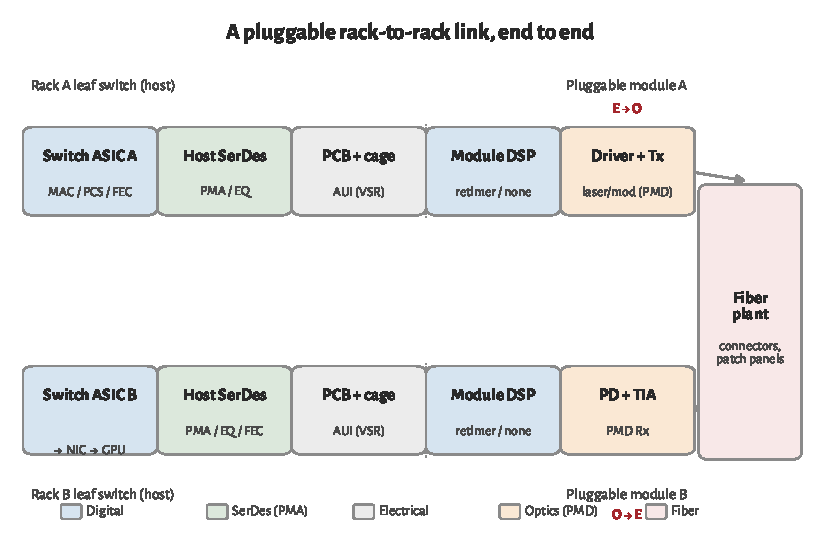
\includegraphics[width=\linewidth]{figures/fig_link_chain.pdf}
\caption{A pluggable rack-to-rack link, drawn as a folded loop. Transmit runs left to
right (switch ASIC $\to$ host SerDes $\to$ cage/AUI $\to$ module DSP $\to$ driver and
optics), the fiber turns the corner, and receive runs back into the far switch, then on
to the NIC and GPU. Colors mark the domain of each block; the two E$\leftrightarrow$O
crossings sit at the optics.\label{fig:link-chain}}
\end{figure}

This is the \emph{scale-out} path, the rack-to-rack Ethernet fabric where optics
already dominate. The \emph{scale-up} fabric that ties GPUs together
(NVLink- or UALink-class; \Cref{sec:scale-up-out}) is a different link. Its reach is
much shorter, so most of it is still copper: direct-attach cable or backplane under
roughly a meter, with no optics in the path at all. Optics only appears once rack
densification pushes those links past the copper wall, and even then it borrows the
same IM/DD building blocks over a different link and protocol layer. So the chain in
\Cref{fig:link-chain} is the one that carries the optical volume today; scale-up is
where optics is arriving next.

\section{Reach regimes, and the scope of this book}
\label{sec:reach}

``Optical interconnect'' is a wide phrase. A die-to-die link of a few millimeters
and a 10~km campus span both move bits on light, but they solve different
problems with different physics. AI compute fabrics live at the short end of that
spectrum, where lasers, IM/DD, and validation dominate cost, power, and
reliability. This book stays there and largely sets aside the 2--10~km campus and
data-center-interconnect links that have moved toward coherent optics.

\begin{table*}[ht]
\refstepcounter{table}\label{tab:reach}%
\centering
\setlength{\tabcolsep}{6pt}%
\begin{tabular}{@{}p{0.22\linewidth}p{0.18\linewidth}p{0.54\linewidth}@{}}
\toprule
Regime & Distance & Notes \\
\midrule
In-package / die-to-die & mm--cm & optical I/O chiplets (e.g. \Cref{sec:cwwdm}) \\
Chip-to-chip / co-packaged & cm & CPO engines on the switch/XPU substrate \\
Scale-up (rack scale) & $\sim$1--10~m & XPU-to-XPU; copper below $\sim$1--2~m, optics beyond \\
Intra-rack / intra-row & up to $\sim$100--500~m & SR over MMF; DR single-mode \\
\midrule
Campus / DCI \emph{(out of scope)} & 2~km (FR), 10~km (LR), and beyond & increasingly coherent, not IM/DD \\
\bottomrule
\end{tabular}
\par\medskip
{\raggedright\footnotesize\textbf{Table~\thetable.} Reach regimes. This book focuses on the top four.\par}
\end{table*}

The dividing line is roughly where a link leaves the compute fabric. Inside that
boundary, from millimeters in-package out to a few hundred meters, IM/DD is the
workhorse and the laser is the component that gates scale. That is the territory
this book treats.

\section{Where coherent takes over}
\label{sec:coherent-boundary}

\subsection{The two detection schemes, in one paragraph}

\term{IM/DD} encodes bits as changes in optical intensity and recovers them with a
square-law photodiode. Phase and polarization are discarded at detection. Coherent
detection mixes the received field against a narrow-linewidth local-oscillator (LO)
laser on a balanced photodiode pair, recovering amplitude and phase on both
polarizations. The receiver digitizes in-phase and quadrature samples and runs heavy
DSP: carrier recovery, polarization demux, chromatic dispersion compensation, and
soft-decision FEC. The coherent transmitter typically needs an I/Q modulator (or
equivalent) under the same linewidth discipline. That stack buys spectral
efficiency and reach tolerance. It costs extra photonic parts, ADC/DSP die area,
power, and latency.

\subsection{Why short reach stays IM/DD}

Inside the compute fabric, from millimeters in-package out to a few hundred meters
of single-mode fiber, loss and dispersion are modest: standard G.652.D fiber runs
about 0.2~dB/km at 1550~nm with a zero-dispersion wavelength near 1310~nm, so a
few hundred meters costs well under a decibel~\cite{itufiber}. A PAM4 IM/DD link
with equalization, FEC, and a reasonable laser closes without coherent mixing. The
energy argument from \Cref{ch:firstprinciples} applies directly: IM/DD keeps the
expensive digital work at the electrical ends where process scaling helps, and the
optical path is passive fiber. Rack and row runs also lean on bend-insensitive
G.657 fiber in patch panels and shelves, and the SR/DR reach classes below map onto
the OM4/OM5 multimode and OS1/OS2 single-mode cabling classes that ISO/IEC 11801
and TIA-492 define for the datacenter plant~\cite{fibercabling}. Retimed 800G
pluggables run roughly 14--18~W; LPO trims to roughly 7--9~W by deleting module
DSP~\cite{lpo}. A 400ZR-class coherent pluggable is built around a coherent DSP
that alone draws roughly 5--8~W inside a 15~W module budget~\cite{oif400zr},
landing near 45~pJ/bit at 400~Gb/s. Over a 100~m rack link that extra DSP power
does not buy enough margin to justify the BOM and service complexity
(\Cref{sec:power}).

\subsection{What coherent buys, and its price}

Coherent wins where the channel is harder: kilometers of fiber, amplified DWDM, and
dispersion that would crush a directly modulated PAM4 eye. Polarization multiplexing
and higher-order QAM raise bits per symbol. Electronic dispersion compensation
removes the need for tight wavelength and chirp control on the transmit laser. LO
mixing gives a sensitivity boost that IM/DD only matches with more launched power.
The price is upfront: linewidth requirements on both the transmit laser and the LO
(often well below 100~kHz for long reach), I/Q modulators or integrated coherent
PICs, high-speed ADCs, and a DSP that dominates module power. OIF standardized
400ZR coherent pluggables with a 15~W module budget for DCI spans to roughly
120~km~\cite{oif400zr}. ZR+ variants push reach further at similar or higher
power. That trade is right for campus and metro DCI. It is not the default inside
an AI rack.

\subsection{The crossover, and where it is moving}

Today the practical line sits near 2~km: intra-datacenter DR and shorter hops stay
IM/DD (\Cref{sec:reach,tab:ieee-lane}); campus FR/LR and DCI have moved to coherent
400ZR/ZR+ (\Cref{tab:reach}). Pressure pushes coherent inward on per-lane rates: at
224G and especially 448G the IM/DD SNR and TDECQ margin tighten, and some proposals
explore coherent-lite or coherent receivers for the longest scale-out
hops~\cite{cei448,e4ai448}. Pressure keeps IM/DD dominant for AI compute: LPO and
CPO attack the power wall (\Cref{sec:power,sec:224g-deploy}) by stripping module
DSP and shortening electrical reach, not by adding an LO and ADC chain. For
inference fabrics at in-package to a few hundred meters, IM/DD remains the workhorse
through the 224G generation. The open question is 448G and beyond: whether the
last scale-out meters stay PAM4/PAM6 IM/DD or whether a stripped coherent option
appears for links that already run retimed modules today (\Cref{sec:448g}).

\section{PAM4: more bits per symbol}

Through the 10G and early 25G eras, most short-reach optics used two-level NRZ:
one eye, one decision threshold, simple receivers. As per-lane rates climbed past
about 50~Gb/s, keeping NRZ would have demanded more electrical bandwidth than
connectors and SerDes could afford. The industry answer was \term{PAM4}: four
amplitude levels carrying two bits per symbol. Line rates below are in gigabaud
(\term{GBd}\firstterm{GBd}); host I/O is built in \term{SerDes}\firstterm{SerDes}
blocks.

\begin{table}[ht]
\centering
\caption{Per-lane rates and symbol rates (PAM4).\label{tab:pam4-rates}}
\begin{tabular}{@{}lll@{}}
\toprule
Per-lane rate & Symbol rate & Context \\
\midrule
100G/lane & $\approx$53.1~GBd & 400G/800G today \\
200G/lane & $\approx$106--112~GBd & 800G/1.6T ramp \\
224G/lane & $\approx$112~GBd (CEI-224G) & next SerDes generation \\
\bottomrule
\end{tabular}
\end{table}

PAM4 halves the required bandwidth versus NRZ for a given bit rate, but it costs
about 9.5~dB of SNR (three eyes instead of one, spaced one-third as far apart).
That SNR hit is why modern links assume equalization, DSP, and forward error
correction as part of the architecture rather than as optional polish
(\Cref{sec:equalization}). Looking ahead, the 448G debate is partly about whether
to stay on PAM4 at still higher baud or move to PAM6/PAM8 to ease the electrical
channel (\Cref{sec:448g}).

\section{Equalization and clock recovery}
\label{sec:equalization}

Once PAM4 became the default, the electrical channel stopped looking like a wire
and started looking like a filter. PCB traces, connectors, and cables low-pass
the signal; the receiver must undo that inter-symbol interference (ISI)\firstterm{ISI} before
slicing. Three equalizer classes appear in every short-reach link, plus clock
recovery when the bit clock is rebuilt.

\begin{description}
\item[CTLE (continuous-time linear equalizer)] \firstterm{CTLE} provides analog
      high-frequency boost, often a zero-pole pair in the SerDes front-end, the TIA,
      or a redriver chip. CTLE is cheap and low latency but fixed: it cannot adapt
      tap-by-tap to an arbitrary channel.
\item[FFE (feed-forward equalizer)] \firstterm{FFE} is a finite-impulse-response
      filter with pre- and post-cursor taps. Host SerDes and module DSPs use FFE
      (often with CTLE ahead of it) to open the eye.
      Transmitter and dispersion eye closure quaternary (TDECQ)\firstterm{TDECQ} applies a
      \emph{bounded} reference FFE when scoring transmitters (\Cref{sec:tdecq}).
\item[DFE (decision-feedback equalizer)] \firstterm{DFE} cancels post-cursor ISI
      using past symbol decisions. CEI electrical eye budgets reference an 8-tap DFE
      at the slicer (\Cref{sec:eye-budget}). DFE adds latency and error propagation
      but recovers more ISI than FFE alone at high loss.
\item[CDR (clock-data recovery)] \firstterm{CDR} extracts bit timing from the
      data stream and re-samples the eye. A \emph{retimer} includes CDR plus
      equalization and regenerates a clean output; a \emph{redriver} has CTLE/VGA but
      no CDR (\Cref{sec:conditioning}).
\end{description}

Where these blocks sit depends on the module style (\Cref{sec:pluggables,ch:networking}):

\begin{itemize}
\item \textbf{Fully retimed pluggable:} host SerDes $\to$ connector $\to$ module DSP
      (FFE/DFE/CDR) $\to$ optical engine. The module cleans a bad electrical channel.
\item \textbf{Redriver / ACC:} CTLE (+ VGA) in the cable or mid-channel; host SerDes
      still owns CDR and heavy EQ.
\item \textbf{LPO:} no module DSP/CDR. Host SerDes EQ and FEC must survive the full
      path; module may add only CTLE in the TIA and a linear driver
      (\Cref{sec:conditioning}). Optical TDECQ and electrical margin both tighten.
\end{itemize}

\Cref{fig:eq-chains} shows the correct SerDes equalizer order, then where those
blocks live in a retimed module versus LPO.

\begin{figure}[ht]
\centering
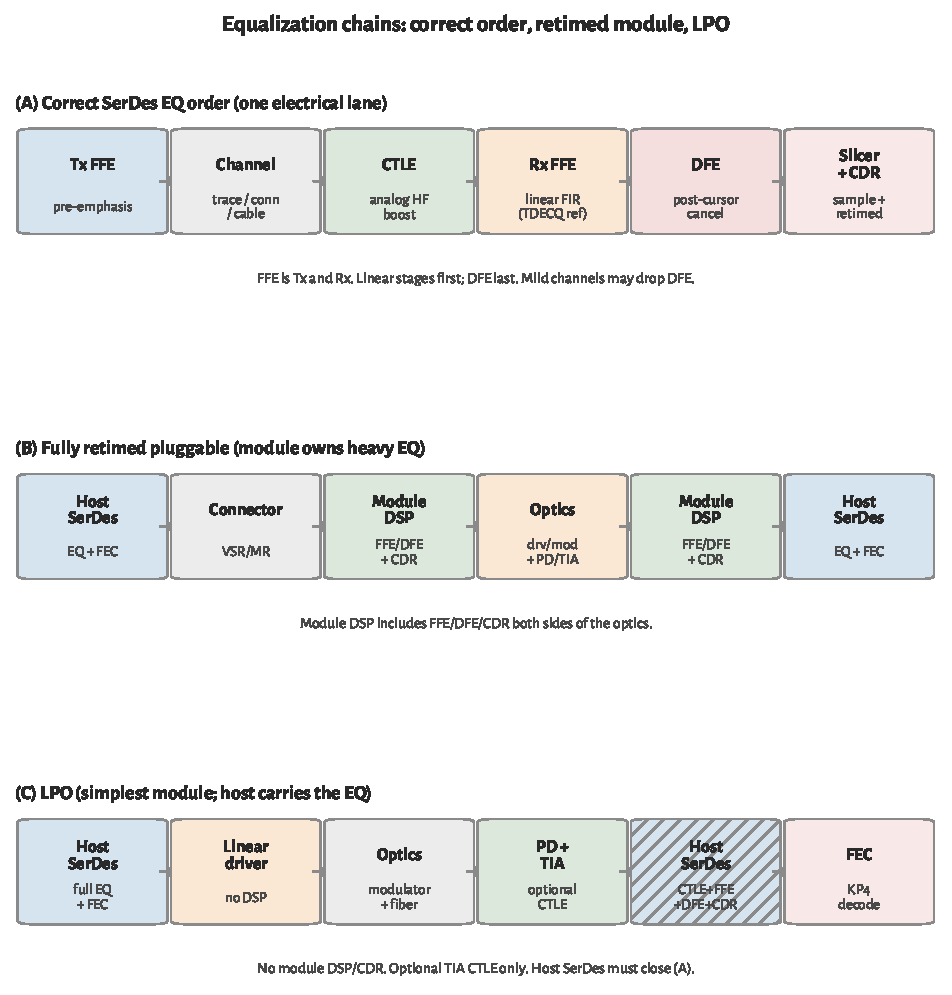
\includegraphics[width=\linewidth]{figures/fig_eq_chains.pdf}
\caption{Equalization chains. (A)~Correct order on one electrical lane: Tx FFE,
channel, CTLE, Rx FFE, DFE, then slicer/CDR. (B)~Fully retimed pluggable: module
DSP owns FFE/DFE/CDR on both sides of the optics. (C)~LPO: no module DSP; the host
SerDes must close the full EQ and FEC path.\label{fig:eq-chains}}
\end{figure}

\keyidea{CTLE boosts analog bandwidth; FFE/DFE cancel ISI digitally; CDR rebuilds
timing in retimers. LPO deletes the module-side safety net, so host equalization and
KP4 margin (\Cref{sec:kp4}) become the whole electrical story.}

\section{SerDes and DSP: who does the work}
\label{sec:serdes-dsp}

The equalizers above have to run somewhere, and ``SerDes'' and ``DSP'' get used
loosely for that somewhere. They are not the same thing, and at 112~GBd the line
between them has mostly dissolved. Pinning down the vocabulary makes the retimed
versus LPO versus CPO argument (\Cref{sec:conditioning,ch:networking}) concrete
instead of a wall of acronyms.

\subsection{What the SerDes is}

\term{SerDes} is the high-speed electrical I/O macro on an ASIC: switch silicon, a
NIC, an accelerator, or a module chip. On transmit it serializes wide, slow
parallel data from the MAC/PCS into one PAM4 lane on the wire; on receive it
deserializes the sampled lane back to parallel words. That is the literal
serializer/deserializer job. Everything else the SerDes does is in service of
getting a clean symbol stream across a lossy channel.

\subsection{Analog SerDes versus DSP-based SerDes}

How the SerDes conditions the signal splits into two design styles. An
\emph{analog} (mixed-signal) SerDes equalizes in the analog domain (CTLE, a few
analog FFE/DFE taps) and slices directly. It is low power and low latency but
limited in how much loss it can undo and how flexibly it adapts. A
\term{DSP-based}\firstterm{dspserdes} SerDes puts a high-speed ADC on the receive
lane, digitizes the eye, and does FFE, DFE, and timing recovery numerically, with
a DAC and digital pre-distortion on transmit. It burns more power and adds
latency, but it closes far more channel loss and adapts tap-by-tap. Above roughly
50~GBd the DSP-based architecture won: 112~GBd (224G) host SerDes and module
retimers are ADC/DSP designs. So the ``DSP'' that cancels ISI at 224G usually lives
\emph{inside} the SerDes, not in a separate chip.

\subsection{Two things people call ``the DSP''}

That is the first meaning of DSP: the digital equalization and clock recovery
inside a modern SerDes. The second meaning is \emph{the module DSP}, a distinct
retimer chip in a pluggable that has its own ADC/DSP SerDes on the host side, an
FFE/DFE/CDR core, a gearbox (\Cref{sec:gearbox}), and often the FEC engine, then
drives the optics. When the book says a retimed module ``has a DSP'' and LPO
``deletes the DSP'' (\Cref{sec:conditioning}), it means this second chip. Deleting
it does not delete DSP from the link; it moves the equalization burden back onto
the \emph{host} SerDes DSP and onto FEC.

\subsection{Where FEC sits}

FEC is a third block, and it is usually not part of the SerDes proper. KP4 encode
and decode live in the PCS/FEC layer on the host (or in the module DSP when one is
present), operating on the recovered symbol stream (\Cref{sec:kp4}). This is why a
link can have a healthy SerDes eye and still fail on FEC, or ride an ugly eye that
KP4 cleans: the SerDes recovers symbols, FEC fixes what is left. Validation reads
pre-FEC BER exactly at that SerDes-to-FEC boundary.

\subsection{Mapping it back to module styles}

\Cref{tab:serdes-dsp} sorts the blocks by where they physically run for the three
module styles. \Cref{fig:eq-chains} shows the same split as signal chains. Read the
LPO column as the design point that matters most for AI power budgets: the host
SerDes DSP and host FEC carry the entire electrical channel, because the module has
no retimer to hide behind (\Cref{sec:224g-deploy}).

\begin{table}[ht]
\centering
\caption{Where each block runs, by module style.\label{tab:serdes-dsp}}
\setlength{\tabcolsep}{4pt}%
\footnotesize
\begin{tabular}{@{}p{0.24\linewidth}p{0.22\linewidth}p{0.20\linewidth}p{0.22\linewidth}@{}}
\toprule
Block & Retimed & LPO & CPO (XSR) \\
\midrule
Serialize / PAM4 & Host SerDes & Host SerDes & Host SerDes \\
Rx EQ (FFE/DFE) & Module DSP & Host SerDes DSP & Host SerDes DSP \\
CDR / retiming & Module DSP & Host SerDes & Host SerDes \\
KP4 FEC & Host (or module) & Host & Host \\
Optical drive & Module DSP out & Linear driver & On-package engine \\
\bottomrule
\end{tabular}
\end{table}

\keyidea{The SerDes is the ASIC's electrical PHY; at 224G its equalization and clock
recovery are done in DSP inside the SerDes. ``The module DSP'' is a separate
retimer chip. LPO removes that retimer, so the host SerDes DSP plus KP4 FEC
(\Cref{sec:kp4}) own the whole electrical channel. Optics begin only after that
handoff.}

\section{The Ethernet PHY stack: where optics attaches}
\label{sec:phy-stack}

The SerDes, the FEC, and the optics are not loose parts. IEEE 802.3 stacks them into
named sublayers, and knowing the stack tells you exactly where the optical
transceiver plugs in and which block owns each impairment. Ethernet lives at the
bottom two OSI layers: the \term{MAC}\firstterm{MAC} (data link) builds frames and carries the
addressing, and the \term{PHY}\firstterm{PHY} (physical) turns those frames into
signals on the wire. Everything in this book sits inside the PHY.

\subsection{The sublayers, top to bottom}

The PHY is itself a stack. \Cref{tab:phy-stack} lists the sublayers a 400G/800G port
walks through on transmit (receive runs in reverse).

\begin{table}[ht]
\centering
\caption{IEEE 802.3 PHY sublayers, transmit order.\label{tab:phy-stack}}
\setlength{\tabcolsep}{4pt}%
\footnotesize
\begin{tabular}{@{}p{0.14\linewidth}p{0.52\linewidth}p{0.24\linewidth}@{}}
\toprule
Sublayer & Function & Domain \\
\midrule
MAC & Frame, address, CRC & Digital, host \\
RS & Reconciliation: adapt MAC to the PHY across the xMII & Digital, host \\
PCS & 64B/66B, 256B/257B transcode, scramble, RS-FEC & Digital \\
PMA & Serialize, lane mux, clock recovery (SerDes) & Mixed-signal \\
PMD & Modulate/detect light: laser, driver, PD, TIA & Optical \\
\bottomrule
\end{tabular}
\end{table}

Two interface names sit between these blocks and cause most of the confusion. The
\term{xMII}\firstterm{xMII} (for example 400GMII) is a wide parallel bus inside the
chip between MAC and PCS. The \term{AUI}\firstterm{AUI} (for example 400GAUI-4) is the
electrical serial lane set that leaves the host and crosses the faceplate connector
to the module. The AUI is the CEI electrical channel your SerDes has to survive
(\Cref{sec:serdes-dsp,ch:networking}); the \term{PMD}\firstterm{PMD} is the optical
transceiver on the far side of it.

\subsection{Where the optics attaches}

Optics is the PMD, and only the PMD. Everything above it is electrical or logical and
is medium-independent: the same MAC, RS, PCS, and PMA feed a copper DAC, a
multimode SR module, or a single-mode DR module. That is the whole point of the
layering. When IEEE names \texttt{400GBASE-DR4} or \texttt{800GBASE-DR8}, it is
naming a PMD (\Cref{sec:pmd-reach}); the digital stack above is shared. It is also
why the retimed-versus-LPO-versus-CPO argument is really about \emph{where the PMA
and PCS/FEC physically sit} relative to the AUI, not about changing the optics
(\Cref{sec:serdes-dsp}).

\subsection{Line-rate accounting}

The layering is where the MAC-rate-versus-line-rate gap (\Cref{tab:rate-stack})
actually comes from. Take one 400G port. The MAC delivers 400~Gb/s of payload. The
PCS transcodes it (256B/257B adds about 0.4\%) and then RS(544,514) FEC adds 30
parity symbols per 514 data symbols, a $544/514$ expansion of roughly 5.8\% relative
to payload (equivalently 5.5\% of the coded line, \Cref{sec:kp4}). The two multiply
out to $257/256 \times 544/514 = 1.0625$, so the line carries $400 \times 1.0625 =
425$~Gb/s, split as four AUI lanes at 106.25~Gb/s (53.125~GBd PAM4). The optical PMD
carries that same 425~Gb/s. So ``400G Ethernet'' is a 400~Gb/s MAC rate riding a
425~Gb/s line, and the extra 25~Gb/s is transcode plus FEC, not wasted bandwidth.

\subsection{What the PCS actually does}

Inside the PCS\firstterm{PCS}, the MAC's 64-bit words are first wrapped in 64B/66B blocks: a 2-bit
sync header (\texttt{01} for data, \texttt{10} for control) lets the receiver find
block boundaries in the serial stream. Four 66-bit blocks are then transcoded into
one 257-bit block, which compresses the four 2-bit sync headers to a single bit and,
crucially, produces a 256-bit payload that aligns cleanly with 10-bit RS-FEC symbols
($\mathrm{lcm}(256,10)=1280$, so five blocks make exactly 128 symbols with no
remainder). The RS(544,514) encoder then adds parity (\Cref{sec:kp4}), and the PMA
distributes the coded symbols across logical lanes, bit-multiplexes them down to the
physical AUI lanes, and serializes each to PAM4. The payload bits themselves are
never altered by transcoding; only the framing overhead is squeezed.

Where these blocks physically live is an implementation choice, not a layer rule.
The PCS/FEC can sit in the host switch ASIC or in a module retimer DSP; LPO deletes
the module DSP and forces the host to own PCS/FEC and all of the PMA equalization
(\Cref{sec:serdes-dsp,sec:conditioning}). The layer names stay the same regardless of
which chip runs them.

\keyidea{Ethernet is MAC (frames) plus PHY, and the PHY is RS, PCS, PMA, PMD.
Optics is only the PMD; everything above is medium-independent, which is why one
digital stack feeds copper, multimode, or single-mode. The MAC-to-line-rate gap is
transcode ($257/256$) times FEC ($544/514$), giving 425~Gb/s on a 400G port. The
module-style debate is about which side of the AUI runs the PMA and PCS/FEC.}

\section{Test points: where the link is measured}
\label{sec:test-points}

Every metric in this book is taken \emph{somewhere}. A datasheet line like
``TDECQ~$\le$~3.4~dB'' or ``stressed sensitivity $-3.1$~dBm'' means nothing until you
name the reference plane it was measured at. The standards name those planes TP0
through TP5, plus the host-referenced pair TP1a and TP4a, and they run in order from
the transmit silicon to the receive silicon. Learning them turns a scattered pile of
numbers into a map: each spec belongs to exactly one plane, and each plane is owned
by one document. \Cref{fig:test-points} walks the chain; \Cref{tab:test-points}
is the lookup card.

The mistake to avoid is treating TP2 and TP3 as electrical points just past a
connector. They are \emph{optical} planes at the fiber. TP2 is the light launched
into the fiber, measured after the module's electrical-to-optical conversion (driver
plus laser or modulator). TP3 is the light arriving at the far module, before its
optical-to-electrical conversion (photodiode plus TIA). The electrical planes are the
ones on either side of those two crossings.

\begin{figure}[ht]
\centering
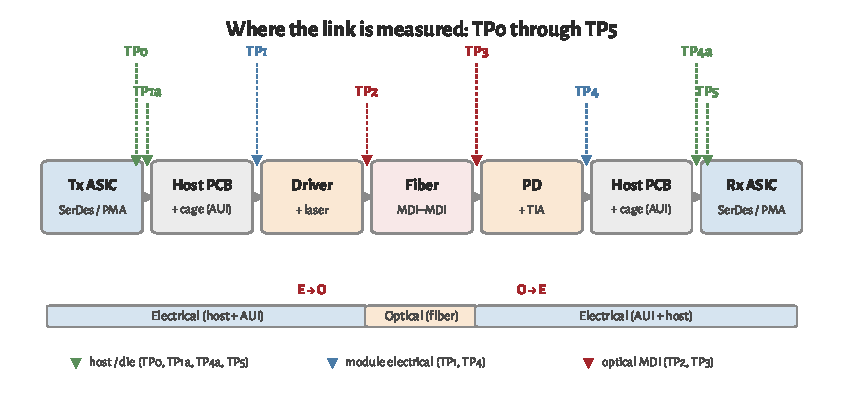
\includegraphics[width=\linewidth]{figures/fig_test_points.pdf}
\caption{Test points on a one-way IM/DD link. Green marks the host and die-pad
electrical planes (TP0, TP1a, TP4a, TP5); blue the module's electrical connector
(TP1, TP4); red the optical planes at the fiber \term{MDI} (TP2, TP3).
The two domain crossings, E$\to$O in the module transmitter and O$\to$E in the module
receiver, sit between the electrical and optical planes.\label{fig:test-points}}
\end{figure}

\newthought{Read the chain in order.} At the transmit end, \textbf{TP0} is the
transmit SerDes output at the die pad, the silicon designer's reference. \textbf{TP1a}
is the same host signal referenced at the module cage, the \term{AUI} the module must
accept; its electrical eye quality is \term{EECQ}\firstterm{EECQ}, the electrical
analog of TDECQ. \textbf{TP1} is the module's electrical input on the far side of the
mated connector. The module then converts electrical to optical, and \textbf{TP2} is
the optical launch at the transmitter \term{MDI}\firstterm{MDI}, where TDECQ, TECQ, OMA$_{\mathrm{outer}}$,
ER, and RIN are specified (\Cref{ch:validation,sec:tdecq}). After the fiber,
\textbf{TP3} is the optical input at the receiver MDI, where stressed receiver
sensitivity (SECQ) is specified. The module converts back to electrical at
\textbf{TP4} (its electrical output), \textbf{TP4a} is the host-referenced input near
the receive SerDes under worst-case module output, and \textbf{TP5} is the receive
die pad.

\begin{table*}[ht]
\refstepcounter{table}\label{tab:test-points}%
\centering
\setlength{\tabcolsep}{5pt}%
\footnotesize
\begin{tabular}{@{}p{0.05\linewidth}p{0.075\linewidth}p{0.29\linewidth}p{0.30\linewidth}p{0.15\linewidth}@{}}
\toprule
Point & Domain & Location & Principal measurement & Owning spec \\
\midrule
TP0 & Electrical & Tx ASIC/SerDes die pad (host) & Silicon Tx quality; design reference, hard to probe once packaged & OIF CEI C2M \\
TP1a & Electrical & Host output at the cage, host-referenced (SerDes output via a host compliance board) & Host Tx eye, EECQ; the AUI the module must accept & OIF CEI C2M; LPO MSA \\
TP1 & Electrical & Module electrical input (module side of the mated connector) & Module input stressor calibration & IEEE 802.3 AUI; OIF CEI \\
TP2 & Optical & Transmitter MDI, fiber launch (after E$\to$O) & TDECQ, TECQ, OMA$_{\mathrm{outer}}$, ER, RIN$_x$OMA & IEEE 802.3 PMD; LPO MSA \\
TP3 & Optical & Receiver MDI, fiber input (before O$\to$E) & Stressed receiver sensitivity, SECQ & IEEE 802.3 PMD; LPO MSA \\
TP4 & Electrical & Module electrical output (module side of the connector) & Module Rx electrical output, EECQ & IEEE 802.3 AUI; OIF CEI \\
TP4a & Electrical & Stressed host input, host-referenced (near the Rx SerDes) & Host Rx under worst-case module output & OIF CEI C2M; LPO MSA \\
TP5 & Electrical & Rx ASIC/SerDes die pad (host) & Silicon Rx recovery; design reference, hard to probe & OIF CEI C2M \\
\bottomrule
\end{tabular}
\par\medskip
{\raggedright\footnotesize\textbf{Table~\thetable.} Test-point reference planes on a
short-reach IM/DD link, transmit to receive. The optical planes TP2 and TP3 carry the
transmitter- and receiver-quality specs; the electrical planes carry the host and
module eye specs. See \Cref{tab:lpo-tp} for the concrete LPO MSA assignments.\par}
\end{table*}

\newthought{Who owns which plane.} The split is not arbitrary. IEEE 802.3 optical PMD
clauses define the transceiver planes: the optical TP2 and TP3, and the module's
electrical PMD input and output at TP1 and TP4~\cite{ieee8023dj}. The OIF Common
Electrical I/O chip-to-module work owns the electrical planes deeper into the host:
the die pads TP0 and TP5, and the host-referenced compliance points TP1a and TP4a,
which are measured through host and module compliance boards to de-embed the
fixture~\cite{cei224}. The LPO MSA then binds both sides into a single product
contract for a DSP-less module, with the six-point ladder (TP1a, TP1, TP2, TP3, TP4,
TP4a) tabulated in \Cref{tab:lpo-tp}~\cite{lpomsa}.

The numbering is a family of conventions, not one universal set. IEEE optical PMD
clauses commonly define only TP1 through TP4, with the optical measurements at TP2
and TP3; the die pads TP0/TP5 and the host-referenced TP1a/TP4a come from the
chip-to-module electrical world. Fibre Channel historically used its own reference
points. Match the labels to the document you are reading rather than assuming a shared
TP0-to-TP5 spine.

\newthought{Where compliance testing concentrates.} Optical transmitter compliance
lives at TP2 (TDECQ, OMA, ER); optical receiver compliance lives at TP3 (stressed
sensitivity). Electrical host and module compliance concentrate at TP1a and TP4a,
which is why a module that passes optical TDECQ at TP2 can still fail interop if it
misses EECQ at TP1a. TP0 and TP5 sit inside the package and are informative for
silicon design but hard to probe in a finished system. A retimed module recovers the
signal before TP4; a linear (LPO) module does not, so at 224G its host EQ and FEC
carry the whole electrical channel (\Cref{sec:conditioning,sec:pmd-reach}).

\keyidea{The plane makes the number. TP2 and TP3 are optical, at the fiber MDI, and
carry transmitter and receiver quality (TDECQ, stressed sensitivity). TP1 and TP4 are
the module's electrical connector; TP1a and TP4a are host-referenced near the SerDes;
TP0 and TP5 are the die pads. IEEE 802.3 owns the optical planes, OIF CEI owns the
die and host-referenced electrical planes, and the LPO MSA binds all of them into one
DSP-less product contract (\Cref{tab:lpo-tp}).}

\section{The link-budget vocabulary}

These terms are the language of both datasheets and debug. Learn them as a
ledger, not as a glossary quiz: when a link fails, you are almost always arguing
about one of them.

\begin{description}
\item[OMA (optical modulation amplitude)] \firstterm{OMA} $P_1 - P_0$: the real signal swing.
      For PAM4 the ``outer OMA'' spans the outermost levels.
\item[Extinction ratio (ER)] \firstterm{ER} $P_1/P_0$, in dB. Trades against insertion loss and
      against \term{TDECQ} (\Cref{ch:validation}).
\item[RIN (relative intensity noise)] \firstterm{RIN} the laser's own amplitude noise; sets a
      noise floor that matters more as OMA shrinks.
\item[Chirp] the unwanted frequency modulation that accompanies intensity
      modulation. Large in directly modulated lasers; small and controllable in
      externally modulated lasers. See \Cref{sec:chirp-dispersion}.
\item[Chromatic dispersion penalty] dispersion $\times$ chirp $\times$ distance
      produces inter-symbol interference. This drives the wavelength plan and the
      choice between directly and externally modulated lasers (\Cref{sec:chirp-dispersion}).
\item[Receiver sensitivity] the minimum OMA needed to hit a target bit-error
      ratio; ``stressed'' sensitivity adds a calibrated impairment for margin.
\end{description}

\aside{A clean mental model: start with transmitter OMA, subtract connector and
fiber loss, subtract penalties (dispersion, TDECQ, reflection), and compare the
result to receiver sensitivity (\Cref{sec:sensitivity,ch:models,sec:link-budget}). What remains is margin.}

\section{Chirp, dispersion, and the IM/DD penalty}
\label{sec:chirp-dispersion}

IM/DD detects power, not phase, but phase still matters on the fiber. Intensity
modulation couples to frequency through the laser or modulator \emph{chirp}
parameter $\alpha$: a change in output power shifts the instantaneous optical
frequency. Single-mode fiber then converts that frequency wander into intensity
distortion via chromatic dispersion (different $\lambda$ travel at slightly
different speeds).

The penalty grows with chirp $\times$ dispersion $\times$ distance. At O-band
($\sim$1310~nm) dispersion is near zero ($|D|\lesssim 3$~ps/(nm$\cdot$km)), which is why
silicon photonics and many datacenter SMF\firstterm{SMF} links use 1310~nm class wavelengths. At
C-band ($\sim$1550~nm) dispersion is larger; chirpy sources pay more per kilometer.

Source choice sets chirp (\Cref{ch:lasers,tab:tx-modulator,sec:eml-eam}):

\begin{itemize}
\item \textbf{DML:} large $\alpha$; fine for tens of meters of MMF or uncooled SR,
      poor for FR-class SMF unless rate and reach stay short.
\item \textbf{EML / external MZM / ring:} low chirp; default for DR/FR and CPO.
\item \textbf{Reflections:} light reflected back into the laser raises effective
      chirp and RIN; optical return loss (ORL)\firstterm{ORL} specs exist for this reason
      (\Cref{sec:optical-channel}).
\end{itemize}

For the distances this book treats (in-package through a few hundred meters), dispersion
is often secondary to TDECQ, connector loss, and receiver noise. It becomes decisive
when a low-chirp assumption fails (aging EAM bias, DML on SMF, or FR edge cases).
TDECQ embeds dispersion in its name because the reference receiver includes a
dispersion penalty model for the standardized test channel.

\section{Forward error correction}
\label{sec:kp4}

Modern PAM4 links do not meet raw bit-error-ratio targets on their own; they lean
on \term{FEC}\firstterm{FEC}. The datacenter workhorse is \term{KP4}\firstterm{KP4}, a Reed--Solomon code
RS(544,514)\firstterm{RS544514} operating on 10-bit symbols. The name comes from
\texttt{100GBASE-KP4} in IEEE 802.3bj: K for backplane, P for PAM4, 4 for four
lanes~\cite{ieee8023bj}. Today ``KP4'' means that FEC code on any
PAM4 Ethernet link (optical DR, 224G SerDes, and backplane), not only the original
backplane PHY. The link is specified to a
\emph{pre-FEC}\firstterm{preFEC} BER threshold, on the order of $2.4\times10^{-4}$, which FEC then
drives down to an effectively error-free \emph{post-FEC}\firstterm{postFEC} BER.

Two consequences matter in practice:

\begin{enumerate}
\item Validation targets are stated in pre-FEC BER, and FEC symbol-error
      histograms are a rich debug signal (they reveal \emph{how} a link is
      failing, not just that it is).
\item Emerging \term{linear-drive} optics (\term{LPO}\firstterm{LPO}/\term{LRO}\firstterm{LRO}, \Cref{ch:networking}) remove
      the DSP/retimer to save power, which tightens the link budget and leans
      even harder on FEC and on transmitter quality (\Cref{sec:equalization}).
\end{enumerate}

\paragraph{KP4 in practice.}

\term{KP4} maps to Reed--Solomon RS(544,514) on 10-bit symbols: 514 payload symbols,
30 parity, up to 15 correctable symbol errors per codeword. Coding overhead is
$30/544\approx5.5\%$, so the \emph{line rate} on the wire exceeds the MAC/info rate
(for example, 802.3dj delivers $\approx$211~Gb/s payload on a 224~Gb/s PAM4 lane).
\Cref{tab:rate-stack} is the decoder for the three rate names you will see in
802.3dj and CEI-224G docs (example: one 200G Ethernet lane).

\begin{table}[ht]
\centering
\caption{Three rate names on one 802.3dj lane (200G Ethernet).\label{tab:rate-stack}}
\begin{tabular}{@{}p{0.18\linewidth}p{0.42\linewidth}p{0.32\linewidth}@{}}
\toprule
Term & Meaning & Example \\
\midrule
MAC rate & User Ethernet throughput at MAC & 200~Gb/s per lane \\
Line rate & Bits on wire incl.\ FEC overhead & $\sim$211--224~Gb/s (context-dependent) \\
Symbol rate & Baud on the electrical/optical lane & $\sim$112~GBd PAM4 \\
\bottomrule
\end{tabular}
\end{table}

The optical PHY is qualified to a \emph{pre-FEC} BER threshold, typically
$2.4\times10^{-4}$ for KP4-class links. That corresponds to $Q\approx3.5$ on the
Gaussian model of \Cref{sec:qber}. Post-FEC the target is effectively error-free
($10^{-12}$ to $10^{-15}$ class). Validation always reports pre-FEC BER during
bring-up; post-FEC confirms the decoder is working.

FEC symbol-error \emph{histograms} are a debug tool: clustered errors point to
burst impairments (reflections, power droop); sparse errors point to Gaussian noise
margin. At 448G/lane, CEI notes that KP4 at $10^{-4}$ pre-FEC may not close on
40~dB-class channels without stronger codes (\Cref{tab:448-fec}): MLC plus higher
overhead RS, or hard-decision FEC in demos (\Cref{sec:448g}).

\section{Ethernet optical PMDs and reach classes}
\label{sec:pmd-reach}

IEEE 802.3 names the optical transceiver (\term{PMD}) separately from
the MAC rate. Short-reach IM/DD classes that matter for AI fabrics:

\begin{description}
\item[SR (short reach)] \firstterm{SR} multimode fiber, VCSEL at 850~nm or evolving MMF\firstterm{MMF} solutions;
      rack and row distances; modal noise and bandwidth limit legacy SR.
\item[DR (datacenter reach)] \firstterm{DR} single-mode, typically 500~m class at 1310~nm; PAM4,
      KP4, TDECQ limits; the mainstream 400G/800G/1.6T module reach.
\item[FR (far reach)] \firstterm{FR} single-mode, 2~km class; same optics family as DR with tighter
      transmitter specs; chirp and dispersion matter more at the margin.
\end{description}

Naming examples: 400G-DR4 (four lanes), 800G-DR8, 800G-FR8 (eight $\lambda$, 2~km).
802.3dj adds 200G/lane Ethernet; the 400G/lane study group targets the next
generation (\Cref{tab:ieee-lane,sec:448g}). Campus LR and coherent DCI sit beyond
this book's scope (\Cref{tab:reach}).

\section{The per-lane roadmap: 224G and beyond}
\label{sec:224g}

Per-lane rate is the axis the whole industry advances along, because doubling it
roughly doubles switch and module capacity for the same lane count. The electrical
I/O roadmap is set by the OIF's Common Electrical I/O (CEI) projects, and optics
tracks it closely.

\begin{table}[ht]
\centering
\caption{The CEI per-lane roadmap.\label{tab:cei-roadmap}}
\begin{tabular}{@{}llll@{}}
\toprule
Generation & Per lane & Modulation & Ethernet rates \\
\midrule
CEI-112G & 112~Gb/s & PAM4 & 100/200/400G \\
CEI-224G & 224~Gb/s & PAM4 ($\approx$112~GBd) & 200/400/800/1600G \\
CEI-448G & 448~Gb/s & TBD (PAM4/6/8) & 400/800/1600/3200G \\
\bottomrule
\end{tabular}
\end{table}

\Cref{fig:cei-rate-year} puts that ladder on a longer clock: OIF CEI has roughly
doubled the rate per differential pair every four to five years since the early
2000s. Open markers for 224G and 448G follow the demo deck's ``202X'' placement;
224G is shipping now, 448G is still pathfinding~\firstcite{cei224}.

\begin{figure}[ht]
\centering
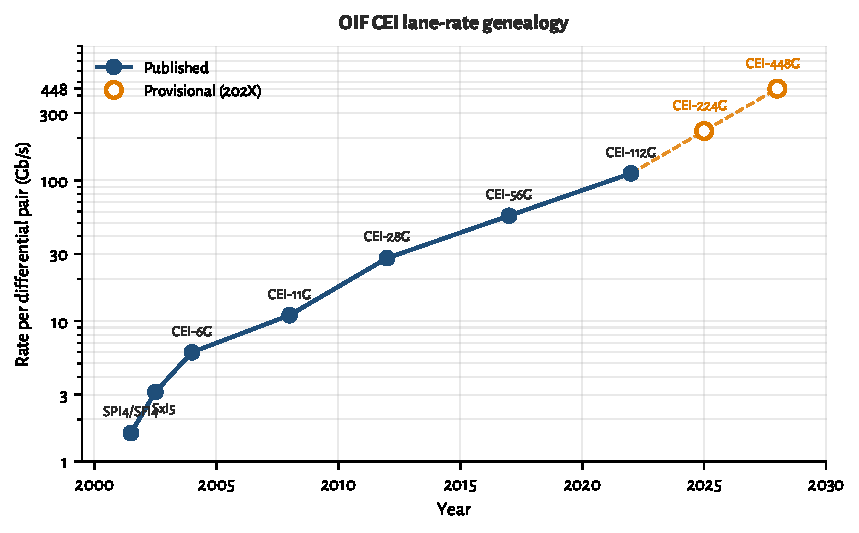
\includegraphics[width=0.92\linewidth]{figures/fig_cei_rate_vs_year.pdf}
\caption{OIF CEI rate per differential pair versus year (log scale). Data from the
OFC~2025 CEI interoperability demo genealogy; 224G/448G years are provisional
placements for the deck's 202X entries, and 448G's rate is the naming target
(PAM order still open).\label{fig:cei-rate-year}}
\end{figure}

\subsection{224G is settled; the frontier is deployment}

\term{CEI-224G} kicked off in 2022 as the electrical follow-on to CEI-112G. It
kept PAM4 and roughly doubled the baud, to about 112~GBd per lane, with reach
projects from XSR through LR now maturing. That choice is no longer the open
debate; it is the shipping baseline. Eight 224G lanes make a 1.6~Tb/s port, and
the same SerDes generation feeds 102.4~Tb/s-class switch silicon
(\Cref{sec:cpo-status}). Copper reach has collapsed to about a meter, DSP-based
SerDes are assumed, and a \term{CEI-224G-Linear} variant defines linear operation
without a DSP/retimer in the optical module: the electrical foundation for LPO
(\Cref{ch:networking}). The remaining work is deployment: closing LPO margins,
qualifying ELSFP banks for CPO, and holding yield at volume, not inventing a new
modulation alphabet.

\Cref{fig:cei-reach-map} is the reach map those projects sit on: \term{XSR}/XSR+
inside the package (die-to-die and die-to-optical-engine), \term{VSR} from ASIC to
a faceplate pluggable, \term{MR} chip-to-chip on the board (PCB or twinax), and
\term{LR} for backplane and longer copper cables~\firstcite{cei224}. The media
labels (host PCB traces, twinax, optical fiber, optical module) are where the
loss budget actually lives; the CEI class name is the electrical recipe for that
hop. \Cref{tab:cei224-reach} is the matching lookup card from the CEI-224G project
map (OFC~2025 demo framing)~\firstcite{cei224demo,cei224}.

\begin{figure}[ht]
\centering
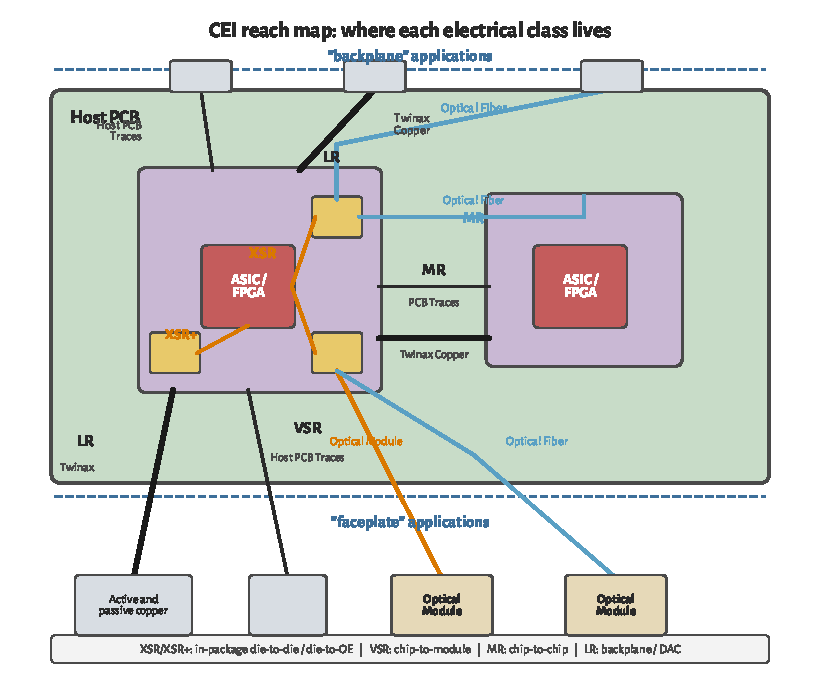
\includegraphics[width=\linewidth]{figures/fig_cei_reach_map.pdf}
\caption{CEI reach map on a host PCB (redrawn). Backplane applications sit above
the board; faceplate cages and modules sit below. XSR/XSR+ are in-package;
VSR is chip-to-module; MR is chip-to-chip; LR covers backplane and active/passive
copper.\label{fig:cei-reach-map}}
\end{figure}

\begin{table*}[ht]
\refstepcounter{table}\label{tab:cei224-reach}%
\centering
\setlength{\tabcolsep}{4pt}%
\footnotesize
\begin{tabular}{@{}p{0.12\linewidth}p{0.22\linewidth}p{0.28\linewidth}p{0.30\linewidth}@{}}
\toprule
Class & Hop & Nominal reach / channel & Notes \\
\midrule
XSR & Die-to-die or die-to-OE & $\lesssim$50~mm package substrate & CPO / chiplet optics; light EQ \\
VSR & Chip-to-pluggable module & $\sim$200~mm host + $\sim$20~mm module, 1 connector & Classic faceplate retimed path \\
MR & Chip-to-chip / midplane & $\sim$500~mm, 1 connector & Board-scale copper \\
LR & Backplane or copper cable & $\sim$1000~mm host+daughter, 2 connectors & DAC/ACC/AEC territory \\
Linear & Chip-to-linear module & Same cages as VSR-class ports; no module DSP & LPO foundation; host EQ + FEC \\
\bottomrule
\end{tabular}
\par\medskip
{\raggedright\footnotesize\textbf{Table~\thetable.} CEI-224G electrical classes (project map).
BER target on the reach classes is $10^{-15}$ or better with FEC allowed. Draft
LR/MR IAs were member-review as of OFC~2025; Linear is the separate full-linear
module track.\par}
\end{table*}

One SerDes core may not cover XSR through LR efficiently: short reaches want
simple, low-power equalization, while LR burns DSP to close tens of dB of loss.
That is why Linear is its own project rather than ``VSR with the DSP deleted,''
and why CPO (XSR) and LPO (Linear) show up as different power/serviceability bets
(\Cref{sec:224g-deploy,sec:pluggables,sec:cpo-status}).

\subsection{Deploying 224G: LPO, COM, and TDECQ corners}
\label{sec:224g-deploy}

At 224G the alphabet is settled (PAM4 + KP4). What fails in the field is the
\emph{margin stack}: electrical channel operating margin (COM) on the host side,
transmitter and dispersion eye closure quaternary (TDECQ) on the optical side,
and the production corners that couple them (\Cref{sec:prod-corners}). Retimed
modules still dominate 1.6T faceplate ports because their DSP absorbs host-channel
sin. LPO and LRO exist to delete that DSP for power and latency; they only ship
when both ledgers close without it~\firstcite{lpo,cei224,semtech224}.

\paragraph{The two ledgers that must close together.}
A retimed module can hide a bad host PCB behind module EQ. An LPO module cannot.
You therefore run two go/no-go tests as one program:

\begin{description}
\item[Electrical COM] After the CEI reference TX, channel, and Rx (CTLE + 8-tap
      DFE), COM\firstterm{COM} $\ge3$~dB is the usual pass line at the slicer
      (\Cref{sec:com,sec:eye-budget}). At 112~GBd the residual eye after that
      equalizer is only a few millivolts tall; KP4 then cleans pre-FEC BER near
      $2.4\times10^{-4}$ down to $10^{-15}$ class (\Cref{sec:kp4}).
\item[Optical TDECQ / TECQ] Outer OMA, RLM, and TDECQ (or \term{TECQ}\firstterm{TECQ} without the test
      fiber) score the transmitter after a bounded reference FFE
      (\Cref{sec:tdecq}). LPO MSA language for 100G/lane DR already couples OMA
      to max(TECQ, TDECQ) and caps TDECQ near 3.4~dB; 224G-class linear modules
      inherit the same philosophy even while CEI-224G-Linear and IEEE 802.3dj
      freeze the exact limits~\firstcite{lpomsa,ieee8023dj,cei224}.
\end{description}

CEI-224G-Linear defines the host/module electrical test points (TP1/TP1a,
TP4/TP4a) so a linear module can sit between a DSP host SerDes and the fiber
without its own CDR~\firstcite{cei224}. Commercial 224G driver/TIA families
advertise that interface explicitly (tunable swing, on-chip CTLE, CEI-224G-Linear
host EQ)~\citehref{semtech224}{Semtech 224G}. If either ledger is soft, prefer
retimed or LRO until the host PCB and module linearity improve; do not ``fix''
LPO with more FEC alone.

\paragraph{Where 224G LPO programs actually break.}
The failure modes are familiar once you stop treating LPO as a cheaper OSFP:

\begin{itemize}
\item \textbf{Host FIR / CTLE mistuned.} Taps pegged or CTLE boost too aggressive
      raises COM loss and looks like a bad module. Golden-swap the module first
      (\Cref{sec:bringup}).
\item \textbf{Connector and package return loss.} VSR/MR channels already sit near
      the edge at 112~GBd; a resonant stub or long bondwire eats the few mV of
      slicer margin (\Cref{sec:trace-loss,sec:conditioning}).
\item \textbf{Module nonlinearity.} Driver or TIA compression wrecks RLM; TDECQ
      climbs even when average power looks fine. Linear-optics parts exist because
      retimed DSP no longer hides this (\Cref{sec:drivers,sec:pd-tia}).
\item \textbf{ORL / RIN feedback.} Dirty fiber or a bad isolator raises effective
      RIN and floors pre-FEC BER while LIV still looks healthy
      (\Cref{sec:rin,sec:optical-channel}).
\item \textbf{Chassis thermal + neighbor load.} Faceplate case temperature and
      adjacent lanes move bias, TEC, and (for rings) lock; TDECQ and unlock show
      up together (\Cref{tab:prod-corners,sec:thermal-xtalk}).
\end{itemize}

\paragraph{Half-retimed LRO as the pragmatic middle.}
When full LPO will not close on the target host, \term{LRO}/\term{TRO} (retimed
TX, linear RX) keeps roughly half the DSP power and still relaxes the Tx eye
into the fiber~\firstcite{lpo}. Many AI clusters take that path first: spend
watts on the harder electrical$\to$optical direction, keep the receive path
linear into the host. The validation split is the same: COM and stressed host
input on the linear side, TDECQ on the retimed Tx side
(\Cref{sec:pluggables,sec:secq}).

\paragraph{CPO at the same SerDes generation.}
Co-packaged engines shipping in 2025--26 typically run \emph{200~Gb/s per optical
channel} on 100G/200G SerDes into microring banks with external lasers
(\Cref{sec:cpo-status}): same CEI-224G-class shoreline as faceplate 224G, but the
lossy pluggable connector is gone and the laser service model moves to ELSFP
(\Cref{sec:elsfp}). Deployment corners shift from cage thermals to FAU mate,
lock hold under neighbor heaters, and ELS hot-swap
(\Cref{tab:prod-corners,ch:wdm}). The electrical alphabet is still 224G PAM4; the
hard part is packaging and wavelength control.

\keyidea{224G deployment is a margin problem, not a modulation problem. Close
COM and TDECQ together under production-representative corners; use LRO when full
LPO will not; treat CPO as the same SerDes generation with a shorter electrical
path and a harder laser/lock service model.}

\subsection{448G is where the modulation debate lives}
\label{sec:448g}

The next step, \term{CEI-448G} (framework published in late 2025, targeting
3.2~Tb/s systems from 2026 onward), is where the long PAM4 consensus finally comes
under pressure~\firstcite{cei448}. A full CEI-448G glossary of terms is in
\Cref{ch:abbrev}. The debate is not whether 448~Gb/s \emph{per lane} is
useful (eight lanes make a 3.2~Tb/s OSFP\firstterm{OSFP}-class port), but what \emph{symbol rate}
and \emph{modulation order} each part of the link must run at to get there.

\paragraph{Line rate, symbol rate, and where each applies.}

\term{448G/lane} in CEI means roughly 448~Gb/s of payload on one differential
electrical pair between host and module (or between dies in a package). Ethernet
maps the same lane count to aggregate rates (400G, 800G, 1.6T, 3.2T). FEC and
coding overhead sit on top of the 448~Gb/s target, as they did at 112G and 224G.

For PAM-$M$, the relationship is
\[
  R_{\mathrm{line}} \approx \log_2(M)\,R_{\mathrm{sym}},
\]
with $R_{\mathrm{sym}}$ the baud rate and the Nyquist frequency $f_N\approx
R_{\mathrm{sym}}/2$. At 448~Gb/s the OIF framework tabulates the options in
\Cref{tab:448-mod}~\firstcite{cei448}. PAM4 needs 224~GBd and $f_N\approx112$~GHz.
PAM6 drops to 173~GBd and $f_N\approx87$~GHz. PAM8 drops further to 149~GBd and
$f_N\approx75$~GHz. Each step down in baud buys channel bandwidth at the cost of
finer amplitude levels, lower SNR margin, and heavier FEC/DSP.

The critical split is \emph{where} on the board those numbers apply:

\begin{itemize}
  \item \textbf{In-package (\term{XSR}\firstterm{XSR}/XSR+, die-to-die, die-to-OE):} trace lengths of
        millimeters to a few centimeters. Package bandwidth can reach
        $\gtrsim$115~GHz with $\le$0.5~mm BGA pitch and skip-layer routing.
        448G-PAM4 at 224~GBd is the working assumption here, including linear
        drive from host SerDes straight into a co-packaged optical engine~\firstcite{cei448}.
  \item \textbf{Host PCB plus pluggable connector (\term{VSR}\firstterm{VSR}/\term{MR}\firstterm{MR}/\term{LR}\firstterm{LR}):} meters of PCB,
        a module connector, and often a cable. Measured end-to-end channel bandwidth
        is limited to about 90~GHz today, mostly by connector pin stubs and
        resonance notches above that frequency~\firstcite{cei448}. At 90~GHz, PAM4 at
        112~GHz Nyquist does not close; PAM6 or PAM8 is the fallback unless
        connector technology moves the roll-off past 112~GHz.
  \item \textbf{Optical lane (fiber):} IM/DD at 448~Gb/s still targets PAM4 at
        $\approx$224~GBd per wavelength. The fiber channel is not connector-limited
        in the same way; TDECQ, chirp, dispersion, and receiver bandwidth dominate
        instead of copper insertion loss~\firstcite{cei448,tfmln32t}.
\end{itemize}

\Cref{fig:oif-448g-package} is the packaging map behind that split: co-packaged
copper (\term{CPC}\firstterm{CPC}), co-packaged optics (CPO), and faceplate pluggables
(retimed, LPO/LRO, AEC/DAC) all leave the host IC at different places, which is
why connector bandwidth and host EQ budgets change together~\firstcite{cei448}.

\begin{figure}[ht]
\centering
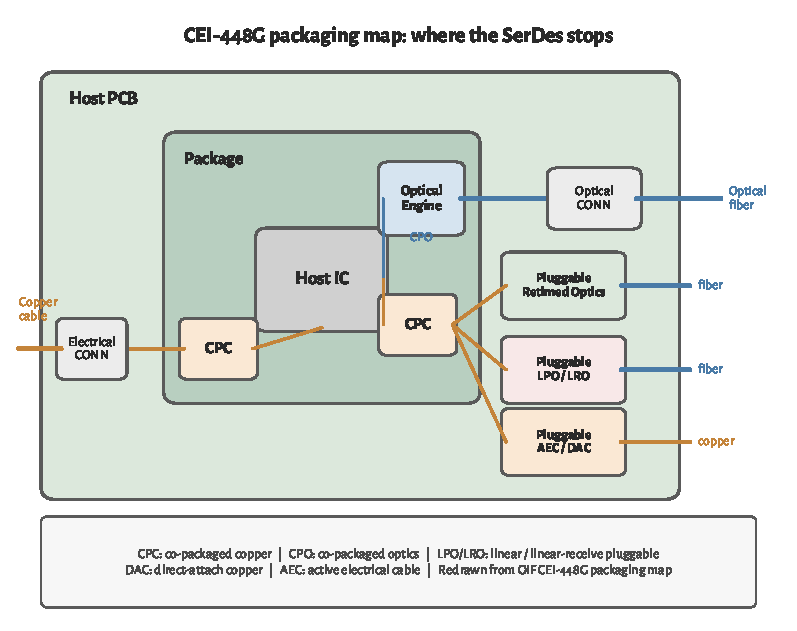
\includegraphics[width=\linewidth]{figures/fig_oif_448g_package.pdf}
\caption{CEI-448G packaging map (redrawn). CPC brings copper to the package edge;
CPO puts an optical engine in the package; faceplate cages take retimed optics,
LPO/LRO, or AEC/DAC. Same host IC, different SerDes reach and EQ burden.
\label{fig:oif-448g-package}}
\end{figure}

\paragraph{What ships today on that map (224G / 200G Ethernet).}
Before the 448G fork, every branch of \Cref{fig:oif-448g-package} already has a
shipping answer at the CEI-224G / IEEE 802.3dj lane rate. Faceplate ports run eight
224~Gb/s PAM4 lanes into 1.6~Tb/s OSFP-class modules (retimed DSP modules still
dominant; LPO and LRO gaining share where host COM and TDECQ close,
\Cref{sec:224g-deploy}). Copper inside the rack uses DAC, ACC, and AEC at the
same SerDes generation. CPO engines shipping with Tomahawk~6 and Quantum-X class
switches are typically \emph{200~Gb/s per optical channel} on 100G/200G SerDes
into microring banks with external lasers (\Cref{sec:cpo-status}): same packaging
map, one generation behind the 448G electrical debate. KP4 FEC, CEI-224G-Linear
for LPO, and KP4 pre-FEC BER near $2.4\times10^{-4}$ are the settled
electrical/optical contract (\Cref{sec:224g,sec:eye-budget,sec:kp4}). The rest of
this section is about what breaks when you try to double that lane rate on the
same shoreline.

So the ``448G debate'' is really two linked questions: can the \emph{electrical}
shoreline run PAM4 at 224~GBd, and can the \emph{optical} \term{PMD} modulate and detect
at the same symbol rate? \Cref{fig:448g-paths} maps the three dominant
architectures and the baud rate at each hop.

\begin{figure}[ht]
\centering
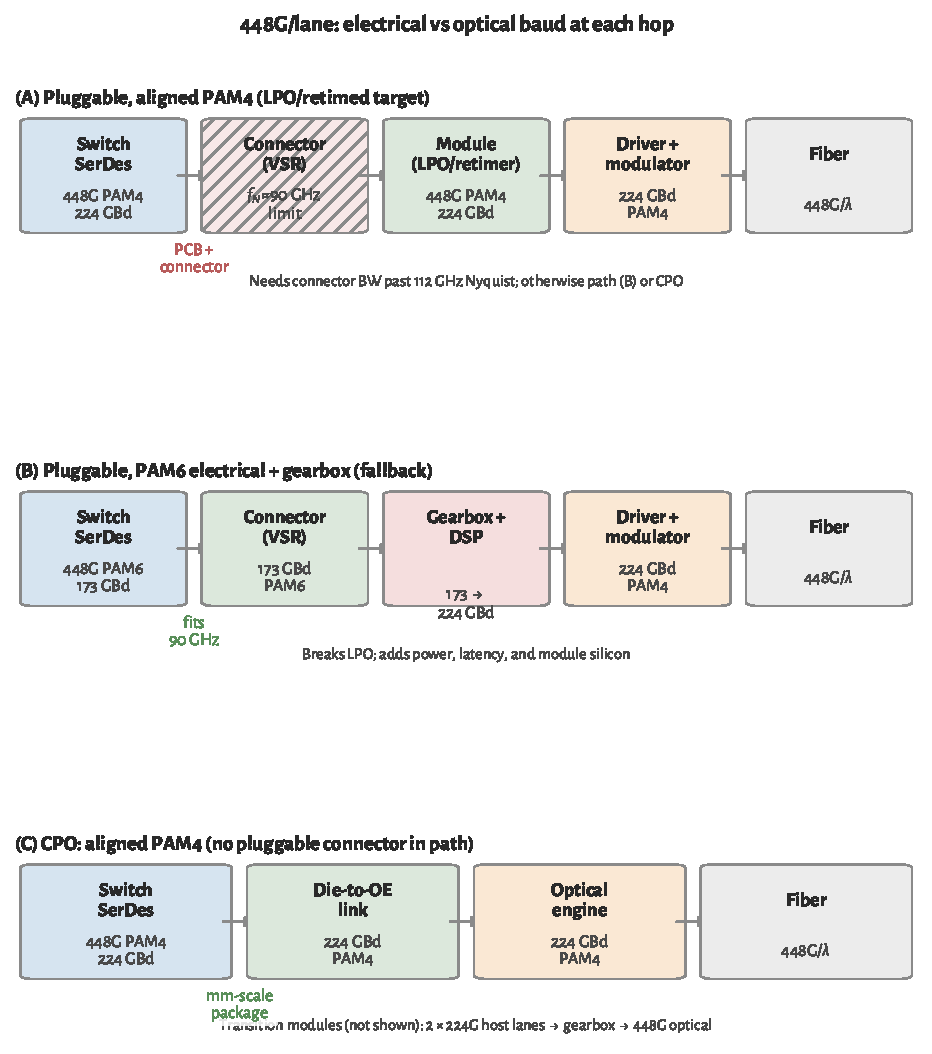
\includegraphics[width=\linewidth]{figures/fig_448g_paths.pdf}
\caption{448G/lane signal paths: aligned pluggable PAM4 (connector-limited),
         PAM6 electrical with module gearbox (LPO incompatible), and CPO or
         gearboxed 224G transition.\label{fig:448g-paths}}
\end{figure}

\begin{table}[ht]
\centering
\caption{PAM-$M$ options at 448~Gb/s/lane (OIF CEI-448G framework, pre-FEC
         line-rate target).\label{tab:448-mod}}
\begin{tabular}{@{}lrrrr@{}}
\toprule
Scheme & Symbol rate & $f_N$ & UI & SNR penalty vs.\ PAM4 \\
\midrule
PAM4 & 224~GBd   & 112~GHz & 4.5~ps & 0~dB \\
PAM6 & 173~GBd   & 87~GHz  & 5.8~ps & $\approx$2~dB \\
PAM8 & 149~GBd   & 75~GHz  & 6.7~ps & $\approx$4--5~dB \\
\bottomrule
\end{tabular}
\end{table}

\paragraph{FEC overhead and the SNR budget.}

At 224G, IEEE and CEI both lean on \term{KP4} FEC: Reed--Solomon RS(544,514) from
802.3 Clause~91, with coding overhead $30/544\approx5.5\%$ and a pre-FEC BER
target near $2.4\times10^{-4}$ for optical PHYs~\firstcite{ieee8023dj,cei448}. Post-FEC
the corrected BER target is $10^{-15}$ class. The line rate on the wire is higher
than the MAC/info rate: a 200~Gb/s Ethernet lane (802.3dj) runs PAM4 at 112~GBd
($224$~Gb/s raw) and delivers $\approx$211~Gb/s of payload after KP4, rounded to
200~Gb/s at the MAC.

448G pushes FEC harder. CEI-448G lists pre-FEC BER $10^{-4}$ as the working target
(same as prior CEI generations) but notes that $10^{-4}$ at $\ge$40~dB channel loss
may not close without a \emph{stronger} code than KP4~\firstcite{cei448}. PAM6 adds
$\sim$2~dB SNR penalty on top, so workshop assumptions often pair PAM6 with
\term{MLC}\firstterm{MLC} and higher-overhead FEC ($\sim$12\%) for a fair comparison to PAM4 with KP4~\firstcite{huawei448}.
\Cref{tab:448-fec} summarizes the landscape (OH\firstterm{OH} = coding overhead); 448G codes are not finalized
(see caption for sources).

\begin{table*}[ht]
\refstepcounter{table}\label{tab:448-fec}%
\centering
\setlength{\tabcolsep}{5pt}%
\begin{tabular}{@{}p{0.19\linewidth}p{0.15\linewidth}p{0.08\linewidth}p{0.49\linewidth}@{}}
\toprule
Context & FEC & OH & Role at 448G/lane \\
\midrule
802.3dj / 224G & KP4 RS(544,514) & 5.5\% &
  Baseline; pre-FEC BER near 2.4e-4. \\
CEI-448G, PAM4 elec. & KP4 or stronger & 5.5\%+ &
  Target pre-FEC 1e-4; KP4 may fail on 40~dB-class channels. \\
CEI-448G, PAM6 elec. & MLC + strong RS & 12\% &
  Offsets PAM6 SNR penalty; adds latency (workshop assumption). \\
448G optical demos & HD-FEC / product & 10--15\% &
  3.2T TFLN demo threshold; not necessarily host FEC. \\
FEC architecture & end-to-end vs.\ terminated & n/a &
  448G may need dedicated electrical inner code. \\
\bottomrule
\end{tabular}
\par\medskip
{\raggedright\footnotesize\textbf{Table~\thetable.} FEC at 448G/lane (448G codes provisional).\par}
\end{table*}
Sources: 802.3dj/KP4 baseline~\firstcite{ieee8023dj}; CEI-448G electrical
targets ~\firstcite{cei448}; PAM6 FEC assumption~\firstcite{huawei448}; optical
\firstterm{HDFEC} demo~\firstcite{tfmln32t}.

Higher FEC overhead feeds back into the modulation debate: every extra parity bit
raises the line rate and Nyquist frequency, which hurts a bandwidth-limited copper
channel. That is one reason PAM6 (lower baud) and stronger FEC get paired, and why
CPO (shorter electrical path) keeps PAM4 attractive.

\paragraph{Electrical SerDes: feasible, but the channel is the gate.}

448G SerDes themselves are widely treated as feasible on advanced CMOS
($\le$N3/N2): ADC/DAC DSP transmitters and receivers demonstrated at 224~Gb/s are
the template, and coherent-optics SerDes with $\sim$100~GHz class AFE at 200~GBd
is cited as encouraging precedent for doubling to 448G-PAM4~\firstcite{cei448}. Synopsys
and others have published channel simulations showing margin for both PAM4 and PAM6
on 224G-class channels when equalization and FEC scale with the modulation
order~\firstcite{synopsys448}. Power targets cluster around 0.5--2.5~pJ/bit at 448G,
similar in spirit to 224G scaling.

The blocker is not the PLL or the DAC; it is the \emph{passive channel}. Connector
bandwidth near 90~GHz forces a fork:

\begin{enumerate}
  \item \textbf{Fix the channel for PAM4:} new high-density connectors, shorter
        reach, skip-layer PCBs, cabled-host internal twinax. Simulations show
        passive CPC reach up to $\sim$1.2~m at 448G-PAM4 under optimistic
        connector assumptions~\firstcite{cei448}. This path preserves electrical/optical
        format alignment and keeps LPO/LRO architectures viable (\Cref{ch:networking}).
  \item \textbf{Keep the channel, change modulation:} PAM6 at 173~GBd fits a
        90~GHz channel but adds $\sim$2~dB SNR penalty and pushes the host toward
        stronger FEC than KP4. PAM8 relaxes bandwidth further at $\sim$4--5~dB
        penalty~\firstcite{cei448}.
  \item \textbf{Bypass the bad channel:} co-packaged optics with millimeter-scale
        die-to-OE links. Host 448G-PAM4 SerDes drives the optical engine directly;
        the pluggable connector never sees 224~GBd~\firstcite{cei448}.
\end{enumerate}

If electrical PAM6 wins on the PCB but optics stay at PAM4, the module needs a
\term{gearbox} (rate/format conversion) in the retimed path. That adds power,
latency, and silicon area, and it breaks linear pluggable optics: LPO requires the
host electrical waveform to match what the optical modulator expects~\firstcite{cei448,lpo}.
First 448G optical modules may therefore ship with gearboxed 224G SerDes (two 224G
lanes per 448G optical lane) before native 448G electrical I/O is
ready~\firstcite{huawei448}.

\paragraph{Optical modulation at 224~GBd: hard, but no longer hypothetical.}

On the optics side, the industry assumption is still IM/DD PAM4 at $\approx$224~GBd
for 448~Gb/s per $\lambda$~\firstcite{cei448,tfmln32t}. That requires roughly 112~GHz
class electro-optic bandwidth in the modulator (and comparable photodiode/TIA
bandwidth in the receiver), plus a driver with enough linear swing and RF BW.
By 2025--26 that stack exists in demos and, increasingly, in announced commercial
parts: silicon rings and MZMs with peaking, TFLN MZMs past 100~GHz EO bandwidth,
EMLs still owning volume at 200G/lane, and SiGe drivers / Ge receivers catching up.
The snapshot below is the state of play; device sections later unpack each family.

\begin{itemize}
  \item \textbf{Silicon microring modulators:} resonant, compact modulators for
        dense WDM and CPO (\Cref{sec:siring}). OFC 2026 demos reach 224--416~Gb/s
        PAM4 with inductive peaking~\firstcite{ring224,ring400}.
  \item \textbf{Silicon Mach--Zehnder modulators:} the broadband, non-resonant
        counterpart to microrings (\Cref{sec:simzm}). OFC 2026 demos reach
        400G/lane PAM4 with SiGe drivers~\firstcite{simzm400}.
  \item \textbf{EML:} integrated DFB + EAM remains the default through 200G/lane
        for DR/FR pluggables: one chip, low chirp, mature supply chain.
  \item \textbf{TFLN MZM:} thin-film lithium niobate Mach--Zehnder modulators with
        CW lasers exceed 100~GHz EO bandwidth and are the leading path to native
        224~GBd IM/DD (\Cref{sec:tfln-mzm}). A 3.2~Tb/s system (eight
        $\times$225~GBd PAM4 lanes) with 3~nm CMOS SerDes and TFLN modulators over
        2~km \term{FR8}/\term{DR8}\firstterm{FR8DR8} was reported in 2025~\firstcite{tfmln32t}.
  \item \textbf{Drivers:} commercial modulator drivers with $>$120~GHz RF BW for
        400G PAM4 EML/MZM/TFLN platforms appeared in 2026~\firstcite{macom448}.
  \item \textbf{Receivers:} Ge/Si PIN and APD photodiodes above 100~GHz and 224G
        TIAs exist (\Cref{sec:pd-tia,sec:rxtech}); the receive side is not the long pole relative
        to modulator/driver bandwidth at 448G.
\end{itemize}

\paragraph{Silicon microring and microdisk modulators.}
\label{sec:siring}

A microring modulator (MRM)\firstterm{MRM} wraps a phase-shifter waveguide into a closed loop
coupled to a straight \emph{bus} waveguide. A \emph{microdisk} is the same idea in
disk form: a pillar cavity evanescently coupled to the bus, often with a wider free
spectral range (FSR)\firstterm{FSR} in a smaller footprint. Both are resonant filters as well as
modulators: when the input wavelength sits on resonance, drop-port power is high;
off resonance it is rejected. Data modulation shifts the resonance (carrier
depletion or injection in an embedded pn junction) or detunes the laser relative
to a fixed ring, mapping voltage to intensity at the through or drop port.

The central design trade is \emph{photon lifetime versus bandwidth}. A high-$Q$
ring stores photons longer, which improves modulator efficiency ($V_\pi$) but narrows
the optical passband and creates an electrical bandwidth ceiling through the
RC-limited junction. Coupling strength, ring radius, and whether the device
operates in under-coupled or over-coupled regime set $Q$, extinction, and the
electro-optic (EO) roll-off. That trade does not appear in broadband Mach--Zehnder
modulators (\Cref{sec:simzm}).

Three constraints dominate ring modulator design at 100--400G per $\lambda$.
First, EO bandwidth: the junction RC roll-off is often below the target Nyquist
frequency, so inductive peaking (T-coils on the drive path), optimized detuning
from resonance, and compact RLC co-design extend EO BW without widening the ring
so much that $Q$ collapses~\firstcite{ring224,ring400}. Production CPO rings
target 50--90~GHz; conference demos report 90--110+~GHz with aggressive
peaking~\firstcite{ring224,ring400,ring256}. Second, wavelength alignment: ring
resonance drifts roughly 10~GHz/\textdegree C in silicon, so each $\lambda$ in a
WDM bank needs the laser or the ring tuned onto the modulator resonance
(\Cref{ch:wdm,sec:locking-techniques}). Thermal crosstalk from neighbors shifts
resonances in dense arrays, which is why fleet validation must include corner
temperature and adjacent-channel heating
(\Cref{sec:thermal-xtalk,ch:validation}). Third, optical loss and FSR: ring radius
sets FSR ($\Delta\lambda$ between adjacent resonances). Microdisk and
\emph{Euler} ring layouts widen FSR so more channels fit under one free spectral
range without collisions~\firstcite{ring256}, while residual coupling loss and
on-resonance insertion loss (often 1--3~dB class per modulator) eat link budget.

Integration is where rings win. A single SOI die can pack dozens of ring
modulators and filters for CW-WDM (\Cref{ch:wdm,sec:cwwdm}), each fed by one
wavelength from an external comb or multi-wavelength ELS (\Cref{ch:lasers}). The
photonic engine co-packaged with a switch ASIC (Broadcom Bailly/Davisson, NVIDIA
Quantum-X/Spectrum-X, \Cref{sec:cpo-status}) uses microring modulators at
200~Gb/s per channel today. Fiber count stays low because many $\lambda$ share one
waveguide; area and modulator count scale with WDM order rather than with
faceplate port count.

State of the art in 2025--26 shows how far that peaking path has been pushed.
Inductive and wavelength tuning carried silicon MRMs to 224~Gb/s PAM4 at 90~GHz
EO BW~\firstcite{ring224}. T-coil-peaked designs report 416~Gb/s PAM4
($\approx$208~GBd) with $>$110~GHz 1-dB EO BW and TDECQ 2.88~dB at
1~Vpp~\firstcite{ring400}. Euler microdisk rings show 256~Gb/s PAM4 with
$>$67~GHz EO BW and 3~THz FSR in O-band~\firstcite{ring256}. These are lab and
conference results, but they match the 200G/lane CPO shipping point and probe
448G-class lane rates when paired with sufficient electrical drive.

The platform choice is a packaging and control decision as much as a bandwidth
one. Prefer rings when many $\lambda$ must fit on one PIC and modulator area
dominates: CPO WDM engines, scale-up optical I/O, and any architecture that already
budgets for wavelength locking (\Cref{ch:wdm,ch:networking}). Prefer a silicon MZM
for single-$\lambda$ DR/FR where a flat passband avoids lock loops
(\Cref{sec:simzm}). Prefer TFLN when you need native 224~GBd in a pluggable and
ring thermal control at fleet scale looks harder than hybrid assembly
(\Cref{sec:tfln-mzm}).

\paragraph{Silicon Mach--Zehnder modulators.}
\label{sec:simzm}

Silicon photonics builds the Mach--Zehnder modulator (MZM)\firstterm{MZM} as a push-pull
interferometer on a silicon-on-insulator (SOI)\firstterm{SOI} rib or strip waveguide. Phase
shifters in each arm use \emph{carrier depletion} in an embedded pn junction:
reverse bias pulls carriers out of the waveguide core, lowering refractive index
and shifting optical phase. Intensity modulation comes from recombining the arms
at a 3-dB coupler, so chirp stays low compared with directly modulated lasers
(\Cref{ch:lasers}).

Three constraints mirror every high-speed MZM, but silicon's weak electro-optic
coefficient ($\Delta n$ per volt is far smaller than lithium niobate) sets the
numbers. The optical $S_{21}$ response must span the Nyquist frequency
($\approx$56~GHz at 112~GBd, 112~GHz at 224~GBd); junction capacitance, series
resistance, and traveling-wave electrode (TWE) microwave loss set the roll-off.
Production Si MZMs for 100--200G/lane modules typically quote 70--100+~GHz 3-dB
BW; differential-drive layouts and compact 300-mm platforms report 80--95~GHz
class results~\firstcite{simzmdiff,simzmcompact}. $V_\pi L$ for carrier-depletion
Si is often $\approx$1.5--2.5~V$\cdot$cm, so millimeter-scale devices need
2--4~V peak-to-peak drive at the target baud inside the linear range of a SiGe
or BiCMOS modulator driver (448G-class drivers exceed 120~GHz RF
BW)~\firstcite{macom448}. Unlike resonant rings, an MZM is broadband, so WDM
channels do not fight thermal lock (\Cref{ch:wdm}); the cost is length:
mm-scale shifters and splitters add 2--4~dB on chip, and the device is far larger
than a ring, which matters in dense CPO tiles.

Integration is the main reason Si MZM survives competition from EML and TFLN.
The modulator shares a die with Ge photodiodes, fiber grating couplers or edge
couplers, monitors, and (in WDM products) MUX/de-MUX filters, all in a CMOS
foundry-compatible flow. An external CW DFB or ELS (\Cref{ch:lasers}) couples in
through a spot-size converter; the RF driver is usually a separate die wire-bonded
or 2.5D packaged next to the PIC, the same assembly style as TFLN modules but
without bonding a second optical material stack.

State of the art in 2025--26: Si MZMs are the default modulator in 100G/lane and
200G/lane DR/FR silicon-photonics\firstterm{SiPh} transceivers. Pushing to 400G/lane IM/DD was open
until OFC 2026, when Coherent reported 400~Gb/s PAM4 per lane with a Si MZM and
commercial SiGe driver (2.5~V swing)~\firstcite{simzm400}. The same conference
cycle showed a 500~$\mu$m compact MZM on a 300-mm platform with 94.7~GHz median EO
BW and 2.4~dB on-chip insertion loss~\firstcite{simzmcompact}, and a
differential-drive MZM with 81.8~GHz 3-dB BW with eyes to 100~GBd
PAM8~\firstcite{simzmdiff}. These are lab and conference demos, not shipping
modules, but they close the headline lane-rate gap with ring modulators while
keeping a flat passband that rings only match with tight wavelength control
(\Cref{sec:siring}).

\paragraph{Thin-film lithium niobate Mach--Zehnder modulators.}
\label{sec:tfln-mzm}

\term{TFLN}\firstterm{TFLN} refers to a sub-micrometer slice of lithium niobate bonded to a
silicon or silica handle wafer. Compared with bulk LN, the tight optical mode
confinement shrinks electrode gap and interaction length, which cuts the
half-wave voltage--length product $V_\pi L$ while keeping a wide
\term{electro-optic}\firstterm{EO} (EO) bandwidth. The modulator is a Mach--Zehnder
interferometer (MZM): a \term{Pockels} phase shifter in each arm, driven in
push-pull, converts RF voltage on a \term{traveling-wave electrode}\firstterm{TWE} (TWE) into
intensity at the output coupler.

Three design constraints set whether a TFLN MZM can run at 224~GBd PAM4
($f_N\approx112$~GHz). EO bandwidth, measured as the $S_{21}$ roll-off of optical
response versus RF drive, must clear that Nyquist: production-class devices quote
$\gtrsim$110~GHz 3-dB BW, and research devices with low-$k$ underfill or advanced
TWE layouts extrapolate toward 200+~GHz~\firstcite{tfln390,tfln200mm}.
$V_\pi L\approx1$--2~V$\cdot$cm is typical, so a 5--7~mm device gives
$V_\pi\approx1.5$--2~V that must fit inside the linear swing of a SiGe or InP
driver at 112~GHz class~\firstcite{macom448,tfln224}. Along the TWE, microwave and
optical group indices must match or bandwidth collapses; low-loss underfill,
narrow-gap CPW or co-planar layouts, and transparent conductive oxide (TCO)
electrodes trade insertion loss against efficiency~\firstcite{tfln224,tfln390}.

Demonstrated IM/DD results on TFLN MZMs include 224~Gb/s PAM4 at 108~GHz EO BW
(O-band, $V_\pi L=1.02$~V$\cdot$cm)~\firstcite{tfln224} and 390~Gb/s PAM8 on the
same dual-band chip (extrapolated 220~GHz BW, sub-fJ/bit in lab)~\firstcite{tfln390}.
System-level proof came with eight $\times$225~GBd PAM4 lanes over 2~km using
3~nm SerDes and packaged TFLN modulators~\firstcite{tfmln32t}. Commercial
suppliers (HyperLight, Lumiphase, and foundry lines on 200-mm silicon) now ship
110~GHz-class packaged MZMs aimed at 200--240~GBd signaling~\firstcite{hyperlight110,tfln200mm}.

Integration looks unlike monolithic silicon photonics. A CW DFB or ELS feeds the
TFLN chip through a Si/SiN coupler; the RF driver sits on a separate die,
wire-bonded or flip-chip mounted with matched 50~$\Omega$ lines. Hybrid Si--LN
platforms (silicon waveguides, LN overlay) were demonstrated early for 100G/lane
and remain a template for co-packaged assemblies~\firstcite{he2019}. The laser
is not on the TFLN chip, so alignment, fiber attach, and thermal bias of the MZM
quadrature point become validation items (\Cref{ch:validation}).

\paragraph{EML and the electro-absorption modulator.}
\label{sec:eml-eam}

An \term{EML} integrates a DFB laser with an \term{EAM}\firstterm{EAM}
(electro-absorption modulator) on one InP chip. The EAM is a reverse-biased
absorption region: voltage shifts the band edge (Franz-Keldysh or quantum-confined
Stark effect), attenuating light with far less chirp than direct current modulation
(\Cref{sec:chirp-dispersion}).

EMLs dominate 100G/lane and 200G/lane DR/FR pluggables because they are single-chip,
mature in supply chain, and match $\sim$70--100~GHz class EO bandwidth
(\Cref{tab:tx-modulator}). The design limits that show up in validation are EAM
bias and aging (bias sets extinction and chirp; aging drifts the curve and shows
up as TDECQ/RLM creep, \Cref{ch:validation,ch:reliability}), driver swing (a few
volts inside the linear absorption region; 448G-class EML drivers appeared
alongside MZM drivers in 2026~\firstcite{macom448}), and thermal headroom
(uncooled datacom is standard; slope efficiency and bias must stay in range
across case temperature).

EML wins on cost and integration through 200G/lane. Above that, external modulators
(Si MZM, TFLN, rings with CW laser) chase bandwidth and chirp headroom
(\Cref{sec:simzm,sec:tfln-mzm,sec:siring}).

\paragraph{Modulator drivers: requirements, records, outlook.}
\label{sec:drivers}

Every external modulator (Si MZM, TFLN, ring, EAM) needs an RF path that delivers
enough \emph{linear} swing at the target baud. That path is either a dedicated
SiGe\firstterm{SiGe}/BiCMOS\firstterm{BiCMOS} \emph{modulator driver} die, or (for LPO) the host SerDes itself.
Laser \emph{bias} drivers are a different circuit and a different noise budget
(\Cref{sec:laser-drivers}). Do not share the modulator driver's switching returns
with the CW bias rail.

\paragraph{What the driver must deliver.}
At 224~GBd PAM4 the symbol Nyquist frequency is 112~GHz, so a usable driver is
not just ``fast enough on paper.'' It needs RF bandwidth roughly
$\gtrsim$100--120~GHz (3~dB) with flat gain and low group-delay ripple, output
swing matched to $V_\pi$ or EAM drive (often $\sim$1.5--3~V peak-to-peak,
differential or single-ended, part- and modulator-dependent), linearity good
enough that RLM and TDECQ stay inside the PMD budget when the optical path adds
its own compression (\Cref{sec:tdecq}), and return loss / matching into
50~$\Omega$ (or the designed modulator impedance) so bondwire and package
reflections do not eat the bandwidth you paid for on the die.
Distributed (traveling-wave) SiGe drivers dominate the high-BW niche: many
cascoded gain cells along an artificial transmission line. Lumped drivers win on
area and power at lower baud. Flip-chip bumped die and short wirebonds matter as
much as $f_T$: a 120~GHz die behind a long bond loop is a 70~GHz module.

\paragraph{Record and commercial snapshot (2025--26).}
\Cref{tab:driver-records} separates research demos (often with offline DSP) from
shipping or announced commercial parts aimed at 1.6T/3.2T modules. Commercial
anchors: MACOM's MAOM-025408 MZM and MAOM-022404 EML drivers ($>$120~GHz RF BW,
OFC~2026)~\firstcite{macom448}; Semtech's GN1877/GN1887 224G quad/octal family for
LPO/LRO/CPO across SiPh, InP, and TFLN~\firstcite{semtech224}. Research anchors:
a 130~nm SiGe distributed driver at 105.7~GHz BW and 2.25~V swing running
232~GBd PAM4 into TFLN (offline DSP)~\firstcite{rfic460drv}; OFC~2026 co-designed
engines at 210~GBd / 420~Gb/s PAM4 (TFLN TOSA)~\firstcite{ofc420tosa}, 180~GBd
PAM4 (InP MZM + EML-class driver)~\firstcite{ofc180drv}, and differential
SiGe+TFLN at 140~GBd PAM8 / 1.4~pJ/bit~\firstcite{tflndiffdrv}; plus the Si MZM
postdeadline with a commercial SiGe driver at 400~Gb/s/lane and 2.5~V
swing~\firstcite{simzm400}.

\begin{table*}[ht]
\refstepcounter{table}\label{tab:driver-records}%
\centering
\setlength{\tabcolsep}{3pt}%
\footnotesize
\begin{tabular}{@{}p{0.24\linewidth}p{0.12\linewidth}p{0.14\linewidth}p{0.16\linewidth}p{0.26\linewidth}@{}}
\toprule
Part / paper & Process & RF BW & Rate / swing & Note \\
\midrule
MACOM MAOM-025408 (MZM) & SiGe & $>$120~GHz & 448G-class PAM4 & Commercial; SiPh MZM \\
MACOM MAOM-022404 (EML) & SiGe & $>$120~GHz & 448G-class PAM4 & Commercial; EML / TFLN \\
Semtech GN1877 / GN1887 & --- & 224G-class & 224~Gb/s/lane & Quad/octal; LPO path \\
RFIC 2026 distributed drv & 130~nm SiGe & 105.7~GHz & 232~GBd; 2.25~V & Research; TFLN; offline DSP \\
OFC 2026 Si MZM + SiGe & commercial SiGe & (drv-limited) & 400~Gb/s/lane; 2.5~V & Postdeadline Th4A.4 \\
OFC 2026 TFLN TOSA & co-designed & --- & 210~GBd / 420~Gb/s & Driver+TFLN engine \\
OFC 2026 InP MZM + EML drv & InP + SiGe-class & 76~GHz MZM & 180~GBd PAM4 & Co-packaged engine \\
Nokia/Bell Labs hybrid & SiGe + TFLN & --- & 140~GBd PAM8; 1.4~pJ/bit & Diff.\ drive; low $V_\pi L$ \\
\bottomrule
\end{tabular}
\par\medskip
{\raggedright\footnotesize\textbf{Table~\thetable.} Modulator-driver snapshot (c.~2026).
Commercial rows are vendor announcements (bandwidth/swing as published); research
rows often use offline DSP and short RF interconnects. ``448G-class'' means aimed at
$\sim$400--448~Gb/s/lane PAM4 modules, not a CEI compliance claim. Sources cited in
the paragraph above.\par}
\end{table*}

\paragraph{LPO and the host-as-driver path.}
For \term{LPO}, the host SerDes (or a linear driver in the module with no retimer)
is the modulator driver. Waveform fidelity is end to end: host FFE, connector ISI,
driver/modulator nonlinearity, and TIA all land in TDECQ and pre-FEC BER
(\Cref{sec:equalization,sec:tdecq,sec:conditioning}). That is why linear-optics
driver families (e.g.\ Semtech's 224G set) advertise CEI-224G-Linear host EQ and
tunable swing: the module cannot clean up what the host launches~\citehref{semtech224}{Semtech 224G}.
Retimed modules hide some of this behind DSP; they also burn the watts LPO was
meant to save.

\paragraph{Outlook.}
Driver roadmaps are no longer waiting on papers alone. Commercial 448G-class
parts are shipping as dies: MACOM's $>$120~GHz MZM and EML drivers (OFC 2026) are
the clearest public 400G/lane announcement~\citehref{macom448}{MACOM}, while
research benches already run past 200~GBd on short RF paths. Expect a short
period where optics and drivers lead host SerDes, so gearboxed 224G electrical
into 448G optical remains common (\Cref{sec:gearbox,sec:448g}). The hard problems
are packaging (bondwire, FAU, faceplate connectors), co-design of peaking with
modulator $S_{21}$, and LPO cases where driver linearity and host COM sit beside
TDECQ as first-order validation items (\Cref{sec:com,sec:prod-corners}). After
the driver, the next ceilings are modulator EO bandwidth and the PD/TIA noise
stack (\Cref{sec:simzm,sec:tfln-mzm,sec:siring,sec:pd-tia,sec:rxtech}).

\keyidea{A 448G-class modulator driver is a $>$100~GHz linear SiGe amp with swing
matched to $V_\pi$, not a SerDes pin. Commercial dies now claim $>$120~GHz for
MZM/EML/TFLN; research shows $\sim$230~GBd on co-designed benches. Package and
modulator match set the real ceiling; LPO makes the host the driver.}

\paragraph{Gearboxes: when electrical and optical rates diverge.}
\label{sec:gearbox}

A \term{gearbox}\firstterm{gearbox} converts lane rate or modulation format between
electrical and optical domains. The 448G transition often uses \emph{two} 224G
electrical lanes into one 448G optical lane (\Cref{fig:448g-paths,sec:448g}) when
host SerDes or connectors lag optics.

Gearboxes add power, latency, and silicon area. They also break strict LPO: the host
waveform no longer matches what the optical lane carries, so a retimed or
half-retimed module is required~\firstcite{cei448,lpo}. Expect gearboxed 3.2T modules
before native 448G electrical I/O and matched VSR connectors land in volume.

Putting the platforms side by side, \Cref{tab:tx-modulator} summarizes the trade
space at 100--400G per $\lambda$; \Cref{sec:siring,sec:simzm,sec:tfln-mzm,sec:eml-eam}
expand each path. Through 200G/lane DR, EML still leads on cost and single-chip
integration. Silicon rings and MZMs lead in CPO where area and CMOS fab matter,
with Si MZM preferred for flat single-$\lambda$ DR/FR and rings preferred for dense
WDM. TFLN leads when you need $\gtrsim$100~GHz EO BW with low chirp for native
224~GBd PAM4 in a pluggable or NPO module and silicon cannot close the 112~GHz
Nyquist without heavy peaking.

\begin{table*}[ht]
\refstepcounter{table}\label{tab:tx-modulator}%
\centering
\setlength{\tabcolsep}{4pt}%
\footnotesize
\begin{tabular}{@{}p{0.11\linewidth}p{0.10\linewidth}p{0.14\linewidth}p{0.08\linewidth}p{0.18\linewidth}p{0.33\linewidth}@{}}
\toprule
Platform & EO BW & Per-$\lambda$ demo & Chirp & Integration & Typical use \\
\midrule
Si microring & 90--110~GHz & 224--416~Gb/s PAM4 & low & monolithic SiPh & CPO, WDM \\
Si MZM & 70--100+~GHz & 400~Gb/s PAM4 & low & monolithic SiPh & DR/FR, CPO \\
TFLN MZM & 108--110+~GHz & 224--390~Gb/s PAM4/8 & very low & hybrid + driver die & 400G/lane pluggable, FR \\
EML & 70--100~GHz & 200~Gb/s PAM4 & low & single InP chip & DR/FR to 200G/lane \\
\bottomrule
\end{tabular}
\par\medskip
{\raggedright\footnotesize\textbf{Table~\thetable.} IM/DD transmitter platforms at 100--400G per $\lambda$ (2026 snapshot).\par}
\end{table*}

The honest summary: \emph{modulating} at 224~GBd PAM4 is demonstrated in multiple
material systems when the electrical drive path is short and the driver is
dedicated (not a lossy meter of PCB plus OSFP connector). \emph{Modulating} at that
rate from a switch ASIC through a pluggable module is the harder system problem.
Silicon photonics rings without peaking still sit below the 112~GHz Nyquist needed
for 448G-PAM4; TFLN, EML, and peaked Si rings are the near-term paths. WDM
(\Cref{ch:wdm}) and CPO remain the architectural escape hatches: more
aggregate bits without forcing every electrical lane to 224~GBd on a lossy
shoreline.

\paragraph{Where the standards conversation stands.}
Electrical and Ethernet standards are climbing the same ladder on slightly
different clocks. OIF CEI owns the electrical I/O recipe; IEEE 802.3 owns how
Ethernet names the lane and the optical PMD. Neither has locked 448G modulation
yet.

\paragraph{OIF CEI (electrical I/O).}
No modulation order is locked yet in CEI-448G. PAM4 remains attractive if
connectors reach $\gtrsim$112~GHz and if optics stay on PAM4 (alignment for LPO,
lower FEC overhead, backward compatibility with 224G gear). PAM6 is the leading
compromise for bandwidth-starved host channels if connector progress
stalls~\firstcite{cei448,cignal448}. Electrical IAs target a 2026--28
window~\firstcite{cei448}.

\paragraph{IEEE 802.3 (Ethernet PHY/MAC).}
Ethernet standards trail CEI slightly but follow the same lane-doubling cadence.
\Cref{tab:ieee-lane} is the map as of mid-2026.

\begin{table}[ht]
\centering
\caption{IEEE 802.3 lane-rate generations.\label{tab:ieee-lane}}
\begin{tabular}{@{}llll@{}}
\toprule
Project & Status & Eth.\ lane & PHY line \\
\midrule
802.3df & Feb 2024 & 100~Gb/s & $\approx$112G PAM4 \\
802.3dj & SA ballot 2026 & 200~Gb/s & $\approx$224G PAM4 \\
802.3 400G/lane SG & Mar 2026 & 400~Gb/s & $\approx$448G \\
\bottomrule
\end{tabular}
\end{table}

\textbf{802.3df} (approved February 2024) defined 200/400/800~Gb/s Ethernet using
\textbf{100~Gb/s lanes} (112~GBd PAM4 class). \textbf{802.3dj} is the active
200~Gb/s-lane amendment: 200/400/800/1600~Gb/s Ethernet with PAM4 at 112~GBd,
KP4 FEC, and a large PHY portfolio (copper and IM/DD optics). The draft cleared
802.3 working-group recirculation ballot in February 2026 and entered IEEE
Standards Association ballot; approval is expected around late
2026~\firstcite{ieee8023dj,e4ai448}.

\textbf{400~Gb/s per lane} is the next Ethernet milestone. The \term{Ethernet for
AI} (E4AI) ad hoc incubated demand for 3.2~Tb/s ports and 400G/lane
signaling~\firstcite{e4ai448}. A call for interest in March 2026 led to an IEEE 802.3
\textbf{400~Gb/s/lane Signaling Study Group} (chartered 13 March 2026) to draft a
PAR for electrical interconnects and single-mode fiber reaches up to
500~m~\firstcite{ieee400gpl}. The proposed scope has two tracks: a fast track for
400/800/1600~Gb/s on 400G/lane copper and IM/DD optics (scale-up, intra/inter-rack),
and a follow-on phase for \textbf{3.2~Tb/s} and additional PHYs~\firstcite{e4ai448,ieee400gpl}.
That aligns with OIF CEI-448G and industry 3.2T module work, with one naming
difference: IEEE quotes \textbf{400~Gb/s per lane} (MAC/info rate); CEI quotes
\textbf{448~Gb/s} (line rate including FEC overhead). They refer to the same
generation.

Until native 448G host SerDes and matched connectors land, expect a transition
generation that gearboxes 224G electrical lanes into 448G optical lanes
(\Cref{fig:448g-paths}), then a consolidation generation with 400G/lane Ethernet
PHYs where electrical and optical both run PAM4 at 224~GBd end to end.

\keyidea{IM/DD is intensity in, power out, with FEC and DSP closing the gap that
PAM4's SNR penalty opens. Master OMA, ER, chirp/dispersion, and pre-FEC BER and
you can reason about any short-reach link.}

\chapter{Multilevel Signaling: From PAM4 to PAM8}
\label{ch:multilevel}
\label{ch:pam}

This chapter is the design judgment home for multilevel intensity modulation:
why more levels exist, what you pay in SNR and linearity, how Gray coding
changes the bit-error story, and when PAM8 is or is not worth it. Roadmaps and
per-lane rates live in \Cref{ch:imdd}. Noise and BER math live in
\Cref{ch:models}. Equalizer design lives in \Cref{ch:equalization}.

\textit{Read first:} baud versus bit rate, level spacing, Gray coding, and the
PAM8 pressure list.

\textit{Deep dive:} 448G alphabet options in \Cref{sec:448g,tab:448-mod};
NRZ/PAM4 quantitative comparison in \Cref{sec:nrzpam4}.

\keyidea{PAM8 lowers the baud rate for a given bit rate, but the level spacing
becomes much tighter, so you pay more in SNR, linearity, calibration, and DSP.
Lower baud is purchased with smaller vertical eyes and harder detection.}

\section{Why multilevel signaling exists}
\label{sec:multilevel-why}

A symbol carries information by choosing one of \(M\) amplitudes. The number of
bits per symbol is \(\log_2 M\):

\begin{center}
\footnotesize
\begin{tabular}{@{}lll@{}}
\toprule
Format & Levels \(M\) & Bits per symbol \\
\midrule
NRZ (PAM2) & 2 & 1 \\
PAM4 & 4 & 2 \\
PAM8 & 8 & 3 \\
\bottomrule
\end{tabular}
\end{center}

At a fixed bit rate \(R_b\), the symbol rate (baud) is
\begin{equation}
R_s = \frac{R_b}{\log_2 M}.
\label{eq:baud-vs-bitrate}
\end{equation}

Higher \(M\) lowers the baud for the same throughput. That relaxes the
electrical and optical bandwidth the channel, connectors, driver, modulator,
and receiver must support. The cost is smaller vertical openings between
adjacent levels and stronger sensitivity to noise, distortion, and nonlinearity.

\paragraph{Worked example at 200~Gb/s.}
Using \Cref{eq:baud-vs-bitrate} at \(R_b=200\)~Gb/s (ideal, before FEC
overhead):

\begin{center}
\footnotesize
\begin{tabular}{@{}ll@{}}
\toprule
Format & Ideal symbol rate \\
\midrule
NRZ & 200~GBd \\
PAM4 & 100~GBd \\
PAM8 & \(\approx\)66.7~GBd \\
\bottomrule
\end{tabular}
\end{center}

Real Ethernet and CEI lanes include FEC and coding overhead, so published baud
numbers differ slightly from this ideal (\Cref{tab:pam4-rates,sec:224g}). The
design point is unchanged: multilevel buys baud relief and spends vertical
margin.

\paragraph{What baud relief buys.}
Lower symbol rate moves the Nyquist frequency down. That can mean less channel
loss at the frequency that matters, less connector bandwidth demand, and more
headroom in the driver and modulator electro-optic response. It can also ease
ADC sampling rate when the alphabet is recovered in DSP. None of those gains is
automatic: if the optical path is linearity-limited rather than
bandwidth-limited, denser PAM spends margin without unlocking the link.

\section{Level spacing and noise penalty}
\label{sec:multilevel-spacing}

For equally spaced levels over the same total swing \(A_{\mathrm{total}}\), the
adjacent-level spacing is
\begin{equation}
\Delta = \frac{A_{\mathrm{total}}}{M-1}.
\label{eq:level-spacing}
\end{equation}

NRZ has one eye. PAM4 has three eyes. PAM8 has seven eyes. With the same
full-scale swing:

\begin{itemize}
\item PAM4 adjacent spacing is one-third of the total swing;
\item PAM8 adjacent spacing is one-seventh of the total swing.
\end{itemize}

Relative to NRZ's full swing as one step, the ideal amplitude-separation
comparisons are about \(20\log_{10}3\approx9.5\)~dB for PAM4 and
\(20\log_{10}7\approx16.9\)~dB for PAM8 before bandwidth, coding, and
implementation effects. Those are spacing comparisons, not automatic
sensitivity penalties on a finished link
(\Cref{sec:nrzpam4}).

Tighter spacing raises the SNR needed to keep the same symbol-error rate. It
also tightens linearity: compression that was tolerable on a two-level eye can
crush the inner PAM8 eyes. Noise that was acceptable for NRZ can dominate the
smallest PAM8 openings.

\begin{center}
\footnotesize
\begin{tabular}{@{}llll@{}}
\toprule
Format & Eyes & Adjacent spacing vs outer swing & Ideal vs NRZ step \\
\midrule
NRZ & 1 & 1 & 0~dB \\
PAM4 & 3 & $1/3$ & $\approx9.5$~dB \\
PAM8 & 7 & $1/7$ & $\approx16.9$~dB \\
\bottomrule
\end{tabular}
\end{center}

{\raggedright\footnotesize Ideal amplitude-separation comparison for equal
spacing and equal outer swing, before bandwidth, EQ, coding, and transmitter
quality.\par}

\paragraph{Noise is not the only enemy.}
Additive noise sets one floor. Pattern-dependent ISI, reflections, and
level-dependent noise set others. A format with seven eyes has seven places for
those impairments to land. When you debug a multilevel failure, ask which eye
closed first.

\section{Gray coding}
\label{sec:multilevel-gray}

Adjacent levels are normally Gray coded so that a nearest-level mistake flips
one bit rather than several. That matters because detectors usually err to a
neighbor, not to a random distant level.

Two consequences:

\begin{itemize}
\item Symbol error rate (SER) and bit error rate (BER) are not identical. With
      Gray coding, BER is often near \(\mathrm{SER}/\log_2 M\) when most errors
      are adjacent-level mistakes.
\item Without Gray coding, one symbol error can create multiple bit errors and
      waste FEC budget.
\end{itemize}

When you quote a pre-FEC BER target for PAM4 or PAM8, state whether the model
assumes Gray mapping and adjacent-error dominance.

\section{PAM8 design pressure}
\label{sec:pam8-pressure}

Moving from PAM4 to PAM8 is not ``one more bit for free.'' Design pressure
stacks:

\begin{description}
\item[Decision thresholds] Seven thresholds instead of three. Placement error
      and threshold drift hit more eyes.
\item[Linearity] DAC, driver, and modulator compression must stay small across
      the full swing. Inner eyes die first.
\item[Level placement] Absolute and relative level accuracy matter more. RLM
      thinking for PAM4 becomes an eight-level calibration problem.
\item[ADC and DSP] Higher resolution and more precise equalization; more power
      and latency if the alphabet lives in DSP.
\item[Clock recovery] Lower baud helps bandwidth, but multilevel edges and
      denser eyes make timing recovery less forgiving.
\item[FEC dependence] Stronger coding or higher overhead may be needed to buy
      back the SNR spent on spacing (\Cref{tab:448-mod}).
\item[Production calibration] Thresholds, levels, and temperature corners need
      factory and field procedures that PAM4 already strains.
\end{description}

The interview sentence is simple: PAM8 lowers baud, but you pay in SNR,
linearity, calibration, and DSP.

\section{Optical implementation}
\label{sec:multilevel-optical}

Multilevel light can be generated several ways. The architecture choice sets
linearity, extinction, chirp, and calibration.

\begin{description}
\item[Directly modulated laser (DML)] Simple, but chirp and nonlinear
      \(L\)--\(I\) behavior fight dense eyes. Harder as \(M\) grows
      (\Cref{ch:lasers}).
\item[EML] Better spectral control than a DML for many short-reach lanes; still
      needs linear drive for PAM8.
\item[MZM] Often the linearity workhorse when a CW laser feeds a Mach--Zehnder
      modulator. Bias and swing must stay in a linear region of the transfer
      curve.
\item[Ring modulator] Compact and WDM-friendly; resonance and thermal control
      complicate multilevel calibration.
\item[Segmented or cascaded binary modulators] Binary-weighted optical paths
      can synthesize multilevel amplitude by optical addition rather than one
      highly linear analog swing.
\item[DAC-driven linear modulation] Generate PAM8 electrically, then demand a
      linear optical transfer function from driver through modulator.
\end{description}

Ask where the multilevel alphabet is created:

\begin{enumerate}
\item Electrically, before one modulator (DAC + linear optic);
\item With segmented optical modulation;
\item Through optical addition of binary-weighted paths;
\item Or with DSP/DAC plus a carefully linearized optical response.
\end{enumerate}

Each path moves the hard problem: DAC resolution, optical linearity, path
matching, or thermal control. There is no free PAM8 modulator.

\paragraph{Short-reach shortlist.}
For many DR/FR-class modules the credible PAM8 paths are a linear MZM or EML
with a clean DAC/driver chain, or a segmented optical approach if the product
team can match path delays and weights. Rings remain attractive for WDM density
but need an explicit thermal and resonance-control story before they are a PAM8
default. DMLs are usually the last choice for eight-level eyes unless the reach
and rate are modest.

\section{Metrics interviewers expect}
\label{sec:multilevel-metrics}

\paragraph{Outer OMA.}
For PAM4, outer OMA is \(P_3-P_0\), not an inner-eye span. For PAM8, the outer
span is \(P_7-P_0\). Quoting ``OMA'' without saying outer versus per-eye invites
a wrong budget (\Cref{ch:models,app:measurement-reference}).

\paragraph{Per-eye thinking.}
A passing outer eye does not prove the inner eyes are open. Level mismatch,
compression, and ISI hit inner eyes first.

\paragraph{Extinction ratio.}
ER compares high and low optical levels. It is necessary context, not a
substitute for multilevel eye quality.

\paragraph{RLM and level mismatch.}
Relative level mismatch (RLM) for PAM4 asks whether the three eyes are evenly
spaced. PAM8 needs the same idea with more levels: unequal spacing burns SNR
even when outer OMA looks fine.

\paragraph{TDECQ and stressed metrics.}
Transmitter quality metrics after a reference equalizer belong in the
measurement appendix (\Cref{sec:tdecq}). Use them to close a claim; do not treat
a single composite number as a confirmed mechanism.

\section{When PAM8 is not worth it}
\label{sec:pam8-not-worth}

Choose PAM8 only when the baud relief is worth the vertical and linearity cost.

Stay on PAM4 when:

\begin{itemize}
\item the electrical channel already closes at the PAM4 baud with acceptable
      power;
\item the optical path cannot deliver the linearity PAM8 needs;
\item FEC, DSP, or calibration power erases the system gain;
\item production cannot place and hold eight levels across temperature and
      aging.
\end{itemize}

The 448G debate is exactly this trade: fix the channel for higher-baud PAM4, or
accept denser alphabets and stronger coding (\Cref{sec:448g,tab:448-mod}). Do
not treat PAM8 as the default upgrade path.

\section{Interview takeaway}
\label{sec:multilevel-design-review}

\keyidea{I explain multilevel formats as a baud-versus-vertical-margin trade.
I name bits per symbol, level spacing, Gray coding, and where the alphabet is
generated. I do not claim PAM8 is ``more efficient'' without stating the SNR,
linearity, FEC, and calibration bill.}

\section{Interview Q\&A}
\label{sec:multilevel-interview-qa}

Practice aloud. Prefer first-person reasoning. Score with
\Cref{sec:chapter-interview-rubric}.

\paragraph{Question 1. Why use PAM8 instead of staying on PAM4?}
\textit{Tests:} baud relief versus vertical and linearity cost.

\textit{Spoken answer.}
``I use PAM8 when the bit rate forces a PAM4 baud that the channel, connector,
or optics cannot support cleanly. Eight levels cut the ideal symbol rate to
one-third of the bit rate, so Nyquist drops. I only take that deal if the SNR,
linearity, FEC, and calibration budget still close.''

\textit{Pressure follow-up.} ``Is PAM8 always the next step after PAM4?''\\
\textit{Answer pivot.} ``No. If PAM4 already closes, PAM8 mostly buys
complexity.''

\textit{Trap:} ``PAM8 is better because it is higher order modulation.''

\paragraph{Question 2. At the same bit rate, how do NRZ, PAM4, and PAM8 baud
rates compare?}
\textit{Tests:} \(R_s=R_b/\log_2 M\).

\textit{Spoken answer.}
``NRZ uses one bit per symbol, PAM4 two, PAM8 three. At 200~Gb/s ideal, that is
200~GBd, 100~GBd, and about 66.7~GBd. Real lanes add FEC overhead, but the ratio
is the design point.''

\textit{Pressure follow-up.} ``Why do datasheets show different baud numbers?''\\
\textit{Answer pivot.} ``Coding and FEC overhead change the line rate. I still
start from bits per symbol, then apply the standard's overhead.''

\textit{Trap:} treating bit rate and baud as interchangeable for PAM4/PAM8.

\paragraph{Question 3. What SNR penalty does denser PAM create?}
\textit{Tests:} level spacing \(\Delta=A/(M-1)\).

\textit{Spoken answer.}
``For equal spacing over the same total swing, PAM4 adjacent spacing is one
third of the outer swing and PAM8 is one seventh. Ideal amplitude-separation
comparisons are about 9.5~dB and 17~dB versus a full NRZ step before bandwidth
and implementation effects. The practical power penalty also depends on noise
bandwidth, EQ, and FEC'' (\Cref{sec:nrzpam4}).

\textit{Pressure follow-up.} ``Can I quote 9.54~dB as the PAM4 link penalty?''\\
\textit{Answer pivot.} ``Only as the ideal spacing comparison. I would not call
it the finished sensitivity penalty.''

\textit{Trap:} ``PAM8 has no SNR cost because baud is lower.''

\paragraph{Question 4. Why does linearity matter more for PAM8?}
\textit{Tests:} compression and inner-eye collapse.

\textit{Spoken answer.}
``PAM8 has seven eyes. Driver or modulator compression that barely dents PAM4
can close the inner PAM8 eyes. I budget DAC, driver, and modulator linearity
across the full swing, not only the outer levels.''

\textit{Pressure follow-up.} ``Outer OMA looks fine. Why fail?''\\
\textit{Answer pivot.} ``Outer OMA does not prove inner-eye spacing or
linearity.''

\textit{Trap:} ``If average power and outer OMA pass, PAM8 is fine.''

\paragraph{Question 5. How does equalization change for denser PAM?}
\textit{Tests:} EQ handoff without claiming Pass~3 depth.

\textit{Spoken answer.}
``Lower baud can ease channel loss, but denser eyes leave less margin for
residual ISI and noise enhancement. I still need to know whether the impairment
is precursor or postcursor and whether FFE, DFE, or DSP is doing the work
(\Cref{ch:equalization}). PAM8 makes tap precision and adaptation errors more
expensive.''

\textit{Pressure follow-up.} ``Does lower baud remove the need for EQ?''\\
\textit{Answer pivot.} ``No. It can reduce the boost required, but multilevel
links still live or die on residual ISI.''

\textit{Trap:} ``PAM8 needs no equalization because baud is lower.''

\paragraph{Question 6. How does FEC interact with PAM8?}
\textit{Tests:} coding as part of the alphabet trade.

\textit{Spoken answer.}
``Denser PAM often needs stronger FEC or higher overhead to buy back SNR spent
on level spacing. I treat FEC as part of the architecture trade, not as a
cleanup step after the alphabet is chosen'' (\Cref{tab:448-mod}).

\textit{Pressure follow-up.} ``Can FEC fix a nonlinear transmitter?''\\
\textit{Answer pivot.} ``FEC helps random or coded errors within its capability.
It does not repair a closed inner eye from compression.''

\textit{Trap:} ``Pick PAM8 and let FEC handle the rest.''

\paragraph{Question 7. How do you think about threshold calibration?}
\textit{Tests:} seven thresholds and drift.

\textit{Spoken answer.}
``PAM8 needs seven decision thresholds. I ask how they are set at production,
how they track temperature and aging, and what telemetry shows threshold or
level drift. A static room-temperature calibration is not a product argument.''

\textit{Pressure follow-up.} ``Who owns threshold adaptation, optics or DSP?''\\
\textit{Answer pivot.} ``Whoever closes the claim. I name the owner and the
observable used to retune.''

\textit{Trap:} ``Thresholds are set once in the lab.''

\paragraph{Question 8. What is level mismatch, and why does it matter?}
\textit{Tests:} RLM / unequal eyes.

\textit{Spoken answer.}
``Level mismatch means the eyes are not equally spaced. Outer OMA can look
acceptable while an inner eye is starved. For PAM4 we use RLM; for PAM8 I apply
the same idea across eight levels. Unequal spacing burns SNR that the baud
reduction was supposed to buy.''

\textit{Pressure follow-up.} ``Is RLM a mechanism?''\\
\textit{Answer pivot.} ``No. It is a symptom metric. I still find whether the
cause is DAC, driver, modulator, or bias.''

\textit{Trap:} ``RLM is only a PAM4 curiosities checkbox.''

\paragraph{Question 9. What is outer OMA for PAM4 and PAM8?}
\textit{Tests:} outer span versus inner eyes.

\textit{Spoken answer.}
``Outer OMA is the span from the lowest to highest optical level: \(P_3-P_0\)
for PAM4 and \(P_7-P_0\) for PAM8. I never use an inner-eye span as the general
OMA definition in a budget.''

\textit{Pressure follow-up.} ``Does outer OMA replace eye quality metrics?''\\
\textit{Answer pivot.} ``No. It sets the outer swing. Eye quality and level
uniformity still need their own evidence.''

\textit{Trap:} ``OMA means the bottom eye height.''

\paragraph{Question 10. How does extinction ratio fit multilevel links?}
\textit{Tests:} ER versus multilevel quality.

\textit{Spoken answer.}
``Extinction ratio compares high and low levels. It matters for average power,
eye placement, and some noise terms, but it does not by itself prove PAM4 or
PAM8 eye quality. I report ER with outer OMA and level-uniformity evidence.''

\textit{Pressure follow-up.} ``High ER means better PAM8?''\\
\textit{Answer pivot.} ``Not if linearity collapses the inner levels to get that
ER.''

\textit{Trap:} ``Raise ER until PAM8 passes.''

\paragraph{Question 11. How do you choose the optical modulator for PAM8?}
\textit{Tests:} DML/EML/MZM/ring/segmented trade.

\textit{Spoken answer.}
``I ask where the alphabet is generated and which device can stay linear across
eight levels. A DML is usually the hardest for dense PAM. An MZM or segmented
optical approach is often more credible if the electrical DAC and bias control
are solid. Rings need thermal and resonance control in the story
(\Cref{ch:lasers,sec:multilevel-optical}).''

\textit{Pressure follow-up.} ``Can I reuse a PAM4 EML for PAM8?''\\
\textit{Answer pivot.} ``Only if linearity, bandwidth, and calibration evidence
support eight levels, not because the part shipped as PAM4.''

\textit{Trap:} ``Any 224G PAM4 optic is automatically PAM8-capable.''

\paragraph{Question 12. When is PAM8 not worth it?}
\textit{Tests:} stop criteria for denser alphabets.

\textit{Spoken answer.}
``If the channel already closes on PAM4, or if optical linearity, FEC power, or
factory calibration cannot support eight levels, I stay on PAM4 or fix the
channel. Baud relief that spends more power than it saves is a bad trade
(\Cref{sec:pam8-not-worth,sec:448g}).''

\textit{Pressure follow-up.} ``Marketing wants PAM8 on the roadmap. What do you
say?''\\
\textit{Answer pivot.} ``I show the baud gain, the SNR and linearity bill, and
the measurement plan. Without those, PAM8 is a slogan.''

\textit{Trap:} ``Always move to the densest PAM the DAC supports.''

\paragraph{Question 13. Give a 60-second multilevel-signaling plan.}
\textit{Tests:} end-to-end whiteboard answer.

\textit{Spoken answer.}
``I start from the bit rate and ask what baud each alphabet requires. I compare
level spacing and the ideal vertical penalty, then ask whether the channel,
connector, and optics can deliver the needed linearity. I choose where PAM is
generated, electrical or optical, name FEC and EQ assumptions, and define outer
OMA, level uniformity, and threshold calibration evidence. I pick PAM8 only when
baud relief outweighs the SNR and calibration cost.''

\textit{Pressure follow-up.} ``What do you measure first on a PAM8 prototype?''\\
\textit{Answer pivot.} ``Outer levels, inner-eye openings or equivalent level
histogram, RLM-class uniformity, and BER or FEC stress at temperature corners.''

\textit{Trap:} ``Look only at average power and a single outer eye.''

\chapter{Quantitative models: noise, RIN, and BER}
\label{ch:models}

The previous chapters argued mostly in architecture and measurement vocabulary.
This one puts numbers behind the two questions every link engineer eventually
asks: \emph{what bit-error ratio (BER) will this receiver deliver?} and
\emph{what is the minimum signal it needs?} The answers follow a short chain of
physics that has been stable for decades of IM/DD design: Gaussian statistics at
the decision circuit, a handful of noise sources, and the way relative intensity
noise (RIN) turns into an error floor. Understanding that chain is what lets you
read a sensitivity number or a RIN floor without treating the datasheet as magic.

Everything here is backed by short, reproducible Python (in \code{sims/}), so the
figures are computed curves rather than sketches. The models follow the treatment
in Säckinger's \emph{Analysis and Design of Transimpedance Amplifiers for Optical
Receivers},\sidenote{\citehref{sackinger2018}{E.~Säckinger, \emph{Analysis and Design of Transimpedance
Amplifiers for Optical Receivers}, Wiley, 2018, ch.~4}.} and the sanity checks in
the code reproduce that book's worked numbers.

\paragraph{Model-fidelity ladder.}
Use the simplest model that answers the decision. Do not force a simple model
to explain evidence outside its assumptions. This is a model-fidelity ladder,
not a product lifecycle.
\begin{description}
\item[Level 1. Scalar link budget] Tx OMA or power, path loss, receiver
      sensitivity, allocated penalties and margin. Answers: does the first-order
      budget close?
\item[Level 2. Equivalent-$Q$ noise model] Optical levels, responsivity,
      thermal/shot/RIN, effective noise bandwidth. Answers: does stochastic
      vertical noise explain the required BER?
\item[Level 3. Waveform and channel model] Finite bandwidth, dispersion,
      jitter, ISI, nonlinear levels, reflections, equalization, compression.
      Answers: how does the real waveform behave?
\item[Level 4. Measured statistical behavior] BER waterfalls, error
      histograms, time-correlated bursts, temperature and lane distributions.
      Answers: does the product population match the model?
\end{description}

\section{The decision: from \texorpdfstring{$Q$}{Q} to BER}
\label{sec:qber}

A binary receiver samples a noisy voltage and compares it to a threshold. If the
noise is Gaussian and the threshold is optimally placed, the BER depends on a
single quality factor $Q$, the separation between the one and zero levels
measured in units of their combined noise:
\[
  Q = \frac{I_1 - I_0}{\sigma_1 + \sigma_0},
  \qquad
  \mathrm{BER} = \tfrac{1}{2}\,\mathrm{erfc}\!\left(\frac{Q}{\sqrt{2}}\right).
\]
The mathematical $Q$-to-BER mapping depends on the sampled level distributions
rather than directly on the optical pulse shape. Pulse shape, bandwidth,
dispersion, jitter, and equalization still determine those distributions and
therefore cannot be ignored when predicting $Q$ from a physical link. This
binary $Q$-to-BER equation is an \emph{equivalent-quality} approximation used
throughout link budgeting. A full PAM4 treatment evaluates three decision
boundaries, unequal level noise, nonlinearity, equalization, and Gray mapping; do
not treat the binary formula as a complete PAM4 model. When applying the
approximation to a PAM4-class example, call it a \emph{binary-equivalent} $Q$.
\sidenote{$Q$ here is the electrical decision quality, not a laser-cavity or
resonator $Q$.} Two reference points anchor the binary curve: the classic uncoded
target $\mathrm{BER}=10^{-12}$ needs $Q=7.03$. For a named KP4-class optical PMD
under its random-error assumption, a pre-FEC objective near $2.4\times10^{-4}$
corresponds to $Q\approx3.5$ on this binary map (\Cref{ch:imdd}). That number is
not a universal Reed--Solomon threshold; state the FEC architecture, error model,
target PMD, and post-FEC metric.

\paragraph{BER and FEC terminology.}
Pre-FEC BER or symbol-error behavior describes the decoder input. Post-FEC
behavior describes residual errors after decoding. Corrected-codeword counts can
reveal declining margin before post-FEC failure. FEC thresholds depend on code,
interleaving, PMD, error distribution, and implementation. Burst errors can be
more harmful than an equal average random BER. A quoted FEC threshold is not a
universal analog receiver specification (\Cref{ch:networking,ch:imdd}).

\begin{lstlisting}
from scipy.special import erfc, erfcinv
import numpy as np

def q_to_ber(q):
    return 0.5 * erfc(q / np.sqrt(2))

def ber_to_q(ber):
    return np.sqrt(2) * erfcinv(2 * ber)
\end{lstlisting}

\begin{figure}[ht]
\centering
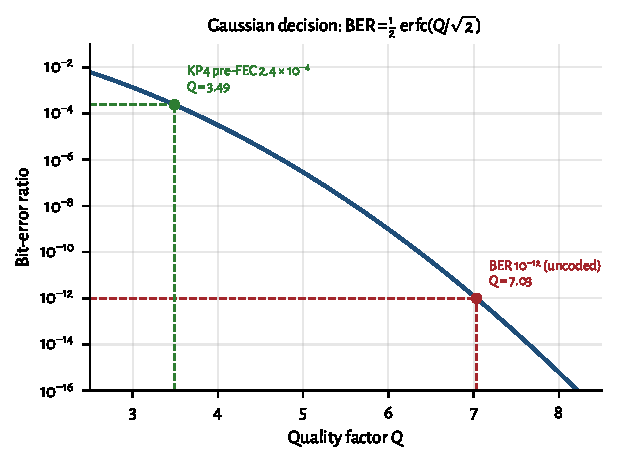
\includegraphics[width=\linewidth]{figures/fig_ber_vs_q.pdf}
\caption{The Gaussian decision curve. Every dB of $Q$ buys orders of magnitude of
BER near the knee, which is why FEC (trading a modest $Q$ for a huge BER
improvement) is decisive.\label{fig:berq}}
\end{figure}

\Cref{fig:berq} shows why the curve is so steep near the operating point: a small
change in $Q$ (equivalently, in received power) moves the BER by orders of
magnitude. This steepness is exactly what FEC exploits: nudging the required $Q$
from 7.03 down to 3.5 relaxes the optical power budget by several dB.

\section{The receiver noise budget}
\label{sec:noise}

$Q$ is only as good as our estimate of $\sigma$. Three noise sources dominate a
short-reach IM/DD receiver. Independent noise sources add in variance (equivalently,
rms amplitudes add in quadrature):

\begin{description}
\item[Thermal / circuit noise] the input-referred noise of the TIA and following
      stages, roughly white, so its variance scales with the noise bandwidth:
      $\sigma_{\text{th}}^2 = i_n'^2\,\mathrm{BW}$, where $i_n'$ is a noise-current
      density (A/$\sqrt{\text{Hz}}$). \emph{Signal-independent.}
\item[Shot noise] from the discreteness of photocurrent,
      $\sigma_{\text{shot}}^2 = 2q\,I\,\mathrm{BW}$. \emph{Grows with signal},
      so it is larger on the ones than the zeros.
\item[RIN (relative intensity noise)] the laser's own intensity fluctuations,
      $\sigma_{\text{RIN}}^2 = \mathrm{RIN}_{\text{lin}}\,I^2\,\mathrm{BW}$, with
      $\mathrm{RIN}_{\text{lin}} = 10^{\mathrm{RIN[dB/Hz]}/10}$.
      \emph{Grows with the square of signal}, the key fact of the next section.
\end{description}

\paragraph{Noise bandwidth.}
Noise bandwidth is the integral of the squared magnitude of the applicable noise
transfer function, expressed as an equivalent rectangular bandwidth. It is not
automatically equal to baud rate, bit rate, or the receiver's quoted $-3$~dB
bandwidth. A first-order estimate must name where the noise density is referred,
which filter response is assumed, and whether equalization changes the integrated
noise.

\paragraph{Limits of variance addition.}
Correlated sources need covariance terms. Discrete spurs should not be treated
automatically as white noise. Data-dependent jitter and ISI are not necessarily
stochastic noise. RIN altered by reflections may be frequency-dependent and
nonstationary. Receiver adaptation can change the effective noise transfer
function. Do not add thermal, shot, and RIN \emph{currents} as if they were
amplitudes on one line.

Because shot and RIN noise are signal dependent, we evaluate $\sigma_1$ and
$\sigma_0$ separately and form $Q$ with their sum. The core of the model is just
this:

\begin{lstlisting}
def nrz_q(p_avg_w, responsivity, i_thermal_rms, bw,
          er_db=np.inf, rin_db_hz=-np.inf):
    p1, p0 = er_levels(p_avg_w, er_db)      # one / zero optical powers
    i1, i0 = responsivity * p1, responsivity * p0
    var1 = i_thermal_rms**2 + 2*Q_E*i1*bw   # thermal + shot
    var0 = i_thermal_rms**2 + 2*Q_E*i0*bw
    if np.isfinite(rin_db_hz):
        rin = 10**(rin_db_hz / 10)
        var1 += rin * i1**2 * bw            # RIN grows as I^2
        var0 += rin * i0**2 * bw
    return (i1 - i0) / (np.sqrt(var1) + np.sqrt(var0))
\end{lstlisting}

\section{RIN and the BER floor}
\label{sec:rin}

Here is the consequence that makes RIN worth its own section. Thermal noise is
fixed, so pouring on more optical power raises $I_1-I_0$ while $\sigma_{\text{th}}$
stays put, so $Q$ improves without limit. But RIN noise scales \emph{with the signal
itself}: $\sigma_{\text{RIN}} \propto I$. Once RIN dominates, the signal and its
noise grow together and $Q$ stops improving. Taking the high-power, high-extinction
limit (thermal and shot negligible, $I_0\to0$):
\[
  Q_{\max} \;=\; \frac{I_1}{\sigma_{\text{RIN},1}}
           \;=\; \frac{1}{\sqrt{\mathrm{RIN}_{\text{lin}}\,\mathrm{BW}}}.
\]
This is a \emph{simplified dominant-RIN ceiling}, not a universal hard limit for
every PAM4 product. It assumes dominant RIN, a defined effective bandwidth,
approximately Gaussian stationary noise, adequate extinction, binary or idealized
level structure, no receiver overload, and no stronger jitter, ISI, reflection,
or nonlinear limitation. Under those assumptions, no amount of transmit power or
receiver sensitivity can push $Q$ past $Q_{\max}$, so a BER floor appears.
Equivalently, the power penalty to hold a target $Q$ is
\[
  \mathrm{PP} = \frac{1}{\sqrt{1 - Q^2\,\mathrm{RIN}_{\text{lin}}\,\mathrm{BW}}},
\]
which diverges as $Q\to Q_{\max}$.

\heuristic{If the waterfall floors, stop raising launch power as the primary
fix. You are buying photons against a non-power-limited impairment.}

\begin{figure}[ht]
\centering
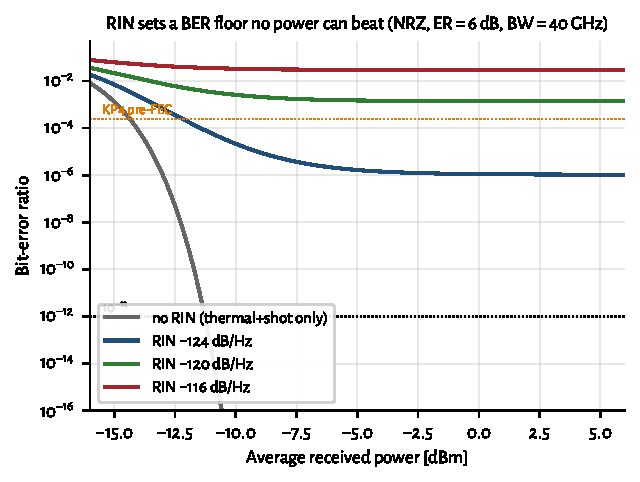
\includegraphics[width=\linewidth]{figures/fig_ber_vs_power_rin.pdf}
\caption{With RIN present, the BER stops falling no matter how much power is added.
The thermal/shot-only curve dives; each RIN level flattens into a floor. (RIN
values here are deliberately high to make the floor visible in-frame; good DFBs at
$<-150$~dB/Hz have no floor at these rates; see text.)\label{fig:berpower}}
\end{figure}

\begin{figure}[ht]
\centering
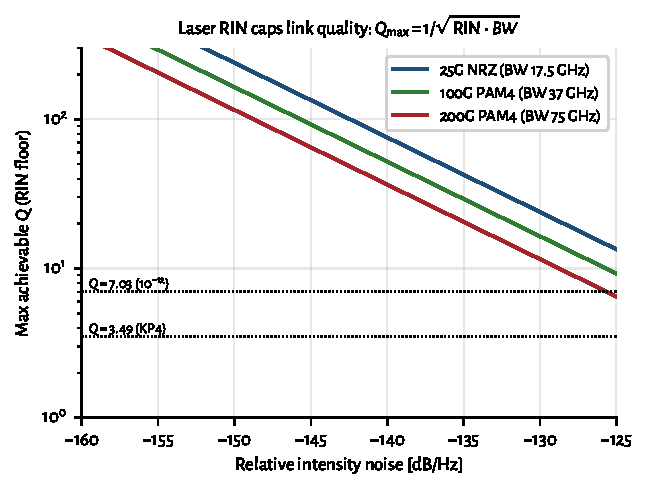
\includegraphics[width=\linewidth]{figures/fig_rin_floor.pdf}
\caption{The RIN ceiling $Q_{\max}=1/\sqrt{\mathrm{RIN}\cdot\mathrm{BW}}$. Wider
receiver bandwidth (higher lane rate) integrates more RIN, lowering the ceiling.
Where a curve dips below the dotted anchors, that link can no longer reach the
corresponding BER.\label{fig:rinfloor}}
\end{figure}

\Cref{fig:berpower} shows the floor directly; \Cref{fig:rinfloor} plots the ceiling
versus RIN for three lane rates. The bandwidth dependence matters: doubling the
lane rate doubles the noise bandwidth and drops $Q_{\max}$ by
$\sqrt{2}$ ($\approx1.5$~dB of margin), so RIN that is harmless at 25G can bite at
200G. This is the quantitative reason the laser chapter (\Cref{ch:lasers}) lists
RIN among the parameters that decide pass/fail.

\subsection{Typical RIN values (2026)}
\label{sec:rin-values}

How much RIN headroom do real sources have? \Cref{tab:rin-values} collects
representative figures. Two cautions on reading them. First, standards quote
\emph{$\mathrm{RIN}_x\mathrm{OMA}$}, RIN referenced to the OMA and measured under
a specified optical return loss (ORL) $x$, because back-reflections into the laser
raise its noise, so a spec limit is a stressed, worst-case number, not the
device's quiet intrinsic RIN.\sidenote{For example \citehref{rinspec}{IEEE~802.3 / 100G~Lambda~MSA
short-reach PAM4 links} cap $\mathrm{RIN}_{17.1}\mathrm{OMA}$ at $-136$~dB/Hz with
\SI{17.1}{dB} ORL~\cite{rinspec}.} Second, RIN degrades with optical feedback, so
isolator-free and co-packaged designs care as much about \emph{feedback tolerance}
as about the isolated number, one reason quantum-dot lasers (near-zero
linewidth-enhancement factor) are attractive for CPO~\cite{qdrin}.

A RIN number in dB/Hz is, by itself, incomplete: because RIN is \emph{relative},
it only becomes an absolute noise current once the photocurrent $I=\mathcal{R}P$
is fixed. The intensity-noise current density is
\[
  i_{\text{RIN}} = \sqrt{\mathrm{RIN}_{\text{lin}}}\;I \quad[\text{A}/\sqrt{\text{Hz}}],
  \qquad
  S_{\text{RIN}} = \mathrm{RIN}_{\text{lin}}\,I^2 \quad[\text{A}^2/\text{Hz}],
\]
so it scales linearly with received power. \Cref{tab:rin-values} therefore lists
both the RIN and the current density it produces at a common reference operating
point ($\mathcal{R}=0.8$~A/W, $P_{\text{rx}}=0$~dBm, i.e.\ $I=0.8$~mA), the units a
receiver designer actually compares against.

\begin{table*}[ht]
\refstepcounter{table}\label{tab:rin-values}%
\centering
\setlength{\tabcolsep}{4pt}%
\renewcommand{\arraystretch}{1.25}%
\begin{tabular}{@{}p{0.26\linewidth}p{0.12\linewidth}p{0.18\linewidth}p{0.12\linewidth}p{0.18\linewidth}@{}}
\toprule
Source & RIN (dB/Hz) & $i_{\text{RIN}}$ @ 0 dBm & Metric & Note \\
\midrule
400G-FR4 / 100G Lambda class limit & $\le -136$ & $\ge 127$ & stressed $\mathrm{RIN}_x\mathrm{OMA}$ & named ORL (e.g.\ 17.1~dB) \\
\addlinespace[1.5em]
Datacom VCSEL, 850~nm (MMF) & $-135$ to $-145$ & $45$ to $142$ & intrinsic & quiet parts $\le\!-145$ \\
\addlinespace[1.5em]
Good datacom DFB / EML & $-145$ to $-155$ & $14$ to $45$ & intrinsic & CPO ELS often target $\le\!-145$ \\
\addlinespace[1.5em]
Quantum-dot laser on Si & $-140$ to $-150$ & $25$ to $80$ & intrinsic & feedback-tolerant class \\
\addlinespace[1.5em]
Heterogeneous / injection-locked Si & $-155$ to $-165$ & $4.5$ to $14$ & intrinsic & high-$Q$ feedback \\
\addlinespace[1.5em]
Lab record (QD + injection lock) & $\sim\!-168$ & $\sim 3.2$ & intrinsic & research \\
\bottomrule
\end{tabular}
\par\medskip
{\raggedright\footnotesize\textbf{Table~\thetable.} Representative RIN by source
(c.~2026) at $\mathcal{R}=0.8$~A/W, $P_{\text{rx}}=0$~dBm ($I=0.8$~mA). Intrinsic
RIN and stressed $\mathrm{RIN}_x\mathrm{OMA}$ are different metrics; do not convert
them through one equation unless the definitions align. Density
$i_{\text{RIN}}=\sqrt{\mathrm{RIN}_{\text{lin}}}\,I$.\par}
\end{table*}

For scale, at that same $0.8$~mA the \emph{shot}-noise density is
$\sqrt{2qI}=16$~pA/$\sqrt{\text{Hz}}$ ($S=2.6\times10^{-22}$~A$^2$/Hz) and a good
high-speed TIA adds roughly $25$~pA/$\sqrt{\text{Hz}}$ of thermal noise. So a VCSEL
at $-140$~dB/Hz ($80$~pA/$\sqrt{\text{Hz}}$) already dominates both, while a
heterogeneous source at $-160$~dB/Hz ($8$~pA/$\sqrt{\text{Hz}}$) is a minor term.
The key asymmetry: thermal noise is fixed and shot grows only as $\sqrt{I}$, but
RIN grows as $I$, so at low received power thermal wins and RIN is irrelevant, and
only above a break-in power (\Cref{fig:noisedensity}) does RIN take over. That is
why quoting a RIN figure without an operating power says little.

\begin{figure}[ht]
\centering
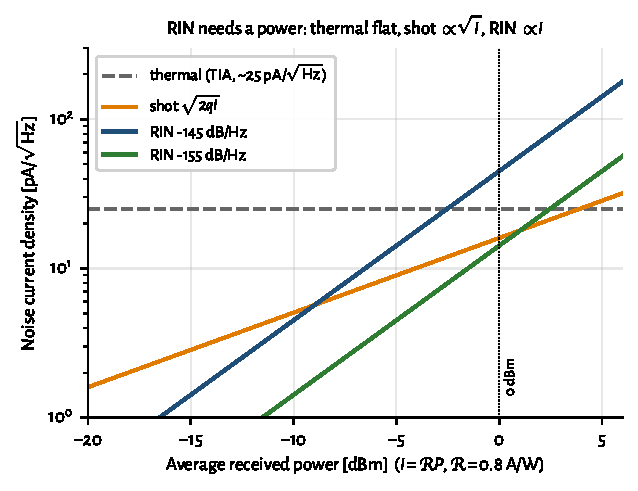
\includegraphics[width=\linewidth]{figures/fig_noise_density_vs_power.pdf}
\caption{Noise current densities versus received power. Thermal is flat, shot
$\propto\!\sqrt{I}$, RIN $\propto\!I$; the RIN curves cross the fixed thermal floor
only above a break-in power, which is why RIN only ``makes sense'' once the optical
power (hence $I=\mathcal{R}P$) is stated.\label{fig:noisedensity}}
\end{figure}

Put these against the simplified dominant-RIN ceiling
$Q_{\max}=1/\sqrt{\mathrm{RIN}\cdot\mathrm{BW}}$. Assumptions: RIN dominates,
noise bandwidth is defined, level structure is idealized, no stronger
deterministic impairment is present, and the receiver is not compressed. At
200G-PAM4 bandwidths ($\mathrm{BW}\approx75$~GHz), plugging the stressed
$-136$~dB/Hz $\mathrm{RIN}_x\mathrm{OMA}$ number into that intrinsic-style formula
is illustrative only; the definitions do not automatically align. Even under that
optimistic plug-in, $Q_{\max}\approx23$ is far above $Q=7$ for $10^{-12}$, so for
well-behaved sources RIN is often not the limiter; thermal noise is. RIN becomes
the story when feedback, aging, or a marginal source pushes the \emph{effective}
intensity noise toward $-125$~dB/Hz class. A third path is electrical: laser
bias-driver current noise converts to equivalent RIN
(\Cref{sec:laser-drivers}) and must be budgeted separately from intrinsic laser
RIN.

\begin{table*}[ht]
\refstepcounter{table}\label{tab:rin-metric-defs}%
\centering
\setlength{\tabcolsep}{3pt}%
\footnotesize
\renewcommand{\arraystretch}{1.2}%
\begin{tabular}{@{}p{0.28\linewidth}p{0.68\linewidth}@{}}
\toprule
Quantity & Meaning \\
\midrule
Intrinsic RIN & Relative intensity-noise spectrum under stated source conditions \\
\addlinespace[0.8em]
Stressed $\mathrm{RIN}_x\mathrm{OMA}$ & Standard-defined Tx metric under a named ORL and normalization \\
\addlinespace[0.8em]
Equivalent bias-board RIN & Optical intensity noise from electrical current-noise coupling \\
\addlinespace[0.8em]
Absolute RIN current density & Current-noise density at a stated photocurrent \\
\bottomrule
\end{tabular}
\par\medskip
{\raggedright\footnotesize\textbf{Table~\thetable.} RIN-related quantities. Similar
units do not guarantee identical definitions
(\Cref{sec:laser-drivers,ch:lasers}).\par}
\end{table*}

\keyidea{Thermal noise is beaten by power; dominant RIN is not. Under a
simplified model, $\sigma_{\text{RIN}}\propto I$ imposes
$Q_{\max}=1/\sqrt{\mathrm{RIN}\cdot\mathrm{BW}}$. Keep intrinsic RIN and stressed
$\mathrm{RIN}_x\mathrm{OMA}$ separate. Feedback, aging, and bias-board noise erode
the margin that quiet intrinsic sources appear to have.}

\section{Sensitivity and OMA}
\label{sec:sensitivity}

\subsection{Common misconception: sensitivity does not guarantee a working link}

Received power exceeding the datasheet sensitivity number does not guarantee low
BER. Sensitivity is measured under specific, controlled assumptions: a clean
transmitter, known extinction ratio, specified ORL, and a particular equalization
state. In the field, BER depends on all of these simultaneously:

\begin{itemize}
\item received optical power;
\item extinction ratio and OMA (not just average power);
\item RIN under the actual ORL;
\item jitter (random and deterministic);
\item ISI from bandwidth limits and dispersion;
\item receiver thermal noise and any TIA compression;
\item equalization state and FEC margin.
\end{itemize}

Sensitivity is therefore a shorthand for receiver noise performance under reference
conditions, not a complete description of whether the link closes. A link that
``has enough power'' can still fail if ER is poor, RIN is elevated, or the
equalizer is saturated. Always close the full link budget
(\Cref{sec:link-budget}), not just the power line.

\begin{table*}[ht]
\refstepcounter{table}\label{tab:metric-planes}%
\centering
\setlength{\tabcolsep}{3pt}%
\footnotesize
\renewcommand{\arraystretch}{1.2}%
\begin{tabular}{@{}p{0.22\linewidth}p{0.74\linewidth}@{}}
\toprule
Quantity & Required condition \\
\midrule
Transmit average power & Named output plane and operating state \\
\addlinespace[0.7em]
Transmit OMA & Named output plane, modulation definition, calibration method \\
\addlinespace[0.7em]
Received power & Receiver optical-input plane \\
\addlinespace[0.7em]
Receiver sensitivity & Average power or OMA; BER/FEC target; Tx condition; wavelength; temperature \\
\addlinespace[0.7em]
RIN & Intrinsic or stressed definition; optical power or OMA; ORL; frequency range \\
\addlinespace[0.7em]
TIA noise & Density or integrated rms; input reference; bandwidth and loading \\
\addlinespace[0.7em]
BER & Pre- or post-FEC; interval; pattern or traffic; lane and direction \\
\bottomrule
\end{tabular}
\par\medskip
{\raggedright\footnotesize\textbf{Table~\thetable.} Metric and reference-plane
checklist. A number without its metric definition and reference plane cannot be
entered safely into the model.\par}
\end{table*}

\tradeoff{Better receiver sensitivity vs receiver complexity}{APD gain, stronger
DSP, deeper equalization, or quieter optics can close a tight budget}{Power,
latency, calibration burden, and reliability of the more complex path}{When the
sensitivity line is the true limiting ledger after Tx and plant are sound}{Improve
the weakest link, not the most visible datasheet metric.}

\subsection{OMA versus average power}

Two links may have identical average optical power but different BER. The reason
is OMA and extinction ratio. At fixed average power $P_\mathrm{avg}$, the OMA
depends on ER through
\[
  \frac{\mathrm{OMA}}{P_\mathrm{avg}}
  = \frac{2(\mathrm{ER}-1)}{\mathrm{ER}+1},
\]
where ER is the linear extinction ratio $P_1/P_0$. A link with 10~dB ER
($\mathrm{ER}_\mathrm{lin}=10$) delivers
$\mathrm{OMA}/P_\mathrm{avg} = 18/11 \approx 1.636$, while 6~dB ER
($\mathrm{ER}_\mathrm{lin}\approx 4$) delivers $6/5 = 1.200$. The difference is
about 1.36~dB of OMA at the same average power. Whether that 1.36~dB matters
depends on where the receiver sits on its BER waterfall: near the sensitivity
cliff a 1~dB OMA change moves BER by orders of magnitude
(\Cref{sec:qber,fig:berpower}), while well above sensitivity the same change is
invisible. The impact also depends on RIN, bandwidth, equalization state, and
TDECQ; ER alone does not set BER.

For PAM4, the relevant quantity is the outer OMA ($P_3 - P_0$), and level spacing
(RLM) matters independently. A transmitter that launches adequate average power but
has compressed inner eyes (poor RLM) will fail TDECQ even though a power meter
reads in-spec. This is why TDECQ, OMA, and RLM are specified together, not average
power alone (\Cref{sec:tdecq}).

\subsection{The sensitivity formula}

Turning the question around (\emph{what is the least power that meets a target
BER?}) gives the sensitivity. Referring the receiver's input noise current
$i_n$ (already integrated rms, not a density) back to the optical input through
the responsivity $\mathcal{R}$:
\[
  P_{\text{sens}} = \frac{Q\,i_n}{\mathcal{R}}
  \qquad\text{(average power)},\qquad
  P_{\text{sens}}^{\text{OMA}} = \frac{2\,Q\,i_n}{\mathcal{R}}.
\]
These simple expressions assume binary signaling, a stated relation between
average power and OMA, high or explicitly handled extinction ratio,
signal-independent effective rms noise for the simplified form, a linear
detector and TIA, no substantial ISI, jitter, compression, or RIN floor, and an
optimal or defined decision threshold. For PAM4, treat the calculation as a
\emph{first-order binary-equivalent estimate}, not a standards-compliance
receiver calculation. A noise density in A/$\sqrt{\mathrm{Hz}}$ must be
integrated through the effective noise bandwidth before it enters these
equations.

Modern short-reach standards specify \term{OMA} rather than average power. For
binary NRZ, $\mathrm{OMA}=P_1-P_0$; for PAM4, outer OMA is $P_3-P_0$. OMA
decouples the sensitivity spec from extinction ratio. As a check, the textbook
example ($i_n = 1~\mu$A, $\mathcal{R}=0.8$~A/W, $\mathrm{BER}=10^{-12}$) gives
$P_{\text{sens}}=7.03\times1~\mu\text{A}/0.8 = 8.8~\mu$W, or $-20.6$~dBm, which
the code reproduces. A finite extinction ratio costs an idealized further
$\mathrm{PP}_\mathrm{dB}=10\log_{10}[(\mathrm{ER}_\mathrm{lin}+1)/(\mathrm{ER}_\mathrm{lin}-1)]$:
$0.87$~dB at 10~dB ER, $2.2$~dB at 6~dB ER. These penalties feed link budgets
(\Cref{ch:imdd}) and TDECQ discussion (\Cref{ch:validation}); do not double-count
TDECQ as an independent penalty if the compliance method already includes it. Do
not convert every impairment into arbitrary dB, mix average-power sensitivity
with OMA penalties, or combine nominal values from one plane with worst-case
values from another as if they were independent.

\paragraph{Worked example: DR4-class budget check.}
\label{sec:worked-budget}

Take a 200G/lane DR-class estimate with Ge-on-Si PIN ($\mathcal{R}=0.9$~A/W), TIA
$i_n=13$~pA/$\sqrt{\text{Hz}}$, noise bandwidth $\approx60$~GHz, and a KP4-class
pre-FEC objective $2.4\times10^{-4}$ mapped to binary $Q\approx3.5$
(\Cref{sec:qber,sec:kp4}). Reference plane: receiver optical input. Assume
Gaussian noise, equalized eye, no compression, and RIN not yet dominant.

Integrated thermal-class noise: $i_n \sqrt{\mathrm{BW}} \approx
13\times10^{-12}\times\sqrt{60\times10^9} \approx 3.2~\mu$A rms. Required OMA
under the binary sensitivity formula:
\[
P_{\text{OMA,sens}} = \frac{2 Q i_n \sqrt{\mathrm{BW}}}{\mathcal{R}}
\approx \frac{2\times3.5\times3.2~\mu\text{A}}{0.9} \approx 25~\mu\text{W}
\approx -16~\text{dBm}.
\]
Illustrative allocations (not a normative budget): $\sim$3~dB TDECQ-class Tx
impairment \emph{or} remaining margin after a TDECQ-based OMA method (not both),
$\sim$2~dB connector/fiber at stated planes, $\sim$2~dB system margin. That lands
near $-9$~dBm class OMA at the receiver input, or roughly $-6$ to $-4$~dBm
launched depending on reach. Parameter sensitivity: $\pm$1~dB in $i_n$ or
$\mathcal{R}$ moves the estimate about 1~dB; a RIN floor or MPI can invalidate
the waterfall entirely.

Where the model stops: unequal PAM4 levels, level-dependent noise, strong ISI,
compressed TIA, correlated RIN, or a different FEC/error model. If measured
sensitivity is worse, bisect RIN, reflections, and ER
(\Cref{sec:link-budget,sec:optical-channel}).

\paragraph{Model-validity checklist.}
Before applying $Q$, $Q_{\max}$, or $P_{\mathrm{sens}}$, ask:
\begin{itemize}
\item Is the noise approximately Gaussian at the decision point?
\item Is the noise bandwidth defined for this measurement?
\item Are PAM4 levels equally spaced (or is RLM budgeted)?
\item Is noise level-dependent (shot/RIN) accounted for?
\item Is the receiver compressed or overloaded?
\item Is residual ISI deterministic rather than noise-like?
\item Is RIN intrinsic, stressed $\mathrm{RIN}_x\mathrm{OMA}$, or bias-board noise?
\item Is the FEC threshold appropriate for this PMD and error model?
\item Is the input metric average power or OMA, and at which reference plane?
\end{itemize}

\begin{dectree}
Measured BER behavior
  |
Gaussian stationary waterfall?
  |-- YES --> equivalent-Q model may be adequate
  |-- NO  --> inspect PAM4 levels, ISI, jitter,
              bursts, reflections, compression,
              adaptation, and non-Gaussian tails
\end{dectree}

\paragraph{Correlating the model with the bench.}
\label{sec:model-to-bench}
A model is validated by prediction across changed conditions, not by fitting one
curve after the fact. Recommended order:
\begin{enumerate}
\item Verify attenuator and power-meter calibration.
\item Establish the optical reference plane.
\item Measure transmitter average power, OMA, ER or RLM, and quality metric.
\item Measure receiver noise or infer an effective value from trusted
      characterization.
\item Sweep received OMA and record BER with sufficient error count or dwell.
\item Fit only physically meaningful parameters.
\item Compare curve crossing, slope, floor, and overload behavior.
\item Repeat across lanes and temperature.
\item Record model uncertainty and measurement uncertainty separately.
\end{enumerate}

\section{Receiver technologies and their noise (2026)}
\label{sec:rxtech}

The sensitivity formula $P_{\text{sens}}=Q\,i_n/\mathcal{R}$ has exactly two
device inputs: the photodiode responsivity $\mathcal{R}$ and the amplifier's
input-referred noise current $i_n$. So ``receiver noise performance'' is really a
statement about the detector--TIA pair. Ge-on-silicon PIN plus a closely
integrated CMOS or SiGe TIA is a common short-reach path because it offers useful
responsivity, bandwidth, and integration. Alternative detectors become attractive
when gain, saturation, wavelength, linearity, or packaging requirements change
(\Cref{sec:pd-tia}).

\paragraph{Photodiodes and transimpedance amplifiers.}
\label{sec:pd-tia}

The photodiode converts photons to photocurrent; the \term{TIA}\firstterm{TIA}
(transimpedance amplifier) converts current to voltage with low input-referred noise.
For PAM4 at 100--224G/lane:

\begin{itemize}
\item \textbf{PIN (Ge-on-Si):}\firstterm{PIN} no internal gain; lowest excess noise; common
      short-reach choice (\Cref{tab:rxtech}). Capacitance at the TIA input dominates
      $i_n$.
\item \textbf{APD}\firstterm{APD}: internal multiplication. Any sensitivity benefit versus
      PIN depends on gain, excess-noise factor, bandwidth, receiver design, and BER
      target; published Ge/Si APD results often cite roughly 5--9~dB under specific
      conditions, not as a universal gain~\cite{apd}.
\item \textbf{UTC/MUTC:}\firstterm{UTC} electron-only transport for $>\!200$~GHz BW and high
      saturation; used when linearity and speed beat raw sensitivity~\cite{utc}.
\end{itemize}

The TIA often embeds \term{CTLE} for LPO (\Cref{sec:equalization,sec:conditioning}):
a fixed high-frequency boost before the host SerDes ADC. Co-packaging PD and TIA
(sub-mm interconnect) is the noise win repeated throughout this book
(\Cref{ch:firstprinciples}).

\paragraph{Why Ge-on-Si is a common mainstream path.} Germanium grown on silicon
absorbs the O- and C-bands, is CMOS-process-compatible, and can be built on the
same PIC as the modulators and couplers. Modern devices reach
$\mathcal{R}\approx0.8$--$1.0$~A/W with dark currents of single-digit to tens of
nA and, in mid-2020s research, $-3$~dB bandwidths beyond 100~GHz (e.g.\ a recessed
Ge/Si PIN at 106~GHz, $0.93$~A/W, $<10$~nA; SiN-coupled lateral Ge $>110$~GHz at
1~mA)~\cite{gesipd}. Monolithic or 3D/flip-chip co-integration keeps the
PD-to-TIA interconnect short, so the input node capacitance stays low. In common
front-end-limited approximations, input-referred noise rises strongly with input
capacitance and required bandwidth; some simplified architectures produce an
approximate $i_n \!\propto\! C\,f^{3/2}$ scaling. Actual scaling depends on TIA
topology, transistor technology, feedback network, detector impedance,
equalization, power, and stability. Short interconnects remain quiet when those
terms cooperate (\Cref{ch:firstprinciples}).

\paragraph{What the TIA must deliver.}
\label{sec:tia-specs}

The TIA is the receive twin of the modulator driver (\Cref{sec:drivers}). At
224~GBd PAM4 you need bandwidth $\gtrsim$50--70~GHz for a 112~GBd Nyquist-class
front-end (often less than the Tx driver BW because the optical channel and
reference receiver already band-limit; LPO pushes for flatter, more linear TIAs),
input-referred noise in the low teens of pA$/\sqrt{\mathrm{Hz}}$ once co-packaged
with a low-$C$ PD, linearity / overload so large OMA and reflections do not crush
PAM4 levels (RLM) or trip AGC into a bad corner, and optional CTLE for LPO/LRO so
the host SerDes sees a usable eye without module DSP
(\Cref{sec:equalization,sec:conditioning}).
In common front-end-limited approximations, noise rises strongly with input
capacitance and bandwidth (sometimes near $i_n \propto C\,f^{3/2}$). That is why
close detector--TIA integration is valuable at 200G+: every millimetre of
bondwire spends noise and bandwidth that FEC cannot recover. Integration is an
engineering trade against repairability and yield, not a universal mandate.

\paragraph{Noise levels you actually budget.}
\Cref{tab:tia-noise} puts the model numbers next to published front-ends. Shot noise
at 0~dBm into $\mathcal{R}=0.8$~A/W is $\sqrt{2qI}\approx16$~pA$/\sqrt{\mathrm{Hz}}$;
a good TIA sits near that floor. Worse $i_n$ or higher $C$ burns sensitivity
linearly via $P_{\mathrm{sens}}=Q\,i_n/\mathcal{R}$ (\Cref{sec:sensitivity}).

\begin{table*}[ht]
\refstepcounter{table}\label{tab:tia-noise}%
\centering
\setlength{\tabcolsep}{3.5pt}%
\footnotesize
\renewcommand{\arraystretch}{1.25}%
\begin{tabular}{@{}p{0.28\linewidth}p{0.18\linewidth}p{0.22\linewidth}p{0.24\linewidth}@{}}
\toprule
Front-end & $i_n$ (pA$/\sqrt{\mathrm{Hz}}$) & BW / rate & Sensitivity note \\
\midrule
Typical ``good'' short-reach TIA (book model) & $\sim$25 & --- & older rule-of-thumb floor \\
\addlinespace[1.5em]
16-nm CMOS + co-pkg PD & 16.9 & 32~GHz / 112G PAM4 & $-8.2$~dBm class \\
\addlinespace[1.5em]
55-nm SiGe $4\times$112~GBd linear TIA & 13.2 & 65~GHz / 224G & $\sim$1.2~pJ/bit \\
\addlinespace[1.5em]
Shot noise @ 0~dBm, $\mathcal{R}=0.8$~A/W & $\approx$16 & --- & physics floor at that power \\
\bottomrule
\end{tabular}
\par\medskip
{\raggedright\footnotesize\textbf{Table~\thetable.} Input-referred TIA noise densities
used in link budgets (c.~2023--26 published front-ends). Integrate $i_n\sqrt{\mathrm{BW}}$
for rms noise before applying $Q$ (\Cref{sec:sensitivity}). Sources in text.\par}
\end{table*}

2026 linear PAM4 front-ends land around $10$--$17$~pA$/\sqrt{\text{Hz}}$: e.g.\
$16.9$~pA$/\sqrt{\text{Hz}}$ at 112G in 16-nm CMOS ($-8.2$~dBm
sensitivity)~\firstcite{tia112} and $13.2$~pA$/\sqrt{\text{Hz}}$ at 224G in
55-nm SiGe BiCMOS (65~GHz BW, 1.2~pJ/bit)~\firstcite{tia224}. Put these in the
model: $i_n\approx13$~pA$/\sqrt{\text{Hz}}$ integrated over $\sim\!60$~GHz is
$\approx3.2~\mu$A rms, giving an NRZ average sensitivity near $-15$~dBm; the PAM4
level penalty lands OMA sensitivities in the $-8$ to $-10$~dBm range these
front-ends report.

\paragraph{Industry snapshot --- mid-2026 (receivers).}
\Cref{tab:rx-records} pairs detectors and TIAs with maturity labels. Commercial
linear-optics TIAs (Semtech GN1834L/DL, GN1838DL) target LPO/LRO/CPO at 224G/lane
with on-chip EQ (production / sampling class). Semtech has also shown 448G-class
PMD ICs (TN14740 TIA) at OFC~2026 demos (vendor demonstration; not a volume
datasheet claim)~\firstcite{semtech224,semtech448demo}. On the detector side,
recessed Ge/Si PINs at 106~GHz / 0.93~A/W~\cite{gesipd}, Ge/Si UMC-APDs at
105~GHz with a published $\sim$9~dB sensitivity gain over PIN at 224/260G PAM4
under that paper's conditions~\firstcite{apd}, waveguide Ge/Si APDs toward
100~GHz at 2~A/W~\firstcite{gesiapd100}, and OFC~2026 Ge-on-Si APDs at 180~GBd
PAM4~\firstcite{ofc360apd} mark the research edge. UTC/MUTC PDs remain the
high-saturation / $>\!200$~GHz niche~\cite{utc}.

\begin{table*}[ht]
\refstepcounter{table}\label{tab:rx-records}%
\centering
\setlength{\tabcolsep}{3pt}%
\footnotesize
\renewcommand{\arraystretch}{1.25}%
\begin{tabular}{@{}p{0.26\linewidth}p{0.14\linewidth}p{0.16\linewidth}p{0.18\linewidth}p{0.18\linewidth}@{}}
\toprule
Part / paper & Type & BW / $i_n$ or $\mathcal{R}$ & Rate / sens. & Note \\
\midrule
Semtech GN1834L/DL / GN1838DL & TIA & 224G-class; linear+EQ & 224~Gb/s/lane & Commercial LPO/CPO family \\
\addlinespace[1.5em]
Semtech TN14740 (demo) & TIA & 448G-class & 448G/lane demo & OFC 2026 booth; provisional \\
\addlinespace[1.5em]
SiGe $4\times$112~GBd TIA & TIA & 65~GHz; 13.2~pA$/\sqrt{\mathrm{Hz}}$ & 224G PAM4 & Research / product-class paper \\
\addlinespace[1.5em]
16-nm CMOS + co-pkg PD & TIA+PD & 16.9~pA$/\sqrt{\mathrm{Hz}}$ & 112G; $-8.2$~dBm & Co-packaged win \\
\addlinespace[1.5em]
Recessed Ge/Si PIN & PD & 106~GHz; 0.93~A/W & 200~GBd-class & $<$10~nA dark \\
\addlinespace[1.5em]
Ge/Si UMC-APD & APD & 105~GHz @ $M\!\approx\!7$ & 224/260G; $-10.9$/$-10.1$~dBm & $\sim$9~dB over PIN (paper conditions) \\
\addlinespace[1.5em]
Ge/Si WG APD (300~mm) & APD & $>$100~GHz; 2~A/W @ 70~GHz & 400G/lane target & 7~V bias class \\
\addlinespace[1.5em]
OFC 2026 Ge-on-Si APD & APD & 70--100~GHz; 1.5--2~A/W & 180~GBd PAM4 & O- and C-band \\
\addlinespace[1.5em]
UTC / MUTC-PD & PD & $>\!110$--200~GHz & high $I_{\mathrm{sat}}$ & Linear / LPO niche \\
\bottomrule
\end{tabular}
\par\medskip
{\raggedright\footnotesize\textbf{Table~\thetable.} Receiver snapshot (c.~2025--26).
Commercial TIA rows are vendor announcements; APD/PIN rows mix production-intent
SiPh with research demos. Sensitivities are as published (FEC threshold varies).\par}
\end{table*}

\paragraph{Reasonable alternatives to Ge PIN + quiet TIA.}
\Cref{tab:rxtech} lays the detector menu out. III-V InGaAs PINs (flip-chipped)
trade monolithic integration for higher power handling and remain common in
discrete modules. Avalanche photodiodes add internal gain that can improve sensitivity when gain,
excess noise, bandwidth, and BER target cooperate (published short-reach results
often land near 5--9~dB under specific conditions) at the cost of bias complexity
and excess noise; device bandwidth above 100~GHz is no longer rare in
research~\cite{apd,gesiapd100,ofc360apd}.
Uni-traveling-carrier (UTC/MUTC) PDs use electron-only transport for very high
saturation current, linearity, and bandwidth ($>\!200$~GHz) but modest
responsivity, a fit for linear/LPO and $>\!200$~GBd analog optics more than for
raw sensitivity~\cite{utc}. SOA\firstterm{SOA}-preamplified receivers bolt optical gain ahead of
the PD for large effective responsivity and reach, but pay in ASE noise figure,
power, and complexity.

\begin{table*}[ht]
\refstepcounter{table}\label{tab:rxtech}%
\centering
\setlength{\tabcolsep}{5pt}%
\footnotesize
\renewcommand{\arraystretch}{1.25}%
\begin{tabular}{@{}p{0.22\linewidth}p{0.13\linewidth}p{0.15\linewidth}p{0.16\linewidth}p{0.21\linewidth}@{}}
\toprule
Detector & $\mathcal{R}$ (A/W) & $-3$~dB BW & Integration & Where it fits \\
\midrule
Ge-on-Si waveguide PIN & $0.8$--$1.0$ & $60$--$>\!100$~GHz & monolithic on SiPh & mainstream short-reach / CPO \\
\addlinespace[1.5em]
III-V InGaAs PIN (flip-chip) & $0.6$--$0.9$ & $60$--$>\!100$~GHz & hybrid / flip-chip & discrete modules, high power \\
\addlinespace[1.5em]
APD (Ge/Si, InP, UMC) & effective $\uparrow$ (gain) & up to $\sim\!100$~GHz+ & hybrid / emerging & power-starved links; gain benefit condition-dependent \\
\addlinespace[1.5em]
UTC / MUTC-PD & $0.1$--$0.8$ & $>\!110$--$200$~GHz & III-V & linear/LPO, $>\!200$~GBd, high saturation \\
\addlinespace[1.5em]
SOA-preamplified PD & effective $\gg\!1$ & $\sim\!50$~GHz & III-V PIC & tight power budgets; adds ASE noise \\
\bottomrule
\end{tabular}
\par\medskip
{\raggedright\footnotesize\textbf{Table~\thetable.} Short-reach receiver detector
options, c.~2026. Ranges span production to recent research; APD/UTC/SOA figures
are effective (with gain) or device-record.\par}
\end{table*}

\paragraph{Outlook.}
Volume short-reach receive commonly stays on PIN + SiGe/CMOS TIA: noise in the
low teens of pA$/\sqrt{\mathrm{Hz}}$ with $>\!100$~GHz Ge PINs is often enough
for DR/FR PAM4 when closely integrated, so the fight is capacitance and yield as
much as detector physics.
Linear optics raises the bar: LPO/LRO need high linearity, on-chip EQ, and
multi-lane density (Semtech's 224G family is the public commercial marker; 448G
TIA demos are still provisional, \Cref{sec:drivers}). APDs are back in the 200G
conversation when several dB of sensitivity gain changes a power-limited plant;
UTC/MUTC matter when the impairment is saturation or $>\!200$~GBd analog fidelity
rather than photons per bit. Bondwire and FAU still set $C$ and BW, which is why
CPO/NPO win on noise for the same reason they win on energy
(\Cref{ch:firstprinciples}).

\keyidea{Receiver performance is $\mathcal{R}$ and $i_n$, with $i_n$ set by PD+TIA
capacitance. Budget $10$--$17$~pA$/\sqrt{\mathrm{Hz}}$ co-packaged TIAs and
$>\!100$~GHz Ge PIN/APD detectors; use APD gain or UTC saturation when the link
demands it. LPO makes TIA linearity as important as raw noise.}

\section{NRZ versus PAM4, at equal bit rate}
\label{sec:nrzpam4}

The 224G-per-lane roadmap (\Cref{ch:imdd}) rides on PAM4, so it is worth seeing
the trade quantitatively. PAM8 and the full multilevel design argument live in
\Cref{ch:multilevel}. At equal bit rate, PAM4 halves the ideal symbol rate
relative to NRZ but divides the available outer modulation span among three eyes.
The resulting link penalty depends on bandwidth, transmitter linearity, level
spacing, level-dependent noise, equalization, coding, and FEC. The figure
$20\log_{10}3 \approx 9.5$~dB is an \emph{ideal vertical level-separation
comparison} before bandwidth and implementation effects. \Cref{fig:pam4} pits the
two at a common 100~Gb/s: PAM4's narrower bandwidth partly offsets its level
penalty, but it still often needs several dB more received power for the same
BER, repaid by relaxing the electrical bandwidth the SerDes and optics must
support. That balance is why many 100G/lane products used NRZ and 200G/lane
products used PAM4.

\begin{figure}[ht]
\centering
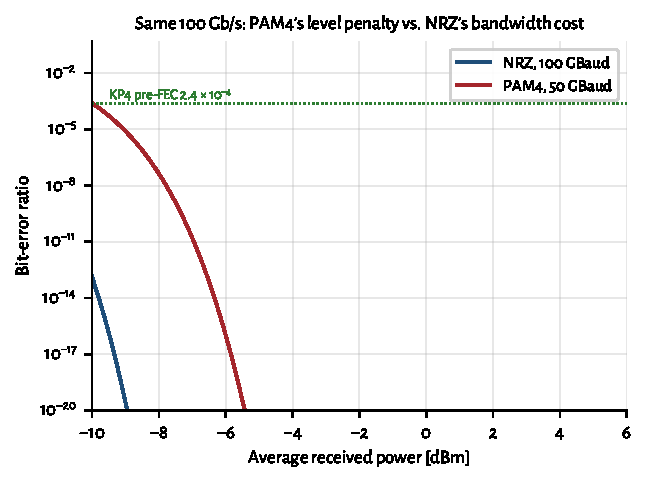
\includegraphics[width=\linewidth]{figures/fig_nrz_vs_pam4.pdf}
\caption{NRZ (100~GBaud) versus PAM4 (50~GBaud) at the same 100~Gb/s. PAM4 pays a
level penalty but relaxes bandwidth; the crossover with the KP4 pre-FEC threshold
sets the required operating power.\label{fig:pam4}}
\end{figure}

\section{Engineering lens}
\label{sec:models-engineering-lens}

\subsection{How it works}

Binary link models often collapse receiver performance to a quality factor $Q$:
signal separation divided by combined noise. That is a useful equivalent-quality
map, not a complete PAM4 theory. Thermal noise yields to more power; dominant RIN
does not, which is why a BER floor can exist. The rest of this chapter computes,
measures, and defends $Q$ under stated assumptions.

\subsection{How it is measured}
\label{sec:models-how-measured}

A BER model earns trust only when every term has a bench measurement. Use a BERT
and calibrated optical attenuator for BER versus received OMA. Measure receiver
input-referred noise with the photodiode dark and illuminated. Use a DCA for OMA,
ER, and eye quality, and a photodiode plus electrical spectrum analyzer for
relative intensity noise (RIN). Repeat power sweeps at temperature and per lane.
Acceptance is a curve, not one point: the required waterfall must cross the
program's pre-FEC threshold with margin and without a floor
(\Cref{sec:qber,sec:noise,sec:rin,sec:sensitivity}).

\subsection{How it fails}
\label{sec:models-how-fails}

Thermal noise dominates at low optical power, shot noise grows with photocurrent,
and RIN grows with signal power. Reflections, crosstalk, jitter, and compression
break a simple Gaussian fit. Curve shape chooses the next experiment; it is not a
root-cause label (\Cref{tab:ber-curve-shape}).

\begin{table*}[ht]
\refstepcounter{table}\label{tab:ber-curve-shape}%
\centering
\setlength{\tabcolsep}{3pt}%
\footnotesize
\renewcommand{\arraystretch}{1.2}%
\begin{tabular}{@{}p{0.22\linewidth}p{0.40\linewidth}p{0.32\linewidth}@{}}
\toprule
Measured behavior & Raises these hypotheses & Does not prove \\
\midrule
Uniform waterfall shift & Lost OMA, loss, greater Rx noise, calibration offset & Which component caused it \\
\addlinespace[0.8em]
High-power floor & RIN, reflections, crosstalk, jitter, bursts, distortion & Intrinsic laser RIN \\
\addlinespace[0.8em]
High-power degradation & TIA/PD overload, compression, AGC/adaptation corner & Excess launch alone \\
\addlinespace[0.8em]
Temperature-dependent shift & Responsivity, noise, OMA, loss, wavelength, EQ & Aging \\
\addlinespace[0.8em]
One-lane-only movement & Lane-local optical or electrical path & Defective laser \\
\addlinespace[0.8em]
Correlated lane movement & Shared rail, source, clock, thermal or control & Common source failure \\
\bottomrule
\end{tabular}
\par\medskip
{\raggedright\footnotesize\textbf{Table~\thetable.} BER-waterfall signatures:
hypothesis routing, not mechanism confirmation
(\Cref{ch:failure-modes}).\par}
\end{table*}

\failuremode{BER floor}{BER improves with received power, then stops improving.}{RIN,
reflection-driven multipath interference, laser-bias noise, crosstalk, or periodic
jitter.}{BER versus OMA, RF RIN spectrum (PD+ESA or RIN analyzer, not OSA), ORL
sweep, FEC error distribution, and a quiet laser-bias source.}{Remove the
correlated noise source, improve ORL, or isolate supplies. The recurrence control
may be source qualification, stressed-RIN screening, supplier process control,
bias-board validation, ORL control, sampled audit, ATP proxy, or fleet monitoring,
depending on where the mechanism can be detected reliably
(\Cref{ch:lasers,ch:reliability,ch:manufacturing}).}

\subsection{How it is debugged}
\label{sec:models-how-debugged}

When pre-FEC BER moves from well below the named FEC threshold into a
$10^{-6}$-class regime, save the failing condition and work in this order:
received OMA, transmitter OMA and ER, receiver noise, RIN and ORL, electrical
jitter, and lane crosstalk.
Sweep power before changing settings. If the curve recovers with power, quantify
the sensitivity shift. If it floors, split intrinsic laser noise from board noise
and reflection feedback. If only temperature moves it, repeat the same terms hot
and cold instead of assigning the change to ``thermal margin.''

\debugstory{One lane developed a BER floor after the product board replaced the
bench supply.}{The optical power sweep flattened. Intrinsic RIN on the quiet
source passed, but discrete tones appeared with the product rails active.}{The
laser was not the noisy element.}{A switching regulator coupled into the laser
bias path.}{The bias filter and return path were changed, and a powered-board RIN
check was added to validation.}

\section{The debugging fork: did received power change?}
\label{sec:debug-fork}

When BER degrades, ask one question first:

\begin{dectree}
BER degraded
  |
Stable average received power?
  |-- NO  --> Power ledger / optical-path investigation
  |           laser / coupling / connector / fiber / MUX / monitor
  |-- YES --> Signal-quality path
              Tx / channel / Rx / DSP
              noise / timing / spectral / control
  |
Highest-value measurement
  |
Decision + recurrence control
\end{dectree}

Stable average received power deprioritizes gross optical loss but does not
clear fast fluctuations, reflections, clipping, wavelength filtering, or
monitor-calibration error. The fork chooses an investigation route; it does not
establish mechanism ownership (\Cref{ch:failure-modes}).

\paragraph{Did average received optical power change?}
If yes, investigate the power path:
\begin{itemize}
\item laser degradation (threshold rise, slope loss, COD);
\item connector contamination or damage;
\item coupling loss (fiber attach, FAU drift);
\item fiber break or bend loss;
\item MUX/de-MUX imbalance or grid misalignment.
\end{itemize}

\paragraph{Or did signal quality degrade at stable average power?}
If average received power is stable but BER worsened, isolate transmitter,
channel, receiver, and DSP quality:
\begin{itemize}
\item noise: RIN (intrinsic, feedback-driven, or bias-driver), Rx noise, crosstalk, MPI;
\item timing: jitter, CDR, skew, adaptation timing;
\item spectral: wavelength, filtering, alignment;
\item control: bias, APC, TEC/heaters, calibration, EQ authority.
\end{itemize}

This fork often narrows an investigation in minutes. Power-path failures show up on
a meter; signal-quality failures need FEC timing, DCA, BERT, or spectrum analysis,
depending on access. Apply it before opening the package, changing settings, or
blaming a supplier
(\Cref{sec:fleet-triage,ch:failure-modes,ch:validation}).

\whyexp{separate power from quality?}{Because average optical power is easy to
measure but tells very little about timing, noise, distortion, or adaptation.
One meter reading prunes an entire branch of the tree.}

\usuallymeans{Stable average power with rising BER}{noise, timing, spectral
alignment, control or calibration, intermittent contact}{gross attenuation as
the primary story}

\section{Interview takeaway}
\label{sec:models-design-review}

\keyidea{Name the metric and reference plane, state the model assumptions, and
close only what the model can defend: Gaussian $\mathrm{BER}(Q)$, the variance
noise budget (thermal + shot + RIN), the simplified dominant-RIN ceiling
$Q_{\max}=1/\sqrt{\mathrm{RIN}\cdot\mathrm{BW}}$, and
$P_{\text{sens}}=Q\,i_n/\mathcal{R}$ with integrated rms noise. Verify with a
measured BER waterfall. Let disagreement reveal missing physics
(\Cref{tab:metric-planes,sec:model-to-bench,tab:ber-curve-shape}).}

Junior mistake: raise launch power into a BER floor, or quote sensitivity without
the measurement conditions (\Cref{sec:rin,sec:debug-fork,ch:lasers,ch:validation}).

\subsection{Interview Q\&A: Quantitative Models, Noise, RIN, and BER}
\label{sec:models-interview-qa}

Practice speaking these answers aloud. Prefer physical meaning and assumptions
over equation recitation. Detail lives earlier in this chapter
(\Cref{sec:qber,sec:noise,sec:rin,sec:sensitivity,sec:debug-fork}).
Score your answer using the chapter-end spoken-answer rubric
(\Cref{sec:chapter-interview-rubric}).

\paragraph{Question 1. What is the $Q$ factor, and when is the $Q$-to-BER
relationship useful?}
\textit{Tests:} physical interpretation, Gaussian assumption, and model scope.

\textit{Spoken answer.}
``In the simple binary receiver model, $Q$ is the separation between the sampled
one and zero levels divided by the sum of their rms noise widths. Under
approximately Gaussian sampled distributions and an appropriate decision
threshold, $Q$ maps to BER through the complementary error function. I use it to
convert measured or modeled signal and noise into an expected error rate and to
understand sensitivity trends. I would not treat it as a complete waveform
model. ISI, non-Gaussian tails, burst errors, unequal PAM4 eyes, clipping, and
adaptation can make the equivalent-$Q$ interpretation incomplete.''

\textit{Pressure follow-up.} ``Can you use the same $Q$ formula directly for
PAM4?''\\
\textit{Answer pivot.} ``Not as a complete PAM4 model. I can use
binary-equivalent-$Q$ approximations for intuition or a stated reference model,
but real PAM4 has three eyes, potentially unequal level spacing, level-dependent
noise, and an FEC-specific error distribution.''

\textit{Trap:} claiming $Q$ completely describes any optical link as long as the
BER is known.

\paragraph{Question 2. Walk me through the receiver noise budget.}
\textit{Tests:} thermal, shot, and RIN scaling.

\textit{Spoken answer.}
``I convert optical levels to photocurrent using detector responsivity, then
calculate the noise at each sampled level. Thermal and circuit noise are
approximately signal-independent and integrate with noise bandwidth. Shot-noise
variance grows linearly with photocurrent. RIN variance grows with the square of
photocurrent. For independent terms, I add variances, not rms amplitudes, and I
calculate the one-level and zero-level noise separately when the noise is
signal-dependent. The resulting level separation and noise widths determine the
equivalent $Q$ and expected BER.''

\textit{Pressure follow-up.} ``Why are $\sigma_1$ and $\sigma_0$ different?''\\
\textit{Answer pivot.} ``Shot noise and RIN depend on photocurrent, so the high
optical level normally has more noise than the low level. Assuming one common
noise value can misplace the optimal threshold and misestimate BER.''

\textit{Trap:} adding thermal, shot, and RIN current amplitudes directly.

\paragraph{Question 3. Why can RIN create a BER floor?}
\textit{Tests:} signal-proportional noise and asymptotic behavior.

\textit{Spoken answer.}
``Thermal noise stays roughly fixed while the signal grows, so more received
power improves signal-to-noise ratio in a thermal-noise-limited link. RIN noise
grows in proportion to the optical signal amplitude, so once RIN dominates,
increasing power increases the signal and its noise together. $Q$ then approaches
a simplified dominant-RIN ceiling and BER stops improving. That ceiling assumes
dominant, approximately white Gaussian RIN, a defined bandwidth, no receiver
compression, and no stronger deterministic impairment.''

\textit{Pressure follow-up.} ``Does a flat BER curve prove intrinsic laser
RIN?''\\
\textit{Answer pivot.} ``No. A floor can also come from optical feedback, MPI,
electrical bias noise, periodic jitter, crosstalk, burst errors, or receiver
limitations. The curve identifies a signal-quality class, not a unique
mechanism.''

\textit{Trap:} treating a BER floor as proof that the receiver needs more
optical power.

\paragraph{Question 4. What can the shape of a BER waterfall tell you?}
\textit{Tests:} shift, floor, shoulder, cliff, and curve interpretation.

\textit{Spoken answer.}
``I compare the complete BER-versus-received-OMA curve rather than one operating
point. A roughly horizontal shift can indicate lost OMA or increased receiver
noise. A high-power floor suggests a signal-proportional, periodic, bursty, or
deterministic impairment. A shoulder or multiple slopes can indicate a change in
dominant mechanism, adaptation behavior, pattern dependence, or mixed
populations. A sharp unexpected cliff may indicate overload, compression,
control saturation, or lock loss. I compare the curve across lanes, temperature,
host, and controlled disturbances before assigning ownership''
(\Cref{tab:ber-curve-shape}).

\textit{Pressure follow-up.} ``Two links have the same sensitivity at the
threshold but different waterfall shapes. Are they equivalent?''\\
\textit{Answer pivot.} ``No. One may have greater margin above the threshold
while the other approaches a floor or cliff. A single crossing point hides the
remaining operating envelope.''

\textit{Trap:} treating the power where BER crosses the FEC threshold as the
only important waterfall result.

\paragraph{Question 5. What must accompany a receiver-sensitivity number?}
\textit{Tests:} reference planes, conditions, and specification interpretation.

\textit{Spoken answer.}
``I need the optical reference plane, whether the metric is average power or
OMA, the modulation format and lane rate, wavelength, transmitter-quality
condition, extinction ratio or level structure, ORL condition, equalization
state, temperature, pattern or traffic condition, FEC and BER criterion, dwell
or error count, and measurement uncertainty. Sensitivity is a receiver result
under defined conditions. It does not independently guarantee that a real
transmitter, fiber plant, and host combination will close''
(\Cref{tab:metric-planes}).

\textit{Pressure follow-up.} ``A supplier says sensitivity is $-10$~dBm. What is
your first question?''\\
\textit{Answer pivot.} ``I would ask whether that is average power or OMA and at
which reference plane and BER or FEC condition. Without those details, the
number is not comparable.''

\textit{Trap:} assuming that if receive power is above the sensitivity number,
the link should work.

\paragraph{Question 6. Explain average optical power, OMA, extinction ratio,
RLM, and TDECQ.}
\textit{Tests:} metric ownership and avoiding composite-metric misuse.

\textit{Spoken answer.}
``Average power measures mean optical energy. OMA measures the modulated optical
separation: one minus zero for NRZ and outer OMA for PAM4. Extinction ratio
describes the ratio of high and low optical levels. RLM describes PAM4
level-spacing linearity. TDECQ is a composite transmitter-quality metric relative
to a defined reference receiver. These metrics answer different questions. Two
transmitters can have the same average power but different OMA or level quality
and therefore very different BER. TDECQ can identify a transmitter-quality
penalty, but it does not identify the physical mechanism.''

\textit{Pressure follow-up.} ``Can you add a TDECQ penalty to a budget that
already uses a TDECQ-based transmitter OMA requirement?''\\
\textit{Answer pivot.} ``Not automatically. That can count the same transmitter
impairment twice. I would first identify exactly what the compliance method and
budget term already include.''

\textit{Trap:} treating OMA, extinction ratio, and TDECQ as different ways of
expressing transmitter power.

\paragraph{Question 7. How do you estimate receiver sensitivity from noise and
responsivity?}
\textit{Tests:} sensitivity model, units, and assumptions.

\textit{Spoken answer.}
``For a simplified binary, thermal-noise-dominated receiver, I integrate the
input-referred noise-current density over the applicable noise bandwidth to
obtain rms current noise. I divide the required signal current by detector
responsivity to refer it to optical power. The required signal separation depends
on the target equivalent $Q$. Before trusting the estimate, I verify whether the
noise value is a density or already integrated, whether the metric is average
power or OMA, whether extinction ratio is finite, and whether shot noise, RIN,
ISI, or compression are important.''

\textit{Pressure follow-up.} ``Why can't you multiply a TIA noise density
directly by $Q$ and divide by responsivity?''\\
\textit{Answer pivot.} ``Because the density has units per square-root hertz. It
must be integrated through the effective noise transfer function, often
approximated as density times the square root of noise bandwidth, before it
becomes rms current.''

\textit{Trap:} using datasheet noise in pA/$\sqrt{\mathrm{Hz}}$ directly in the
optical-sensitivity equation.

\paragraph{Question 8. How do bandwidth and detector--TIA capacitance affect
receiver sensitivity?}
\textit{Tests:} noise-bandwidth tradeoff and integration architecture.

\textit{Spoken answer.}
``Wider electrical bandwidth admits more noise and usually requires a faster
front end with lower impedance or more gain-bandwidth burden. Detector
capacitance, pad capacitance, bond wires, and interconnect parasitics load the
TIA input and make it harder to achieve both low noise and high bandwidth. That
is why close detector--TIA integration is valuable. I would not apply one
universal capacitance-to-noise power law to every topology, but the direction is
clear: excess input capacitance consumes bandwidth, noise, power, or all three.''

\textit{Pressure follow-up.} ``Why not simply narrow the receiver bandwidth to
improve sensitivity?''\\
\textit{Answer pivot.} ``Because insufficient bandwidth creates deterministic ISI
and closes the eye. The optimum bandwidth balances integrated noise against
waveform distortion and equalizer capability.''

\textit{Trap:} claiming maximum receiver bandwidth always provides the best BER.

\paragraph{Question 9. Compare PIN, APD, and high-saturation detector
approaches.}
\textit{Tests:} detector choice and complete receiver tradeoffs.

\textit{Spoken answer.}
``A PIN detector provides no internal gain and is attractive for low excess
noise, simple biasing, and close integration with a TIA. An APD provides
internal multiplication that can improve sensitivity when the gain exceeds the
combined excess-noise and bandwidth penalties, but it adds high-voltage bias,
temperature dependence, gain control, and qualification burden. UTC or MUTC-style
detectors emphasize bandwidth, saturation, and linearity rather than maximum
responsivity. I would choose from the complete detector--TIA requirement:
sensitivity, bandwidth, linearity, overload, power, process integration, yield,
and operating environment.''

\textit{Pressure follow-up.} ``An APD paper reports 8~dB better sensitivity than
a PIN. Does your product receive 8~dB?''\\
\textit{Answer pivot.} ``Not automatically. I would compare modulation, rate, BER
target, gain, bandwidth, noise, reference receiver, temperature, and integration
conditions. Published improvement is conditional, not a universal device
credit.''

\textit{Trap:} claiming an APD is always preferable when the link budget is
tight because it adds optical gain.

\paragraph{Question 10. How do NRZ and PAM4 trade bandwidth against vertical
margin?}
\textit{Tests:} symbol rate, level spacing, and model limitations.

\textit{Spoken answer.}
``At the same bit rate, PAM4 carries two bits per symbol, so its symbol rate is
half that of NRZ and the required channel bandwidth can be lower. The cost is
four amplitude levels and three eyes, so the ideal level spacing is about one
third of the outer OMA before accounting for unequal spacing, level-dependent
noise, and transmitter distortion. That creates a significant vertical-margin
penalty, partly offset by the lower bandwidth and by FEC. I would compare them
using the actual transmitter, channel, receiver, equalization, and FEC model
rather than one universal dB penalty.''

\textit{Pressure follow-up.} ``Why not say PAM4 has exactly a 9.54~dB
penalty?''\\
\textit{Answer pivot.} ``That is the ideal amplitude-separation comparison for
one-third eye spacing. The practical power penalty also depends on noise
bandwidth, coding, level statistics, transmitter quality, and receiver
implementation.''

\textit{Trap:} claiming PAM4 is always more power-efficient because it uses half
the baud rate.

\paragraph{Question 11. The measured BER curve is worse than your model. How do
you reconcile it?}
\textit{Tests:} model correlation and disciplined hypothesis testing.

\textit{Spoken answer.}
``I first verify units, reference planes, OMA calibration, attenuation,
responsivity, noise bandwidth, target BER, and FEC assumptions. Then I compare
the predicted and measured curve shape. A uniform shift may point to
calibration, loss, responsivity, or receiver noise. A floor points toward RIN,
reflections, crosstalk, timing, or bursts. A high-power degradation suggests
compression or overload. I then add one omitted mechanism at a time or run a
measurement that separates the hypotheses. I do not tune several free parameters
until the model matches, because that produces fit without understanding''
(\Cref{sec:model-to-bench}).

\textit{Pressure follow-up.} ``Can you use measured BER to back-calculate
receiver noise?''\\
\textit{Answer pivot.} ``Yes, as an effective parameter under the model
assumptions, but it may absorb transmitter distortion, ISI, and other unmodeled
penalties. I would label it effective noise rather than claim it is the
intrinsic TIA noise.''

\textit{Trap:} adjusting assumed receiver noise until the simulated BER matches
the measurement.

\paragraph{Question 12. Give me a 60-second quantitative link-analysis plan.}
\textit{Tests:} complete Staff-level modeling and measurement answer.

\textit{Spoken answer.}
``I begin by defining the reference planes, modulation format, lane rate, target
BER and FEC, temperature, fiber plant, and required margin. I convert
transmitter levels into received OMA and photocurrent, then build the receiver
noise budget using measured responsivity, input-referred noise, bandwidth, shot
noise, and RIN under the relevant reflection condition. I use an equivalent-$Q$
model only within its assumptions and treat PAM4, ISI, jitter, compression, and
burst behavior separately where needed. I predict the BER waterfall, then
measure it with a calibrated attenuator and compare its crossing, slope, floor,
and temperature movement. The result drives the design margin, architecture
choice, or next discriminating measurement.''

\textit{Pressure follow-up.} ``What evidence would make you reject the
simplified model?''\\
\textit{Answer pivot.} ``Non-Gaussian tails, unequal PAM4 eyes, strong pattern
dependence, a floor unexplained by the included noise, compression, adaptation
discontinuities, or disagreement that cannot be resolved through measurement
uncertainty. At that point I use a waveform, statistical-eye, or
measured-distribution model.''

\textit{Trap:} calculating the link budget, comparing receive power with
sensitivity, and adding a standard margin.

Score each response using the shared chapter-interview rubric in
\Cref{sec:chapter-interview-rubric}. Repeat any answer that does not define the
metric and reference plane, state the model assumptions, connect the model to a
measured curve, and explain what decision the result enables.


\chapter{Choosing light sources and modulation}
\label{ch:lasers}

Do not choose a laser by comparing data sheets in isolation. Start with reach,
lane rate, fiber plant, power, cost, lifetime, manufacturing volume, and service
policy. Those requirements select an architecture. The architecture then limits
the useful source, modulation, detector, packaging, and validation choices.

\section{System requirements and architecture paths}
\label{sec:laser-system-requirements}

Freeze the system problem before asking a supplier for samples:

\begin{dectree}
Reach / fiber plant
  |
Lane rate / bandwidth
  |
Laser choice
  |
Modulator path
  |
Receiver / detector
  |
Validation burden (ATP, lock, thermal, life)
\end{dectree}

\begin{description}
\item[Reach and fiber] decide whether multimode loss and modal bandwidth are
      acceptable or whether the link needs single-mode fiber.
\item[Lane rate and bandwidth] decide whether direct modulation closes the eye or
      whether the link needs an EML, MZM, or ring.
\item[Power and cooling] include laser wall-plug power, modulator loss, driver
      power, TEC power, and control overhead.
\item[Cost and volume] include fiber plant, assembly alignment, burn-in, test time,
      yield, and field replacement, not only die price.
\item[Reliability and service] decide whether the source can stay inside the
      package or must be a replaceable ELSFP.
\end{description}

The choices are coupled. A cost-driven, short multimode link points toward an
850~nm VCSEL, multimode fiber, silicon photodiodes, and direct modulation. A
longer single-mode path points toward a 1310~nm DFB or EML and germanium or
III-V detection. Dense WDM and co-packaged optics often move the CW source away
from the modulator, which adds wavelength control, fiber attach, and service
requirements. \Cref{sec:laser-reqs,tab:laser-req-fork} turns these paths into
supplier specifications.

\section{Light-source and modulation choices}

The short-reach market uses a small set of source families. Each fits a different
constraint set:

\begin{description}
\item[DFB (distributed feedback)] a grating along the active region gives
      single-mode output; the workhorse continuous-wave (CW)\firstterm{CW} or directly
      modulated source for CWDM and LAN-WDM (\Cref{sec:dfb-eml}).
\item[DBR (distributed Bragg reflector)]\firstterm{DBR} the grating sits outside
      the gain region. Choose it when tunability or separate control of gain and
      wavelength is worth added control and qualification work.
\item[External-cavity laser] a gain element and an external wavelength-selective
      cavity provide narrow linewidth and tunability. Choose it when spectral
      purity or lock range matters more than package size, cost, and control-loop
      simplicity. Most short-reach IM/DD links do not need it
      \cite{eclplanex}; the cited product is vendor orientation, not a datacenter
      source recommendation.
\item[DML (directly modulated laser)]\firstterm{DML} modulate the bias current directly: cheap
      and low-power, but chirp-limited over dispersive fiber (\Cref{sec:dml-vcsel}).
\item[EML (externally modulated laser)] \term{EML}\firstterm{EML}: a DFB integrated with an
      \term{EAM}\firstterm{EAM}. Low chirp and high bandwidth make it
      the dominant 100--200G/lane transmitter for single-mode links at DR (500~m)
      and shorter (\Cref{sec:dfb-eml,sec:eml-eam}).
\item[CW laser + TFLN MZM] an external CW source feeds a thin-film lithium
      niobate Mach--Zehnder modulator on a separate chip. Very low chirp and
      $\gtrsim$100~GHz EO bandwidth make this the leading path to 400G/lane
      pluggables and high-baud FR links; see \Cref{sec:tfln-mzm,tab:tx-modulator}.
\item[CW laser + Si MZM] an external CW source feeds a silicon Mach--Zehnder
      modulator on the same PIC (\Cref{sec:simzm}). Low chirp, flat passband, and
      CMOS fab integration make this the default for 100--200G/lane DR/FR SiPh
      modules; 400G/lane demos appeared in 2026.
\item[CW laser + Si ring] same laser architecture, but a microring or microdisk
      modulator on the PIC (\Cref{sec:siring}). Smaller footprint and strong WDM/CPO
      fit; wavelength lock and thermal crosstalk dominate validation (\Cref{ch:wdm}).
\item[CW-WDM / multi-wavelength sources] high-power, multi-wavelength CW lasers
      (per the CW-WDM MSA) that feed comb-like WDM architectures
      (\Cref{sec:cwwdm-laser,sec:cwwdm}).
\item[VCSEL]\firstterm{VCSEL} 850--940~nm multimode sources for short-reach links over multimode
      fiber; cheap but reach-limited and less relevant at 200G/lane.
\item[External laser source (ELS/ELSFP)] a pluggable laser module supplying CW
      light to a co-packaged switch, so a failed laser is field-replaceable
      (\Cref{sec:elsfp}).
\end{description}

\begin{table*}[ht]
\refstepcounter{table}\label{tab:source-mod-matrix}%
\centering
\setlength{\tabcolsep}{2.5pt}%
\scriptsize
\renewcommand{\arraystretch}{1.25}%
\begin{tabular}{@{}p{0.12\linewidth}p{0.13\linewidth}p{0.13\linewidth}p{0.13\linewidth}p{0.13\linewidth}p{0.13\linewidth}p{0.13\linewidth}@{}}
\toprule
Attribute & VCSEL direct & DFB direct & DFB + EAM & CW DFB/DBR + MZM & CW DFB/DBR + ring & External cavity + modulator \\
\midrule
Wavelength / fiber & 850--940~nm / MMF & 1310~nm / SMF & 1310~nm / SMF & 1310 or 1550~nm / SMF & WDM grid / SMF & Tunable grid / SMF \\
\addlinespace[1.5em]
Modulation fit & Direct only & Direct & Integrated EML & Si or TFLN MZM & Resonant Si ring & External MZM or ring \\
\addlinespace[1.5em]
Bandwidth / reach & Short, modal limit & Chirp-limited & High BW, low chirp & High BW, broad passband & High BW, lock-limited & High BW, architecture-specific \\
\addlinespace[1.5em]
RIN / linewidth & RIN and modal noise & RIN and chirp & RIN plus EAM bias & RIN; linewidth usually secondary & RIN plus spectral alignment & Low linewidth; verify feedback response \\
\addlinespace[1.5em]
Power / efficiency & Low Tx complexity & Low Tx complexity & Driver and EAM loss & Laser, driver, and MZM loss & Laser, heater, and lock power & Laser plus control overhead \\
\addlinespace[1.5em]
Reliability & Junction and temperature wear & Facet and active-region wear & Laser plus EAM aging & Source, attach, and bias drift & Source, heater, and lock faults & Cavity, package, and lock faults \\
\addlinespace[1.5em]
Manufacturing & Array-friendly, MMF plant & Simple Tx, SMF attach & Mature integrated Tx & Multi-die attach and RF match & Dense PIC, tight thermal control & Tight optical assembly and control \\
\addlinespace[1.5em]
Validation burden & Modal, temperature, aging & Chirp, LIV, RIN & LIV, RIN, EAM sweep, TDECQ & Source plus bias and RF path & Source plus resonance and crosstalk & Spectrum, lock, feedback, environment \\
\bottomrule
\end{tabular}
\par\medskip
{\raggedright\footnotesize\textbf{Table~\thetable.} Decision matrix for common
source and modulation paths. Entries show the dominant engineering concern, not
fixed rankings. Program limits come from \Cref{tab:laser-prd}.\par}
\end{table*}
\FloatBarrier

\subsection{Reading the source and modulation matrix}
\label{sec:source-mod-matrix-read}

\Cref{tab:source-mod-matrix} is a decision map across paths, not a datasheet.
Read it by \emph{attribute row}: each row asks one engineering question that
every path must answer. Family detail for VCSEL, DML, EML, MZM, and rings
follows in later sections; use this matrix to see which questions become hard
before you commit.

\paragraph{Wavelength / fiber.}

\textbf{Purpose.}
Which wavelength band and fiber type does the path assume?

\textbf{Uncertainty removed.}
Reach, plant, and WDM grid are not free variables after this choice. MMF at
850--940~nm and SMF at 1310/1550~nm pull different connectors, modal limits,
and lock burdens.

\textbf{Decision unlocked.}
Accept the plant class, or reject a path that cannot meet the fiber and grid
requirement.

\textbf{Risk if skipped.}
You pick a modulator before you know whether the link is MMF short-reach or
SMF WDM.

\paragraph{Modulation fit.}

\textbf{Purpose.}
Is the path direct modulation, integrated EAM, external MZM, or resonant
ring?

\textbf{Uncertainty removed.}
Driver, chirp, and lock problems change with the modulator class. Direct
paths buy simplicity and pay chirp or modal limits; external paths buy
bandwidth and pay attach and control.

\textbf{Decision unlocked.}
Allocate driver, bias, and control ownership for the chosen modulator class.

\paragraph{Bandwidth / reach.}

\textbf{Purpose.}
Can the path close the baud and reach without a physics veto?

\textbf{Uncertainty removed.}
Modal bandwidth, chirp, or lock range may kill a path before cost discussions
matter.

\textbf{Decision unlocked.}
Keep the path, derate reach/rate, or move to a higher-BW class (for example
EML or MZM over DML).

\paragraph{RIN / linewidth.}

\textbf{Purpose.}
Which noise and spectral purity limits dominate the BER floor and WDM fit?

\textbf{Uncertainty removed.}
Isolator-free and reflection-rich plants harden RIN. Rings and WDM harden
spectral alignment. External cavities often win linewidth but still need
feedback checks.

\textbf{Decision unlocked.}
Set RIN@ORL and SMSR/linewidth requirements in \Cref{tab:laser-prd}.

\paragraph{Power / efficiency.}

\textbf{Purpose.}
Where does wall-plug and optical power go: laser only, or laser plus driver,
EAM/MZM loss, heaters, and lock?

\textbf{Uncertainty removed.}
``Efficient laser'' claims fail if heater and lock power dominate the module
budget.

\textbf{Decision unlocked.}
Accept the power split, or reject a dense path that breaks the rack power
envelope.

\paragraph{Reliability.}

\textbf{Purpose.}
Which wear-out and fault classes own life: junction, facet, EAM, attach,
heater, or lock?

\textbf{Uncertainty removed.}
Life models and FA paths differ by class (\Cref{sec:wearout-modes}). An
integrated source makes laser yield a package risk; an ELS makes the optical
interface a service risk.

\textbf{Decision unlocked.}
Name the life owner and the screens (HTOL, EAM age, mate cycles) before NPI.

\paragraph{Manufacturing.}

\textbf{Purpose.}
What assembly and plant skills does the path demand?

\textbf{Uncertainty removed.}
Array MMF plants, SMF attach, multi-die RF match, and dense PIC thermal
control are different factories. Path choice is also a supplier-capability
choice.

\textbf{Decision unlocked.}
Pick a path the supply chain can screen, or fund the missing process.

\paragraph{Validation burden.}

\textbf{Purpose.}
Which measurements become mandatory because of the path?

\textbf{Uncertainty removed.}
VCSEL needs modal and temperature work. EML needs LIV, RIN, EAM sweep, and
TDECQ. Rings need resonance, crosstalk, and lock. External cavities need
spectrum, lock, and feedback.

\textbf{Decision unlocked.}
Size the ATP and DVT matrix to the path; do not copy another product's
checklist blindly.

\subsection{How to use the matrix}

\begin{enumerate}
\item Freeze wavelength/fiber and reach/rate from the product requirements.
\item Strike paths that fail bandwidth/reach or plant class.
\item Among survivors, score RIN/linewidth, power, reliability, and
      manufacturing against your constraints.
\item Read the validation-burden row as a cost: every hard cell is an ATP
      and FA investment you must fund.
\item Fill \Cref{tab:laser-prd} from the winning path; reject alternatives
      with a one-line reason retained for review.
\end{enumerate}

Later sections teach each family. Do not let family enthusiasm override a row
that already vetoes the path.

\subsection{Learning summary}

\begin{description}
\item[Wavelength / fiber] Plant and grid first.
\item[Modulation / BW] Physics veto before cost.
\item[RIN / power / reliability] The ledgers that usually decide.
\item[Manufacturing / validation] Can you build and screen it repeatedly?
\end{description}

\section{Directly modulated lasers and VCSELs}
\label{sec:dml-vcsel}

Before EMLs and silicon photonics took over single-mode datacenter ports, most
volume optics were either a cheap \term{DML} on single-mode fiber or a
\term{VCSEL} array into multimode fiber. Both still matter at the low-cost,
short-reach edge of the market, and both show why chirp, modal bandwidth, and
temperature push AI fabrics toward externally modulated single-mode sources.

A DML modulates laser bias current directly. The transmitter is simple and
efficient, but the same carrier dynamics that make modulation easy also produce
chirp: intensity changes drag the optical frequency along
(\Cref{sec:chirp-dispersion}). Over multimode or very short single-mode runs that
is often acceptable. Over dispersive single-mode fiber at tens of GBd, the chirp
turns into inter-symbol interference and closes the eye. Validation therefore
focuses on extinction ratio, pattern-dependent chirp, and RIN, not just average
power.

VCSELs took a different path. They emit from a vertical cavity at 850--940~nm
straight into multimode fiber, so parallel arrays are easy to assemble and cheap
to ship. That combination made VCSEL SR optics the default for early 40G/100G
Ethernet inside the rack (100G-SR4 and its cousins): short ribbons of MMF, high
lane count, low dollars per gigabit. The same physics that made them attractive
also capped their future. Multimode fiber has modal bandwidth and modal noise
limits; VCSEL bandwidth and reliability both degrade with temperature; and as
lane rates climb toward 100~G and 200~G, those limits arrive sooner. The industry
response has been incremental (better OM4/OM5 fiber, tighter specs, sometimes
PAM4 on MMF) rather than a clean leap to 400G/lane SMF DR. In practice, MMF
reach and modal dispersion keep VCSEL links in the SR box
(\Cref{sec:pmd-reach}), while hyperscale AI fabrics standardize on single-mode
DR/FR and CPO.

Neither family is the path to 400G/lane SMF DR. EMLs and external modulators
(\Cref{sec:dfb-eml,sec:simzm,tab:tx-modulator}) own that space. Pattern-aware
chirp linearization can stretch a DML a little farther, but it does not change
the physics at FR distances: if you need low chirp and high EO bandwidth at
fleet scale, you leave direct modulation behind.

\section{DFB and EML: the workhorse transmitters}
\label{sec:dfb-eml}

Once single-mode DR/FR became the hyperscale default, most short-reach ports
started with an InP\firstterm{InP} laser chip. Two configurations still dominate production:
the CW or directly modulated DFB, and the EML that adds an electro-absorption
modulator on the same die.

\paragraph{DFB.} A distributed-feedback laser has a grating along the active region
that selects one longitudinal mode. Spec-sheet metrics that matter in bring-up are
threshold current, slope efficiency, SMSR (typically many tens of dB on a clean
part), RIN, and wavelength vs.\ temperature/current. Used as a CW source for SiPh
or TFLN modulators, or as a DML when chirp is acceptable (\Cref{sec:dml-vcsel}).
Uncooled datacom DFBs ride case temperature with a known $d\lambda/dT$; cooled
parts add a TEC\firstterm{TEC} and lock to a grid.

\paragraph{EML.} An electro-absorption modulated laser integrates a DFB with an
\term{EAM} on one chip (\Cref{sec:eml-eam}). Reverse bias on the EAM sets absorption
and extinction; chirp stays far below a DML. That combination, not marketing, is
why EMLs became the volume answer for 100G/lane and then 200G/lane DR/FR
pluggables: one chip, low chirp, mature supply chain. Validation adds EAM bias
sweeps, aging of the absorption curve, and driver-match checks on top of the DFB
LIV/SMSR/RIN suite (\Cref{sec:laser-params,sec:laser-aging}).

\paragraph{When to pick which.} Through 200G/lane DR, EML usually wins on cost and
integration. A CW DFB (or ELSFP/CW-WDM bank) plus Si MZM, ring, or TFLN wins when
the modulator must sit on silicon or needs $\gtrsim$100~GHz EO bandwidth
(\Cref{tab:tx-modulator,sec:simzm,sec:siring,sec:tfln-mzm}). At CPO scale the laser
often leaves the optical engine entirely so it can be replaced without pulling the
ASIC package (\Cref{sec:elsfp}). Looking forward, 400G/lane pluggables are pushing
harder toward external CW plus TFLN or high-BW silicon modulators, while EMLs
remain the workhorse of the installed 100--200G base.

\begin{table*}[ht]
\refstepcounter{table}\label{tab:laser-choice}%
\centering
\setlength{\tabcolsep}{5pt}%
\renewcommand{\arraystretch}{1.25}%
\begin{tabular}{@{}p{0.14\linewidth}p{0.24\linewidth}p{0.58\linewidth}@{}}
\toprule
Source & Typical use & Top risks \\
\midrule
DML & short reach, cost-driven & chirp/dispersion, extinction ratio \\
\addlinespace[1.5em]
EML & $\le$DR, 100--200G/lane & EAM bias/aging, thermal \\
\addlinespace[1.5em]
CW + TFLN MZM & 400G/lane FR/DR, NPO & MZM bias drift, fiber attach, driver match \\
\addlinespace[1.5em]
CW + Si MZM & DR/FR SiPh, 100--400G/lane & driver match, bias drift, fiber coupling \\
\addlinespace[1.5em]
CW + Si ring & CPO, WDM transceivers & wavelength lock, thermal crosstalk, coupling \\
\addlinespace[1.5em]
VCSEL & SR over MMF & modal noise, reach, temperature \\
\addlinespace[1.5em]
ELS / ELSFP & co-packaged optics & connectorization, fleet serviceability \\
\bottomrule
\end{tabular}
\par\medskip
{\raggedright\footnotesize\textbf{Table~\thetable.} When each source is used, and its top validation risks.\par}
\end{table*}

Use \Cref{tab:laser-choice} as a short risk card once the path is roughly
known. Use \Cref{tab:source-mod-matrix} when you still need to compare
attribute rows across paths. Do not treat this card as a substitute for the
full matrix or for \Cref{tab:laser-prd}.

\section{Choosing the modulation path}
\label{sec:siph-platforms}

The source decision and modulation decision must close together. Direct
modulation minimizes parts and power but carries laser chirp into the link. An
EML adds an EAM on the laser die and is a mature low-chirp path for
100--200G/lane. A silicon MZM uses more area and drive but gives a broad optical
passband. A ring is compact and fits dense WDM, but adds resonance control and
thermal-crosstalk tests. TFLN offers high bandwidth and low chirp with a separate
material platform and assembly flow.

\Cref{tab:source-mod-matrix} compares the system consequences. The device
operation, bandwidth, insertion loss, and driver interfaces live in
\Cref{sec:eml-eam,sec:simzm,sec:siring,sec:tfln-mzm,tab:tx-modulator}. Keep that
physics in one place. Here the decision is whether the link can carry the added
power, control, assembly, and validation burden.

\section{Laser requirements: from roadmap to specs}
\label{sec:laser-reqs}

Laser requirements only work when they are numbers a supplier can fail and a link
budget can close. Start from the interconnect roadmap choice, then fill a short
requirements slice; the ATP in \Cref{sec:supplier-exec} is how that slice is
enforced on every lot.

\paragraph{Roadmap forks that set the laser.}
Each architecture decision forces a different requirements set
(\Cref{tab:laser-req-fork}):

\begin{table*}[ht]
\refstepcounter{table}\label{tab:laser-req-fork}%
\centering
\setlength{\tabcolsep}{3.5pt}%
\footnotesize
\renewcommand{\arraystretch}{1.25}%
\begin{tabular}{@{}p{0.22\linewidth}p{0.28\linewidth}p{0.44\linewidth}@{}}
\toprule
Roadmap choice & Laser implication & Specs you must freeze early \\
\midrule
Pluggable EML vs CW+Si/TFLN & Integrated EAM vs external CW + modulator & EAM bias/aging and TDECQ vs CW power class, RIN, and modulator $V_\pi$ match \\
\addlinespace[1.5em]
On-package laser vs ELSFP/CW-WDM & Field replace vs FIT inside the package & Connector/ORL/mate cycles and hot-swap CMIS vs COD/aging inside ASIC thermal \\
\addlinespace[1.5em]
Isolator vs isolator-free (CPO) & Feedback tolerance vs quiet RIN only & Stressed $\mathrm{RIN}_x\mathrm{OMA}$ at stated ORL; monitor PD / lock policy \\
\addlinespace[1.5em]
Single-$\lambda$ vs CW-WDM / comb & One line vs $N$ lines into rings/filters & Per-line power flatness, SMSR, grid, crosstalk (\Cref{sec:cwwdm-laser}) \\
\addlinespace[1.5em]
Retimed vs LPO & Module DSP hides Tx vs host sees raw eye & Laser+modulator TDECQ/RLM floor vs host COM budget (\Cref{sec:com,sec:drivers}) \\
\addlinespace[1.5em]
Derate policy & Operating $I$, $T$, power below abs-max & Bias window, thermal class, FIT/$E_a$ assumptions (\Cref{sec:laser-aging}) \\
\bottomrule
\end{tabular}
\par\medskip
{\raggedright\footnotesize\textbf{Table~\thetable.} Architecture forks and the laser
specs each one forces. Freeze these before DVT samples are built
(\Cref{sec:supplier-exec}).\par}
\end{table*}

Each ``Specs you must freeze early'' cell is the exit criterion for that fork.
\textbf{Exit when} every active fork has numbers (or explicit N/A) before DVT
samples are built.

\paragraph{One-page requirements slice.}
\Cref{tab:laser-prd} is the PRD-sized list. Fill every row with a number (or an
explicit ``N/A for this architecture'') before you negotiate ATP limits. Do not
leave RIN without an ORL, or power without a case-temperature class.

\begin{table*}[ht]
\refstepcounter{table}\label{tab:laser-prd}%
\centering
\setlength{\tabcolsep}{3pt}%
\footnotesize
\renewcommand{\arraystretch}{1.25}%
\begin{tabular}{@{}p{0.16\linewidth}p{0.22\linewidth}p{0.20\linewidth}p{0.18\linewidth}p{0.18\linewidth}@{}}
\toprule
Parameter & How to set the number & Measure / ATP & Reject if & Derate / ops note \\
\midrule
Launch power / class & Link budget + connector loss + aging margin (\Cref{sec:link-budget}) & Power meter; ELSFP class & Below min at rated $T$ & Cap max power for COD \\
\addlinespace[1.5em]
Wavelength / grid & PMD or ring FSR plan; $d\lambda/dT$ headroom (\Cref{ch:wdm}) & OSA / wavemeter & Off-grid at case $T$ & TEC setpoints \\
\addlinespace[1.5em]
SMSR floor & Datasheet + modal-noise budget & OSA & Below floor at $T$ & Watch aging \\
\addlinespace[1.5em]
RIN (quiet + stressed) & BER floor vs BW (\Cref{sec:rin}); ORL from plant & PD+ESA; stated ORL & Above limit at ORL & Bias-driver noise budget (\Cref{sec:laser-drivers}) \\
\addlinespace[1.5em]
Bias window & LIV kink-free range at max case $T$ & LIV & Kink in window & Run below abs-max $I$ \\
\addlinespace[1.5em]
EAM / MZM (if any) & ER, RLM, TDECQ at baud (\Cref{sec:tdecq}) & DCA + bias sweep & TDECQ/RLM fail & Bias aging policy \\
\addlinespace[1.5em]
ORL / isolator & Architecture: isolator-free needs tighter RIN & ORL meter; mate cycles & ORL out of range & Cleaning / ELS mate life \\
\addlinespace[1.5em]
CMIS monitors & What fleet triage will read (\Cref{sec:fleet-triage}) & CMIS dump & Missing alarms / bad state machine & Enable sequence (\Cref{sec:bringup}) \\
\addlinespace[1.5em]
FIT / life & Fleet failures/day target (\Cref{sec:fit-example}) & GR-468 + $E_a$ & Screen escape & Burn-in depth; ELS replace \\
\bottomrule
\end{tabular}
\par\medskip
{\raggedright\footnotesize\textbf{Table~\thetable.} Laser requirements one-pager. Every
cell needs a program number; this table is the structure, not the limits.\par}
\end{table*}

\paragraph{How to fill numbers (method, not invention).}
Work backward from the link, not forward from a marketing slide. The four steps
below turn an architecture choice into ATP limits:

\begin{enumerate}
\item Close the optical ledger at target pre-FEC BER
      (\Cref{sec:link-budget,sec:kp4}). That sets minimum launch OMA/power and
      maximum allowed penalties (transmitter and dispersion eye closure quaternary,
      TDECQ; ORL/RIN).
\item From receiver BW and the RIN ceiling $Q_{\max}=1/\sqrt{\mathrm{RIN}\cdot\mathrm{BW}}$
      (\Cref{sec:rin}), set a stressed RIN limit with margin under the plant ORL you
      will actually see (not only a quiet bench).
\item From case-temperature and derating policy, set the LIV bias window and
      thermal class so the laser never sits on a kink or at abs-max in the fleet
      (\Cref{sec:laser-aging,sec:prod-corners}).
\item From service model, choose ELSFP mate-cycle / hot-swap requirements or accept
      on-package FIT and write COD/aging screens accordingly (\Cref{sec:elsfp}).
\end{enumerate}

Hand the filled slice to the supplier with the ATP checklist
(\Cref{tab:atp-laser}). If a roadmap slide cannot point to a row in
\Cref{tab:laser-prd}, the requirement is not real yet.

\textbf{Exit when} every cell in \Cref{tab:laser-prd} is a program number or
explicit N/A, with ORL stated wherever RIN appears and case-$T$ class stated
wherever power or bias appears. \textbf{Decision unlocked:} negotiate ATP
limits, or reopen the architecture fork that left a cell empty.

\keyidea{Laser leadership is a requirements sheet: architecture forks force
specific specs (power, grid, RIN@ORL, SMSR, bias window, CMIS, FIT). Fill
\Cref{tab:laser-prd} from the link budget and fleet model, then enforce it with
the ATP (\Cref{sec:supplier-exec}).}

\section{LIV, SMSR, and RIN: the measurement playbook}
\label{sec:laser-params}

These three measurements decide whether a laser chip or module is usable. The
instruments are standard; the skill is knowing which failure each one catches.

\paragraph{LIV (light--current--voltage).}
\firstterm{LIV} The LIV curve plots optical power and forward voltage versus bias
current. Read off threshold $I_\mathrm{th}$, slope efficiency (mW/mA above
threshold), kink-free operating range, and thermal rollover at high current or high
case temperature. \Cref{fig:liv-sketch} is a labeled schematic (not measured data).

High-temp LIV failures look like: $I_\mathrm{th}$ rise, slope collapse, early
rollover, or a kink that moves into the bias window. Those map to aging, TEC
saturation, or package thermal resistance (\Cref{sec:laser-aging}).

\begin{figure}[ht]
\centering
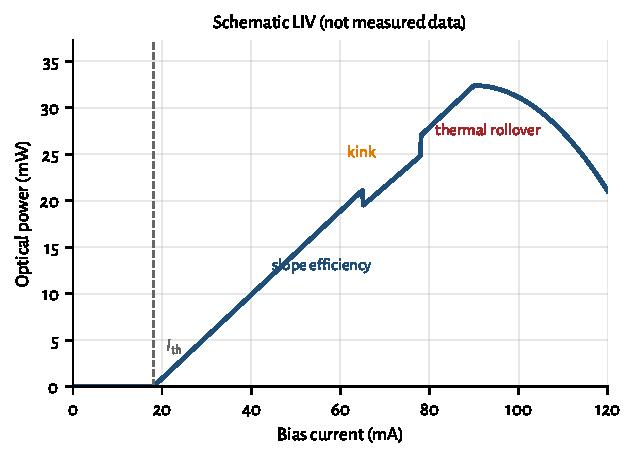
\includegraphics[width=0.85\linewidth]{figures/fig_liv_sketch.pdf}
\caption{Schematic LIV curve with threshold, slope, kink, and thermal rollover
labeled. Idealized for teaching; use measured LIV for pass/fail.
\label{fig:liv-sketch}}
\end{figure}

\paragraph{SMSR (side-mode suppression ratio).}
\firstterm{SMSR} SMSR is the power difference (dB) between the lasing mode and the
strongest side mode on an optical spectrum analyzer (OSA). Datacom single-mode
parts require high SMSR so side modes do not steal power or seed modal noise.
Spec-sheet floors are part-specific; treat the datasheet or ATP limit as
authoritative. SMSR collapse under temperature or aging is a reject: the laser is
leaving single-mode operation.

\paragraph{RIN (relative intensity noise).}
Measure RIN with a calibrated photodetector and RF spectrum analyzer (or a
dedicated RIN analyzer), under a controlled optical return loss. Distinguish
\emph{intrinsic} RIN (quiet bench, high ORL) from stressed
$\mathrm{RIN}_x\mathrm{OMA}$ used in Ethernet/MSA specs. IEEE 802.3 / 100G Lambda
class links cap $\mathrm{RIN}_{17.1}\mathrm{OMA}$ at $-136$~dB/Hz with 17.1~dB
ORL~\firstcite{rinspec}. Quiet datacom DFB/EML parts typically sit well below that
when feedback is controlled; CPO ELS designs care as much about feedback tolerance
as about the quiet number (\Cref{sec:rin-values,sec:rin}).

\begin{table*}[ht]
\refstepcounter{table}\label{tab:laser-meas}%
\centering
\setlength{\tabcolsep}{4pt}%
\footnotesize
\renewcommand{\arraystretch}{1.25}%
\begin{tabular}{@{}p{0.12\linewidth}p{0.18\linewidth}p{0.28\linewidth}p{0.36\linewidth}@{}}
\toprule
Parameter & Instrument & Pass/fail intent & Failure signature \\
\midrule
LIV & SMU + power meter / integrating sphere & $I_\mathrm{th}$, slope, kink-free bias window & high-temp rollover; kink in bias range \\
\addlinespace[1.5em]
SMSR & OSA & single-mode purity vs.\ datasheet/ATP & side modes rise with $T$ or age \\
\addlinespace[1.5em]
RIN & PD + ESA / RIN analyzer & intrinsic and stressed $\mathrm{RIN}_x\mathrm{OMA}$ & RIN rises with ORL; BER floor (\Cref{sec:rin}) \\
\addlinespace[1.5em]
Bias-driver noise & SMU vs.\ product bias board & $\mathrm{RIN}_{\mathrm{eq}}$ from $i_n$ (\Cref{sec:laser-drivers}) & RIN rises with rails on, flat vs.\ ORL \\
\addlinespace[1.5em]
Wavelength & OSA / wavemeter & grid placement, $d\lambda/dT$, $d\lambda/dI$ & walk off ring or MSA grid \\
\addlinespace[1.5em]
EAM bias (EML) & bias sweep + DCA/TDECQ & extinction, chirp, RLM & aging shifts absorption curve \\
\bottomrule
\end{tabular}
\par\medskip
{\raggedright\footnotesize\textbf{Table~\thetable.} Laser measurement playbook: what to
measure, with what, and what failure looks like.\par}
\end{table*}

Measure in order: LIV $\to$ SMSR $\to$ wavelength $\to$ RIN (quiet then
stressed ORL) $\to$ EAM or bias-driver checks as the path requires. Stop when
distributions across temperature and units support the bias window, grid, and
RIN policy in \Cref{tab:laser-prd} (see also
\Cref{tab:laser-engineering-checklist}). Do not keep measuring for its own
sake once those exits close.

\section{Laser drivers and the RIN budget}
\label{sec:laser-drivers}

Modulator RF drivers (\Cref{sec:drivers}) deliver swing and bandwidth into an EAM
or MZM. Laser \emph{bias} drivers are a different circuit: they set a quiet
constant current into the diode. Current noise on that path becomes optical
intensity noise and adds in the RIN budget of \Cref{sec:rin}. Confusing the two
is a common debug miss: a great SiGe PAM4 driver can still ruin a CW laser if its
supply or ground couples into the bias rail.

\paragraph{From current noise to equivalent RIN.}
Above threshold, optical power tracks bias approximately as
$P\propto(I-I_\mathrm{th})$. Relative intensity fluctuations then track relative
current fluctuations:
\[
\mathrm{RIN}_{\mathrm{eq,lin}}
\;\approx\;
\left(\frac{i_n}{I-I_\mathrm{th}}\right)^{\!2},
\qquad
\mathrm{RIN}_{\mathrm{eq}}[\mathrm{dB/Hz}]
\;=\;
20\log_{10}\!\left(\frac{i_n}{I-I_\mathrm{th}}\right),
\]
where $i_n$ is the one-sided current-noise density in A$/\sqrt{\mathrm{Hz}}$ at the
laser terminals (driver plus board pickup). The approximation assumes linear slope
efficiency and ignores intrinsic laser dynamics; it is a budget tool, not a device
model.

Worked numbers at $I-I_\mathrm{th}=50$~mA (typical CW DFB window): $i_n=500$~pA$/\sqrt{\mathrm{Hz}}$
maps to $\mathrm{RIN}_{\mathrm{eq}}\approx-160$~dB/Hz; $270$~pA$/\sqrt{\mathrm{Hz}}$
maps to about $-165$~dB/Hz. Commercial low-noise laser drivers quote roughly
$50$--$500$~pA$/\sqrt{\mathrm{Hz}}$ at 1~kHz depending on current range
(\Cref{tab:laser-driver-noise}); the Koheron DRV200 family is a concrete
example~\firstcite{koherondrv200}. Against a good datacom intrinsic RIN of
$-145$ to $-155$~dB/Hz (\Cref{sec:rin-values}), those 1~kHz densities look
comfortable. The budget tightens when $(I-I_\mathrm{th})$ is small (near
threshold, derated CW, or low-current VCSELs), when you integrate broadband
switching noise rather than a 1~kHz spot, or when SerDes/DSP rails dump discrete
tones onto the bias network.

\begin{table*}[ht]
\refstepcounter{table}\label{tab:laser-driver-noise}%
\centering
\setlength{\tabcolsep}{4pt}%
\footnotesize
\renewcommand{\arraystretch}{1.25}%
\begin{tabular}{@{}p{0.28\linewidth}p{0.18\linewidth}p{0.22\linewidth}p{0.26\linewidth}@{}}
\toprule
Driver class (example) & $i_n$ @ 1~kHz & $\mathrm{RIN}_{\mathrm{eq}}$ @ 50~mA & What it means \\
\midrule
Ultra-low-noise CW (DRV200-A-40) & 55~pA$/\sqrt{\mathrm{Hz}}$ & $\approx-179$~dB/Hz & Bench / metrology floor \\
\addlinespace[1.5em]
Low-noise CW (DRV200-A-200) & 270~pA$/\sqrt{\mathrm{Hz}}$ & $\approx-165$~dB/Hz & Typical quiet CW source \\
\addlinespace[1.5em]
Higher-current CW (DRV200-A-400) & 480~pA$/\sqrt{\mathrm{Hz}}$ & $\approx-160$~dB/Hz & Still below $-155$ intrinsic \\
\addlinespace[1.5em]
Shared digital LDO, poor PSRR & often $\gg$1~nA$/\sqrt{\mathrm{Hz}}$ + tones & can exceed $-145$ & False ``RIN'' on ESA \\
\bottomrule
\end{tabular}
\par\medskip
{\raggedright\footnotesize\textbf{Table~\thetable.} Bias-driver current noise converted to
equivalent RIN at $I-I_\mathrm{th}=50$~mA using
$\mathrm{RIN}_{\mathrm{eq}}=20\log_{10}(i_n/(I-I_\mathrm{th}))$. Densities for the
DRV200 rows are from the Koheron datasheet at 1~kHz; the last
row is qualitative (board-dependent).\par}
\end{table*}

\paragraph{CW / ELSFP / CW-WDM paths.}
For external CW sources feeding Si or TFLN modulators, design the bias path as a
low-noise current source with high supply rejection, local decoupling at the diode,
and a star ground that does not share return with SerDes switching currents.
Automatic power control (\firstterm{APC}) loops that close through a monitor PD
suppress slow drift; keep the loop bandwidth well below the RIN measurement band
and quiet enough that the loop itself does not inject intensity noise. ELSFP and
CW-WDM modules hide this circuitry inside the pluggable
(\Cref{sec:elsfp,sec:cwwdm-laser}); acceptance still needs module-level RIN with
the host bias and management rails connected, not only a quiet SMU on the bare die.

\paragraph{DML and EML.}
A \term{DML} shares one diode for bias and RF: a bias tee (or on-chip bias network)
combines a quiet DC source with the RF driver. Excess RF driver broadband noise,
poor tee isolation, or supply ripple on the bias arm all raise measured RIN and
chirp-related penalties. An \term{EML} splits the problem: keep the DFB bias as
quiet as a CW source, and treat the EAM RF driver under \Cref{sec:drivers}. EAM
drive amplitude sets extinction and chirp; DFB bias noise still lands in optical
intensity before the modulator.

\paragraph{What to measure on the bench.}
Bisect electrical vs.\ optical RIN:
\begin{enumerate}
\item Measure intrinsic RIN with a quiet SMU or known low-noise driver and high ORL
      (\Cref{sec:laser-params}).
\item Repeat with the product bias board / module rails connected. Any rise is
      driver or supply contribution, not laser physics.
\item Sweep ORL. Rise with reflection is feedback-driven laser RIN
      (\Cref{sec:rin-values}); rise independent of ORL points at the electrical path.
\item Look for discrete spurs on the ESA (switching frequencies, CMIS clocks). Spurs
      fail stressed $\mathrm{RIN}_x\mathrm{OMA}$ even when the broadband floor looks
      fine (\Cref{sec:rin-values}).
\end{enumerate}

\keyidea{Treat laser bias noise as a RIN term:
$\mathrm{RIN}_{\mathrm{eq}}\approx(i_n/(I-I_\mathrm{th}))^2$. Quiet CW drivers at
tens to hundreds of pA$/\sqrt{\mathrm{Hz}}$ usually sit under a $-145$~dB/Hz
intrinsic floor at 50~mA; digital supply pickup, near-threshold bias, and DML bias-tee
leakage are what actually burn the budget.}

\section{How lasers fail}
\label{sec:how-lasers-fail}

Six mechanisms account for most laser field returns. Each has a distinct
telemetry signature, so classify before you open FA.

\begin{description}
\item[Threshold current increase] $I_\mathrm{th}$ rises from its ship value at
      fixed temperature, usually with slope efficiency dropping in step. Points to
      active-region or facet degradation (\Cref{sec:laser-aging}).
\item[Slope efficiency degradation] Output power per unit bias current falls even
      when $I_\mathrm{th}$ is stable. A separate wear-out track from threshold rise;
      both show up on the same LIV sweep.
\item[Wavelength drift] The lasing line walks off its grid slot or ring resonance.
      Distinguish laser drift from TEC or ring drift by holding one actuator fixed
      and moving the other (\Cref{sec:locking-techniques,ch:wdm}).
\item[Aging (SMSR collapse, mode hopping)] Side modes grow relative to the main
      mode, or the laser hops between modes under temperature or current. An OSA
      trend over time is the tell.
\item[Thermal runaway] A positive feedback loop where higher junction temperature
      raises threshold current and cuts slope efficiency, so more drive power turns
      to heat for the same optical output, raising temperature further until the
      TEC saturates and the laser rolls over. Triggered by a failed or saturated
      TEC, a blocked heat path, or operation above the rated thermal class. Distinct
      from ordinary wear-out because it is fast (minutes, not months) once it
      starts; the failure-analysis handbook has the full symptom-to-cause
      breakdown (\Cref{sec:fm-thermal-runaway}).
\item[Monitor photodiode failure] The control loop's own sensor drifts or fails,
      so the laser looks unstable when the real fault is in the feedback path, not
      the gain medium (\Cref{sec:lasers-how-fails}).
\end{description}

\section{Separate thermal behavior from long-term aging}
\label{sec:laser-thermal-vs-aging}

Thermal response is reversible on the time scale of a temperature sweep or
cycle. It changes threshold current, slope efficiency, wavelength, EAM bias,
TEC current, and ring alignment. Measure it with controlled case-temperature
sweeps, loaded thermal corners, heater sweeps, and thermal cycling. Repeat the
measurement after returning to the starting temperature. Recovery points toward
an operating-point or control problem.

Long-term aging is cumulative. Threshold current rises, slope efficiency falls,
contacts degrade, defects grow, and an absorption or spectral curve can move
permanently. Measure those changes with HTOL, accelerated life testing, and
periodic LIV, spectrum, and modulation readouts. A temperature cycle can expose a
weak attach or calibration error, but it does not by itself establish a lifetime
acceleration model.

Do not merge the data sets. A high-temperature BER failure that clears at room
temperature needs thermal-margin work. A room-temperature baseline that keeps
moving after each stress interval needs an aging or damage hypothesis.

\section{Calibration: what drifts and what triggers retuning}
\label{sec:laser-calibration}

Calibration exists because no transmitter runs at a datasheet point. Every unit
has its own threshold, slope, absorption curve, quadrature point, and resonance,
and each of those moves with temperature and age. The operating points a product
actually stores are:

\begin{description}
\item[Laser bias / APC target] the bias current or monitor-PD power setpoint
      that holds launch power. Drifts as threshold rises and slope falls with
      age (\Cref{sec:laser-aging}); a drifting monitor PD corrupts it silently
      (\Cref{sec:lasers-how-fails}).
\item[EAM bias (EML)] the reverse-bias point that sets extinction and chirp.
      Moves with case temperature and with absorption-curve aging, so production
      parts store bias versus temperature, not one number.
\item[MZM quadrature] the phase bias that holds the modulator at its linear
      point. Drifts with temperature, stress, and age; a bias-control loop tracks
      it, and a railed loop is a telemetry alarm, not a retune request.
\item[Ring heater / lock point] the tuner power that aligns resonance to the
      laser line. Consumes headroom as ambient rises and neighbors heat; a railed
      DAC means the tuning range is exhausted
      (\Cref{sec:locking-techniques,sec:thermal-xtalk}).
\end{description}

Tables are usually segmented by temperature. Segment boundaries are a real
failure mode: the debug story in \Cref{sec:lasers-how-debugged} is a healthy
laser reading the wrong temperature segment after thermal cycling. Keep
calibration tables under change control and record the table version with every
test result, or failures cannot be replayed.

Recalibration should be triggered by evidence, not habit: a control-loop error
residual that no longer converges, an actuator (TEC, heater, bias DAC) that
approaches its rail, telemetry that disagrees with an external reference, a
temperature excursion beyond the table range, or a repair, rework, or firmware
change that invalidates stored coefficients. ATP must verify calibration at the
temperature corners the fleet will see, not only at the station ambient
(\Cref{sec:prod-corners}).

\section{How lasers are qualified}
\label{sec:how-lasers-qualified}

Qualification projects the failure mechanisms of \Cref{sec:how-lasers-fail}
forward from a short bench test to years of field life. Three stress classes do
the work:

\begin{description}
\item[HTOL (high-temperature operating life)] Run a sample lot at elevated
      temperature and bias for a fixed duration (often 1000 hours) and track LIV,
      SMSR, and wavelength drift. HTOL is the primary input to the Arrhenius life
      projection below.
\item[Burn-in] A shorter, sometimes 100\%-screen stress that removes
      infant-mortality units before ship, rather than projecting life. Burn-in
      trades test time for escape rate (\Cref{sec:hvm-test}).
\item[Environmental stress] Temperature cycling, damp heat, vibration, and shock
      catch packaging, attach, and mechanical failure modes that HTOL does not.
      They qualify different risks and should not be treated as substitutes for
      long-term aging data (\Cref{sec:gr468}).
\end{description}

Together with the Arrhenius acceleration factor, these three stresses turn a
qualification lot into a defensible FIT number.

\paragraph{Observable aging signatures.}
Watch LIV and spectrum over HTOL or field life:
\begin{itemize}
\item threshold rise and slope drop (active-region / facet degradation);
\item SMSR collapse (mode competition);
\item EAM bias creep on EMLs (absorption curve shift $\to$ TDECQ/RLM drift);
\item RIN rise under feedback (ORL or isolator failure);
\item COD\firstterm{COD} (catastrophic optical damage) at the facet under overstress.
\end{itemize}
Each signature should appear in the ATP and in field telemetry triage
(\Cref{sec:fleet-triage,sec:gr468}).

\section{Aging curves, derating, and fleet FIT}
\label{sec:laser-aging}

Lasers wear out. At fleet scale that is not a footnote; it sets architecture
(ELSFP vs.\ integrated laser) and operating policy (derating, burn-in).

\paragraph{Arrhenius life projection.}
\firstterm{Arrhenius} Telcordia GR-468-CORE qualifies optoelectronic parts with
accelerated stress (HTOL\firstterm{HTOL}, temperature cycle, damp heat) and projects field life
with Arrhenius acceleration~\firstcite{gr468}:
\[
\mathrm{AF}
= \exp\!\left[\frac{E_a}{k_B}\left(\frac{1}{T_\mathrm{use}}-\frac{1}{T_\mathrm{stress}}\right)\right],
\]
where $E_a$ is the activation energy for the wear-out mechanism under test, $k_B$
is Boltzmann's constant, and temperatures are absolute. Document $E_a$, sample
size, and confidence bounds when converting a 1000-hour HTOL lot into field-year
FIT. Activation energies are mechanism-specific; use the value justified in the
qual plan, not a generic number copied from another product.

\begin{figure*}[ht]
\centering
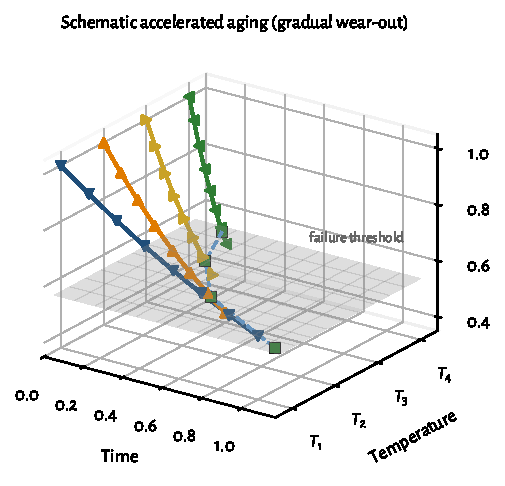
\includegraphics[width=0.92\linewidth]{figures/fig_accelerated_aging.pdf}
\caption{Schematic accelerated aging for gradual laser wear-out. A degradation
parameter (for example optical power at fixed bias, or threshold current rise
mapped to a falling health metric) is tracked versus time at several stress
temperatures $T_1 < T_2 < T_3 < T_4$. Higher temperature reaches the failure
threshold sooner. The dashed curve on the threshold plane is the
time-to-failure trend that Arrhenius acceleration turns into a use-condition
life estimate. Not measured data. Valid only for one thermally activated
mechanism with junction temperature as the stress variable; sudden modes such
as COD or ESD do not draw this surface.
\label{fig:accelerated-aging}}
\end{figure*}

\Cref{fig:accelerated-aging} is the mental model behind HTOL: same starting
health, faster drift at higher temperature, a defined end-of-life threshold, and
shorter time-to-failure as stress rises. For lasers the vertical axis is usually
tied to LIV or power at constant current; the temperature axis must be junction
temperature, not only chamber set point.

\paragraph{When the projection is valid.}
Acceleration assumes the stress speeds up the \emph{same} physical mechanism the
fleet will see. The projection fails in two ways: the stress activates a
mechanism the field never sees (solder creep or moisture ingress at a stress
temperature the product never reaches), or the field sees a mechanism the stress
never exercises (connector wear, bias-rail transients, thermal cycling from
traffic load). So a qual number is a hypothesis, not a fact: compare field-return
Pareto and failure signatures against the qual projection, and treat divergence
as evidence that $E_a$ or the mechanism model is wrong, not that the fleet is
unlucky (\Cref{sec:fleet-triage}). Sudden fails (COD, ESD, cracked fiber attach)
sit outside \Cref{fig:accelerated-aging}; classify those separately before you
fit Arrhenius parameters.

\paragraph{Derating.}
Run below absolute-max current, case temperature, and optical power. Derating
extends wear-out life and reduces COD risk. Uncooled datacom parts already sit near
thermal limits at high case temperature; cooled or faceplate ELSFP modules
(\Cref{sec:elsfp}) buy headroom by moving heat off the ASIC package.

\paragraph{Worked FIT example (assumptions labeled).}
\label{sec:fit-example}
FIT is failures per $10^9$ device-hours. For illustration only, assume 50~FIT per
laser (confirm against your supplier qual; do not treat 50 as a measured claim)
and a fabric with $5\times10^5$ lasers (order-of-magnitude for a large AI cluster
with several optical links per accelerator). Expected failures per day:
\[
\frac{5\times10^5 \times 50 \times 24}{10^9}
\approx 0.6\ \text{laser failures/day}.
\]
That is why field-replaceable ELSFP modules, burn-in screens, and derating are
design inputs, not afterthoughts (\Cref{ch:reliability}).

\section{ELS and ELSFP: architecture, pinout, qual}
\label{sec:elsfp}

\term{ELSFP}\firstterm{ELSFP} (External Laser Small Form-Factor Pluggable) is the
OIF form factor for faceplate-pluggable CW laser modules that feed co-packaged
optical engines~\firstcite{elsfp}. The lasers sit at the coolest part of the
system (front panel), hot-swap when they fail, and keep thermal load off the ASIC
and photonic engine.

\paragraph{Mechanical and optical.}
The module uses a card-edge electrical interface and a blind-mate multi-fiber
optical connector at the rear (MT-class ferrules), which improves eye safety for
high CW power by keeping live fiber inside the chassis~\firstcite{elsfp}. One ELSFP
can feed more than one optical engine. OIF defines optical power classes, thermal
classes, and wavelength assignments (e.g.\ DR-type 1311~nm and FR-type CWDM4
grids) so hosts and modules interoperate.

\paragraph{Management and hot-swap.}
ELSFP uses CMIS and the CMIS module state machine over TWI. On plug-in the module
resets, initializes management, and stays in low-power mode with lasers
\emph{off} until the host transitions it to ModuleReady and explicitly enables
lasers~\firstcite{elsfp}. \texttt{ModPrsL} and \texttt{IntL} support presence detect
and asynchronous alarms for safe hot-swap.

\paragraph{Electrical pinout (OIF-ELSFP-02.0 Table~7).}
Twenty-four contacts: multiple 3.3~V VCC and GND pins, module reset (\texttt{ResetL}),
low-power mode (\texttt{LPModeL}), two-wire serial management (\texttt{SCL}/\texttt{SDA}),
presence (\texttt{ModPrsL}), and interrupt (\texttt{IntL}), plus reserved pins for
future power/ground~\firstcite{elsfp}. \Cref{tab:elsfp-pins} summarizes the published
map.

\begin{table*}[ht]
\refstepcounter{table}\label{tab:elsfp-pins}%
\centering
\setlength{\tabcolsep}{4pt}%
\footnotesize
\renewcommand{\arraystretch}{1.25}%
\begin{tabular}{@{}p{0.08\linewidth}p{0.16\linewidth}p{0.28\linewidth}p{0.42\linewidth}@{}}
\toprule
Pin & Function & Requirements & Notes \\
\midrule
1--3 & VCC & 1.5~A, 3.3~V & with noise filtering \\
\addlinespace[1.5em]
4 & TBD & reserved & future power \\
\addlinespace[1.5em]
5 & ResetL & pull-up 10~k$\Omega$ & reset module, LVTTL \\
\addlinespace[1.5em]
6 & LPModeL & MMC on only & low-power mode (low), LVTTL \\
\addlinespace[1.5em]
7 & TBD & reserved & future ground \\
\addlinespace[1.5em]
8--10 & GND & 1.5~A, 3.3~V & with noise filtering \\
\addlinespace[1.5em]
11 & TBD & reserved & --- \\
\addlinespace[1.5em]
12 & SCL & TWI clock & host 4.7~k$\Omega$ pull-up; module $\ge$10~k$\Omega$ \\
\addlinespace[1.5em]
13 & SDA & TWI data & same pull-ups as SCL \\
\addlinespace[1.5em]
14 & TBD & reserved & --- \\
\addlinespace[1.5em]
15--17 & GND & 1.5~A, 3.3~V & with noise filtering \\
\addlinespace[1.5em]
18 & TBD & reserved & future ground \\
\addlinespace[1.5em]
19 & ModPrsL & shorted to GND in module & presence (low), LVTTL \\
\addlinespace[1.5em]
20 & IntL & pull-up 10~k$\Omega$ & interrupt, LVTTL \\
\addlinespace[1.5em]
21 & TBD & reserved & future power \\
\addlinespace[1.5em]
22--24 & VCC & 1.5~A, 3.3~V & with noise filtering \\
\bottomrule
\end{tabular}
\par\medskip
{\raggedright\footnotesize\textbf{Table~\thetable.} ELSFP electrical pinout
(adapted from OIF-ELSFP-02.0 Table~7). Lasers power only in ModuleReady after host
command; default on plug-in is lasers off~\firstcite{elsfp}.\par}
\end{table*}

\paragraph{Qual hooks for suppliers.}
Acceptance test plans should cover the checklist in \Cref{tab:atp-laser,sec:supplier-exec}:
laser LIV/SMSR/RIN inside the module; optical power-class compliance; connector
mating cycles and contamination/ORL; burn-in before ship; CMIS register sanity;
and thermal class at rated case temperature. Module bring-up must also prove the
CMIS enable sequence and ModuleReady laser policy (\Cref{sec:bringup}). Field
returns split between laser wear-out and connector/fiber-attach faults; keep both
in the triage tree (\Cref{sec:fleet-triage}).

\section{Optical safety and laser classes}
\label{sec:laser-safety}

\subsection{Hazard and laser classes}

Laser safety for interconnects is governed by IEC 60825-1 (laser product
classification) and IEC 60825-2 (optical-fiber communication systems,
OFCS)~\cite{iec60825}. Classes run from Class 1 (safe under normal use) through
Class 1M (safe unless the beam is collected by optics), Class 3R/3B, and Class 4.
At 1310~nm and 1550~nm the beam is invisible, which raises the operational risk:
technicians cannot see exposure. The retinal-hazard band ends near 1400~nm, but
corneal and skin hazards remain, and single-mode power confined to a $\sim$9~\textmu m
core is high radiance even at modest milliwatt levels.

Short-reach datacom modules are usually engineered so each fiber port stays Class 1
or Class 1M under rated launch power. That is a design constraint on EML/DFB bias
and on how much power each lane launches, not a label you add after the fact.

\subsection{Hazard level = aggregate, not per-lane}

The safety case scales with \emph{total} launched power at an accessible location,
not with a single DFB data sheet. CW-WDM and ELS banks concentrate many lines on one
MT or MPO ferrule (\Cref{sec:elsfp}). A connector that breaks out eight or sixteen
fibers can exceed a per-lane Class 1 budget even when each lane is modest. IEC
60825-2 assigns hazard levels (1 through 4) to each accessible port in the OFCS
based on the radiant power that could escape during service~\cite{iec60825}. That
is why ELS architecture and fiber count drive classification, not the laser chip
alone.

\subsection{Open-fiber protection: APR and ALS}

When fiber continuity is lost, open connectors and broken fiber can expose
hazardous power. \term{APR}\firstterm{APR} (automatic power reduction) holds
output at or below Hazard Level 1M and probes for re-mate with safe low-power
pulses. \term{ALS}\firstterm{ALS} (automatic laser shutdown) cuts power entirely
and was common on older SDH links; for modern high-power systems APR with
automatic restart is the preferred pattern because restart probes stay within the
hazard limit~\cite{g664}. ITU-T G.664 requires power reduction to Hazard Level 1M
within about 3~s of a continuity break, a restart inhibit window, and restart only
at safe power.

These mechanisms tie directly to CMIS and bring-up policy: lasers enable only when
the host commands ModuleReady (\Cref{sec:bringup,sec:cmis}). APR/ALS is what makes
a live ELSFP hot-swap survivable in a running rack (\Cref{sec:prod-corners}).

\subsection{What validation and ops owe}

Optical safety is a validation deliverable, not a compliance sticker. ATP should
verify APR/ALS trip threshold and timing on representative open-fiber faults; label
modules and cages with the rated class; document max launched power per port and per
MPO breakout; and write service procedures for multi-fiber connectors. At fleet
scale, a hot-swap runbook that assumes ALS works but was never tested in ATP is a
real hazard. Fold the APR/ALS check into the ELS hot-swap corner in
\Cref{sec:prod-corners} alongside mate-cycle and ORL tests.

\section{CW-WDM source validation}
\label{sec:cwwdm-laser}

Multi-wavelength CW sources (CW-WDM MSA) feed dense ring or filter banks on a PIC
(\Cref{sec:cwwdm,ch:wdm}). Validation is per-channel plus cross-channel:

\begin{itemize}
\item power flatness across $\lambda$ (uneven OMA after the modulator bank);
\item per-channel SMSR and wavelength grid placement;
\item channel crosstalk and residual ASE between lines;
\item lock to microring resonances under temperature and neighbor heating
      (\Cref{sec:locking-techniques,sec:thermal-xtalk,sec:siring});
\item RIN and ORL sensitivity for each line (\Cref{sec:laser-params,sec:rin-values}).
\end{itemize}

Examples: Ayar Labs SuperNova (CW-WDM MSA-compliant, feeds TeraPHY)
~\firstcite{ayar,cwwdm}; Broadcom ELSFP banks on Tomahawk CPO
(\Cref{sec:cpo-status,sec:elsfp}); quantum-dot comb lasers (Ranovus, Quintessent)
aimed at many $\lambda$ from one chip. Source tests live here; locking and on-chip
MUX live in \Cref{ch:wdm}.

\section{Light-source supply strategy}
\label{sec:laser-suppliers}

The sourcing decision follows the same architecture fork as the optical design:
buy a merchant source, buy a serviceable external module, or bind the source to
the photonic package. Evaluate each path by qualification ownership, second-source
portability, lot traceability, test access, field replacement, and change-control
rights. A vendor list ages quickly and does not answer those questions.

\begin{description}
\item[Merchant DFB, EML, or CW die] preserve module-level design freedom and can
      support a second source, but the integrator owns attach, driver match,
      screening, and package reliability.
\item[External CW-WDM or ELSFP module] moves source qualification and management
      into a replaceable unit. The system still owns connector, ORL, hot-swap,
      and host interoperability (\Cref{sec:elsfp,sec:cwwdm-laser}).
\item[Multi-wavelength source] reduces source count and can simplify WDM fan-out,
      but couples channel yield, power flatness, control, and replacement into one
      unit (\Cref{sec:cwwdm-laser}).
\item[Source integrated with the PIC] reduces optical interfaces and can improve
      density, but makes laser yield and wear-out part of package yield and
      service life.
\end{description}

\begin{table*}[ht]
\refstepcounter{table}\label{tab:laser-suppliers}%
\centering
\setlength{\tabcolsep}{5pt}%
\renewcommand{\arraystretch}{1.25}%
\begin{tabular}{@{}p{0.28\linewidth}p{0.68\linewidth}@{}}
\toprule
Approach & Qualification ownership and risk \\
\midrule
Merchant DFB/EML/CW die & Integrator owns attach, driver match, screen, and module qual \\
\addlinespace[1.5em]
External CW-WDM / ELSFP module & Supplier owns source module; system owns interface and service qual \\
\addlinespace[1.5em]
Multi-wavelength source & Shared yield, power-flatness, and replacement risk across channels \\
\addlinespace[1.5em]
Source integrated with PIC & Highest density; laser yield and life become package risks \\
\bottomrule
\end{tabular}
\par\medskip
{\raggedright\footnotesize\textbf{Table~\thetable.} Light-source sourcing paths
and the qualification ownership each one creates.\par}
\end{table*}
\FloatBarrier

\subsection{Reading the supplier ownership matrix}
\label{sec:laser-suppliers-read}

\Cref{tab:laser-suppliers} is a qualification-ownership map. The fork decides
who owns life data, screens, and field service, not only who ships a die.

\paragraph{Merchant DFB / EML / CW die.}

\textbf{Purpose.}
Who owns attach, driver match, module screen, and package reliability when
the source is a merchant die?

\textbf{Uncertainty removed.}
Die datasheets do not qualify the module. After ownership is explicit, the
integrator knows which FAIR, ATP, and HTOL packages stay in-house.

\textbf{Evidence the other party still owes.}
Die-level LIV, SMSR, RIN, and life sample data from the merchant; change
control on epi and process.

\textbf{Decision unlocked.}
Accept integrator-owned module qual, or reject the path if attach and screen
capability are missing.

\textbf{Risk if ownership is assumed wrong.}
You treat a die cert as module qual and discover attach or driver match in
the fleet.

\paragraph{External CW-WDM / ELSFP module.}

\textbf{Purpose.}
What does the source supplier own versus what the system still must qualify?

\textbf{Uncertainty removed.}
A replaceable ELS moves source life into a field unit, but connector, ORL,
hot-swap, and host interop remain system-owned (\Cref{sec:elsfp}).

\textbf{Evidence the other party still owes.}
Supplier: source-module ATP, CMIS, life, and mate ratings. System: optical
mate, ORL plant, service sequence, and engine bring-up with light present.

\textbf{Decision unlocked.}
Approve ELS architecture only when both ownership packs exist.

\textbf{Risk if ownership is assumed wrong.}
You qualify the laser module and skip the optical interface that fails first
in service.

\paragraph{Multi-wavelength source.}

\textbf{Purpose.}
How do channel yield, power flatness, and replacement couple across the
comb?

\textbf{Uncertainty removed.}
One weak channel can scrap or derate the whole source. Shared control means
shared field risk (\Cref{sec:cwwdm-laser}).

\textbf{Evidence required.}
Per-channel power and wavelength distributions, flatness over temperature,
and a replacement/service policy when one channel fails.

\textbf{Decision unlocked.}
Accept coupled yield, require channel redundancy, or split into multiple
sources.

\textbf{Risk if ownership is assumed wrong.}
You buy ``one laser'' economics and inherit N-channel fail modes without
N-channel screens.

\paragraph{Source integrated with PIC.}

\textbf{Purpose.}
When laser yield and wear-out become package risks, who owns life and
service?

\textbf{Uncertainty removed.}
Density gains remove a replaceable optical interface. Failures then pull the
engine or package, not a pluggable source.

\textbf{Evidence required.}
Package-level life, known-good attach, and a service model that matches
non-replaceable sources.

\textbf{Decision unlocked.}
Accept integrated risk for density, or keep ELS/merchant die for field
replaceability.

\textbf{Risk if ownership is assumed wrong.}
You qualify the die physics and underfund package yield and fleet
replacement cost.

\subsection{Why ownership order matters}

Choose the service and ownership model before you freeze the optical
architecture. An external source is replaceable and adds a managed interface.
An integrated source removes that interface and places source yield inside
the package. Qualify the architecture you will service, not only the laser
die.

\subsection{Learning summary}

\begin{description}
\item[Merchant die] Integrator owns module qual; merchant owns die life data.
\item[ELS / CW-WDM module] Supplier owns source; system owns mate, ORL, swap.
\item[Multi-wavelength] Channels share yield and replacement risk.
\item[Integrated PIC] Laser life is package life; plan service accordingly.
\end{description}

\aside{The fork is a reliability and ownership decision. An external source makes
the source replaceable but adds a managed optical interface. An integrated source
removes that interface but places source yield and wear-out inside the package.
Qualify the architecture you will service, not only the laser die.}

\section{Why lasers are the reliability bottleneck}

At the scale of a large optical fleet the laser is usually the
reliability-limiting component. It is an active device with wear-out physics that
passive optics and even photodiodes largely lack:

\begin{itemize}
\item \term{Catastrophic optical damage} (COD) at the facet.
\item Gradual facet and active-region degradation (accelerated by temperature,
      following Arrhenius kinetics; \Cref{sec:laser-aging}).
\item EAM aging in EMLs; coupling and solder drift in packaged assemblies.
\end{itemize}

Because failures scale with the number of lasers, a fleet of $100{,}000$+ links
turns a modest per-laser FIT rate into a steady stream of field failures
(\Cref{sec:fit-example,sec:gr468}). The mitigations shape architecture:
field-replaceable external laser sources (ELSFP, CW-WDM),
redundancy, burn-in screening to weed out infant mortality, and derating (running
lasers below their maximum to extend life).

\section{Margin erosion over temperature, lot, and life}
\label{sec:laser-margin-erosion}

A link rarely loses all margin in one event. The source can lose launch power as
slope efficiency falls. Connector loss and ORL can rise after service. EAM or
MZM bias can move. A ring can consume spectral headroom as its heater approaches
range. Driver noise can raise the BER floor while none of these changes violates
its stand-alone limit.

Track five ledgers:
\begin{description}
\item[Power margin] launch power, coupling, connector and MUX loss, receiver
      sensitivity, and aging reserve.
\item[Noise margin] intrinsic and feedback-driven RIN, bias-rail noise, receiver
      noise, and crosstalk.
\item[Timing margin] source and modulator bandwidth, dispersion, driver and host
      jitter, and equalization reserve.
\item[Spectral margin] laser wavelength, SMSR, filter or ring passband, thermal
      drift, and lock range.
\item[Control margin] headroom in APC, TEC, heaters, ring lock, bias DACs, and
      calibration tables. A railed loop can fail the link while the diode is
      still healthy.
\end{description}

Recompute the link at combined production corners. A nominal part at nominal
temperature says little about whether a slow loss in two ledgers will push a
tail unit across the pre-FEC BER limit. \Cref{sec:prod-corners,tab:fleet-triage}
carry the same ledgers into validation and fleet triage. The interview review
compresses this checklist in \Cref{sec:interview-margin-ledgers}. The wall-chart
form is \Cref{sec:tree-margin-budget}.

\begin{dectree}
Nominal system margin
  |
Temperature debit
  |
Voltage / power-quality debit
  |
Channel / connector debit
  |
Manufacturing variation
  |
Aging / wear
  |
Interoperability variation
  |
Remaining margin
  |
Above deployment requirement?
  |-- YES --> proceed
  |-- NO  --> redesign / restrict / recalibrate / reject
\end{dectree}

Not every debit is naturally in decibels. Depending on the subsystem, remaining
margin may be optical power, sensitivity, BER or FEC headroom, eye or TDECQ,
jitter, control range, lifetime, or yield. Validation often measures the net
externally visible result; do not double-count internal penalties the test
cannot separate (\Cref{sec:link-budget}).

\section{Engineering lens}
\label{sec:lasers-engineering-lens}

\subsection{How it works}

A laser is an active device with wear-out physics, which makes it both the first
line of the link budget and the fleet's reliability bottleneck. The chapter's
device families and LIV/SMSR/RIN measurements all serve one question: will this
source stay in spec for years at temperature?

\subsection{How it is measured}
\label{sec:lasers-how-measured}

Qualify the laser as a set of curves across temperature, bias, ORL, and age, not a
room-temperature data-sheet point. The measurement playbook (LIV, SMSR, RIN,
wavelength, and EAM checks with their instruments and pass/fail intent) is in
\Cref{sec:laser-params,tab:laser-meas}; the stress classes that project field life
are in \Cref{sec:how-lasers-qualified,sec:laser-aging,sec:gr468}~\cite{gr468}.

\subsection{How it fails}
\label{sec:lasers-how-fails}

The six field-return mechanisms are catalogued in \Cref{sec:how-lasers-fail}:
threshold rise, slope droop, wavelength drift, aging (SMSR collapse and mode
hopping), thermal runaway, and monitor-photodiode failure. Manufacturing adds die,
wafer, lot, and assembly spread to every one. The mechanism that most often
misleads triage is a healthy laser behind a bad feedback sensor, so it gets the
worked callout below.

\failuremode{Monitor photodiode drift}{Reported power falls or the bias loop moves,
but an external power meter does not show the same change.}{Monitor-PD responsivity
drift, transimpedance gain error, contamination in the monitor path, or a bad
calibration coefficient.}{External power meter, monitor current, bias current,
LIV, and loop error versus temperature.}{Repair the monitor path or calibration,
add disagreement alarms, and do not raise laser bias to compensate for a false
reading.}

\subsection{How it is debugged}
\label{sec:lasers-how-debugged}

For power degradation, compare external optical power, monitor current, bias, and
case temperature before changing the setpoint. Rerun LIV at the failing
temperature and compare it with ship data. If LIV moved, inspect SMSR, wavelength,
and RIN to classify active-region, facet, or modal change. If LIV is stable, move
to coupling, connector, monitor-PD, and control-loop checks. For a wavelength
excursion, inspect OSA data and TEC current together. For a bias anomaly, replace
the product driver with a quiet source before blaming the diode.

\debugstory{BER worsened after thermal cycling while average optical power stayed
in range.}{The DCA showed that extinction ratio had collapsed. LIV and SMSR were
unchanged, and an EAM bias sweep restored the eye.}{The light source was healthy,
but its modulator operating point was wrong.}{A calibration table used the wrong
temperature segment after the cycle.}{The table and screening limits were fixed,
and EAM bias sweep data became part of the thermal-cycle readout.}

\section{Engineering checklist}
\label{sec:lasers-checklist}

\begin{table*}[ht]
\refstepcounter{table}\label{tab:laser-engineering-checklist}%
\centering
\setlength{\tabcolsep}{4pt}%
\footnotesize
\renewcommand{\arraystretch}{1.25}%
\begin{tabular}{@{}p{0.20\linewidth}p{0.34\linewidth}p{0.40\linewidth}@{}}
\toprule
Decision or test & Question it answers & Evidence to retain \\
\midrule
Architecture & Does the source and modulation path close reach, rate, power, cost, and service? & Requirement allocation and rejected alternatives \\
\addlinespace[1.5em]
LIV & Is the operating window clear of threshold, kinks, and rollover? & Curves by unit, lot, temperature, and age \\
\addlinespace[1.5em]
Spectrum & Does wavelength and SMSR stay inside the assigned grid and filter passband? & OSA or wavemeter data across corners \\
\addlinespace[1.5em]
RIN and ORL & Does noise margin survive the reflection environment? & Quiet and stressed RIN with stated ORL and bandwidth \\
\addlinespace[1.5em]
Modulation & Does bias, drive, chirp, and bandwidth close the eye? & Bias sweeps, TDECQ or equivalent, and driver conditions \\
\addlinespace[1.5em]
Thermal behavior & Are reversible shifts within control and actuator range? & Temperature and heater sweeps, TEC current, recovery data \\
\addlinespace[1.5em]
Long-term aging & Which parameters drift permanently, and at what rate? & HTOL intervals, LIV, spectrum, and modulation trends \\
\addlinespace[1.5em]
Manufacturing & Can the ATP catch bad units and lot drift at useful test cost? & Limits, guard bands, GR\&R, yield, and reaction plan \\
\addlinespace[1.5em]
Fleet operation & Which monitors distinguish source, modulator, cooler, and optical path? & Telemetry map, alarm thresholds, and golden baselines \\
\bottomrule
\end{tabular}
\par\medskip
{\raggedright\footnotesize\textbf{Table~\thetable.} Source and modulation
engineering checklist. Each row ties a decision to evidence, not only a test
name.\par}
\end{table*}
\FloatBarrier

\subsection{Reading the laser engineering checklist}
\label{sec:lasers-checklist-read}

\Cref{tab:laser-engineering-checklist} is the decision sequence for a laser
program. Measurement methods for LIV, SMSR, RIN, and aging are taught earlier
in this chapter; the notes below focus on what each row unlocks and when you
may leave it.

\paragraph{Architecture.}

\textbf{Purpose.}
Does the source and modulation path close reach, rate, power, cost, and
service?

\textbf{Uncertainty removed.}
Component enthusiasm does not allocate requirements. After architecture you
have a chosen path, rejected alternatives, and owners for lock, attach, and
life (\Cref{tab:source-mod-matrix,tab:laser-suppliers}).

\textbf{Exit criteria.}
\textbf{Exit when} requirement allocation and rejected alternatives are
written and reviewed.

\textbf{Decision unlocked.}
Freeze the path into \Cref{tab:laser-prd}, or reopen the matrix.

\textbf{Risk if skipped.}
You validate a hero topology that cannot be serviced or powered in the rack.

\paragraph{LIV.}

\textbf{Purpose.}
Is the operating window clear of threshold, kinks, and rollover across unit,
lot, temperature, and age (\Cref{sec:laser-params})?

\textbf{Exit criteria.}
\textbf{Exit when} kink-free bias windows and distributions support the
bias policy.

\textbf{Decision unlocked.}
Set bias and derate, or reject lots / redesign the window.

\textbf{Risk if skipped.}
Soft BER and sudden dark fails appear without a ship baseline to compare.

\paragraph{Spectrum.}

\textbf{Purpose.}
Do wavelength and SMSR stay inside the assigned grid and filter passband?

\textbf{Exit criteria.}
\textbf{Exit when} OSA or wavemeter data across corners meet grid and SMSR
floors.

\textbf{Decision unlocked.}
Approve channel assignment, tighten temperature policy, or reject modal risk.

\textbf{Risk if skipped.}
WDM unlock and modal noise show up as ``random'' BER.

\paragraph{RIN and ORL.}

\textbf{Purpose.}
Does noise margin survive the reflection environment the plant will present
(\Cref{sec:rin-values})?

\textbf{Exit criteria.}
\textbf{Exit when} quiet and stressed RIN at stated ORL and bandwidth meet
the BER-floor budget.

\textbf{Decision unlocked.}
Approve isolator-free or isolator-required design; set plant cleaning rules.

\textbf{Risk if skipped.}
Lab RIN looks fine; field ORL raises the floor.

\paragraph{Modulation.}

\textbf{Purpose.}
Do bias, drive, chirp, and bandwidth close the eye at baud?

\textbf{Exit criteria.}
\textbf{Exit when} bias sweeps and TDECQ (or equivalent) at named driver
conditions meet Tx quality limits (\Cref{sec:tdecq}).

\textbf{Decision unlocked.}
Freeze EAM/MZM/ring bias policy, or reject the modulator class for this rate.

\textbf{Risk if skipped.}
Average power passes while the eye fails under temperature.

\paragraph{Thermal behavior.}

\textbf{Purpose.}
Are reversible shifts within control and actuator range?

\textbf{Exit criteria.}
\textbf{Exit when} temperature and heater sweeps, TEC current, and recovery
data show control headroom at loaded corners.

\textbf{Decision unlocked.}
Approve thermal envelope, add heaters/TEC margin, or derate case $T$.

\textbf{Risk if skipped.}
Lock and calibration faults are misread as permanent aging.

\paragraph{Long-term aging.}

\textbf{Purpose.}
Which parameters drift permanently, and at what rate
(\Cref{sec:laser-aging})?

\textbf{Exit criteria.}
\textbf{Exit when} HTOL intervals with LIV, spectrum, and modulation trends
support the life claim or force derate.

\textbf{Decision unlocked.}
Accept FIT/replacement plan, or hold ship for life risk.

\textbf{Risk if skipped.}
Useful-life planning uses hope instead of a mechanism.

\paragraph{Manufacturing.}

\textbf{Purpose.}
Can the ATP catch bad units and lot drift at useful test cost
(\Cref{tab:atp-laser})?

\textbf{Exit criteria.}
\textbf{Exit when} limits, guardbands, GR\&R, yield, and a reaction plan
exist for the ship screens.

\textbf{Decision unlocked.}
Open volume screens, or hold for process control.

\textbf{Risk if skipped.}
Qualified engineering lots diverge from production without a catch point.

\paragraph{Fleet operation.}

\textbf{Purpose.}
Which monitors distinguish source, modulator, cooler, and optical path
(\Cref{sec:fleet-triage})?

\textbf{Exit criteria.}
\textbf{Exit when} telemetry map, alarm thresholds, and golden baselines are
named and owned.

\textbf{Decision unlocked.}
Arm fleet triage; feed escapes back into ATP.

\textbf{Risk if skipped.}
Field tickets cannot separate laser wear from connector or TEC faults.

\subsection{Why the checklist order matters}

Architecture first, or you characterize the wrong path. LIV and spectrum
establish semiconductor and channel health before RIN and modulation argue
about floors and eyes. Thermal separates reversible control from permanent
drift before aging claims. Manufacturing and fleet close the loop so life and
screens stay honest after ship. Later rows must not compensate for a missing
architecture or ship baseline.

\subsection{Learning summary}

\begin{description}
\item[Architecture] Does the path close the product?
\item[LIV / spectrum / RIN] Is the source healthy in its plant?
\item[Modulation / thermal] Does the eye and control survive corners?
\item[Aging] What drifts permanently, and how fast?
\item[Manufacturing / fleet] Can you screen it and triage it at volume?
\end{description}

\section{Interview takeaway}
\label{sec:lasers-design-review}

\keyidea{Measure LIV, SMSR, wavelength, and RIN as distributions across
temperature, lot, and age. Tie each requirement to an ATP row, each life claim to
a physical mechanism, and each field alarm to a measurement that separates the
laser from its driver, monitor, cooler, and optical path.}

\paragraph{Three questions to test yourself.}
\begin{enumerate}
\item Why is the laser typically the reliability-limiting component in an optical
      link?
\item Optical power fell but the monitor photodiode reports no change. What do
      you check?
\item How would you qualify a second laser supplier without assuming the first
      supplier's failure distribution?
\end{enumerate}

\chapter{WDM and wavelength-locked lasers}
\label{ch:wdm}

\textit{Read first:} why WDM; capture versus hold; thermal crosstalk;
laser-versus-ring isolation; one-lane versus all-lane signatures.

\textit{Deep dive:} SOA noise figure and gain placement; polarization on the CW
path; comb-source device classes.

\textit{Reference:} WDM grid table, MUX defect map, CW-WDM MSA grid details.

Early datacenter optics mostly ran one wavelength per fiber. That worked while
port counts were modest. At AI scale, fiber count itself becomes a first-order
cost and cable-plant problem, so the industry packed more channels onto each
strand. The price of that packing is control: once channel spacing tightens, or
once the modulator is a wavelength-selective ring, someone must keep laser and
filter locked together. In the architectures covered here, an explicit
wavelength-lock requirement strongly suggests a tight wavelength grid, a
wavelength-selective modulator or filter, or both. It does not uniquely prove
WDM or microring modulation; a single-channel resonant path can also need
stabilization. Ring and MZM device physics stay in
\Cref{sec:siring,sec:simzm}; per-$\lambda$ laser evidence and aging stay in
\Cref{ch:lasers}. This chapter covers grids, lock loops, thermal crosstalk, MUX
budget, and CW-WDM architecture.

\tradeoff{Dense WDM vs lock complexity}{Fiber count, faceplate density, and
bandwidth per strand}{Heaters, TEC, lock firmware, thermal crosstalk, and unlock
controls}{When fiber plant or connector count is the binding constraint}{Pay for
locking only when multiplexing is worth the control burden.}

\section{Why multiplex wavelengths at all}
\label{sec:why-wdm}

At $100{,}000$+ accelerator scale, every extra fiber is another connector,
another patch, and another failure mode. \term{Wavelength-division multiplexing}
(WDM)\firstterm{WDM} puts many independent channels on a single fiber, each on its own
wavelength, so bandwidth per fiber rises without adding fiber. Each wavelength
can still be an ordinary IM/DD channel. WDM and IM/DD are orthogonal; you run
IM/DD \emph{per wavelength}.

Historically the industry climbed a ladder of spacing. Coarse CWDM4 used
$\approx$20~nm slots and uncooled lasers. LAN-WDM tightened that for 2~km-class
FR4. Dense grids and then CW-WDM O-band combs for CPO pushed spacing into the
100--800~GHz class and made active locking mandatory. Those spacings are
standardized grids, not vendor choices: the 20~nm CWDM slots follow the ITU-T
G.694.2 wavelength grid (18 channels, 1271--1611~nm), and the 50/100/200~GHz
datacom DWDM spacings follow the ITU-T G.694.1 frequency grid anchored at
193.1~THz~\firstcite{ituG694}. CWDM4 uses the four O-band lines of that CWDM
grid; the CW-WDM combs in \Cref{sec:cwwdm} define their own O-band grids for
dense integration. \Cref{tab:wdm-grids} is that ladder as you will meet it in
short-reach AI optics today.

\begin{table*}[ht]
\refstepcounter{table}\label{tab:wdm-grids}%
\centering
\setlength{\tabcolsep}{3.5pt}%
\footnotesize
\renewcommand{\arraystretch}{1.25}%
\begin{tabular}{@{}p{0.16\linewidth}p{0.14\linewidth}p{0.12\linewidth}p{0.18\linewidth}p{0.32\linewidth}@{}}
\toprule
Grid family & Spacing (class) & Channels / fiber & Cooling / lock & Typical short-reach use \\
\midrule
CWDM4 & $\approx$20~nm & 4 & Uncooled; loose control & FR-class pluggables; faceplate WDM \\
\addlinespace[1.5em]
LAN-WDM & $\approx$800~GHz ($\approx$4--5~nm @ 1310~nm) & 4 & Cooled or tight open-loop & 2~km-class FR4 (edge of book scope) \\
\addlinespace[1.5em]
Datacom DWDM & 200/100/50~GHz & many & Locked to grid & Discrete DFB/EML DWDM modules \\
\addlinespace[1.5em]
CW-WDM / CPO O-band & 100--800~GHz class (MSA spans) & 8 / 16 / 32 & Locked; often ring-tuned & CPO engines, optical I/O chiplets \\
\bottomrule
\end{tabular}
\par\medskip
{\raggedright\footnotesize\textbf{Table~\thetable.} WDM grids for short-reach AI interconnects.
CW-WDM MSA normative grids sit in O-band with 9/18/36~nm spans and 8/16/32-line
sets (\Cref{sec:cwwdm}); spacing is set by the chosen span and channel count, not
by Ethernet CWDM4.\par}
\end{table*}

\textbf{Exit when} fiber count, lock burden, and cooling class pick one grid
family for the product. \textbf{Decision unlocked:} accept uncooled CWDM4, or
fund locked denser grids (LAN-WDM, DWDM, CW-WDM) with the control page they
require.

\section{Why ``locked'' is the operative word}
\label{sec:why-locked}

WDM alone does not force active locking. CWDM4 packs four wavelengths with enough
spacing that uncooled lasers can wander and still stay in their slots. Active
locking becomes important when the channel spacing and filter guardband are
tight, or when the modulator itself is resonant. Those two situations drive most
modern CPO and dense optical-I/O control loops. Calculate total drift and
manufacturing variation against the usable passband before choosing calibration,
temperature control, or closed-loop locking.

\subsection{Tight DWDM grids}

To pack channels at 50--200~GHz class spacing\firstterm{DWDM}, each laser must sit on its grid
slot or adjacent channels collide. Emphasizing ``locking'' therefore hints at
spacing tighter than CWDM. You do not stress locking for coarse, uncooled CWDM4;
you do as soon as the grid looks like LAN-WDM, datacom DWDM, or a CW-WDM comb.

\subsection{Microring modulators and WDM locking}

Resonant ring and microdisk modulators are commonly used where density and
capacitance matter (\Cref{sec:siring}). Silicon microring resonance often shifts
by order-of-magnitude several to roughly ten gigahertz per degree Celsius,
depending on geometry, material stack, and operating point; prefer the measured
product coefficient when building a lock budget. Even a stable laser is then not
enough: the laser and the ring must stay aligned. Either lock the laser to the
ring, or thermally tune the ring onto the laser with a feedback loop. That
laser--ring co-locking is the central control problem in ring-based WDM links and
in co-packaged optics, and it is why neighbor heat and case-temperature ramps
belong in validation, not only in the thermal section of a datasheet.

A Mach--Zehnder is comparatively broadband, so it normally does not require the
same carrier-to-modulator resonance lock, although its laser must still remain
inside the WDM grid and MUX passband (\Cref{sec:simzm}).
\section{WDM filters, grids, and on-chip multiplexing}
\label{sec:wdm-hardware}

WDM is not only lasers and locking (\Cref{sec:cwwdm}): the PIC\firstterm{PIC} needs wavelength
selective routing. The MUX/demux stage is a first-class link-budget line item
(\Cref{sec:link-budget}), not a packaging footnote.

\paragraph{Signal journey through the MUX.}
Follow one wavelength from laser (or comb line) through the modulator, into the
MUX, across the plant, and out the demux to the receiver. Stage insertion loss
lowers OMA on every lane. Passband ripple and MUX imbalance make the weakest
$\lambda$ the budget limit even when the average looks fine. Adjacent-channel
crosstalk closes eyes and raises TDECQ before average power looks dead. Grid
misalignment clips the filter edge and can unlock a ring before the power meter
alarms. Treat those signatures as plant and filter problems until per-$\lambda$
power and isolation prove otherwise.

\paragraph{Hardware choices.}
\begin{description}
\item[AWG / echelle gratings] multiplex and demultiplex on silicon or glass.
      Insertion loss is often 2--5~dB per MUX stage; adjacent-channel crosstalk and
      passband ripple land in OMA and transmitter and dispersion eye closure
      quaternary (TDECQ).
\item[Ring filter banks] drop/port routing in microring banks sets how many
      $\lambda$ share a bus waveguide. Thermal tuning per ring is common
      (\Cref{sec:siring,sec:thermal-xtalk}).
\item[Hybrid] some engines use a coarse AWG plus fine ring filters; count every
      stage in the ledger.
\end{description}

\newthought{MZMs trade area for calm wavelength behavior.} When each lane carries
its own laser (DR/FR SiPh modules), silicon Mach--Zehnder modulators sidestep ring
locking (\Cref{sec:simzm}). Rings remain the default when many $\lambda$ share one
PIC and area dominates (\Cref{sec:siring,ch:networking}).

\paragraph{Where MUX defects land.}
\Cref{tab:mux-budget} maps common MUX faults to the measurement that catches them.

\begin{table*}[ht]
\refstepcounter{table}\label{tab:mux-budget}%
\centering
\setlength{\tabcolsep}{3.5pt}%
\footnotesize
\renewcommand{\arraystretch}{1.25}%
\begin{tabular}{@{}p{0.22\linewidth}p{0.28\linewidth}p{0.22\linewidth}p{0.22\linewidth}@{}}
\toprule
Fault & Optical symptom & Hits & Catch with \\
\midrule
Stage insertion loss & Lower launch OMA on all $\lambda$ & Link budget OMA & Power meter / OMA \\
\addlinespace[1.5em]
Passband ripple / tilt & Uneven OMA across bank & Weakest $\lambda$ & Per-$\lambda$ OMA map \\
\addlinespace[1.5em]
Adjacent-channel crosstalk & Closed eyes, RLM/TDECQ up & Tx quality / BER & Isolation sweep + DCA \\
\addlinespace[1.5em]
MUX imbalance & One $\lambda$ weak, neighbors OK & Single-lane BER & Per-lane power + BER \\
\addlinespace[1.5em]
Grid misalignment & Filter edge clipping & TDECQ, unlock risk & OSA + lock status \\
\bottomrule
\end{tabular}
\par\medskip
{\raggedright\footnotesize\textbf{Table~\thetable.} MUX/demux defects and where they
appear in validation. Isolation and imbalance maps need a named evidence owner;
they are not automatically every-unit ATP
(\Cref{sec:lock-validation,ch:manufacturing}).\par}
\end{table*}

Validation adds channel isolation sweeps, grid alignment across temperature, and
MUX imbalance (uneven OMA per $\lambda$). Treat the weakest channel as the
budget-limiting lane, not the average. Every wavelength-control requirement needs
a named evidence source: engineering characterization, qualification, supplier
data, process monitoring, ATP, sampled audit, or fleet telemetry
(\Cref{ch:manufacturing,ch:reliability}). Dense passband, isolation, and
neighbor-hold maps often stay sample or characterization; identity, basic power
and wavelength proxies, capture status, actuator codes, alarms, and limited
functional checks are more common every-unit controls.

\paragraph{How to read the MUX budget.}
\Cref{tab:mux-budget} is an FA map for the journey above. Approve the MUX when
the weakest lane's OMA, isolation, and grid alignment close the budget with a
named control plan; otherwise open packaging or PIC FA on the failing row.

\section{Lock-loop mechanics}
\label{sec:locking-techniques}

Wavelength locking closes the loop between source and filter. Pick a technique
based on whether the laser, the ring, or both must be steered
(\Cref{sec:siring,ch:validation}).

\paragraph{Error-signal sources.}
\begin{description}
\item[Etalon-based wavelength locker]\firstterm{wavelengthLocker}
      A fixed reference etalon plus a pair of photodiodes produces an error signal
      proportional to wavelength offset; feedback trims laser temperature or current
      onto the grid. Common on discrete DFB/EML modules.
\item[Laser-to-ring thermal feedback]
      Monitor the ring's through/drop power (or a dither tone) and heat the ring, or
      trim laser current, to park the carrier on resonance. Default for dense
      microring WDM banks in CPO and optical I/O.
\item[Injection / external-cavity locking]
      Stabilize a laser's wavelength and linewidth against an external reference
      cavity; higher performance, more parts. Rare in short-reach volume products.
\item[Athermal design]
      Engineer the device so its resonance barely moves with temperature, reducing
      the control burden. Athermal does not remove MUX grid alignment; it shrinks
      the loop authority you need.
\item[Digital supervisory loop]
      CMIS-exposed monitors and firmware on modern modules; link training at
      224G/448G may iterate EQ and wavelength trim together
      (\Cref{sec:pluggables}).
\end{description}

\paragraph{Capture, hold, reacquisition, and headroom.}
Decide the control job before you inventory actuators.
\begin{description}
\item[Capture] Initial acquisition of the intended wavelength or resonance from
      an unlocked state (cold start, reset, hot-swap, or a large temperature
      change). The controller may coarse-scan heater, TEC, or wavelength before
      closing the loop.
\item[Hold] Rejection of expected dynamic disturbances after acquisition: case
      temperature, source power, neighboring channels, supplies, and traffic.
\item[Reacquisition] Recovery after a temporary unlock without requiring a full
      module or system restart.
\item[Lock margin / control headroom] Remaining wavelength, temperature, or
      actuator authority before the controlled state can no longer be maintained.
      A unit may report locked while sitting near a heater, TEC, current-trim, or
      calibration-map rail.
\end{description}

Capture and hold require separate tests. Successful cold capture is not proof of
operational recovery or dynamic hold. Validate applicable states: cold and hot
start, reset, source or engine restart, ELS hot-swap, transient unlock, and
firmware recovery (\Cref{sec:lock-validation}).

\begin{dectree}
Cold / unlocked state
  |
Coarse scan
  |
Correct resonance identified
  |
Loop closes
  |
Captured state
  |
Temperature / neighbor / supply disturbance
  |
Held, reacquired, or unlocked
\end{dectree}

Loop bandwidth must be fast enough to track case-temperature ramps and
adjacent-heater steps, but slow enough not to fight the data path or inject RIN
through bias modulation. Illustrative silicon-ring shifts of several to
$\sim$10~GHz/\textdegree C set the disturbance scale: a 1~\textdegree C neighbor
step can be tens of GHz of resonance walk, a large fraction of a 100--200~GHz
grid slot (\Cref{sec:siring}). Prefer the measured product coefficient.

\paragraph{Open-loop calibration versus closed-loop locking.}
\emph{Open-loop calibration} applies a predicted actuator value from temperature,
unit calibration, and operating condition. Strengths: lower sensor and firmware
complexity, no continuous dither, potentially lower power. Limits: calibration
error, process variation, aging, unmodeled neighbor interaction, and weak
disturbance rejection. \emph{Closed-loop locking} uses an error signal to update
the actuator continuously or periodically. Strengths: rejects drift and exposes
residual error and actuator demand. Limits: sensors, dither or monitor overhead,
loop stability, firmware, noise injection, and channel interaction. A hybrid
design may use open-loop feed-forward for coarse positioning and feedback for
fine hold. Treat them as complementary tools, not exclusive product categories.

\paragraph{Loop stability (interview-relevant).}
Watch sensor noise, loop gain, actuator range and resolution, loop delay, thermal
time constants, dither amplitude and frequency, neighbor-loop interaction,
startup sequencing, and saturation or anti-windup. Observable signatures include
hunting, overshoot, long settling, repeated capture attempts, limit cycling,
actuator railing, and correlated neighbor oscillation. A wider capture range or
faster loop is not automatically better if it adds noise, power, crosstalk, or
instability.

\paragraph{Wavelength guardband ledger.}
\Cref{tab:wdm-guardband} is a spectral ownership ledger, not a scalar dB sum.
Do not treat every impairment as independent, and do not convert every spectral
penalty into optical-power loss. Correlated source and filter movement may help
or hurt depending on architecture.

\begin{table*}[ht]
\refstepcounter{table}\label{tab:wdm-guardband}%
\centering
\setlength{\tabcolsep}{3pt}%
\footnotesize
\renewcommand{\arraystretch}{1.25}%
\begin{tabular}{@{}p{0.32\linewidth}p{0.64\linewidth}@{}}
\toprule
Ledger term & What to name for the product \\
\midrule
Assigned carrier center & Grid slot and absolute reference plane \\
\addlinespace[1.0em]
Source initial tolerance & Ship and lot wavelength spread \\
\addlinespace[1.0em]
Source thermal / aging drift & Case-$T$ and life walk of the carrier \\
\addlinespace[1.0em]
Filter or ring initial offset & Process and calibration park error \\
\addlinespace[1.0em]
Filter thermal / crosstalk drift & Self-heat, neighbors, package walk \\
\addlinespace[1.0em]
Aging / calibration uncertainty & Table error and monitor aging \\
\addlinespace[1.0em]
Control residual & Steady-state lock error after close \\
\addlinespace[1.0em]
Passband width / isolation & Usable filter width and adjacent-channel floor \\
\addlinespace[1.0em]
Remaining spectral guardband & What is left for hold and life \\
\bottomrule
\end{tabular}
\par\medskip
{\raggedright\footnotesize\textbf{Table~\thetable.} Wavelength and passband
guardband ledger. Fill with program numbers; correlated drifts are not five
independent additive penalties.\par}
\end{table*}

\paragraph{Cold-start narrative.}
Power the module, identify each assigned $\lambda$, park the coarse TEC or
heater until the error signal crosses zero, close the loop at operating optical
power (not dark), then prove hold under neighbor heat and case-$T$ ramp before
you call lock validated (\Cref{sec:lock-validation}). Capture without hold is
a demo, not a product. Also prove reacquisition after a controlled unlock when
the service model requires it.

\paragraph{What you trim.}
Three actuators show up repeatedly, and the bring-up order usually starts with the
slowest, highest-authority knob. Laser TEC / temperature moves the whole comb or
a single DFB on the frequency axis. Laser bias current is the fine wavelength trim
(and also changes power), so watch RIN and SMSR when you use it as a locker
(\Cref{sec:laser-drivers}). Ring heaters park each microring onto its assigned
$\lambda$ and are the per-channel control in dense banks
(\Cref{sec:thermal-xtalk}).

\paragraph{Source versus ring isolation.}
When a loop loses lock, bisect laser versus ring by holding one side fixed and
moving the other (\Cref{sec:instruments,sec:fleet-triage,sec:lock-validation}):

\begin{dectree}
Source wavelength actuator
  |
Relative alignment --> optical performance
  |
Ring / filter actuator
\end{dectree}

\begin{itemize}
\item Source moves while ring or filter is fixed: error that follows the source
      localizes toward the laser, TEC, or locker.
\item Ring or filter moves while source is fixed: error that follows the heater
      localizes toward the ring, monitor path, calibration, or local thermal
      coupling.
\end{itemize}
Localization is not mechanism confirmation (\Cref{ch:failure-modes}). The
one-lane and intermittent signatures this produces are catalogued in
\Cref{sec:wdm-how-fails}.

\section{Thermal crosstalk and heater budget}
\label{sec:thermal-xtalk}

Dense ring banks share a substrate. Heating one ring to stay on resonance shifts
neighbors. That is \firstterm{thermalCrosstalk}, and it is why a single-lane lock
test at room temperature is not a product test.

\paragraph{Where heat comes from.}
Self-heating from the ring's own heater (and absorbed optical power) shifts its
resonance, so the lock loop must settle with the lane at operating optical power,
not dark. Adjacent heaters on nearest-neighbor and next-nearest rings in a WDM
bank are the next disturbance; the worst case is all neighbors at max heater power
while you hold lock. Package and ASIC load add a common-mode walk: switch or XPU
case-temperature ramps and local hotspots move the whole bank, and a shared TEC or
cold plate sets how much of that walk the lock loop must reject
(\Cref{sec:prod-corners}).

\paragraph{Design and validation implications.}
Budget heater range with headroom for crosstalk, manufacturing offset,
temperature, and aging, not just for the coldest and hottest case alone. Lock
range is the total region where acquisition or control is possible; control
headroom is the remaining distance from the present operating point to a heater
rail, TEC limit, laser-current trim limit, safe temperature, or calibration-map
boundary. A locked unit with near-zero headroom is already a reliability risk.
Layout (heater placement, thermal isolation trenches, ring pitch) is a
reliability and yield problem as much as a control problem. Characterize the
thermal coupling matrix; do not validate channels only in isolation. In
validation, simultaneous full-traffic on neighbors plus max case $T$ is a
\emph{lock} test: unlock, BER walk, or TDECQ rise on one $\lambda$ under neighbor
load supports a thermal-coupling or control hypothesis, not a confirmed bad laser
die (\Cref{sec:prod-corners,sec:fleet-triage,ch:failure-modes}). Widening heater
or TEC range without checking noise, crosstalk, power, and lifetime is not the
first fix.

\section{External multi-wavelength sources (CW-WDM)}
\label{sec:cwwdm}

Dense WDM with ring modulators needs a source of many clean, stable wavelengths.
The industry answer is a \emph{disaggregated} external laser: a single
multi-wavelength continuous-wave (CW) module supplies a comb of wavelengths over
fiber to the photonic engine, where microrings imprint data onto each one. The
\term{CW-WDM MSA} standardizes those sources for AI, HPC, and high-density
optics~\firstcite{cwwdm}. Source-side measurement detail (per-channel power, SMSR,
RIN, lock under neighbor heat) is in \Cref{sec:cwwdm-laser}; this section is the
architecture contract.

\paragraph{Architecture contract.}
Specify the source at the optical-engine input, not only at the laser output.
For every line name power and flatness, absolute wavelength or grid error,
spectral purity (SMSR), RIN under the relevant reflection environment, and
stability across temperature, ports, aging, and operating states. Add
polarization requirements when the engine input is polarization-sensitive, plus
startup, hot-swap, alarm, safety, and management behavior
(\Cref{sec:polarization,sec:thermal-xtalk,sec:cwwdm-laser}). Miss any one and a
single $\lambda$ looks like a modulator or lock failure when the source is the
cause. Total comb power does not replace per-line evidence. A shared source is a
common failure domain: telemetry must distinguish one weak line from source-wide
degradation. Moving the laser into a replaceable external source can reduce the
service blast radius when the source is an important lifetime-limiting element.
Whether availability improves depends on source reliability, optical interfaces,
connector and polarization controls, detection, redundancy, and replacement time
(\Cref{ch:lasers,ch:reliability,ch:networking}).

\paragraph{Reference: CW-WDM MSA grid and measurement detail.}
\textit{Reference.} Rev~1.0 (June 2021) defines O-band wavelength grids, port
configurations, and measurement methods. It does \emph{not} standardize
mechanical form factors, management pins, or full link parameters; those stay
application-specific or move to form-factor MSAs such as
ELSFP~\firstcite{elsfp,cwwdm}.

Core normative content:
\begin{itemize}
\item \textbf{Grid sets:} 8+1 and 16+1 lines in a 9~nm span; 8+1 / 16+1 / 32+1 in
      18~nm and 36~nm spans (shortest line optional in each set).
\item \textbf{Spacings (class):} for the 18~nm span, channel spacing is 400 / 200 /
      100~GHz for 8 / 16 / 32-line sets; the 9~nm and 36~nm spans scale spacing
      with span width (100--800~GHz class). Normative MSA grids are denser than
      5~nm; coarser CWDM-like spacings are informative only.
\item \textbf{Two physical configs:} \emph{modular} (each fiber carries one
      $\lambda$) and \emph{integrated} (each fiber carries the full comb).
\item \textbf{Power classes and AS parameters:} output power classes span low to
      high launch; SMSR, RIN, and linewidth floors are defined with measurement
      methods, with many limits marked application-specific (AS) in the normative
      tables.
\end{itemize}

Informative appendix examples (not universal product guarantees) often quote
$\approx$30~dB SMSR, $\approx-135$~dB/Hz RIN, $\approx$20~MHz linewidth,
$\pm$1~dB per-line power variation, and $-20$~dB ORL tolerance for 18~nm-span
examples.
Treat those as negotiation anchors; write production and qualification controls
to your link budget (\Cref{sec:cwwdm-laser,tab:laser-prd,ch:manufacturing}).

\paragraph{Exemplar: SuperNova + TeraPHY.}
Ayar Labs' optical-I/O stack is aimed at \emph{scale-up} (XPU-to-XPU) rather than
switch fabric~\firstcite{ayar}:
\begin{description}
\item[TeraPHY] an optical-I/O chiplet co-packaged with the host XPU, carrying the
      microring modulators and receivers.
\item[SuperNova] the external CW light source, positioned as the first
      CW-WDM-MSA-compliant 16-wavelength source, delivering up to 16 wavelengths
      into each of 16 fibers. That is light for 256 data channels (vendor claim:
      about 16~Tb/s bidirectional), and roughly $64\times$ the wavelength count of
      CWDM4 pluggables.
\end{description}

Vendor performance claims versus pluggables plus electrical SerDes (5--10$\times$
bandwidth, 10$\times$ lower latency, 4--8$\times$ better power efficiency) are
marketing numbers; use them as orientation, not as ATP limits.\sidenote{Source:
\citehref{ayar}{Ayar Labs, SuperNova light source, ayarlabs.com}. Positioning:
Ayar targets scale-up optical I/O between accelerators; Broadcom and NVIDIA CPO
(\Cref{sec:cpo-status}) put the same building blocks on the \emph{switch}.}

\subsection{Comb sources: one device, many lines}
\label{sec:comb-sources}

The SuperNova approach builds its comb from an array of discrete lasers, one
distributed-feedback (DFB) die per wavelength, combined onto the output fiber.
As of the CW-WDM MSA era, discrete DFB arrays are the commonly fielded path for
the 8- and 16-line grids the MSA calls for~\firstcite{cwwdm,ayar}. Past a few
dozen lines the die count, the combining loss, and the per-die wavelength
trimming start to hurt, which is why a single device that emits a whole comb is
attractive. Three device classes compete on line count, per-line power,
flatness, spacing stability, RIN, linewidth, pump or electrical power,
amplification, control complexity, yield, and failure-domain coupling.

\newthought{Quantum-dot mode-locked lasers} (\term{QD-MLL}s) are a leading
research path for a monolithic O-band comb (snapshot: published demos through
the mid-2020s; not a deployment claim). Mode locking in a single cavity produces
evenly spaced lines at the cavity round-trip rate; quantum-dot gain adds low
RIN, a near-zero linewidth-enhancement factor, and strong optical-feedback
tolerance, the same properties that make quantum-dot lasers attractive for
isolator-free co-packaging~\firstcite{qdcomb}\cite{qdrin}. Reported O-band demos
carry 14$\times$100~Gb/s PAM4 over 10~km at $\sim$284~fJ/bit, and isolator-free
variants target interconnect capacity beyond 3.2~Tb/s. These are research
results, not qualified products, so treat the line counts and efficiencies as
provisional.

\newthought{Kerr microcombs} take the opposite route: pump one high-$Q$
microresonator and let four-wave mixing fill in many evenly spaced lines on a
chip~\firstcite{microcomb}. The line count and the spacing uniformity are
excellent, and a 2025 demonstration added a monolithic demultiplexer that
autonomously locks to and tracks the comb lines. The catch is power.
Pump-to-comb conversion efficiency is modest, so each line leaves the chip weak and
usually needs a booster or per-line amplifier before it reaches the modulator bank
(\Cref{sec:soa-distribution}). Microcombs also need a clean pump laser and careful
thermal control to hold the soliton state.

\newthought{Gain-switched and quantum-dash combs} sit between the two: a directly
driven laser produces a flatter, lower-line-count comb with simple electronics.
They have reached multi-terabit aggregate rates in the lab; as of the mid-2020s
they have fewer published datacom product paths than QD-MLL demos, which is an
ecosystem observation rather than a physics ranking.

For any of them the contract from the MSA does not change: the source must hold
per-line power flatness, SMSR, RIN, and grid placement across temperature with
every port active (\Cref{sec:cwwdm-laser}). A comb that delivers 32 lines but
drops 6~dB across the band, or whose edge lines miss the grid, buys nothing over an
array of DFBs the PIC already knows how to drive.

\subsection{Gain and power distribution across the bank}
\label{sec:soa-distribution}

\paragraph{Interview takeaway.}
An SOA rescues launch power or line flatness and spends noise figure and
polarization-dependent gain. Prefer a higher-power source that already meets the
budget; if you add gain, name whether it is a comb booster, per-line trim, or
receiver preamp, and keep per-line flatness as a named system evidence row.

Whatever generates the comb, the light still has to survive the trip to the
modulators. One source feeds a multiplexer, a splitter tree, and per-line routing
before it reaches a ring, and each stage takes its cut. When the source is a
chip-scale comb with weak lines (\Cref{sec:comb-sources}), or when the fan-out is
large, a \term{semiconductor optical amplifier} (SOA) restores the budget.

\newthought{Where the gain sits.} A booster SOA placed right after the comb lifts
every line before the split, so one device pays for the whole fan-out. A per-line
SOA after the demultiplexer instead corrects line-to-line imbalance, at the cost of
one amplifier per wavelength. The receiver-side SOA preamplifier
(\Cref{tab:rxtech}) is a separate job: there the goal is sensitivity, here it is
launch power.

\newthought{The noise-figure cost.} An SOA adds amplified spontaneous emission
(\term{ASE}), and its noise figure sets how much. The quantum floor is 3~dB;
commercial O-band SOAs land near 6--7~dB with roughly 15~dB of gain and about
1.5~dB polarization-dependent gain~\firstcite{soa}. Every dB of noise figure eats
into the signal-to-noise ratio the receiver eventually sees, so an SOA that rescues
launch power can cost link margin if it runs deep into saturation or amplifies an
already-noisy comb. Quantum-dot SOAs grown on silicon are attractive for the same
reason QD lasers are: low noise, wide O-band gain, and CMOS-compatible integration.

\newthought{Holding the bank flat.} Gain is not uniform across the comb span, and
SOAs compress near saturation, so the line that starts strongest is not the line
that ends strongest. Per-line power flatness is a system spec (\Cref{sec:cwwdm}),
held with some mix of source-side pre-emphasis, gain-tilt control, and per-line
trimming. The alternative to any distribution-side gain is a higher-power source,
which is why array-of-DFB designs that already meet the launch budget often skip
the SOA entirely.

\subsection{Polarization on the CW distribution path}
\label{sec:polarization}

\paragraph{Interview takeaway.}
The photodiode's basic square-law response is not the only system consideration.
Couplers, modulators, filters, amplifiers, and package interfaces on the CW feed
may be polarization-sensitive. Hold that path on PM fiber to the preferred axis
when the architecture needs it, or shorten the external path with co-packaging;
neither choice is universal for every external CW design.

IM/DD is forgiving about polarization at the receiver: the photodiode is a
square-law detector, so the received state of polarization does not by itself
corrupt recovered bits (\Cref{sec:coherent-boundary}). A standard single-mode
drop to the receiver therefore needs no polarization control. External-source
and CW-WDM architectures move the sensitive part upstream, onto the path between
the laser and the modulator.

\newthought{Where it matters.} Three elements on the CW feed care about the launched
state. A \term{TFLN} Mach--Zehnder drives the electro-optic effect through
TE-polarized light on one crystal axis (\Cref{sec:tfln-mzm}); light on the wrong
axis sees little modulation. Silicon grating couplers are polarization-selective by
construction, so coupling loss swings with the input state, a
\term{polarization-dependent loss} (PDL) that comes straight off the launch budget.
And a booster or per-line SOA adds polarization-dependent gain
(\Cref{sec:soa-distribution}), so a drifting state becomes a drifting per-line
power. None of these sit after the photodiode, so none show up in a receiver-side
budget: they act on light that has not yet been modulated.

\newthought{How it is held.} When the CW input is polarization-sensitive, keep the
feed on \term{polarization-maintaining} (PM) fiber and PM connectors from the
external laser (\Cref{ch:lasers}) to the modulator input, launched on the
coupler's preferred axis. PM fiber reduces uncertainty but adds axis-alignment
and connector requirements. On-chip the light is often single-polarization once
it is in a TE waveguide, so the discipline is about the fiber run and the mate
at the package. A co-packaged source shortens the external polarization-sensitive
path but does not automatically eliminate all on-chip polarization
considerations.

\section{Lock validation playbook}
\label{sec:lock-validation}

Instruments and BER methods live in \Cref{ch:validation}. What is special to WDM
is the order: you cannot trust a BER number on a ring bank until the comb is
identified, the resonances are parked, and the lock loops hold under neighbor
heat. The sequence below is the usual bring-up; skip a step and you will debug
the wrong domain.

\paragraph{Bring-up order.}
\begin{enumerate}
\item \textbf{Grid ID:} confirm each CW line (or DFB) is on the assigned channel
      with an OSA / wavemeter (\Cref{sec:cwwdm-laser}).
\item \textbf{Coarse align:} park rings near resonance with open-loop heater
      sweeps; check through/drop monitors.
\item \textbf{Close lock:} enable the feedback loop; verify capture on every
      $\lambda$ at operating optical power.
\item \textbf{Stress neighbors / temperature:} max case $T$, neighbor heaters and
      traffic on (\Cref{sec:thermal-xtalk,sec:prod-corners}). Confirm hold, not
      just capture.
\item \textbf{Close the link:} BER / TDECQ / sensitivity on the weakest lane
      first (\Cref{sec:tdecq,sec:link-budget}).
\end{enumerate}

\textbf{Exit when} every assigned $\lambda$ is grid-identified, captures at
operating power, holds under neighbor heat and case $T$, and the weakest lane
closes BER. \textbf{Decision unlocked:} proceed to loaded characterization, or
stop and bisect laser versus ring before trusting any BER number.

Host-visible CMIS may report lock error, heater codes, or wavelength monitors;
use those for fleet triage. Grid ID and absolute alignment still need an OSA
or wavemeter when engineering access exists. Do not treat a ``locked'' flag
alone as proof the comb is on the assigned grid. No single register or optical
measurement closes the wavelength-control argument (\Cref{tab:lock-evidence}).

\begin{table*}[ht]
\refstepcounter{table}\label{tab:lock-evidence}%
\centering
\setlength{\tabcolsep}{3pt}%
\footnotesize
\renewcommand{\arraystretch}{1.25}%
\begin{tabular}{@{}p{0.18\linewidth}p{0.38\linewidth}p{0.38\linewidth}@{}}
\toprule
Observable & What it can show & What it does not prove \\
\midrule
Locked flag & Controller believes an internal criterion is satisfied & Correct absolute grid assignment or adequate optical margin \\
\addlinespace[1.0em]
Lock error & Residual sensor error & Sensor accuracy or actuator headroom \\
\addlinespace[1.0em]
Heater / TEC code & Actuator demand & Actual resonance or wavelength without calibration \\
\addlinespace[1.0em]
Through / drop monitor & Relative alignment signal & Full transmitter or receiver performance \\
\addlinespace[1.0em]
OSA / wavemeter & Absolute optical spectrum or wavelength & Closed-loop stability during fast events \\
\addlinespace[1.0em]
BER / FEC & End-to-end consequence & Source, ring, MUX, or receiver ownership alone \\
\bottomrule
\end{tabular}
\par\medskip
{\raggedright\footnotesize\textbf{Table~\thetable.} Wavelength-control evidence:
what each observable can show versus what it does not establish.\par}
\end{table*}

\paragraph{Bisect laser versus ring.}
If one $\lambda$ unlocks or walks, change one actuator at a time
(\Cref{sec:locking-techniques}):
\begin{itemize}
\item change laser TEC / current with ring heater fixed: if the error follows the
      laser, localize toward the source or its locker;
\item change ring heater with laser fixed: if the error follows the heater,
      localize toward the ring, monitor PD, calibration, or thermal crosstalk;
\item if both look fine but OMA is low, inspect MUX imbalance and connector/ORL
      (\Cref{tab:mux-budget,sec:optical-channel}).
\end{itemize}

\paragraph{Fleet telltales.}
Slow BER creep with rising bias on one line raises a laser-aging hypothesis
(\Cref{sec:wearout-modes,ch:failure-modes}). Sudden unlock under neighbor load
with healthy LIV supports a thermal-coupling or lock-firmware hypothesis. One
dark lane with neighbors up localizes investigation toward COD, FAU, or a
single ring/heater path; classify with \Cref{sec:fleet-triage} before you open
an 8D on the wrong supplier.

\usuallymeans{All lanes unlock after a temperature step}{shared TEC, supply,
firmware, or thermal control}{independent failures of every lane's laser in the
same second}

\heuristic{One-lane unlock raises local hypotheses; all-lane unlock raises shared
hypotheses first. Lane correlation prioritizes ownership; it does not confirm
the mechanism (\Cref{ch:failure-modes}).}

Local one-lane hypotheses include that lane's source line, ring or filter,
heater, monitor, MUX channel, calibration entry, attach, or electrical lane.
Shared all-lane hypotheses include common source or TEC, supply, controller,
firmware, package thermal event, shared MUX, polarization path, or telemetry.

\section{What wavelength locking implies about an architecture}

Because locking is only worth its complexity under specific conditions, its
presence narrows the design space considerably.

\begin{dectree}
Locking present
  |
Tight grid and/or selective filter/modulator
  |
Thermal / heater / TEC control
  |
Evidence: capture, hold, headroom, crosstalk
  |
Fleet: unlock alarms, wavelength telemetry
\end{dectree}

\begin{table*}[ht]
\refstepcounter{table}\label{tab:wdm-read}%
\centering
\setlength{\tabcolsep}{5pt}%
\renewcommand{\arraystretch}{1.25}%
\begin{tabular}{@{}p{0.30\linewidth}p{0.66\linewidth}@{}}
\toprule
Implication & Strength \\
\midrule
Tight grid, selective filter/modulator, or both & Strongly suggested: lock is worth its complexity under those conditions; not unique proof of WDM. \\
\addlinespace[1.5em]
Dense (D)WDM rather than coarse CWDM & Commonly indicated when spacing and guardband leave little open-loop room. \\
\addlinespace[1.5em]
Microring-based silicon photonics with external multi-wavelength (CW-WDM) sources & Narrows the space; common in modern AI interconnects under fiber-count pressure, but not uniquely determined. \\
\addlinespace[1.5em]
Discrete DFB/EML DWDM (no rings) & Also possible; locking alone does not prove rings or silicon photonics. \\
\bottomrule
\end{tabular}
\par\medskip
{\raggedright\footnotesize\textbf{Table~\thetable.} What a wavelength-locking
requirement can imply. Locking narrows architecture possibilities; it does not
uniquely identify WDM, dense WDM, microrings, or silicon photonics.\par}
\end{table*}

The useful conclusion is that \textbf{wavelength control is central}; whether the
implementation is ring-based silicon photonics with external multi-wavelength
sources or discrete DFB/EML DWDM depends on the specific system.

\section{Engineering lens}
\label{sec:wdm-engineering-lens}

\subsection{How it works}

WDM buys fiber count back by stacking wavelengths, and the price is control: once
the grid is tight or the modulator is resonant, laser and filter must stay locked.
The chapter's lock loops, thermal budgets, and source specs all exist to hold that
lock across temperature and neighbor load.

\subsection{How it is measured}
\label{sec:wdm-how-measured}

Start with an OSA or wavemeter to identify every source line, then sweep each ring
or filter while recording through-port, drop-port, heater current, monitor-PD
signal, and lock error. Measure insertion loss and adjacent-channel leakage per
lane. Close the loop and repeat BER, OMA, and TDECQ under case-temperature ramps,
neighbor heater activity, source-power spread, and restart. Capture range and hold
range are different acceptance tests; \Cref{sec:lock-validation} gives the order,
and the source measurements follow the CW-WDM MSA methods~\cite{cwwdm}.

\subsection{How it fails}
\label{sec:wdm-how-fails}

One degraded lane points toward its laser line, ring, filter channel, heater,
monitor, or local fiber attach. All lanes moving together points toward the shared
CW source, thermal controller, supply, polarization path, or common MUX. Capture
failures occur during startup or a large temperature step. Hold failures occur
after lock, often under neighbor heat, power droop, or control-loop interaction.
Treat those as separate signatures.

\paragraph{One lane fails.}
Possible causes, roughly in order of how often each shows up in the field:

\begin{itemize}
\item \textbf{Wavelength locker failure:} the etalon-based error signal drifts or
      the locker photodiodes degrade, so the loop steers the laser to the wrong
      setpoint even though the laser itself is healthy (\Cref{sec:locking-techniques}).
\item \textbf{Ring drift:} the microring's own resonance walks off the assigned
      $\lambda$ under local heating or process aging, independent of the laser
      (\Cref{sec:siring}).
\item \textbf{AWG issues:} an arrayed-waveguide grating channel shifts passband
      center or picks up excess adjacent-channel crosstalk, clipping one lane at
      the filter edge while neighboring channels stay clean
      (\Cref{sec:wdm-hardware,tab:mux-budget}). Distinguish from a laser or ring
      fault by sweeping the source across the passband and watching for a
      grid-alignment signature rather than a lock-error signature.
\item \textbf{Thermal crosstalk:} an adjacent heater's disturbance exceeds this
      lane's hold-range budget while its own actuators read nominal
      (\Cref{sec:thermal-xtalk}).
\end{itemize}

\paragraph{Intermittent failure.}
Failures that appear and clear on their own point to control-loop dynamics rather
than a broken part:

\begin{itemize}
\item \textbf{Lock acquisition issues:} the loop fails to capture reliably from a
      cold or power-cycled state, so failures correlate with restarts or ELS
      hot-swaps rather than with steady-state operation (\Cref{sec:lock-validation}).
\item \textbf{Heater control instability:} the thermal feedback loop oscillates or
      overshoots, often triggered by a control-loop bandwidth that fights the data
      path or a gain that was tuned for a different neighbor-load condition. Shows
      up as a heater current that hunts rather than settles.
\item \textbf{Temperature excursions:} a transient case-temperature ramp (fan
      failure, load step, HVAC event) pushes the loop past its hold range
      momentarily; the lane recovers once the transient passes, which is the
      distinguishing signature versus a genuine hardware fault.
\end{itemize}

\failuremode{Wavelength drift}{BER rises with temperature, one WDM lane moves, and
lock error or heater demand grows.}{Laser wavelength drift, ring resonance drift,
thermal coupling, a saturated TEC or heater, or a weak monitor signal.}{OSA or
wavemeter, heater and TEC current, lock error, neighbor activity, and per-lane
BER.}{Restore thermal headroom, widen capture only after noise is checked, improve
calibration, and reduce shared thermal or supply coupling.}

\subsection{How it is debugged}
\label{sec:wdm-how-debugged}

First decide whether the fault affects one lane or all lanes. Apply the
power-versus-quality fork, then ask which ledger moved: often spectral or
control (\Cref{sec:debug-fork,sec:laser-margin-erosion}). Freeze heater and
laser actuators long enough to measure the open-loop spectrum. Move the source
while holding the ring fixed, then move the ring while holding the source fixed.
If neither follows the failing BER, inspect MUX loss, polarization, connector ORL,
and the electrical lane. For intermittent unlock, align lock-error, heater,
temperature, supply, and neighbor-traffic traces on one time axis. A control loop
cannot be debugged from final register values alone.

\debugstory{One lane failed only after adjacent lanes began traffic.}{The source
line stayed on grid, while the suspect ring heater railed and lock error grew with
neighbor temperature.}{The optical source and receiver passed; the resonance was
being pushed out of hold range.}{Thermal coupling from the adjacent heater exceeded
the control-loop budget.}{The heater map and feed-forward terms were corrected,
and neighbor-load hold behavior became a required recurrence control. Depending
on production access and test time, that control may be an engineering
qualification corner, a sampled production audit, an ATP proxy based on heater
headroom, or an SPC monitor tied to the affected process
(\Cref{ch:manufacturing}).}

\section{Interview takeaway}
\label{sec:wdm-design-review}

\keyidea{Wavelength locking is a control-system problem wrapped around an optical
link. Define the grid, identify everything that can move, prove capture and hold
separately, stress shared thermal paths, and decide from the weakest channel with
measured control headroom. A locked flag is not absolute grid or margin proof.
One-lane versus all-lane behavior routes ownership hypotheses; it does not confirm
mechanism (\Cref{tab:lock-evidence,ch:failure-modes}).}

Junior mistake: blame every unlock on the laser, or debug lock from final
register values without neighbor-load and time-aligned traces
(\Cref{sec:debug-fork,ch:validation,ch:failure-modes}).

\subsection{Interview Q\&A: WDM and Wavelength Control}
\label{sec:wdm-interview-qa}

Practice speaking these answers aloud. Prefer first-person reasoning over
definitions. Detail lives earlier in this chapter
(\Cref{sec:why-wdm,sec:locking-techniques,sec:thermal-xtalk,sec:lock-validation}).
Score your answer using the chapter-end spoken-answer rubric
(\Cref{sec:chapter-interview-rubric}).

\paragraph{Question 1. Why use WDM, and when is its control burden justified?}
\textit{Tests:} system motivation, fiber-count tradeoff, and architectural judgment.

\textit{Spoken answer.}
``WDM increases bandwidth per fiber by placing several independent channels on
different wavelengths. I would use it when fiber count, connector density, cable
routing, or faceplate bandwidth is a binding system constraint. The cost is
added MUX loss, channel isolation requirements, wavelength control, thermal
coupling, calibration, firmware, and more complex production and fleet
observability. I would compare the saved fiber and connector burden against that
complete control cost. WDM is not automatically the best answer merely because
more wavelengths fit on one strand.''

\textit{Pressure follow-up.} ``Would you use the densest grid available?''\\
\textit{Answer pivot.} ``No. I would use the loosest grid that closes the
fiber-density requirement. Tighter spacing buys channel count but consumes
wavelength, filter, thermal, and control margin.''

\textit{Trap:} preferring WDM whenever the system needs more bandwidth.

\paragraph{Question 2. When does a WDM architecture require active wavelength
locking?}
\textit{Tests:} coarse versus tight grids and resonant versus non-resonant
modulation.

\textit{Spoken answer.}
``WDM alone does not automatically require active locking. A coarse grid may
tolerate the source drift and filter passband across temperature using an
uncooled or calibrated open-loop design. Active locking becomes important when
the channel spacing and filter guardband are tight, or when the modulator itself
is resonant, as with a microring. In that case both the source wavelength and
the ring or filter resonance must remain aligned. I would calculate the total
drift and manufacturing variation against the usable passband before deciding
whether calibration, temperature control, or closed-loop locking is necessary.''

\textit{Pressure follow-up.} ``Does a wavelength-lock requirement prove the
design uses microrings?''\\
\textit{Answer pivot.} ``No. It may be a ring-based silicon-photonics design,
but a discrete DFB or EML on a tight DWDM grid can also require wavelength
stabilization. Locking narrows the architecture possibilities; it does not
uniquely identify one.''

\textit{Trap:} claiming active locking means the transmitter must use a silicon
microring.

\paragraph{Question 3. Why is wavelength alignment more demanding for a microring
than for a Mach--Zehnder modulator?}
\textit{Tests:} resonant and broadband modulator behavior.

\textit{Spoken answer.}
``A microring is resonant, so its transmission and modulation efficiency depend
strongly on the offset between the optical carrier and the ring resonance. Both
can move with temperature, process, age, and neighboring heater activity. A
Mach--Zehnder is comparatively broadband, so it normally does not require the
same carrier-to-modulator resonance lock, although its laser must still remain
inside the WDM grid and MUX passband. Rings gain density and low capacitance,
but they transfer burden into wavelength sensing, heaters, calibration, and
feedback control'' (\Cref{sec:siring,sec:simzm}).

\textit{Pressure follow-up.} ``Does that mean an MZM requires no wavelength
control?''\\
\textit{Answer pivot.} ``No. It removes the narrow modulator-resonance
constraint, but the source must still satisfy the channel grid, MUX passband,
receiver, and adjacent-channel isolation requirements.''

\textit{Trap:} calling an MZM wavelength-independent so the laser may drift
anywhere inside the optical band.

\paragraph{Question 4. Explain capture range and hold range.}
\textit{Tests:} startup acquisition versus disturbance rejection.

\textit{Spoken answer.}
``Capture is the ability to acquire the correct operating point from an unlocked
state, such as cold start, reset, hot-swap, or a large temperature change. The
controller may perform a coarse TEC, wavelength, or heater scan before closing
the loop. Hold is the ability to remain locked after acquisition while case
temperature, source power, neighboring channels, supply conditions, and traffic
change. They require separate tests. A system may capture successfully in a
quiet room-temperature condition but lose lock under a fast thermal ramp or
neighbor-heater step'' (\Cref{sec:locking-techniques}).

\textit{Pressure follow-up.} ``Which range should be larger?''\\
\textit{Answer pivot.} ``The required ranges come from different disturbances.
Capture must cover startup variation and uncertainty; hold must cover expected
dynamic movement after lock. I would derive both from the product's actual
thermal, process, aging, and restart conditions rather than assume one universal
relationship.''

\textit{Trap:} treating cold-start capture as proof that wavelength control is
validated.

\paragraph{Question 5. How would you validate capture and hold?}
\textit{Tests:} test ordering, operating corners, and acceptance criteria.

\textit{Spoken answer.}
``I would first identify every source line and filter or ring channel using an
OSA, wavemeter, or trusted internal monitor. Then I would test capture from
cold, hot, reset, power-cycle, and relevant source or engine restart states.
After lock, I would test hold during case-temperature ramps, neighboring-channel
activation, maximum traffic, source-power variation, supply movement, and
actuator disturbances. I would record lock time, acquisition success rate,
residual error, heater or TEC demand, overshoot, control headroom, unlock
events, and the resulting OMA, transmitter quality, and BER. Acceptance must
include repeatability and remaining actuator margin, not only a locked bit''
(\Cref{sec:lock-validation,tab:lock-evidence}).

\textit{Pressure follow-up.} ``The module reports locked on every restart. Is
that enough?''\\
\textit{Answer pivot.} ``No. I still need to verify absolute channel assignment,
optical performance, lock time, and headroom. A controller can settle at the
wrong resonance or report an internal success condition while the carrier is
misaligned to the intended grid.''

\textit{Trap:} power-cycling the module several times and verifying only the
lock-status flag.

\paragraph{Question 6. How do you separate laser drift from ring or filter
drift?}
\textit{Tests:} controlled actuator isolation and ownership localization.

\textit{Spoken answer.}
``I would measure the open-loop source spectrum and the filter or ring response
at the failing condition. Then I would hold one side fixed and move the other.
With the ring heater fixed, I vary laser temperature or current and observe
whether the error follows the source. With the source fixed, I sweep the ring or
filter and observe its passband and monitor response. I correlate both with lock
error, BER, OMA, temperature, and actuator state. If neither movement explains
the symptom, I investigate the MUX, coupling, polarization, reflections, monitor
path, or electrical lane.''

\textit{Pressure follow-up.} ``The failure follows the heater setting. Is the
ring confirmed defective?''\\
\textit{Answer pivot.} ``It localizes the issue toward the ring-control path,
but the mechanism could still be the ring, heater resistance, monitor
photodiode, calibration map, local thermal coupling, or firmware.''

\textit{Trap:} blaming the ring whenever the laser sits on its nominal grid
wavelength.

\paragraph{Question 7. How do thermal crosstalk and actuator headroom affect a
dense ring bank?}
\textit{Tests:} neighbor interactions, common-mode movement, and control margin.

\textit{Spoken answer.}
``In a dense bank, each ring's heater affects its own resonance and also shifts
neighboring resonances through the shared substrate. Package and ASIC
temperature add common-mode movement. I would characterize the thermal coupling
matrix rather than test channels only in isolation. The worst condition may
involve maximum case temperature, active neighboring channels, high heater
demand, and full optical power. I track heater or TEC range, residual lock
error, settling behavior, and BER while neighbors change state. The controller
needs enough headroom for manufacturing offset, temperature, aging, and
crosstalk without operating continuously at an actuator rail''
(\Cref{sec:thermal-xtalk}).

\textit{Pressure follow-up.} ``Why not simply increase the maximum heater
power?''\\
\textit{Answer pivot.} ``More authority can increase power, local temperature,
crosstalk, drift, and reliability stress. I would first determine whether the
limitation is range, thermal design, calibration, loop behavior, or an
incorrectly centered nominal operating point.''

\textit{Trap:} validating neighboring channels independently because each ring
has its own heater.

\paragraph{Question 8. What WDM MUX or DEMUX impairments matter, and how do they
appear?}
\textit{Tests:} insertion loss, ripple, isolation, grid alignment, and
weakest-channel reasoning.

\textit{Spoken answer.}
``I would evaluate insertion loss, passband center and width, ripple or tilt,
channel-to-channel imbalance, adjacent-channel isolation, polarization
sensitivity where relevant, and movement over temperature. Common insertion loss
lowers every channel's power or OMA. Ripple and imbalance create a
weakest-channel problem. Crosstalk may degrade level linearity,
transmitter-quality metrics, or BER without a dramatic average-power loss. Grid
misalignment clips the channel near a filter edge and can look like a source or
lock problem. I would measure per-channel distributions and use the weakest
channel, not the bank average, for the system decision''
(\Cref{tab:mux-budget}).

\textit{Pressure follow-up.} ``Average power across the bank is within
specification. Can the MUX be approved?''\\
\textit{Answer pivot.} ``Not from the average. One edge channel may have poor
passband alignment, isolation, or OMA while the average remains healthy. The
release criterion must close every supported channel or define an explicit yield
and mapping strategy.''

\textit{Trap:} approving a MUX when its average insertion loss meets the link
budget.

\paragraph{Question 9. One WDM channel unlocks while all neighboring channels
remain healthy. How do you debug it?}
\textit{Tests:} lane-local hypotheses and controlled isolation.

\textit{Spoken answer.}
``One-channel behavior raises local hypotheses: its source line, ring or filter,
heater, monitor path, calibration entry, MUX channel, local attach, or thermal
hotspot. I compare wavelength, per-line power, SMSR or spectral quality where
available, heater demand, lock error, OMA, BER, and neighbor activity. I then
move one actuator or path at a time and, where the architecture permits,
exchange source lines, ring assignments, monitor channels, or electrical lanes.
The result can localize the failing block, but I do not jump directly from
one-lane behavior to a defective laser.''

\textit{Pressure follow-up.} ``The channel recovers after recalibration. Is the
issue closed?''\\
\textit{Answer pivot.} ``Only if recalibration restores the correct operating
point with stable margin and the original drift is understood. Repeated
recalibration may be hiding thermal, aging, sensor, or control-headroom loss.''

\textit{Trap:} concluding that one isolated channel failure means that
wavelength's laser die is bad.

\paragraph{Question 10. All channels unlock after a temperature or power event.
What do you check first?}
\textit{Tests:} shared-resource reasoning and causal ordering.

\textit{Spoken answer.}
``Simultaneous movement across the bank makes independent lane failures
unlikely. I would check shared resources first: source TEC or comb control,
common supply rails, clock or controller reset, firmware state, package or
cold-plate temperature, shared MUX alignment, polarization path, and monitoring
infrastructure. I align wavelength, lock error, heater demand, TEC current,
rails, temperature, resets, and traffic on one time axis to identify which
signal moved first. After restoring service, I reproduce the event with one
controlled disturbance at a time.''

\textit{Pressure follow-up.} ``All heater codes move at the same time. Does that
prove a thermal event?''\\
\textit{Answer pivot.} ``No. A firmware restart, common sensor error, supply
disturbance, or source shift could command every heater to move. I need the
event ordering and independent temperature or spectral evidence.''

\textit{Trap:} assuming that if all channels unlock, the shared laser source has
failed.

\paragraph{Question 11. What is the system contract for an external
multi-wavelength CW source?}
\textit{Tests:} per-line source requirements and shared failure domains.

\textit{Spoken answer.}
``I would specify the source at the optical-engine input rather than only at the
laser output. For every line I need power and flatness, absolute wavelength or
grid error, spectral purity such as SMSR, RIN under the relevant reflection
environment, and stability across temperature, ports, aging, and operating
states. I also need polarization requirements when the engine input is
polarization-sensitive, plus startup, hot-swap, alarm, safety, and management
behavior. A shared source creates a common failure domain, so telemetry and
redundancy must distinguish one weak line from source-wide degradation''
(\Cref{sec:cwwdm}).

\textit{Pressure follow-up.} ``A comb has many lines and sufficient total output
power. What could still fail?''\\
\textit{Answer pivot.} ``The edge lines may be weak, noisy, off grid, or poorly
aligned to the engine. Total power can hide per-line flatness, spectral, and
wavelength defects.''

\textit{Trap:} treating total launch power and channel count as the main
requirements for a multi-wavelength source.

\paragraph{Question 12. Give me a 60-second WDM and wavelength-control validation
plan.}
\textit{Tests:} complete Staff-level architecture and validation answer.

\textit{Spoken answer.}
``I begin with the fiber-count requirement, wavelength grid, channel spacing,
and the source, modulator, MUX, and receiver passbands. I identify every element
that can drift and define the sensors, actuators, capture range, hold range, and
required control headroom. During bring-up I verify each source line and filter
channel, perform coarse alignment, close the loops, and confirm that the correct
grid assignment was acquired. I then stress cold and hot starts, temperature
ramps, neighboring channels, full traffic, source-power spread, supplies, and
restart behavior. I evaluate per-channel power, isolation, lock error, actuator
demand, OMA, transmitter quality, and BER using the weakest channel. Finally, I
define production controls and fleet telemetry for unlock, drift, and exhausted
headroom.''

\textit{Pressure follow-up.} ``What evidence would make you reject the ring-based
path?''\\
\textit{Answer pivot.} ``I would reconsider it if required capture or hold range
cannot be achieved with acceptable power and reliability, thermal crosstalk
cannot be controlled, weakest-channel yield is poor, or the production and fleet
observability cannot bound the lock risk.''

\textit{Trap:} verifying the wavelength grid, enabling the lock loop, testing
BER over temperature, and releasing if all channels pass.

Score each response using the shared chapter-interview rubric in
\Cref{sec:chapter-interview-rubric}. Repeat any answer that does not define the
wavelength requirement, distinguish capture from hold, identify the moving
source or filter element, and name the evidence that supports the release or
containment decision.


\chapter{Productization: From Requirements to Controlled Ramp}
\label{ch:productization}
\label{ch:product-readiness}
\label{ch:validation}
\label{ch:reliability}
\label{ch:manufacturing}
\label{ch:networking}

This chapter shows how a technically sound optical design becomes a controlled
product. It is one lifecycle, not five separate interview subjects. Detail that
used to live in separate readiness, qualification, manufacturing, and
operations chapters is relocated: lifecycle tables and discipline definitions in
\Cref{app:reliability-reference}; manufacturing depth in
\Cref{app:manufacturing-reference}; link-operation and fabric survey in
\Cref{app:ai-fabric-context}. Failure analysis remains
\Cref{ch:failure-modes}.

\textit{Read first:} the spine below, the discipline table
(\Cref{tab:validation-jobs}), and the eight interview questions.

\textit{Deep dive:} relocated narratives behind the appendix pointers above.

\keyidea{Productization is the path from a product claim to a controlled ramp
with residual risk that you can name. Architecture margin, measurement
integrity, lifetime mechanisms, factory control, and bounded field exposure are
one argument. Memorizing EVT/DVT/PVT labels or long process catalogs is not the
point.}

\section{One lifecycle}
\label{sec:productization-spine}

Use this order when you reason about readiness. Calendar work may overlap. A
later gate cannot replace missing earlier evidence.

\begin{quote}
\noindent Define the product claim
$\rightarrow$ close the architecture
$\rightarrow$ characterize margins
$\rightarrow$ verify the design
$\rightarrow$ validate the system
$\rightarrow$ qualify lifetime risks
$\rightarrow$ validate the factory
$\rightarrow$ run a controlled pilot
$\rightarrow$ ramp and monitor.
\end{quote}

The eleven-step table follows in this chapter
(\Cref{tab:ladder,sec:product-readiness}). Phase-name translation and ownership
detail remain in the relocated narrative
(\Cref{sec:phase-labels,tab:readiness-ownership}).

\paragraph{Define the product claim.}
Write measurable requirements at named reference planes: optical, electrical,
thermal, management, reliability, and manufacturing. Name the release decision
each requirement supports. Without a claim, later data has no decision context.

\paragraph{Close the architecture.}
Ask whether optical, electrical, thermal, control, lifetime, and factory
budgets have a credible path. Catch thin margins before hardware makes changes
expensive. Derating and corner intent belong here
(\Cref{sec:derating-rules,sec:ladder-architecture}).

\paragraph{Characterize margins.}
Map nominal behavior, spread, sensitivities, and failure edges. Build a
behavioral model before you treat a number as a requirement result
(\Cref{sec:ladder-characterization}).

\paragraph{Verify the design.}
Compare evidence with frozen requirements at named planes and conditions.
Verification answers ``does it meet the contract?'' It does not by itself prove
intended-use fitness or lifetime.

\paragraph{Validate the system.}
Prove the product works in the intended host, peer, fiber, firmware, thermal,
and workload envelope. System validation is narrower than productization
(\Cref{tab:validation-jobs,sec:ladder-system-validation}).

\paragraph{Bring-up before characterization.}
Bring-up proves that hardware, firmware, management states, and a basic link
work reproducibly. Until that state exists, characterization numbers are not
interpretable. Name power rails, clocks, CMIS or equivalent state, optical
enable sequence, and the first BER or FEC observation that shows the link is
alive (\Cref{sec:bringup,sec:ladder-bringup}).

\section{Evidence disciplines in one table}

Keep the distinctions. Do not turn them into a dozen interview definitions.

\begin{table*}[ht]
\refstepcounter{table}\label{tab:validation-jobs}%
\centering
\setlength{\tabcolsep}{2.5pt}%
\footnotesize
\renewcommand{\arraystretch}{1.12}%
\begin{tabular}{@{}p{0.18\linewidth}p{0.26\linewidth}p{0.26\linewidth}p{0.24\linewidth}@{}}
\toprule
Discipline & Primary question & Main output & What it does not replace \\
\midrule
Characterization & How does the design behave and vary? & Behavioral model,
distributions, sensitivities, failure boundaries & Requirement verification or
release approval \\
\addlinespace[0.5em]
Verification & Does measured evidence meet the frozen requirement? & Traceable
requirement result with conditions and uncertainty & Intended-use evidence \\
\addlinespace[0.5em]
System validation & Is the complete product suitable for its intended system
use? & Supported operating and interoperability envelope & Lifetime
qualification or factory capability \\
\addlinespace[0.5em]
Reliability qualification & Will time and exposure cause unacceptable permanent
degradation? & Mechanism-specific life and environmental confidence & Every-unit
screening or manufacturing reproducibility \\
\addlinespace[0.5em]
Manufacturing validation & Can the production system repeatedly build, measure,
trace, and control the design? & Production capability, measurement confidence,
control plan, ramp evidence & System validation or life qualification \\
\addlinespace[0.5em]
Production acceptance testing & Should this unit or population proceed? & Pass,
fail, hold, rework, or disposition record & Complete mechanism coverage or
design qualification \\
\addlinespace[0.5em]
Pilot deployment & Does a bounded production-representative population behave as
predicted operationally? & Controlled field evidence and expansion decision &
Uncontrolled mass deployment \\
\addlinespace[0.5em]
Fleet monitoring & Does the deployed population match the release model? &
Trends, cohorts, alerts, incident evidence, next-revision learning & Root-cause
confirmation by itself \\
\bottomrule
\end{tabular}
\par\medskip
{\raggedright\footnotesize\textbf{Table~\thetable.} Evidence disciplines and
the decisions they can honestly support. Abbreviations:
\Cref{app:abbreviations}.\par}
\end{table*}

The same measurement can serve more than one discipline; the claim and decision
change, not the instrument.

Program names such as EVT, DVT, and PVT are company containers, not universal
proof categories. Interpret a phase gate by asking which build, which evidence,
which residual risks, and which decision
(\Cref{sec:phase-labels,tab:phase-readiness-map}).

\section{The optical product-readiness lifecycle}
\label{sec:product-readiness}
\label{sec:validation-workflow}

\refstepcounter{table}\label{tab:ladder}\label{tab:ladder-gates}%
\endgraf\medskip\noindent
\fcolorbox{keyidearule}{codebg}{%
\begin{minipage}{\dimexpr\textwidth-2\fboxsep-2\fboxrule\relax}
{\raggedright\footnotesize\textbf{Table~\thetable.} Optical product-readiness
lifecycle at a glance (Steps 1--11). Wall-chart:
\Cref{sec:tree-qualification}. Interview drill:
\Cref{sec:interview-validation-ladder}. NPI names: \Cref{tab:npi}.\par}
\medskip
\textbf{The product-readiness lifecycle removes a different uncertainty at each
step. The steps are logically ordered, although much of the work overlaps in
calendar time.}
{\raggedright\footnotesize
\begin{itemize}
\item \mbox{\textbf{Step 1: Define requirements.}} Uncertainty: what must the
      product do, and under what conditions? Decision: establish the evidence
      contract.
\item \mbox{\textbf{Step 2: Review architecture.}} Uncertainty: can the proposed
      design plausibly close the budgets and risks? Decision: proceed, modify,
      or reject the architecture.
\item \mbox{\textbf{Step 3: Bring up hardware.}} Uncertainty: is there a stable,
      known, reproducible operating state? Decision: begin interpretable
      characterization.
\item \mbox{\textbf{Step 4: Characterize behavior.}} Uncertainty: how does the
      design behave and vary? Decision: select corners and freeze evidence
      targets.
\item \mbox{\textbf{Step 5: Verify and validate.}} Uncertainty: does it meet
      requirements and work in the intended system? Decision: define the
      supported operating envelope. This step alone does not make the product
      ready for unrestricted production.
\item \mbox{\textbf{Step 6: Qualify reliability.}} Uncertainty: will time and
      exposure cause unacceptable permanent degradation? Decision: support the
      life and environmental claim.
\item \mbox{\textbf{Step 7: Validate manufacturing.}} Uncertainty: can
      production reproduce and control the design? Decision: authorize
      controlled production exposure.
\item \mbox{\textbf{Step 8: Run controlled pilot.}} Uncertainty: does a bounded
      deployed population behave as predicted? Decision: expand, hold,
      restrict, or roll back.
\item \mbox{\textbf{Step 9: Ramp mass production.}} Uncertainty: do factory,
      supplier, and field indicators remain controlled as exposure grows?
      Decision: increase production volume.
\item \mbox{\textbf{Step 10: Monitor fleet.}} Uncertainty: does deployed
      behavior match the release model? Decision: contain, sustain, or
      investigate.
\item \mbox{\textbf{Step 11: Feed learning forward.}} Uncertainty: which
      assumptions, controls, or architectures must change? Decision: improve
      the next revision.
\end{itemize}
\textit{Each step answers a question that the previous step cannot. A
later-stage success cannot compensate for missing evidence from an earlier
stage.}\par}
\end{minipage}%
}%
\endgraf\medskip

\section{Why program-phase names are not enough}
\label{sec:phase-labels}

EVT\sidenote{EVT: Engineering Validation Test or Engineering Verification
Test, depending on the organization.},
DVT\sidenote{DVT: Design Validation Test or Design Verification Test,
depending on the organization.},
and PVT\sidenote{PVT: Production Validation Test or Production Verification
Test, depending on the organization.}
are company containers for program timing, not universal technical
definitions. Sample size, exit criteria, and which evidence lands in which
phase vary by organization. Manufacturing-gate lookup for the same names lives
in \Cref{tab:npi}. Expanded EVT/DVT/PVT goal lists live in
\Cref{sec:phase-labels-detail}.

\keyidea{EVT, DVT, and PVT describe program timing and maturity.
Characterization, verification, system validation, reliability qualification,
and manufacturing validation describe what the evidence proves. When someone
says EVT, DVT, or PVT, ask four questions. Which hardware and software
configuration is included? Which engineering evidence is expected? Which risks
remain intentionally open? What decision or exit gate does the phase enable?}

After pilot, programs often speak of
MP\sidenote{MP: mass production. MP describes production exposure and
operating cadence, not evidence quality by itself.}
and sustaining. Those labels still need an exit decision.

\begin{table*}[ht]
\refstepcounter{table}\label{tab:phase-readiness-map}%
\centering
\setlength{\tabcolsep}{3pt}%
\footnotesize
\renewcommand{\arraystretch}{1.15}%
\begin{tabular}{@{}p{0.20\linewidth}p{0.28\linewidth}p{0.46\linewidth}@{}}
\toprule
Program label & Common emphasis & Typical product-readiness work \\
\midrule
EVT & Architecture and engineering learning & Architecture review, prototype
bring-up, risk retirement, early characterization, measurement development \\
\addlinespace[0.6em]
DVT & Design evidence and intended-use closure & Characterization completion,
requirement verification, margin, interoperability, system validation,
substantial qualification evidence \\
\addlinespace[0.6em]
PVT & Production-intent and ramp readiness & Production-reference freeze,
manufacturing validation, measurement-system analysis, ATP coverage, process
capability, controlled ramp evidence \\
\addlinespace[0.6em]
Pilot / limited deployment & Bounded operational evidence & Cohort deployment,
enhanced telemetry, success criteria, rollback, fleet comparison \\
\addlinespace[0.6em]
MP / sustaining & Controlled volume and field learning & Ramp, SPC, supplier
controls, fleet monitoring, failure analysis, next-revision feedback \\
\bottomrule
\end{tabular}
\par\medskip
{\raggedright\footnotesize\textbf{Table~\thetable.} Illustrative mapping from
program-phase labels to product-readiness work. EVT, DVT, and PVT are not
standards, and their activities overlap. Always ask what hardware population,
evidence, and exit decision the phase label represents. Reliability planning
may begin in EVT, representative qualification may run through DVT, and
corrective requalification may continue into PVT.\par}
\end{table*}



\paragraph{Who owns which evidence.}
\begin{table*}[ht]
\refstepcounter{table}\label{tab:readiness-ownership}%
\centering
\setlength{\tabcolsep}{3pt}%
\footnotesize
\begin{tabular}{@{}p{0.48\linewidth}p{0.46\linewidth}@{}}
\toprule
Topic & Primary owner \\
\midrule
IM/DD architecture and link budget & \Cref{ch:imdd} \\
Noise, sensitivity, RIN, BER, and metric interpretation & \Cref{ch:models} \\
Sources and modulation & \Cref{ch:lasers} \\
WDM and wavelength control & \Cref{ch:wdm} \\
Advanced packaging, 2.5D/3D, and CPO design judgment &
\Cref{ch:packaging} \\
AI/HPC rack architecture, fat-tree, rails, oversubscription &
\Cref{ch:hpc} \\
Product-readiness sequence and system-validation decisions &
\Cref{ch:product-readiness} \\
Reliability qualification & \Cref{ch:reliability} \\
Manufacturing validation and production control & \Cref{ch:manufacturing} \\
Optical-link operation, FEC, recovery, telemetry, and availability &
\Cref{ch:networking} \\
AI fabric context (topologies, module styles, CPO/XPO survey) &
\Cref{app:ai-fabric-context} \\
Failure analysis and recurrence control & \Cref{ch:failure-modes} \\
Instruments, procedures, and test-reference material &
\Cref{app:measurement-reference} \\
Decision navigation & \Cref{app:decision-trees} \\
\bottomrule
\end{tabular}
\par\medskip
{\raggedright\footnotesize\textbf{Table~\thetable.} Where detailed ownership
lives. The productization chapter keeps the readiness sequence and
decisions.\par}
\end{table*}



\section{Mechanism-driven qualification}
\label{sec:productization-qualification}

Reliability qualification is a bounded confidence argument, not a copied test
list.

\begin{quote}
\noindent Claim
$\rightarrow$ mechanism
$\rightarrow$ stress
$\rightarrow$ observable
$\rightarrow$ acceptance
$\rightarrow$ samples
$\rightarrow$ confidence
$\rightarrow$ decision
$\rightarrow$ handoff.
\end{quote}

The stress must accelerate the field mechanism without creating a different
one. Define observables and acceptance before the stress runs. Representative
samples matter; one convenient lot is not the released population. Zero
failures still leave a one-sided upper bound, not a zero rate
(\Cref{sec:qual-argument,sec:fit-dppm,sec:qual-sample-strategy}).

HTOL and similar stresses support life claims. Burn-in is an optional
production screen. Neither replaces the other
(\Cref{sec:qual-terms,app:reliability-reference}). Standards such as GR-468
supply methods and language; they are not the whole engineering argument
(\Cref{sec:qual-standards}).

\paragraph{Reversible heat versus permanent wear.}
A temperature sweep on a healthy unit asks how the product behaves while hot.
A qualification stress asks whether the exposure caused lasting change. Do not
treat a hot pass as proof that the same corner is safe after aging
(\Cref{tab:qual-activity-split}).

\paragraph{Failure timing.}
Early fails, random-in-time fails, and wear-out fails point to different
controls. Infant mortality may justify a screen. Wear-out needs a life model
and derating. Mixing them into one FIT number without stating the regime hides
the decision (\Cref{sec:bathtub,sec:wearout-modes}).

\paragraph{FIT and DPPM in one breath.}
One FIT is one failure per $10^9$ device-hours. DPPM counts defective units in
a named population and window. FIT uses time exposure; DPPM uses inspected
units. A FIT claim needs population, exposure, failure definition, model, and
confidence. Component FIT is not fabric availability
(\Cref{sec:fit-dppm,sec:fabric-availability}).

\paragraph{Acceleration validity.}
An Arrhenius or other acceleration model is only useful when the named
mechanism is active in the assumed regime and the stress did not invent a new
failure physics. If the stress creates a different mechanism, the result does
not support the field claim (\Cref{sec:accel-validity}).

\section{Factory evidence}
\label{sec:productization-manufacturing}

Manufacturing validation asks whether the production system can repeatedly
build, measure, trace, and control the released design.

Freeze the production reference first: design, BOM, process, firmware, test
software, fixtures, limits, and approved suppliers
(\Cref{sec:mfg-production-reference}). Build representative populations and keep
genealogy (\Cref{sec:mfg-builds-genealogy}).

Trust the measurement system before you interpret yield
(\Cref{sec:gauge-rr}). Separate first-pass yield from final yield: final yield
can hide rework and unstable process health
(\Cref{sec:yield-analysis,sec:yield-recovery-accounting}). Establish stability
before $C_p$/$C_{pk}$. Remember the three limit sets: control limits describe
process behavior, specification limits define product acceptance, and ATP
limits disposition units (\Cref{tab:mfg-three-limits,sec:process-capability}).

Validate that ATP catches known bad cases, not only good units
(\Cref{sec:hvm-test}). Every reaction plan needs a trigger, owner, containment,
evidence, restart rule, and follow-up (\Cref{tab:mfg-reaction-plan}). Ramp only
when evidence supports the next volume step
(\Cref{sec:mfg-controlled-ramp,app:manufacturing-reference}).

\paragraph{First-pass versus final yield.}
Suppose 1000 eligible units enter a route. Nine hundred pass on the first valid
attempt (FPY $=90\%$). After retest and approved rework, 990 are eventually
accepted (final yield $=99\%$). The nine-point gap is the recovery path. Track
it by failure mode, station, supplier, lot, and rework action. A release story
that quotes only 99\% hides the process health signal
(\Cref{sec:yield-recovery-accounting,tab:yield-split}).

\paragraph{Stability before capability.}
Plot the distribution, confirm the process is stable over time, then compute
$C_p$/$C_{pk}$ against the specification. An unstable process makes capability
numbers unreliable. Control limits are not specification limits; ATP limits are
a third set used to ship, hold, or reject
(\Cref{tab:mfg-three-limits,sec:process-capability}).

\paragraph{Representation before sample size.}
Sample the populations that actually vary: wafers or lots, assembly lines,
firmware revisions, and suppliers. Genealogy must survive rework. A large sample
of the wrong population still misleads
(\Cref{sec:mfg-builds-genealogy,sec:mfg-zero-defect-bound}).

\section{Pilot, ramp, and fleet feedback}
\label{sec:productization-pilot}

Link-up is not link health. A product can pass bring-up and still hurt a
workload through rising corrected-error demand, short bursts, or recovery
storms. The operational translation of physical margin lives in
\Cref{app:ai-fabric-context} and the relocated operations narrative
(\Cref{sec:ops-linkup-not-enough,sec:ops-what-system-sees}).

A pilot is a bounded field experiment: identifiable units, production-intent
configuration, enhanced telemetry, exit rules, and rollback
(\Cref{sec:ops-pilot-evidence,sec:ladder-fleet}). A small shipment without those
controls is not a pilot.

Expand only when metrics match the release model and no unexplained cohort
appears. Pause when risk is widening, unexplained, or hard to contain. Fleet
monitoring feeds escapes and margin discoveries back into requirements, ATP,
qualification, and the next revision
(\Cref{sec:ladder-feedback,sec:fabric-availability}).

\paragraph{What the system sees.}
Translate physical impairment into system language before you argue health.
Pre-FEC activity shows burden on the physical link. Corrected errors show FEC
working while margin may be shrinking. Uncorrectables and retrains are recovery
events with duration and repeat count. Average BER can hide short dangerous
bursts (\Cref{sec:ops-what-system-sees,sec:ops-bursts-transitions,sec:ops-recovery}).

\paragraph{Severity and cohorts.}
Operational severity follows workload consequence, not only optical symptoms.
Compare affected and unaffected groups that share lot, host, firmware, site, or
age. Correlation narrows ownership; it does not prove mechanism
(\Cref{sec:ops-severity,sec:ops-cohorts,ch:failure-modes}).

\paragraph{Availability is not FIT.}
Fabric availability also depends on event duration, redundancy, reroute, and
repair time. A rare per-link event can become frequent at fleet scale
(\Cref{sec:fabric-availability,sec:networking-availability}).

\section{What to protect when schedule is cut}

Protect, in order:
\begin{enumerate}
\item measurable requirements and named reference planes;
\item measurement integrity (otherwise later data lies);
\item thin architectural margins that cannot be recovered in the factory;
\item mechanism coverage for the dominant life risks;
\item factory controls that prevent shipping unknown populations;
\item a reversible pilot before uncontrolled exposure.
\end{enumerate}

Compress schedule by overlapping work and shrinking sample depth where residual
risk is already bounded. Do not skip the claim, the architecture close, or
measurement trust.

\section{Steps 1--11}
\label{sec:readiness-steps}

Use \Cref{tab:ladder} as the wall chart. The subsections below keep the step
labels and handoff rules. Derating examples, characterization maps, and Step~5
evidence-domain detail live in
\Cref{sec:readiness-steps-detail,sec:derating-rules}.

\subsection{Step 1: Define the requirements}
\label{sec:ladder-requirements}

Define performance, environment, reliability, manufacturing, and operational
requirement classes with owners and named planes
(\Cref{sec:systems-engineering-loop,tab:laser-prd}).

\textit{Evidence and handoff:} Freeze a signed requirements slice; refuse
hardware spend until success is defined.

\subsection{Step 2: Review the architecture}
\label{sec:ladder-architecture}

Close optical-power, noise, bandwidth, electrical, thermal, wavelength-control,
reliability, manufacturing, and serviceability budgets on stated assumptions
(\Cref{sec:systems-engineering-loop,tab:laser-engineering-checklist}). Apply
mechanism-based derating so temperature, aging, process spread, and measurement
uncertainty do not consume the last margin (\Cref{sec:derating-rules}).

\textit{Evidence and handoff:} Proceed to bring-up only when budgets close or
open items are named with redesign triggers.

\subsection{Step 3: Bring up the hardware}
\label{sec:ladder-bringup}

Establish a known, reproducible operating state. Separate integration fails
from product-performance questions (\Cref{sec:bringup}).

\textit{Evidence and handoff:} Continue when identity, supply rails,
management-ready state, basic optical power, lock, and a simple link are
reproducible.

\subsection{Step 4: Characterize the behavior}
\label{sec:ladder-characterization}

Map nominal behavior, distributions, sensitivities, interactions, failure
boundaries, and signatures. Averages can hide weak tails
(\Cref{sec:ladder-characterization-detail,sec:evidence-disciplines}).

\textit{Evidence and handoff:} Name thin ledgers and candidate corners; proceed
to Step~5, derate, or redesign before loaded-fleet claims.

\subsection{Step 5: Verify requirements and validate system use}
\label{sec:ladder-margin}
\label{sec:ladder-margin-interop}
\label{sec:ladder-interop}

Verification closes frozen requirements at named planes. System validation
closes intended use across supported hosts, peers, firmware, fiber plants, and
workloads (\Cref{sec:evidence-disciplines,sec:ladder-verify}). Track optical,
electrical, thermal, and control ledgers separately
(\Cref{sec:link-budget,tab:evidence-domains}). Golden-host margin is not the
ecosystem exit (\Cref{sec:prod-corners,sec:ladder-system-validation}).

\textit{Evidence and handoff:} Freeze requirement results, margin boundaries,
and supported combinations before qualification claims rely on them.

\subsection{Step 6: Qualify reliability}
\label{sec:ladder-stress}

Convert the operating envelope and credible mechanisms into a bounded life and
environmental confidence argument. This is not a harder system-validation
suite (\Cref{ch:reliability,sec:productization-qualification}).

\textit{Evidence and handoff:} Accept, derate, or hold life risk before
unrestricted ramp.

\subsection{Step 7: Validate manufacturing}
\label{sec:ladder-production}

Prove the factory can reproduce and control the supported design: production
reference, measurement system, yield, ATP, genealogy, and reaction plans
(\Cref{ch:manufacturing,sec:productization-manufacturing}).

\textit{Evidence and handoff:} Authorize controlled production exposure only
when multi-lot yield and escape detection support it.

\subsection{Step 8: Run a controlled pilot}
\label{sec:ladder-fleet}

Bounded production-representative deployment with cohort identity, success
criteria, enhanced telemetry, and rollback
(\Cref{sec:evidence-disciplines,ch:networking,sec:productization-pilot}).

\textit{Evidence and handoff:} Expand, hold, restrict, or roll back from exit
metrics versus the release model.

\subsection{Step 9: Ramp mass production}
\label{sec:ladder-mp}

Sustain volume under ATP, SPC, supplier, and change controls after pilot exit
(\Cref{ch:manufacturing,tab:npi}).

\textit{Evidence and handoff:} Increase volume only while factory, supplier, and
early-field indicators remain controlled.

\subsection{Step 10: Monitor the fleet}
\label{sec:ladder-fleet-monitor}

Compare deployed cohorts with the release model. Correlation prioritizes
hypotheses; it does not confirm a mechanism
(\Cref{sec:fec-symbol-histogram,sec:fleet-triage,ch:failure-modes}).

\textit{Evidence and handoff:} Contain, sustain, or investigate; return evidence
to the appropriate earlier readiness step when the release model fails.

\subsection{Step 11: Feed learning into the next revision}
\label{sec:ladder-feedback}

Convert fleet and manufacturing evidence into changed requirements, designs,
qualification, ATP, or controls (\Cref{sec:systems-engineering-loop}).

\textit{Evidence and handoff:} Write next-revision targets with owners, or
explicitly accept residual risk without change.

\section{Choosing evidence within a step}
\label{sec:ladder-evidence-class}

An experiment is not inherently characterization, verification, validation, or
qualification. Its category is determined by the claim being made
(\Cref{sec:evidence-disciplines}). Use the lowest-cost evidence that changes the
decision. State reference plane, condition, population, uncertainty, and
applicability. Reuse evidence across claims only when those conditions support
the new claim.

A first discriminating measurement should separate broad ownership classes; for
an optical-link symptom, named-plane power is often an inexpensive first split
between gross attenuation and signal-quality hypotheses
(\Cref{sec:validation-fork,sec:debug-fork}).

\heuristic{Name the reference plane before you name the instrument. A pretty
eye at the wrong plane is a wrong answer.}

\keyidea{Product readiness is a sequence of decisions, not a catalog of tests.
Each step should produce evidence for one explicit decision and identify the
uncertainty that remains.}

\section{Bring-up and production-representative corners}
\label{sec:bringup}

Bring-up proves a module and system can be powered, managed, and linked the way
production will run them. A quiet room-temperature BERT result is not system
validation.

\begin{enumerate}
\item Confirm identity, rails, temperature, and firmware.
\item Reach the required management-ready state.
\item Enable the intended lanes or light under host control.
\item Establish the optical path and verify basic power.
\item Establish electrical lock and lane alignment.
\item Run basic traffic and capture a reproducible baseline.
\end{enumerate}

A module forced into an emitting state and passing BER has not passed bring-up
if its required management sequence, safe state, diagnostics, alarms, and
recovery behavior are incorrect. That includes pluggable and external-laser
forms such as
ELSFP\sidenote{ELSFP: External Laser Small Form-Factor Pluggable. An
OIF-defined faceplate-pluggable CW laser module for CPO with a 24-pin card
edge, CMIS management, and blind-mate MT optics.}.
Register-level CMIS detail lives in
\Cref{sec:cmis,app:measurement-reference}.

\paragraph{Production-representative corners.}
\label{sec:prod-corners}

\begin{table*}[ht]
\refstepcounter{table}%
\centering
\setlength{\tabcolsep}{3pt}%
\footnotesize
\begin{tabular}{@{}p{0.28\linewidth}p{0.66\linewidth}@{}}
\toprule
Corner class & Representative challenges \\
\midrule
Thermal and loading & Case temperature, airflow, neighboring modules, full
traffic \\
\addlinespace[0.5em]
Electrical and host & Supported hosts, voltage corners, SerDes/equalization,
reset and restart \\
\addlinespace[0.5em]
Optical plant & Production fiber, connectors, reflections, loss, supported peers \\
\addlinespace[0.5em]
Control and service & CMIS transitions, alarms, hot-swap, recovery, firmware
combinations \\
\bottomrule
\end{tabular}
\par\medskip
{\raggedright\footnotesize\textbf{Table~\thetable.}\label{tab:prod-corners}
Production-representative corners for system validation. Mechanism detail:
\Cref{ch:lasers,ch:wdm,ch:networking}.\par}
\end{table*}


\section{Worked example: 800G DR4-class module}
\label{sec:productization-worked}

\textit{Claim.} Ship an 800G DR4-class module for a named host family, reach,
temperature range, pre-FEC BER objective, and FIT envelope.

\textit{Architecture close.} Confirm modulator and laser headroom, host
equalization assumptions, thermal path, CMIS state machine, and factory probe
points. Flag any budget that closes only at nominal.

\textit{Characterize.} Map Tx OMA, TDECQ, RIN under stated ORL, Rx sensitivity
at the named BER plane, and corner sensitivities across voltage and
temperature.

\textit{Verify and validate.} Trace requirements to named planes. Run
supported-host interoperability and loaded-chassis corners
(\Cref{sec:prod-corners}).

\textit{Qualify.} Pick mechanisms (laser wear-out, solder fatigue, moisture,
electrostatic damage). Choose stresses that accelerate those mechanisms. State
sample basis and residual risk (\Cref{sec:qual-worked-laser}).

\textit{Factory.} Freeze BOM and firmware. Clear gauge R\&R on the ATP
stations that gate shipment. Track first-pass yield by failure mode. Set
reaction plans for BER and extinction-ratio fallout.

\textit{Pilot.} Deploy a bounded cohort with enhanced FEC and thermal
telemetry, hold criteria, and rollback ownership. Expand only if distributions
match the release model.

\textit{Monitor.} Watch corrected-error and retrain cohorts by lot, host, and
site. Feed escapes into ATP and the next revision
(\Cref{sec:ops-worked-retrains,ch:failure-modes}).

\section{Interview takeaway}
\label{sec:productization-design-review}

\keyidea{I show that the architecture can become a controlled product: claim,
margin evidence, life argument, factory control, and reversible field exposure.
I do not recite an NPI org chart. When evidence conflicts, I escalate the claim
that is least supported, not the loudest dashboard.}

\section{Interview Q\&A}
\label{sec:productization-interview-qa}

Practice aloud. Prefer first-person reasoning. Score with
\Cref{sec:chapter-interview-rubric}. Extended productization drills live in the
secondary bank (\Cref{sec:cheat-flashcards,app:reliability-reference,app:manufacturing-reference}).

\paragraph{Question 1. How do you know a new optical design is ready to move
forward?}
\textit{Tests:} architecture margin; evidence; residual risk; decision-making.

\textit{Spoken answer.}
``I ask what claim we are trying to support next, what evidence closes the
thin margins, and what residual risk remains. If the architecture still depends
on an unproven budget, or if the measurement plane is undefined, I do not call
it ready. Ready means the next gate has a named decision, not that every test
in the lab passed once.''

\textit{Pressure follow-up.} ``We have good bench BER. Why wait?''\\
\textit{Answer pivot.} ``Bench BER without corners, host coverage, life
mechanisms, or factory measurement trust is not a release argument.''

\textit{Trap:} ``Ready means the prototype meets the datasheet at room
temperature.''

\paragraph{Question 2. How do characterization and system validation differ?}
\textit{Tests:} behavioral model versus intended-use evidence.

\textit{Spoken answer.}
``Characterization maps how the design behaves and where it fails.
System validation asks whether the complete product works in the intended
system and workload. I can characterize deeply on a reference host and still
fail system validation on production hosts''
(\Cref{tab:validation-jobs}).

\textit{Pressure follow-up.} ``Where does verification fit?''\\
\textit{Answer pivot.} ``Verification checks a frozen requirement at a named
plane. It is neither a full behavioral map nor a full intended-use proof.''

\textit{Trap:} ``Characterization, verification, and validation are just
increasingly hard test levels.''

\paragraph{Question 3. How do you build a mechanism-driven reliability plan?}
\textit{Tests:} claim, mechanism, acceleration, observable, acceptance.

\textit{Spoken answer.}
``I start from the life or environment claim, name the mechanism that could
break it, choose a stress that accelerates that mechanism, define the
observable and acceptance rule before stressing, then size samples for the
confidence I need. Zero fails still leave an upper bound''
(\Cref{sec:qual-argument,sec:fit-dppm}).

\textit{Pressure follow-up.} ``Can we skip HTOL if burn-in looks clean?''\\
\textit{Answer pivot.} ``Burn-in is a screen. It does not replace the
qualification claim unless the argument explicitly says so.''

\textit{Trap:} ``We passed GR-468, so reliability is done.''

\paragraph{Question 4. How do you know the factory can reproduce the design?}
\textit{Tests:} measurement trust; yield; capability; controls.

\textit{Spoken answer.}
``I freeze the production reference, clear the measurement system, read
first-pass yield and failure Pareto, confirm stability before capability, and
check that ATP and reaction plans catch real defects. Final yield alone is not
enough'' (\Cref{sec:gauge-rr,sec:yield-analysis,tab:mfg-three-limits}).

\textit{Pressure follow-up.} ``Final yield is 99\%. Ship?''\\
\textit{Answer pivot.} ``Not until I know first-pass yield and what recovery is
costing and hiding.''

\textit{Trap:} ``A passing FAIR means the factory is ready at volume.''

\paragraph{Question 5. What makes a pilot useful?}
\textit{Tests:} bounded exposure; observability; rollback.

\textit{Spoken answer.}
``A useful pilot has a hypothesis, production-representative hardware,
enhanced telemetry, exit rules, and rollback. Expansion requires metrics that
match the release model and no unexplained cohort''
(\Cref{sec:ops-pilot-evidence}).

\textit{Pressure follow-up.} ``We already shipped a small lot. Is that a
pilot?''\\
\textit{Answer pivot.} ``Not if exposure, telemetry, and rollback were never
defined.''

\textit{Trap:} ``Any early customer shipment counts as a pilot.''

\paragraph{Question 6. Schedule is cut. What evidence do you protect?}
\textit{Tests:} risk-based prioritization.

\textit{Spoken answer.}
``I protect requirements and planes, measurement integrity, thin architectural
margins, dominant life mechanisms, factory controls that prevent unknown
populations, and a reversible pilot. I compress calendar overlap before I erase
those.''

\textit{Pressure follow-up.} ``Management wants to skip the pilot.''\\
\textit{Answer pivot.} ``Then the residual risk acceptance must be explicit,
owned, and reversible some other way. Skipping silently is not a plan.''

\textit{Trap:} ``Cut whatever is last on the schedule.''

\paragraph{Question 7. Supplier data says pass, but system behavior says
otherwise. What do you do?}
\textit{Tests:} component versus system evidence.

\textit{Spoken answer.}
``I treat both as evidence under different claims. I re-check planes,
conditions, populations, and whether the supplier test answers the system
failure mode. I do not discard system evidence because a component ATP passed,
and I do not blame the supplier until ownership is localized''
(\Cref{sec:supplier-exec,ch:failure-modes}).

\textit{Pressure follow-up.} ``Can we ship while we investigate?''\\
\textit{Answer pivot.} ``Only with bounded exposure, enhanced monitoring, and
an owned containment trigger.''

\textit{Trap:} ``Supplier pass clears the system fail.''

\paragraph{Question 8. Give a 60-second productization plan.}
\textit{Tests:} end-to-end command of the spine.

\textit{Spoken answer.}
``Define the claim and planes, close the architecture, characterize margins,
verify requirements, validate intended use, qualify the dominant life
mechanisms, prove the factory can measure and control the design, run a
bounded pilot with rollback, then ramp while monitoring cohorts and feeding
escapes back. At each gate I name the decision, the evidence, and the residual
risk.''

\textit{Pressure follow-up.} ``Where do you start if hardware already exists?''\\
\textit{Answer pivot.} ``I still write the claim and freeze the measurement
planes first. Otherwise the existing data cannot support a release decision.''

\textit{Trap:} ``Start wherever the lab is already busy.''

\chapter{Failure Analysis: From Symptom to Confirmed Mechanism}
\label{ch:failure-modes}

Operational monitoring detects and bounds the anomaly: FEC activity, retrains,
cohorts, severity, and initial containment
(\Cref{ch:networking,app:ai-fabric-context}). This chapter begins when the issue
becomes an investigation that must confirm mechanism and ownership. Earlier
chapters own the underlying physics (\Cref{ch:models,ch:lasers,ch:wdm}). Symptom
recipes and the fleet-bucket map live in
\Cref{app:failure-analysis-reference}.

The only general incident sequence is:

\begin{quote}
\noindent Preserve
$\rightarrow$ scope and contain
$\rightarrow$ classify the symptom and timing
$\rightarrow$ locate the first-moving margin
$\rightarrow$ falsify leading hypotheses
$\rightarrow$ confirm mechanism and ownership
$\rightarrow$ correct
$\rightarrow$ prevent recurrence
$\rightarrow$ verify effectiveness.
\end{quote}

\begin{dectree}
Preserve
  |
Scope
  |
Classify
  |
Locate margin
  |
Falsify
  |
Confirm
  |
Correct
  |
Prevent
\end{dectree}

Order matters. Preserve first because reseat, reboot, and clean destroy state.
Scope next so containment width matches the population. Classify and locate
margin before falsify so you pick the cheap separating test. Confirm before
correct so you do not ship a story. Prevent and verify last so the factory and
fleet catch the next escape.

The debugging pyramid (\Cref{sec:debug-pyramid}), power-versus-signal fork
(\Cref{sec:debug-fork,sec:validation-fork}), fleet map
(\Cref{tab:fleet-triage}), and wall-chart trees (\Cref{app:decision-trees}) are
the same method at different scales. They are aids, not competing spines.

\section{What failure analysis must produce}
\label{sec:fa-output-categories}

Every FA result should land in a named bucket before the case closes:

\begin{description}
\item[Design or architecture issue] Fix architecture or derate.
\item[Manufacturing or process issue] Fix manufacturing or assembly.
\item[Supplier issue] Fix incoming quality or supplier process.
\item[Test or monitoring escape] Improve detection (ATP, sample, SPC,
      telemetry).
\item[System or integration issue] Fix host, plant, topology, or deployment
      interaction.
\item[Software or control issue] Fix firmware, calibration, or control-loop
      behavior.
\item[No confirmed mechanism] Investigation remains open. Keep an owner,
      containment, next experiment, and review date. Do not treat unknown
      mechanism as a completed root cause.
\end{description}

\label{sec:failure-analysis-checklist}
The checklist in \Cref{tab:failure-analysis-checklist} is a lifecycle, not a
suggestion list. Each step removes a class of uncertainty before the next step
spends lab time.

\begin{table*}[ht]
\refstepcounter{table}\label{tab:failure-analysis-checklist}%
\centering
\setlength{\tabcolsep}{4pt}%
\footnotesize
\renewcommand{\arraystretch}{1.25}%
\begin{tabular}{@{}p{0.18\linewidth}p{0.34\linewidth}p{0.42\linewidth}@{}}
\toprule
Step & Question & Required record \\
\midrule
Preserve & What evidence will a reseat, reboot, clean, or retest destroy? &
CMIS, BER and FEC history, rails, temperature, firmware, fixture, and time \\
\addlinespace[1.2em]
Scope & One unit, lane, lot, vendor, site, or fleet? &
Population and correlation plot \\
\addlinespace[1.2em]
Classify & Sudden or gradual, constant or intermittent, thermal or cumulative? &
Timeline and recovery test \\
\addlinespace[1.2em]
Locate margin & Did power, noise, timing, spectrum, or control move first? &
Golden comparison and margin ledger \\
\addlinespace[1.2em]
Falsify & Which measurement best separates the leading hypotheses? &
Expected result for each hypothesis before the test \\
\addlinespace[1.2em]
Confirm & Does the fault follow the suspected block under swap, stress, or
physical evidence? &
Ownership boundary and confirmation status \\
\addlinespace[1.2em]
Correct & What repairs the current failure? &
Action taken and restored margin \\
\addlinespace[1.2em]
Prevent & Where will production or fleet monitoring catch recurrence earliest? &
Named control and effectiveness check \\
\bottomrule
\end{tabular}
\par\medskip
{\raggedright\footnotesize\textbf{Table~\thetable.} Failure-analysis checklist.
Fill these fields as you walk the sequence.\par}
\end{table*}
\FloatBarrier

\subsection{Evidence states}
\label{sec:fa-evidence-states}

\begin{quote}
\noindent\textbf{Evidence states}\\[0.35em]
\begin{description}
\item[Observation] A symptom or correlation was recorded.
\item[Hypothesis] A mechanism could explain the observation.
\item[Supported hypothesis] Several observations are consistent with it.
\item[Isolated owner] Controlled comparison localizes the responsible block.
\item[Reproduced mechanism] The symptom is recreated by the proposed cause.
\item[Physically confirmed] Direct physical or electrical evidence supports the
      mechanism.
\item[Closed action] Recurrence control is deployed and shown effective.
\end{description}
A surviving hypothesis and a localized block are not automatically a confirmed
mechanism. Do not say ``data proves'' for the last surviving hypothesis alone.
\end{quote}

\section{Preserve the failing state}
\label{sec:fa-preserve}

Preserve the failing state before reseat, reboot, clean, or power cycle. Those
actions often destroy the only evidence that separates contact, firmware, and
true wear (\Cref{sec:tree-evidence-block}).

Capture at least:

\begin{itemize}
\item telemetry snapshot (power, temperature, rails, alarms, control demand);
\item logs and counters (pre-FEC or corrected-error activity, uncorrectables,
      retrains, loss of lock, recovery duration);
\item environmental and workload state;
\item firmware, configuration, and host or peer identity;
\item optical plant (fiber path, connectors, ports);
\item genealogy (serial, lot, site, date code, installation age);
\item photos before cleaning or disassembly when contamination is plausible;
\item chain of custody for units held for FA.
\end{itemize}

\whyexp{preserve state before reseating?}{Because reseat, reboot, and clean often
destroy the only evidence that separates contact, firmware, and true wear. Scope
without a snapshot is theater.}

\section{Scope and contain}
\label{sec:fa-scope}

Name the population: unit, lane, host, lot, supplier, site, firmware, or fleet
cohort. Use affected and unaffected denominators. Contain when the population
can grow. A perfect mechanism story does not unship yesterday's lot.

Containment should match the evidence. Drain one link, hold a lot, pause one
revision, or increase telemetry while the mechanism remains open. Do not wait
for perfect certainty when exposure can continue growing, and do not stop an
unrelated fleet without evidence (\Cref{sec:ops-cohorts,ch:networking}).

\section{Classify the symptom and failure clock}
\label{sec:fa-classify}

Use three axes before instruments:

\begin{description}
\item[Time behavior] Sudden, gradual, or intermittent.
\item[Extent] Local (one lane or path) versus shared (host, plant, lot, site).
\item[First-moving ledger] Power, noise, timing, spectrum, thermal, or control.
\end{description}

Classify before you open a deep measurement campaign. The first-moving margin
often selects the discriminating experiment
(\Cref{sec:laser-margin-erosion,sec:validation-fork}).

\section{Build and rank hypotheses}
\label{sec:fa-hypotheses}

One symptom can have many mechanisms. Rank hypotheses by mechanism plausibility,
existing evidence, severity, and testability. Distinguish correlation from
causation. For each leading hypothesis, write what result would weaken it before
you run the next test.

\heuristic{If two explanations fit equally well, prefer the one that requires
the fewest independent failures.}

\section{Select the next discriminating experiment}
\label{sec:fa-experiment}

Choose one measurement that can kill or promote the leading hypotheses at the
access you have (black-box versus engineering;
\Cref{sec:interview-access-levels,sec:tree-blackbox-access}). Prefer information
per cost:

\begin{enumerate}
\item existing telemetry and preserved counters;
\item named-plane optical or electrical measurements;
\item reversible swaps (module, fiber, host port, peer);
\item controlled stresses (thermal, ORL, traffic, power);
\item engineering-access measurements;
\item destructive analysis last (\Cref{app:failure-analysis-reference}).
\end{enumerate}

\heuristic{Never spend an hour on a DCA or spectrum sweep when a five-minute
golden swap or attenuator step can eliminate half the tree.}

\section{Confirm mechanism and ownership}
\label{sec:fa-confirm}

Call a mechanism confirmed only with one or more of:

\begin{itemize}
\item repeatable reproduction under the named condition;
\item fault follows a controlled swap;
\item physical evidence;
\item mechanism-specific stress response;
\item independent evidence consistency.
\end{itemize}

A swap localizes ownership. It may not prove the microscopic mechanism. Do not
treat the last surviving hypothesis as proof
(\Cref{sec:fa-evidence-states}).

\section{Correct, prevent, and verify}
\label{sec:fa-correct-prevent}

\paragraph{Correction versus recurrence control.}
A corrective action repairs the current mechanism. A recurrence control prevents
or detects the next occurrence. Cleaning a connector is a correction;
inspect-before-connect is a recurrence control. Repairing a station fixture is a
correction; a golden-unit drift alarm is a recurrence control. Recalibrating
wavelength is a correction; a control-headroom telemetry alarm is a recurrence
control.

Do not choose the corrective action until the mechanism and ownership boundary
are sufficiently supported. If confirmed, possible controls include design
change, supplier process, incoming inspection, ATP, sample audit, SPC,
telemetry, service procedure, or qualification
(\Cref{sec:tree-qual-evidence,sec:ladder-feedback}).

\paragraph{Recurrence-control closure.}
An incident is not closed when the unit recovers. Close only when a production
or fleet control catches the same signature next time. Verify effectiveness
with at least one of: fresh production lots; controlled reproduction no longer
fails; fleet cohort rate returns to baseline; monitoring detects the signature;
no unacceptable side effects.

\section{Three compact examples}
\label{sec:fa-compact-examples}

These examples show method, not device tutorials. Full recipes:
\Cref{app:failure-analysis-reference}.

\subsection{Low optical power: source versus path versus monitor}

Preserve counters and DDM. Scope lane versus module versus host. Compare launch
power, path loss, and monitor reading at named planes. Ask whether the source
degraded, the path attenuated, or the monitor lied. Use attenuator steps and
reversible fiber or module swaps before laser FA. Detail:
\Cref{sec:fm-power-loss}.

\subsection{BER degradation: waterfall shift versus floor versus bursts}

Name the receive plane. Stable average power makes gross loss less likely but
does not clear the optical path. Classify waterfall shift, elevated floor, or
burst-dominated behavior before invoking RIN, MPI, or equalization stories
(\Cref{ch:models,sec:fm-ber-increase,sec:fm-ber-floor}). A floor is a diagnostic
pattern, not one mechanism.

\subsection{Intermittent retrains}

Operational detection and cohort bounding belong to \Cref{ch:networking}. For
mechanism confirmation: preserve state before reseat; compare affected and
unaffected cohorts; run reversible module, fiber, and host-port swaps; correlate
thermal, ORL, and supply events; hand destructive confirmation to the reference
routes when needed (\Cref{sec:fm-intermittent,sec:ops-investigation}).

\section{Fleet handoff and reference routes}
\label{sec:fleet-triage}

Lab debug asks what is broken on this unit. Fleet triage asks which bucket owns
the fix. After operational detection in \Cref{ch:networking}, use the fleet map
in \Cref{tab:fleet-triage,sec:fa-fleet-triage-map} to assign performance,
reliability, manufacturability, plant, or host ownership. Contain the population
and clear the measurement system before opening supplier FA.

For yield drops: clear the measurement system, contain affected WIP, stratify by
genealogy, and identify the first process step where good and bad populations
diverge. Full MSA, capability, ATP, and SPC methodology live in
\Cref{ch:manufacturing}; the FA yield recipe is in \Cref{sec:fm-yield-drop}.

Excursion procedure (8D/CAPA/DPA): \Cref{sec:mfg-8d-capa}. Symptom encyclopedia:
\Cref{app:failure-analysis-reference}.

\section{Interview takeaway}
\label{sec:failure-analysis-design-review}

\keyidea{Staff-level failure analysis starts with a symptom and ends with a new
control. I preserve the failing state, scope the population, classify timing and
the first-moving margin, and choose one measurement that can falsify the leading
hypothesis. I confirm mechanism and ownership before I prescribe a fix, and I
close only when a recurrence control is deployed and shown effective.}

Junior mistake: reseat first, or close without a recurrence control
(\Cref{sec:fa-preserve,sec:fa-correct-prevent,app:failure-analysis-reference}).

\subsection{Interview Q\&A: Failure Analysis}
\label{sec:failure-analysis-interview-qa}

Practice speaking these answers aloud. Prefer first-person incident reasoning.
Detail lives in
\Cref{sec:failure-analysis-checklist,sec:fa-evidence-states,app:failure-analysis-reference,ch:networking}.

\paragraph{Question 1. Walk me through your failure-analysis process.}
\textit{Tests:} complete incident structure and disciplined ordering.

\textit{Spoken answer.}
``I preserve the failing state first, then scope the population and contain if
exposure can grow. I classify sudden versus gradual versus intermittent behavior
and which margin ledger moved first. I pick the lowest-cost measurement that
separates the leading hypotheses. I confirm mechanism and ownership with
reproduction, a controlled swap, or physical evidence. I close only when a
recurrence control is in place and shown effective''
(\Cref{sec:failure-analysis-checklist}).

\textit{Pressure follow-up.} ``Which step do engineers most commonly skip?''\\
\textit{Answer pivot.} ``Preserve and scope. Teams reseat, lose the evidence,
and then try to recreate a failure they already had.''

\textit{Trap:} ``I find the bad part, replace it, and retest.''

\paragraph{Question 2. What evidence do you preserve before reseating, rebooting,
cleaning, or power cycling?}
\textit{Tests:} evidence preservation and incident metadata.

\textit{Spoken answer.}
``I capture volatile state before changing the system: identity and genealogy,
CMIS and alarms, optical power, FEC and retrain history, temperature and rails,
firmware, host and peer, plant path, and chronology. If contamination is
plausible, I photograph the endface before cleaning. The goal is to separate
contact, software, thermal, optical, and wear later''
(\Cref{sec:fa-preserve}).

\textit{Pressure follow-up.} ``Ops already reseated and it recovered.''\\
\textit{Answer pivot.} ``Recovery is evidence, not closure. I preserve what
remains, name what changed, and reproduce under controlled conditions.''

\textit{Trap:} ``Reseat first to see if the module is bad.''

\paragraph{Question 3. How do you scope a failure and decide containment?}
\textit{Tests:} population reasoning, exposure, and reversible action.

\textit{Spoken answer.}
``I ask whether the symptom is one lane, module, host, fiber, lot, site,
firmware, or a broader cohort. I compare affected and unaffected denominators.
Containment matches that width: drain a link, hold a lot, or raise telemetry. I
do not wait for perfect certainty when the population can grow''
(\Cref{sec:fa-scope,sec:ops-cohorts}).

\textit{Pressure follow-up.} ``It correlates with one date code. Stop the lot?''\\
\textit{Answer pivot.} ``I may provisionally contain that cohort while checking
confounding with site, host, firmware, or station. Correlation guides width; it
does not confirm mechanism.''

\textit{Trap:} ``Contain only failed units until root cause is proven.''

\paragraph{Question 4. BER is rising, but average received power is stable. What
do you do next?}
\textit{Tests:} power versus signal quality and BER-waterfall reasoning.

\textit{Spoken answer.}
``Stable average power makes gross loss less likely, but it does not clear the
path. I name the receive plane, classify waterfall shift versus floor versus
bursts, then pick a falsifying measurement. I do not jump to RIN or equalizer
stories from the average alone''
(\Cref{sec:validation-fork,sec:fm-ber-increase,ch:models}).

\textit{Pressure follow-up.} ``Is it RIN?''\\
\textit{Answer pivot.} ``RIN is one floor hypothesis. I need a measurement that
can weaken MPI, reflection, unlock, and host impairment too.''

\textit{Trap:} ``Stable power means the optics are fine.''

\paragraph{Question 5. One lane is weak while the sibling lanes are healthy. How
do you proceed?}
\textit{Tests:} local versus shared ownership.

\textit{Spoken answer.}
``Sibling health makes shared host power or plant less likely, but I still
preserve state and check whether the weak lane follows the module, fiber, or
host port under reversible swaps. Then I ask whether the first-moving ledger
was power, spectrum, or noise'' (\Cref{sec:fm-lane-imbalance}).

\textit{Pressure follow-up.} ``A module swap fixed it. Root cause?''\\
\textit{Answer pivot.} ``Ownership points at the module or module--path. That
is not yet a microscopic mechanism.''

\textit{Trap:} ``Sibling lanes healthy means replace the weak laser.''

\paragraph{Question 6. The link fails intermittently and recovers after reseating
or cleaning. What now?}
\textit{Tests:} preserve-before-disturb and contact versus wear.

\textit{Spoken answer.}
``I treat reseat recovery as a clue, not a diagnosis. If state was destroyed, I
document what changed, inspect endfaces, check ORL, and reproduce with controlled
mate cycles before claiming wear-out. Operational retrain counting belongs to
productization and operations reference; mechanism confirmation belongs here''
(\Cref{sec:fm-intermittent,ch:networking}).

\textit{Pressure follow-up.} ``Cleaning fixed it. Close the ticket?''\\
\textit{Answer pivot.} ``Cleaning is a correction. Closure needs
inspect-before-connect or another recurrence control and effectiveness
evidence.''

\textit{Trap:} ``Intermittent plus reseat recovery means bad module.''

\paragraph{Question 7. A module fails only at high temperature. How do you
separate thermal margin from aging?}
\textit{Tests:} thermal classification and aging router.

\textit{Spoken answer.}
``I preserve thermal and control telemetry, check whether the failure recovers
cool, and separate reversible thermal margin from cumulative aging. I use the
aging-versus-thermal router rather than assuming wear-out from temperature
alone'' (\Cref{sec:fm-temperature,sec:fm-aging-thermal-router}).

\textit{Pressure follow-up.} ``Ship LIV looks fine. Still aging?''\\
\textit{Answer pivot.} ``Ship LIV alone does not clear thermal lock, bias
tables, or receiver noise rise under load.''

\textit{Trap:} ``High-temperature fail means Arrhenius wear-out.''

\paragraph{Question 8. How do you investigate wavelength drift or loss of
lock?}
\textit{Tests:} spectrum versus control ownership.

\textit{Spoken answer.}
``I preserve wavelength, lock error, and control demand, then ask whether the
source moved, the filter or ring moved, or the control loop lost headroom. I
falsify with named-plane spectrum and thermal steps before redesigning the
locker'' (\Cref{sec:fm-wavelength-drift,ch:wdm}).

\textit{Pressure follow-up.} ``TEC current is high. Replace the laser?''\\
\textit{Answer pivot.} ``High control demand supports a thermal or lock
hypothesis. I still confirm ownership before disposition.''

\textit{Trap:} ``Any unlock is a bad laser.''

\paragraph{Question 9. A module passed ATP but begins failing after 90 days, and
field FIT looks high. How do you respond?}
\textit{Tests:} escape classification and control gap.

\textit{Spoken answer.}
``I preserve field evidence, scope the cohort, and ask whether this is wear-out,
an infant escape, plant practice, or a detection gap. Component FIT is not
fleet availability. I confirm mechanism before changing life models or ATP''
(\Cref{sec:fabric-availability,sec:fa-output-categories}).

\textit{Pressure follow-up.} ``Tighten ATP immediately?''\\
\textit{Answer pivot.} ``Only if the confirmed escape has a practical detection
signature. Otherwise I may burn capacity without catching the mechanism.''

\textit{Trap:} ``Field fail after ATP means ATP was worthless.''

\paragraph{Question 10. Yield drops suddenly, or two production stations
disagree. What is your FA approach?}
\textit{Tests:} measurement-first manufacturing investigation.

\textit{Spoken answer.}
``I clear the measurement system first, contain affected WIP, stratify by
genealogy and station, and find the first step where good and bad populations
diverge. Full MSA, capability, and SPC live in manufacturing validation; FA does
not recreate that chapter'' (\Cref{ch:manufacturing,sec:fm-yield-drop}).

\textit{Pressure follow-up.} ``Open supplier CAPA now?''\\
\textit{Answer pivot.} ``Not until station correlation and golden units clear
the tester.''

\textit{Trap:} ``Yield drop means supplier material is bad.''

\paragraph{Question 11. The supplier returns ``no fault found.'' How do you
respond?}
\textit{Tests:} NFF handling and evidence package.

\textit{Spoken answer.}
``NFF is a triage result, not a clean bill of health. I check whether we sent
sufficient failing-state evidence, whether the supplier tested the same
condition, and whether the fault is intermittent or host-plant dependent. I may
need better reproduction, a joint debug, or a different bucket''
(\Cref{sec:fa-fleet-triage-map,sec:mfg-8d-capa}).

\textit{Pressure follow-up.} ``Close as NFF and move on?''\\
\textit{Answer pivot.} ``Track NFF rate. Rising NFF with clean LIV often points
at install practice or intermittents, not Arrhenius.''

\textit{Trap:} ``Supplier NFF means the module was never bad.''

\paragraph{Question 12. Give me a 60-second failure-analysis plan for an optical
incident.}
\textit{Tests:} end-to-end method under time pressure.

\textit{Spoken answer.}
``Preserve state. Scope and contain. Classify timing and the first-moving
margin. Pick one falsifying experiment. Confirm ownership before corrective
action. Close only with a recurrence control and an effectiveness check. Use
the operations reference for operational detection and the FA reference for symptom recipes''
(\Cref{ch:networking,app:failure-analysis-reference}).

\textit{Pressure follow-up.} ``Where do you start if collectives slow after a
rack expansion?''\\
\textit{Answer pivot.} ``Operational cohort and retrain evidence first, then
preserve failing links and run reversible swaps before destructive FA.''

\textit{Trap:} ``Start by redesigning the product.''


\appendix
\chapter{One-week optical systems interview review}
\label{app:interview-review}

Use this appendix as a standalone review sheet for about a week of focused
prep. Its purpose is not to cover the most optics. Its purpose is to make your
engineering process automatic under time pressure.

\keyidea{Every answer should end with the engineering decision. Interviewers
remember decisions more than measurements. Close with ``Therefore I would
continue validation,'' ``stop shipment,'' ``contain Supplier~B,'' or ``update
the ATP.''}

\section{Three principles}
\label{sec:interview-philosophy}

\noindent\textbf{Principle 1: Engineering reduces uncertainty.}
\keyidea{The purpose of engineering is not to find certainty. It is to reduce
uncertainty enough to make the next decision.}
\keyidea{The job is not finding the truth. The job is making the best decision
with today's evidence.}
Validation, measurement, debugging, qualification, supplier choices, and
production are the same work under different names. Ask the scale of the
problem (device, module, rack, fleet) before you chase a root cause: scale
picks the owner.

\noindent\textbf{Principle 2: Measurements exist to unlock decisions.}\\
Instruments do not exist to produce plots. They exist to unlock an action.
A power meter asks whether you should chase the optical path or signal
integrity. An OSA asks whether spectral alignment is still plausible. An LIV
asks whether the device itself changed. A DCA\termnote{DCA} or
TDECQ\termnote{TDECQ} asks whether the eye is still inside budget. A BER
waterfall asks whether you have a sensitivity shift or a noise floor. On every
answer, name the decision unlocked (ship, derate, second-source,
ATP\termnote{ATP} change, partner action) as well as the instrument
(\Cref{tab:interview-decisions}).

\noindent\textbf{Principle 3: Measurements characterize margin.}\\
Engineering is not only proving that a product works. It determines how much
uncertainty and margin remain before failure. Debugging identifies exhausted
margin. Qualification verifies that remaining margin is still acceptable after
expected stresses. The same ledgers (power, noise, timing, spectral, control)
appear in both jobs.

\noindent\textbf{Principle 4: Every measurement updates your beliefs.}\\
Treat engineering as hypothesis testing:
\[
\begin{split}
\text{observation} &\longrightarrow \text{hypotheses}
\longrightarrow \text{measurement}\\
&\longrightarrow \text{belief updated / hypothesis eliminated}.
\end{split}
\]
\keyidea{Debugging is simply Bayesian inference performed in a laboratory.}
Every measurement updates the probability of competing hypotheses. Speak the
update out loud. ``At this point I am about 70\% on calibration drift, 20\% on
wavelength walk, and 10\% on receiver noise; before I change firmware I would
verify the eye with a bias sweep.'' A test that leaves the weights unchanged
was the wrong test, or the wrong reference plane.

\paragraph{Engineering priors.}
Before touching the bench, assign higher probability to common failure modes
than to exotic ones. Calibration drift is more likely than simultaneous laser
aging and receiver degradation. A supplier-specific hot-corner escape is more
likely than a new physics mechanism. Choose the first measurements to test
those higher-probability hypotheses while eliminating as many alternatives as
possible. Priors are not prejudice; they are how you spend lab hours.

\keyidea{Engineering is decision making. Decision making is uncertainty
reduction. Measurements reduce uncertainty. Therefore measurements exist to
improve decisions.}

This role owns laser direction inside an IM/DD interconnect effort. Lab
measurement is how you decide, not the whole job. Hands-on fluency still
matters: LIV, RIN, ORL, TDECQ, and a BER waterfall. Senior people lose the
level if they stop at plots and never close on a decision and a control.

Work the day plan at the end of this appendix. Memorize the one-page cheat
sheet before Day~7. Night-before drill is \Cref{app:interview-frameworks}:
open the matching thirty-second framework. Use each LLM practice box the day
it is scheduled. Do not add new topics after Day~6 beyond that drill.

\section{Engineering decision trees}
\label{sec:interview-decision-trees}

Interview questions are usually solved by walking a sequence of
uncertainty-reduction decisions. The exact branches differ. The philosophy
never changes. Debugging asks what broke and which margin ledger is spent.
Qualification asks what uncertainty remains before shipment. The playbooks in
\Cref{app:interview-frameworks} are specialized trees under these two
universal ones.

\paragraph{Universal Tree 1: Debugging.}
\begin{dectree}
Problem
  |
Scope (unit -> lot -> vendor -> fleet)
  |
Population / time behavior
  |
Power changed?
  |-- YES --> Power ledger --> optical path
  |-- NO  --> Quality / receiver
  |
Isolation
  |
Root cause
  |
Decision
  |
Recurrence control
\end{dectree}

\paragraph{Universal Tree 2: Qualification.}
\begin{dectree}
New product
  |
Works? (bring-up)
  |
Margins?
  |
Environmental?
  |
Interoperability?
  |
Reliability?
  |
Manufacturing / ATP?
  |
Pilot deployment?
  |
Production
  |
Fleet monitoring
\end{dectree}

\section{The answer spine}

Move every answer through the same sequence. Memorize four phases, not nine
nodes:
\begin{dectree}
Understand:   requirements -> architecture
Investigate:  measure -> observe -> hypothesize -> isolate
Resolve:      root cause -> corrective action
Prevent:      recurrence control -> decision
\end{dectree}
The diagram is a memory aid, not the answer. Speak one clear paragraph per
phase under time pressure, and expand a node only when asked. Do not jump from
a symptom to a component. End every debug answer with the decision
(\Cref{tab:interview-decisions}). The systems loop in
\Cref{sec:systems-engineering-loop}, the debugging pyramid in
\Cref{sec:debug-pyramid}, and the failure-analysis method in
\Cref{ch:failure-modes} are the full versions of this spine.

\paragraph{Requirements.}
Start by stating what the system must do before you name a part. Reach, lane
rate, aggregate capacity, power envelope, lifetime, cost, and manufacturing
volume are the constraints that decide everything downstream. A 500~m DR
link\termnote{DR} at 100~G/lane with a tight power budget is a different
problem from a 2~km FR\termnote{FR} link or a dense WDM\termnote{WDM}
co-packaged engine. Say the requirement out loud even when the interviewer
hands you a failed module, because the requirement tells you which margins
matter and which architectures were even eligible. If you cannot name the
requirement, you cannot tell whether a measurement is relevant.

\paragraph{Architecture.}
Translate the requirement into an architecture path: fiber plant, wavelength,
source, modulator, receiver, and digital stack. A VCSEL\termnote{VCSEL} path
commits you to 850~nm multimode fiber and direct modulation. A
DFB\termnote{DFB} or EML\termnote{EML} path at 1310~nm commits you to
single-mode fiber and leaves a choice among direct modulation, electro-
absorption, a silicon MZM\termnote{MZM}, or a ring\termnote{MRM}. Each path
then sets detector material, thermal control, test coverage, and service
policy. Architecture is where you show that component choices are not
preferences; they are consequences of the requirement
(\Cref{tab:source-mod-matrix}).

\paragraph{Measurements.}
Name the instruments you would use and the uncertainty each one removes.
Always state the reference plane, pattern, temperature, and pass criterion
with the instrument. A number without a plane is not a measurement. Ask out
loud: what decision does this measurement unlock?

A power meter does not ``measure power'' as an end in itself. It answers
whether the optical path still owns the failure, or whether you should move to
signal integrity. An LIV\termnote{LIV} setup answers whether the laser itself
changed threshold or slope. An OSA\termnote{OSA} answers whether spectral
alignment is still plausible (wavelength and SMSR\termnote{SMSR}).

A DCA\termnote{DCA} answers whether the eye is still inside budget:
OMA\termnote{OMA}, ER\termnote{ER}, RLM\termnote{RLM},
TDECQ\termnote{TDECQ}, and eye shape. A BERT\termnote{BERT} and
FEC\termnote{FEC} counters answer whether you have a sensitivity shift, a
floor, or a burst pattern.

A VNA\termnote{VNA} answers electrical or electro-optic bandwidth. An
ORL\termnote{ORL} meter and inspection scope answer whether the plant is
reflecting or dirty.

\paragraph{Observations.}
Report what the instruments actually showed, not what you hoped they would
show. Separate facts from interpretation. ``Received power held at
$-4$~dBm while pre-FEC BER rose from $10^{-8}$ to $10^{-5}$ at $70^\circ$C''
is an observation. ``The laser is dying'' is not. First scope the failure
(unit $\rightarrow$ lot $\rightarrow$ vendor $\rightarrow$ fleet), and note
sudden versus gradual and recoverable versus permanent. Preserve telemetry
before you reseat, clean, reboot, or rewrite a calibration table.
Observations that disappear under debugging are observations you never had.

\paragraph{Hypotheses.}
Turn observations into a short ranked list. Start from engineering priors
(common modes first), then apply the power-versus-quality fork
(\Cref{sec:interview-power-fork}). Keep the list short enough that the next
measurement can kill more than one item. A hypothesis you cannot falsify with
a bench step does not belong on the list yet.

\paragraph{Isolation.}
\keyidea{Great engineers perform the minimum measurement that eliminates the
largest number of hypotheses.}
Good engineers perform measurements. Do not perform two experiments when one
can separate the hypotheses. Optimize uncertainty removed per hour of lab
time, not uncertainty removed in the abstract. A fast sequence often beats a
complete one:
\[
\begin{split}
\text{golden swap} &\longrightarrow \text{power meter}
\longrightarrow \text{bias sweep}\\
&\longrightarrow \text{then DCA / OSA / RIN as needed}.
\end{split}
\]
A golden swap of transmitter versus receiver splits Tx from Rx. An
optical-versus-electrical lane swap in a multi-lane module splits the optical
path from the driver or TIA\termnote{TIA}. A bias sweep at the failing
temperature asks whether the optimum moved away from the stored table. An
LIV\termnote{LIV} compared with ship data asks whether the device aged or only
the setpoint drifted. A BER-versus-power waterfall asks whether the curve
shifted or floored.

\paragraph{Root cause.}
State the mechanism that survived isolation, with the evidence that killed
the alternatives. ``EAM\termnote{EAM} bias table segment wrong above
$60^\circ$C'' is a root cause. ``Bad eye at high temperature'' is still a
symptom. Name the physical or process mechanism when you can: facet wear,
monitor-PD corruption, FAU\termnote{FAU} misalignment, MPI\termnote{MPI}
from a dirty connector pair, control ledger exhausted (TEC\termnote{TEC} or
heater at rail), supplier lot with high threshold. If the evidence only
reaches ``calibration drift'' and not a deeper mechanism, say so.
Overclaiming the root cause is worse than stopping one layer early with
honesty. Sometimes the product decision is due before the mechanism is known;
that case is \Cref{sec:interview-under-uncertainty}.

\paragraph{Corrective action.}
Fix the mechanism you named, under the condition that failed. Retune the
table, replace the lot, change the thermal design, clean and inspect the
plant, filter the supply, or rewrite the ATP\termnote{ATP} limit. Containment
comes first when the fleet is already exposed: stop ship, quarantine lots, or
derate while the permanent fix is built. Then walk the verification ladder:
reproduce the failure, verify the fix, regression-test neighbors, requalify if
the change touches life or safety, release to production, and watch fleet
telemetry. Candidates often stop at ``I fixed it.'' Staff engineers do not.

\paragraph{Recurrence control and the decision.}
Close with the control that stops the same escape next month, then state the
product decision in one sentence. The control is usually a new or tightened
test, an SPC\termnote{SPC} chart, a telemetry alarm, a process-control limit,
a supplier screen, or a firmware guard that refuses to boot with a railed
actuator. Name the owner and the measurable closure criterion. Then say the
action: continue validation, stop shipment, contain the lot, update ATP,
escalate the supplier, or monitor only. Root cause without recurrence control
is a story. Recurrence control without a decision is incomplete. In the
interview, ending on the decision is what separates a debug narrative from a
product-engineering answer.

\keyidea{I first want to understand the scope of the problem, then determine
which margin ledger is being spent, choose the measurement that eliminates the
largest number of hypotheses, make the product decision, and finally add the
control that prevents the next escape.}

\llmpractice{Four principles: uncertainty reduction; measurements unlock
decisions; measurements characterize margin; every measurement updates belief.
Chunk the spine as Understand / Investigate / Resolve / Prevent. Every answer
ends with a decision. Name the ledger that moved.}
{Quiz me on the four principles, priors, and the four spine phases. Give me a
failed module at high temperature with stable average power. Stop me if I skip
scope, the power fork, the control ledger, the product decision, or recurrence
control.}

\section{Staff judgment under uncertainty}
\label{sec:interview-under-uncertainty}

The spine above assumes you can reach a mechanism. Senior work often cannot.
The product decision still has a deadline. Staff engineers make the decision
with the evidence they have, name residual risk, and keep the FA path open.

\subsection{Decide before the mechanism is known}

Evidence can be enough even when the physical story is not. Example:
\begin{description}
\item[Evidence] BER degrades. Only Supplier~B. Only the hot corner. About
      3\% of the population.
\item[Mechanism] Unknown.
\item[Decision] Stop shipment of Supplier~B. Continue Supplier~A. Expand the
      ATP\termnote{ATP} hot-corner screen. Begin FA\termnote{FA} and request
      DPA\termnote{DPA} on fails. Review telemetry and RMA\termnote{RMA} daily
      until the mechanism closes.
\end{description}
That is real engineering. Waiting for SEM photos while bad lots keep shipping
is not.

\subsection{Measurements unlock actions}

Measurements do not unlock understanding as an end in itself. They unlock
actions. Keep this vocabulary ready and use it in answers
(\Cref{tab:interview-decisions}).

\begin{table*}[ht]
\refstepcounter{table}\label{tab:interview-decisions}%
\centering
\setlength{\tabcolsep}{4pt}%
\footnotesize
\begin{tabular}{@{}p{0.22\linewidth}p{0.72\linewidth}@{}}
\toprule
Action & Typical unlock \\
\midrule
Ship / don't ship & Population meets ATP and life model, or it does not \\
Continue validation & Uncertainty still blocks a ship or architecture call \\
Escalate supplier & Lot, site, or vendor signature after scope \\
Derate & Margin too thin; product can ship under tighter use \\
Second source & Single-vendor risk exceeds fleet tolerance \\
Contain lot & Date-code or lot escape; stop further exposure \\
Modify ATP & Escape path found; production must catch it next \\
Open RMA / request FA & Field or partner unit needs mechanism work \\
Perform DPA & Need physical confirmation of facet, solder, FAU, die \\
Change firmware & Control loop, table, or guard is wrong \\
Retune calibration & Device healthy; setpoint or table segment wrong \\
Monitor only & Rate tiny, flat, no customer impact; watch trends \\
\bottomrule
\end{tabular}
\par\medskip
{\raggedright\footnotesize\textbf{Table~\thetable.} Decision vocabulary for
interview answers. Name the action, the owner, and the residual risk when the
mechanism is still open.\par}
\end{table*}

\subsection{Time is a resource}

Every measurement costs hours. Optimize uncertainty removed per hour of lab
time. Prefer the cheap cut that kills many hypotheses before the slow
characterization. Telemetry and a golden swap often beat an immediate RIN
setup. SEM and DPA come last, not first.

\subsection{Measurement hierarchy}

Not every failure deserves destructive analysis. Climb only as far as the
decision requires:
\begin{dectree}
telemetry -> simple bench -> swap -> characterization -> FA / DPA
\end{dectree}

\subsection{Fleet economics}

Product engineering is economics as well as physics. A tiny, flat, no-impact
fail rate can stay on a monitor-only plan. A growing, supplier-specific rate
demands containment the same day.
\begin{description}
\item[Monitor only] Failure rate $\sim$0.003\%, no customer impact, no trend,
      no growth. Keep telemetry alarms and review weekly.
\item[Contain immediately] Failure rate $\sim$2\%, growing, supplier-specific.
      Stop ship, quarantine lots, notify the partner, open FA, tighten ATP.
\end{description}
Intentionally not fixing a root cause is sometimes correct. Leaving a growing
escape unowned is never correct.

\subsection{Ownership language}

When the interviewer asks ``What would you do?'', answer as the owner:
\begin{quote}
As owner I would stop shipment of the affected lots, notify the supplier,
request FA with DPA on a sample, update the ATP hot-corner screen, review
fleet telemetry and RMA codes daily, and schedule a qualification rerun
before open volume resumes.
\end{quote}
Ownership is the difference between a debug narrative and a Staff answer.

\llmpractice{Staff judgment: decide with incomplete mechanism evidence; name
an action from the decision table; spend lab hours for uncertainty removed;
climb the measurement hierarchy only as far as needed; apply fleet economics;
speak as the owner.}
{Give me three incomplete-evidence scenarios. For each I must state evidence,
confidence weights, the action I take today, residual risk, and the FA path.
Fail me if I wait for a perfect root cause before containing a growing lot.}

\section{Common interview traps}
\label{sec:interview-traps}

Interviewers listen for these mistakes. Avoid them on purpose.

\begin{description}
\item[Trap 1: Naming a component first.] Start with scope, not a part number.
\item[Trap 2: Calling symptoms root causes.] ``Bad eye'' is a symptom.
      ``EAM bias table wrong above $60^\circ$C'' is a root cause.
\item[Trap 3: Stopping after the fix.] Always end with recurrence control and
      the product decision.
\item[Trap 4: Listing instruments.] Name the decision each measurement unlocks,
      not a gear catalog.
\item[Trap 5: One unit as the fleet.] Scope to lot, vendor, rack, and trend
      before you generalize.
\end{description}

\keyidea{Before any debugging answer, ask: Scope? Which ledger moved? Power or
quality? Fastest measurement? Decision? Control?}

\section{Ten concepts to know cold}

\subsection{Start at the system}

For a new link, walk downward from capacity to the service model. Capacity
sets lane rate. Lane rate and reach together set the fiber plant and the
source class. Power and cost then decide whether you can afford a
TEC\termnote{TEC}, a retimer, or a dense WDM\termnote{WDM} engine. Only after
those constraints are named do you choose the modulator and the receiver,
then the DSP\termnote{dspserdes} and FEC\termnote{FEC} stack, then the
validation and field-service model.
\[
\begin{split}
\text{capacity} &\longrightarrow \text{lane rate}
\longrightarrow \text{reach}
\longrightarrow \text{power}\\
&\longrightarrow \text{fiber plant}
\longrightarrow \text{source}
\longrightarrow \text{modulator}\\
&\longrightarrow \text{receiver}
\longrightarrow \text{digital signal processing and FEC}\\
&\longrightarrow \text{validation and service model}.
\end{split}
\]

A good answer explains why each choice constrains the next one. A
VCSEL\termnote{VCSEL} path points toward 850~nm, multimode
fiber\termnote{MMF}, silicon detection, and direct modulation with a short
reach. A DFB\termnote{DFB} path at 1310~nm points toward single-mode
fiber\termnote{SMF}, germanium detection, and a choice among a directly
modulated laser\termnote{DML}, an EML\termnote{EML}, or an external
silicon-photonic modulator. Neither path is ``better.'' Each closes a
different reach, power, cost, and manufacturing problem. The decision matrix
is in \Cref{tab:source-mod-matrix}.

\subsection{Scope before root cause}

Before you open an instrument, walk the failure up the scope ladder. Each rung
changes the owner and the next action:
\[
\begin{split}
\text{failure observed} &\longrightarrow \text{single unit?}
\longrightarrow \text{lot?}\\
&\longrightarrow \text{vendor?}
\longrightarrow \text{rack?}\\
&\longrightarrow \text{datacenter?}
\longrightarrow \text{fleet?}
\end{split}
\]
Also ask time and change: new failure or long-running trend; sudden, gradual,
intermittent, or temperature-dependent; firmware, supplier, process, fixture,
workload, or environment change just before the symptom. Scope often removes
more hypotheses than the first bench measurement. A fleet-wide gradual drift
cannot be a single dirty connector. A single-lane sudden failure after a rework
cannot be a population aging problem. A vendor-lot signature points to supplier
containment before you redesign the module.

Preserve the failing state and its telemetry before you reseat, clean,
reboot, or change calibration. Capture CMIS\termnote{CMIS} monitors, pre-
FEC\termnote{FEC} BER\termnote{BER}, bias currents, temperatures,
LOS\termnote{LOS} and LOL\termnote{LOL} flags, and firmware versions. An
intermittent that disappears under debugging is still a real failure; you
just destroyed the evidence
(\Cref{sec:fleet-triage,tab:failure-analysis-checklist}).

\subsection{Use the power-versus-signal-quality fork}
\label{sec:interview-power-fork}

First ask whether received optical power changed. That one question splits
the debug tree.

If power changed, the power ledger moved. Inspect source output and enable
state, coupling and FAU\termnote{FAU} alignment, connector cleanliness,
ORL\termnote{ORL}, fiber and multiplexer loss, and monitor-photodiode
calibration. An APC\termnote{APC} loop that trusts a drifting monitor will
hold a wrong launch power while reporting that everything is fine. Confirm
with an external power meter at a named reference plane.

If power held but BER worsened, the loss is in signal quality or in the
receiver. Inspect OMA, ER, RLM, and TDECQ\termnote{TDECQ} on a DCA;
RIN\termnote{RIN} under controlled ORL; jitter and ISI; wavelength alignment
to filters or rings; receiver sensitivity and equalization; and calibration
tables that set modulator bias. Also ask the receiver-side equivalent: did
the required optical power increase even though the power meter reading did
not? A sensitivity shift can look exactly like transmitter degradation until
you do a golden swap (\Cref{sec:debug-fork,sec:validation-fork}).

\subsection{Track five margin ledgers}
\label{sec:interview-margin-ledgers}

Links rarely fail from one dramatic excursion. They fail when several small
shifts spend different ledgers at once. Almost every failure can be described
as spending one or more ledgers. Use that language in every debug answer.
Name which ledger moved, by how much, and what spent it.
\begin{dectree}
Power · Noise · Timing · Spectral · Control
\end{dectree}

\begin{description}
\item[Power] Launch power, insertion loss, coupling, connector loss,
      multiplexer loss, and receiver sensitivity. Track average power and
      OMA\termnote{OMA} separately: average power can look healthy while OMA
      collapses.
\item[Noise] RIN\termnote{RIN}, receiver thermal noise, shot noise,
      crosstalk, supply noise through weak PSRR, and MPI from reflective
      interfaces. Noise that scales with the signal makes a BER floor that
      more launch power cannot fix.
\item[Timing] Bandwidth, dispersion, jitter, ISI, and equalization reserve.
      A SerDes\termnote{SerDes} that is already using most of its FFE and DFE
      taps has little timing margin left even if the eye still opens on a DCA.
\item[Spectral] Wavelength, SMSR\termnote{SMSR}, filter or ring passband,
      thermal drift, and lock range. A ring whose heater is near its DAC rail
      is spending spectral margin even while BER still passes.
\item[Control] Headroom in the loops that keep the optics healthy:
      APC\termnote{APC}, TEC\termnote{TEC}, heaters, ring lock, bias DACs, and
      calibration tables. Prefer product language over bench language: say
      ``the control ledger is exhausted'' or ``we have no remaining control
      authority,'' not only ``TEC current hit maximum'' or ``heater DAC went
      full scale.'' A railed actuator or a corrupted table can fail the link
      while the laser diode itself is still healthy. Control margin is what
      separates ``optics broke'' from ``the product can no longer hold the
      operating point.''
\end{description}

The device and link treatment is in \Cref{sec:laser-margin-erosion}. Always
ask the control ledger when actuators and tables are in the product.

\subsection{Use the validation ladder}
\label{sec:interview-validation-ladder}

\keyidea{Validation is staged uncertainty reduction. Engineering is decision
making; decision making is uncertainty reduction; measurements reduce
uncertainty; therefore measurements exist to improve decisions.}

For every stage, name the question the stage answers and the uncertainty it
removes. A test that answers no question is cost, not confidence. Later
sections only say ``walk the validation ladder''; this is the full map.

\begin{description}
\item[Bring-up] Does the hardware power, initialize, emit, lock, and pass
      data on a known-good host? Removes integration unknowns only.
\item[Characterization] How does performance vary with temperature,
      voltage, lane, wavelength, pattern, and unit? Maps the population, not
      a hero sample. Record LIV, spectrum, RIN, OMA, ER, RLM, and
      TDECQ\termnote{TDECQ} as distributions.
\item[Margin testing] How far is the design from each failure boundary?
      Push power, temperature, ORL\termnote{ORL}, and supplies to the cliff
      and measure the distance in dB, degrees, and volts.
\item[Interoperability] Does it work with target hosts, production fiber,
      real modules, and real firmware? Removes combination failures that
      golden benches miss.
\item[Environmental testing] What changes under temperature cycling,
      humidity, vibration, shock, and connector mating?
\item[Reliability qualification] Which parameters drift with stress and
      time? HTOL\termnote{HTOL}, with a named mechanism and justified
      activation energy, projects wear-out as a FIT\termnote{FIT} number.
\item[Production readiness] Can the ATP\termnote{ATP} catch bad units and
      process drift at useful cost and cycle time, with station correlation
      and guard bands sized to repeatability?
\item[Fleet monitoring] Which telemetry catches margin erosion before
      service failure, and does the RMA\termnote{RMA} Pareto match the life
      model?
\end{description}

\Cref{tab:ladder} maps these stages to activities and instruments. The
worked answer in \Cref{sec:interview-worked-validation} is practice prose
built on this ladder. Night-before path: Framework~7 in
\Cref{app:interview-frameworks}.

\subsection{Margin budgeting}
\label{sec:interview-margin-budget}

Every environmental or use stress consumes part of the system margin:
temperature, voltage variation, supply ripple, fiber contamination, insertion
loss, connector wear, aging, mechanical vibration, and process variation.
Qualification is not a tour of each mechanism for its own sake. It verifies
that after the expected stresses, remaining margin is still acceptable.
Stress consumes margin. Qualification measures remaining margin. Debugging
finds which ledger is exhausted when that remaining margin hits zero
(\Cref{sec:interview-margin-ledgers}).

\subsection{Customer view versus vendor view}
\label{sec:interview-customer-vendor}

The vendor designs internals. The customer characterizes externally
observable behavior. As a customer you often do not need laser threshold,
driver architecture, or TIA topology. You measure BER, sensitivity, FEC
statistics, launch and receive power, telemetry, and environmental response;
eye metrics when engineering access exists. If the product is a black box,
qualification focuses on that external surface. If engineering samples are
available, request transmitter-only, receiver-only, breakout, or diagnostic
hardware to isolate Tx and Rx margins independently. Keep the view explicit
in second-source and qualification answers
(\Cref{sec:interview-worked-second-source}).

\subsection{Know what each instrument answers}

Do not recite instrument names. Say what uncertainty each one removes, and
what decision that unlocks.

\begin{description}
\item[Power meter] Did optical power change at a named reference plane?
      Decision: chase the optical path, or move to signal integrity.
      External meters catch monitor-PD lies.
\item[LIV setup] Did laser\termnote{LIV} threshold, slope efficiency,
      voltage, kink behavior, or thermal rollover change relative to ship
      data? Decision: has the device itself changed?
\item[Optical spectrum analyzer or wavemeter] Did wavelength,
      SMSR\termnote{SMSR}, mode structure, or spectral width change on an
      OSA? Decision: is spectral alignment still plausible for filters and
      rings?
\item[RIN setup] Is transmitter intensity noise\termnote{RIN} limiting BER,
      and does it depend on ORL or on the product bias board rather than the
      laser itself? Decision: is the floor optical noise or something else?
\item[Digital communication analyzer] Are OMA, ER, RLM,
      TDECQ\termnote{TDECQ}, jitter, and eye shape acceptable on a DCA?
      Decision: is the eye still inside the transmitter budget at this corner?
\item[Bit-error-ratio tester and FEC counters] What is the BER waterfall,
      floor, burst pattern, lane correlation, and dwell-time behavior from a
      BERT\termnote{BERT}? Decision: sensitivity shift, noise floor, or
      intermittent? FEC histograms separate Gaussian noise from clustered MPI.
\item[Vector network analyzer] Is electrical or electro-optic bandwidth,
      impedance, or reflection causing eye closure on a VNA\termnote{VNA}?
      Decision: is the plant electrical rather than optical?
\item[ORL meter and inspection scope] Is the optical plant adding loss or
      reflection\termnote{ORL}? Decision: clean and inspect before blaming the
      laser.
\item[Thermal chamber] Is behavior reversible with temperature, and which
      actuator (TEC\termnote{TEC}, heater, bias DAC) loses headroom?
      Decision: thermal operating point versus aging.
\item[Bias sweep] Where is the optimum for the EAM\termnote{EAM}, MZM, or
      ring, and did it move away from the stored table? Decision: retune the
      control ledger, or replace the device?
\end{description}

Always name the reference plane, setup calibration, test pattern, bandwidth,
temperature, sample identity, and pass criterion with the result
(\Cref{tab:measurement-mapping,tab:laser-meas}).

\subsection{Read a BER waterfall: shift, floor, and burst pattern}
\label{sec:interview-waterfall}

These three words show up in almost every debug answer. Know what each one
looks like on the bench, what it rules in, and what it rules out. The
operational procedures are in \Cref{sec:fm-ber-increase,sec:fm-ber-floor}.

\paragraph{What a BER waterfall is.}
A BER waterfall is a plot of bit error ratio versus received optical power.
You build it by sweeping a calibrated VOA\termnote{VOA} in the path, holding
pattern, temperature, and host fixed, and counting errors long enough at each
power that the BER\termnote{BER} is statistically meaningful. Plot received
power on the horizontal axis (name the reference plane: usually TP3 at the
receiver connector) and pre-FEC BER on a log vertical axis. A healthy link
falls steeply as power rises: more photons, better signal-to-noise ratio,
fewer errors. That falling curve is the waterfall. A single BER point at the
operating power is not a waterfall. Without the sweep you cannot tell whether
you are short on power or limited by noise that scales with the signal.

\paragraph{What a shifted waterfall means.}
A parallel shift means the whole curve moved left or right while keeping a
similar slope. The link still improves when you add power; it just needs a
different power to hit the same BER. A rightward shift (worse sensitivity)
means you now need more received power for the same pre-FEC BER. Common causes
are lost launch or coupling (power ledger), a quieter or noisier receiver
(TIA\termnote{TIA} noise, responsivity), eye closure that lowers effective
OMA\termnote{OMA} at constant average power (ER\termnote{ER}, RLM\termnote{RLM},
TDECQ\termnote{TDECQ}), wavelength walking onto a filter edge, or equalizer
misadaptation. A leftward shift means the link got healthier. The diagnostic
move after you see a shift is a golden swap: known-good transmitter, then
known-good receiver, to decide which side owns the sensitivity change. Raising
launch power can still help a shifted link, because the waterfall has not
stopped responding to power.

\paragraph{What a BER floor means.}
A floor is a horizontal asymptote: as you raise received power, BER improves
for a while and then stops. More power no longer helps. That happens when the
dominant noise scales with the signal itself. Relative intensity
noise\termnote{RIN} is the textbook case: intensity fluctuations grow in
proportion to optical power, so the signal-to-noise ratio saturates and
\[
Q_{\max}=1/\sqrt{\mathrm{RIN}\cdot\mathrm{BW}}.
\]
Multipath interference\termnote{MPI}, bias-rail noise through weak
PSRR\termnote{PSRR}, and aggressor crosstalk that tracks the aggressor power
make the same shape. The interview trap is to keep raising launch power or
cleaning for loss when the curve has already floored. The fix is to remove the
multiplicative noise source (ORL\termnote{ORL} and isolator hygiene, supply
filtering, connector reflections, crosstalk isolation), not to buy more
photons. Confirm the floor with a full sweep before you name the mechanism;
then bisect with a quiet laser source versus the product bias board, an ORL
reflector sweep, and the FEC error timing below.

\paragraph{What a burst pattern means.}
Average BER alone hides how errors arrive in time. A burst pattern means
errors cluster: many errored symbols in a short window, then quiet intervals,
rather than a steady sprinkle of random bit flips. FEC\termnote{FEC}
histograms and pre-FEC error counters with timestamps make this visible.
Gaussian thermal noise and well-behaved RIN tend to spread errors. MPI from a
pair of reflective interfaces, connector intermittents, ESD events, supply
glitches, and unlocked CDR\termnote{CDR} intervals tend to cluster them. Lane-
correlated bursts across a module point at a shared supply, clock, or thermal
event. A single-lane burst pattern points at that lane's optical path or
connector. In the fleet, bursty pre-FEC counters with stable average power are
often intermittents: preserve the counters and CMIS\termnote{CMIS} event log
before you reseat anything, or the evidence disappears
(\Cref{sec:fm-intermittent}).

\paragraph{How to say the three together.}
``I sweep BER versus received power. A parallel shift is a sensitivity or
power-ledger problem; more power can still help. A floor is multiplicative
noise; more power cannot help. A bursty FEC histogram means clustered
impairments such as MPI or intermittents, not plain Gaussian noise.'' Offer
to draw the shifted curve next to the floored curve on the whiteboard.

\subsection{Separate thermal response from aging}

Thermal effects are usually reversible when you return to the starting
temperature: wavelength shift, ring detuning, EAM\termnote{EAM} or
MZM\termnote{MZM} bias movement, TEC\termnote{TEC} loading, and
receiver-noise increase. Aging is cumulative and does not reverse on
cool-down: threshold rise, slope loss, contact degradation, defect growth,
and permanent absorption or spectral change.

The practical test is simple. Return to the starting temperature and compare
with pre-stress data at the same junction temperature. Full recovery supports
a thermal or control hypothesis, often a calibration-table segment or an
actuator that ran out of range. A permanently moved LIV\termnote{LIV}
baseline supports aging, damage, or assembly change. Mixing the two owners
wastes weeks: a reliability team cannot fix a wrong table, and a firmware
team cannot fix a worn facet (\Cref{sec:laser-thermal-vs-aging}).

\subsection{Accelerated life tests need a mechanism}

HTOL\termnote{HTOL} predicts field life only if elevated temperature and
bias accelerate the same physical mechanism the fleet will see. The stress
must not introduce a different mechanism, such as solder creep at a
temperature the product never reaches, and it must not omit a dominant field
stress, such as thermal cycling or connector wear.

In the interview, state the assumed mechanism, the activation energy and why
it applies to this process, the sample size and confidence bound, the stress
and use temperatures, the measured drift parameter (threshold, slope,
wavelength), and the field-data check. Treat the projected FIT\termnote{FIT}
result as a hypothesis that field returns must confirm or falsify. A FIT
number without those pieces is a spreadsheet, not a prediction. The life
acceleration model is Arrhenius\termnote{Arrhenius}
(\Cref{sec:laser-aging}).

\subsection{Calibration is part of the product}

The operating points a product actually stores are as much the product as the
die. Know them by name: laser bias or APC\termnote{APC} target;
EAM\termnote{EAM} bias versus temperature; MZM\termnote{MZM} quadrature;
ring heater or wavelength-lock point; monitor-photodiode\termnote{PD}
calibration; and receiver and power-monitor offsets. Tables are usually
segmented by temperature, and segment boundaries are a real failure mode.

Recalibrate when evidence demands it, not by habit: loop residual stops
converging, an actuator approaches its rail, telemetry disagrees with an
external reference, temperature leaves the table range, or repair, rework,
or firmware changes invalidate coefficients. ATP\termnote{ATP} must verify
calibration at the temperature corners the fleet will see, not only at
station ambient (\Cref{sec:laser-calibration}).

\subsection{Corrective action must prevent recurrence}

Root cause is not the end of the answer. Close with immediate containment;
the design, process, calibration, firmware, or supplier correction;
verification under the original failing condition; an acceptance test,
process control, alarm, or telemetry control that catches recurrence; and an
owner with a measurable closure criterion. An interview answer that stops at
``we replaced the laser'' sounds like repair. An answer that ends on the new
ATP\termnote{ATP} corner or the new telemetry alarm sounds like product
engineering.

\llmpractice{Ten cold concepts: start at the system; scope before root cause;
power versus signal-quality fork; five margin ledgers; validation ladder;
instruments named by uncertainty removed; waterfall shift versus floor versus
burst; thermal response versus aging; HTOL needs a mechanism; calibration is
part of the product; corrective action must prevent recurrence.}
{Act as my interviewer for optical systems. Ask me one question from each cold
concept, in random order. Push for a named reference plane, a next measurement
that kills hypotheses, and a recurrence control. Grade me on process, not on
jargon volume.}

\section{Two stories to prepare}

Each story is a spoken version of the answer spine. Prepare one component or
bench story and one system, production, or fleet story. Use only work you
personally performed, and separate your contribution from the team's. Walk
the same eight beats every time:

\begin{enumerate}
\item Requirement and system context: what the link or product had to do.
\item Observed symptom and scope: what failed, how wide, sudden or gradual.
\item Competing hypotheses: the short list after the power fork.
\item Measurements chosen and why: which instrument, which uncertainty.
\item Evidence that eliminated each hypothesis.
\item Root cause: the mechanism that survived, with evidence.
\item Corrective action: the fix, verified under the failing condition.
\item Recurrence control and measured result: the test, alarm, or process
      change, and the metric that proved it worked.
\end{enumerate}

\llmpractice{Prepare two true stories, one bench or component and one system,
production, or fleet. Each story must hit the eight beats of the answer spine
and end on a measured recurrence control. Separate your work from the team's.}
{I will tell you my two story titles only. Interview me on each for five
minutes. Force the eight beats in order. Cut me off if I invent metrics, skip
scope, or end without a control that would catch the next escape.}

\section{Questions to rehearse aloud, with model answers}

Rehearse these until the structure is automatic. For night-before review use
the matching playbook in \Cref{app:interview-frameworks}; the prose below is
practice depth. Each answer starts with scope or requirements, names
measurements and the hypotheses they separate, and ends with a decision and a
control. Do not recite; adapt the skeleton to the follow-up questions.

\paragraph{How to use the worked answers.}
Each long question opens with a green \textbf{30-second answer (memorize)}
box. That is what you deliver first. The 3-minute section is for practice.
The 10-minute section is read-only reference. Expand only where the
interviewer asks:
\[
\text{30-second answer}
\longrightarrow \text{interviewer asks}
\longrightarrow \text{expand only there}.
\]

\subsection{How would you set laser requirements for a new IM/DD link?}
\label{sec:interview-worked-laser-reqs}

This is the ownership question. Start from the system, not from a laser
datasheet. The output is a requirements slice a supplier and an ATP can both
test against (\Cref{tab:laser-prd,tab:source-mod-matrix}).

\execanswer{Freeze reach, lane rate, fiber, power, lifetime, and volume.
Those choose the source path. Then write OMA and RIN at a named plane and ORL,
thermal and control headroom, a named HTOL mechanism, and an ATP with supplier
reaction plan. Therefore I would freeze requirements that let us ship and
second-source, not pick the laser that looks best on a bench.}

\paragraph{3-minute answer (practice).}
Walk four steps: (1)~system constraints choose the architecture path before
any part number; (2)~optical budget at named planes (OMA, RIN at ORL, SMSR,
chirp); (3)~thermal, life, and control headroom with a named
HTOL\termnote{HTOL} mechanism; (4)~ATP\termnote{ATP} methods, FAIR triggers,
and RMA\termnote{RMA} codes split by supplier. Name one hard number you would
fight for (RIN under ORL, or APC headroom at hot) and what fails if it is
missing.

\paragraph{10-minute reference (read only).}
Expand one constraint into the full budget table and show how it lands in ATP
limits and partner FAIR triggers. Details: a short multimode path points toward
a VCSEL\termnote{VCSEL}; a 500~m or 2~km single-mode path toward a DFB or
EML\termnote{EML} at 1310~nm. Say the reference plane with every number. If
the laser cannot hold lock or APC headroom at the hot corner, the link does
not close even if room-temperature OMA looks fine.

\subsection{How would you validate a new optical transmitter from bring-up
through production?}
\label{sec:interview-worked-validation}

This is the question most likely to open the interview. The ladder itself is
in \Cref{sec:interview-validation-ladder,tab:ladder}. Frame first: validation
is staged uncertainty reduction. Each stage answers a question the previous
stage could not.

\execanswer{Validation is staged uncertainty reduction. Bring-up proves the
setup is sane. Characterization maps the population. Margin finds the cliff.
Interop removes combination risk. Qual projects life with a named mechanism.
Production proves the ATP catches escapes. Fleet telemetry closes the loop.
Therefore I would walk the ladder in order and refuse any test that answers
no new question.}

\paragraph{3-minute answer (practice).}
Walk the ladder in order. For each stage, name one instrument, the uncertainty
removed, and the decision unlocked (continue, redesign, tighten ATP, stop
ship). End on which ledger the telemetry must watch.

\paragraph{10-minute reference (read only).}
Expand the stage the interviewer picks. The stage-by-stage notes below are
reference detail; do not memorize them.

\paragraph{Stage 1: bring-up.}
For bring-up, get one unit alive on a known-good bench and remove the
integration unknowns. Power the device through its specified sequence and
confirm rails, inrush, and power state transitions. Initialize the firmware and
read identity and status over the management
interface\termnote{CMIS}, because a part that cannot report its own state
cannot be debugged later. Enable the laser and confirm first light on a
calibrated power meter at the specified output reference plane, not at
whatever connector is convenient. Then close a real loop: lock the receiver,
run a PRBS\termnote{PRBS} pattern from a BERT\termnote{BERT} or host SerDes,
and count errors. The uncertainty removed is basic: the design functions, the
chips talk to each other, and the test setup itself is sane. The trap is that
everything here is golden: pristine connectors, one temperature, one host, one
unit. Passing bring-up says nothing about the population, the corners, or the
lifetime. Its only job is to make the next stage's failures meaningful.

\paragraph{Stage 2: characterization.}
For characterization, map what the design actually does across its operating
range, on enough units to see variation. Sweep temperature, supply voltage,
bias, and test pattern, and at each point record the transmitter's vital
signs: the LIV curve\termnote{LIV} for threshold, slope efficiency, and
thermal rollover; the optical spectrum on an OSA\termnote{OSA} for center
wavelength and SMSR\termnote{SMSR}; RIN\termnote{RIN} measured at the stated
ORL\termnote{ORL}, because a quiet-bench RIN number is flattery; and the eye
on a DCA\termnote{DCA} for ER\termnote{ER}, OMA\termnote{OMA}, and
TDECQ\termnote{TDECQ}. The key discipline is to record distributions, not a
golden sample: ten units across two lots tell you what the process gives you,
one hero unit tells you what marketing wants. The uncertainty removed is where
the population sits relative to the spec at every corner. The output is not a
pass stamp; it is the dataset that will later set production test limits and
telemetry alarm thresholds.

\paragraph{Stage 3: margin testing.}
For margin, stop asking whether the part passes and ask how far it sits from
the cliff. Push each parameter to its failure boundary: sweep received power
down with a calibrated VOA\termnote{VOA} until the pre-FEC BER\termnote{preFEC}
waterfall crosses the FEC threshold; take case temperature to the limit and
past it; pull supply rails to their corners; degrade ORL with a controlled
reflector and watch the error floor. Measure the distance to failure in dB,
degrees, and volts, then compare it against the variation found in
characterization. The uncertainty removed is the one that kills fleets: a
design can pass every nominal test while sitting half a decibel from its
limit, and normal lot spread plus aging will spend that half decibel in the
first year. Margin testing also reveals which of the five margins, power,
noise, timing, spectral, or control, runs out first, which tells you what
telemetry must watch (\Cref{sec:interview-margin-ledgers,sec:laser-margin-erosion}).

\paragraph{Stage 4: interoperability.}
For interoperability, take away everything golden. Replace the BERT with the
target hosts, plural, because SerDes equalizers from different vendors adapt
differently to the same transmitter. Replace the lab jumper with production
fiber plant: real connector losses, real MPO\termnote{MPO} polarity, realistic
ORL from the connectors the datacenter will actually use. Run real link
bring-up sequences, firmware interactions, and traffic patterns rather than
one endless PRBS. The uncertainty removed lives in combinations rather than
components: a transmitter and a receiver that each meet spec can still fail
together, because the standard's transmitter eye and stressed-receiver
tests\termnote{SECQ} only guarantee interoperability if both sides were tested
against the specified reference, and reference receivers are idealizations.
Interop failures found here cost a lab week; found in production they cost a
fleet rollback.

\paragraph{Stage 5: environmental stress and reliability qualification.}
For qualification, ask which mechanisms move with stress and time. Each stress
is chosen for the failure mechanism it accelerates, not run as a ritual:
temperature cycling exercises solder joints, die attach, and fiber attach;
damp heat exercises corrosion and delamination; vibration and shock exercise
the mechanical path; HTOL\termnote{HTOL} accelerates the wear-out of the
active region so that weeks of stress project years of field life through an
Arrhenius model\termnote{Arrhenius}. State the projection's fine print
without being asked: the activation energy must be justified for this
mechanism on this process, the sample size sets the confidence interval, and
the projection holds only if the stress accelerates the same mechanism the
field will see. The uncertainty removed is the shape of lifetime: infant
mortality rate for the burn-in decision, and wear-out rate as a
FIT\termnote{FIT} number the fleet math can consume.

\paragraph{Stage 6: production readiness.}
For production, the question changes from is the design good to can the
factory tell a good unit from a bad one, at rate, at acceptable cost. Write
the ATP\termnote{ATP} so that every limit traces to the link budget or to the
characterization data; a limit nobody can trace will be waived under ship
pressure. Correlate stations by running the same golden units on every
station and site, so a limit means the same thing everywhere. Size guard
bands from measurement repeatability, because a test that cannot repeat
tighter than its limit ships escapes and scraps good units in equal measure.
Verify calibration at the temperature corners the fleet will see, not only at
station ambient. Archive raw data, instrument identity, and
calibration-table versions so any shipped result can be replayed. Then keep
SPC\termnote{SPC} charts on threshold current, power, and wavelength, because
process drift between qualification lots is caught here or not at all.

\paragraph{Stage 7: fleet telemetry and the feedback loop.}
Deployment is the last validation stage, not the end of validation. Fleet
telemetry watches the margins that stage 3 identified: per-lane transmit
power, bias current, pre-FEC BER, temperature, and actuator drive such as
TEC\termnote{TEC} current, with alarms on trends and disagreements rather
than only on hard thresholds. Field returns close the loop: the
RMA\termnote{RMA} Pareto is compared against the qualification projection,
and divergence means the life model was wrong, not that the fleet is unlucky.
A high NFF\termnote{NFF} rate is itself a finding, usually pointing at
intermittents or triage gaps. The uncertainty removed is the honest one: what
every earlier stage missed.

\subsection{BER worsens at high temperature but average power is stable. What do
you do?}
\label{sec:interview-worked-hot-ber}

Classic fork question (\Cref{sec:fm-temperature,sec:interview-power-fork}).

\execanswer{Power held, so leave the power ledger. First scope the failure
(unit $\rightarrow$ lot $\rightarrow$ vendor $\rightarrow$ fleet) and whether
cool-down recovers. At the failing temperature, read eye, bias sweep,
wavelength, and control headroom. Therefore I would fix the table or thermal
design and put that loaded corner in the ATP.}

\paragraph{3-minute answer (practice).}
First scope the failure. Apply the power-versus-quality fork: APC is hitting
setpoint, so candidates are ER\termnote{ER} collapse, wrong modulator bias,
wavelength walk, exhausted control ledger (TEC\termnote{TEC} or heater at
rail), or hotter receiver noise. Measure at the failing temperature on a
DCA\termnote{DCA} (ER, OMA, TDECQ), bias-sweep the EAM\termnote{EAM} or MZM,
check OSA wavelength, and read actuator codes. If a bias sweep restores the
eye, retune the table; if the actuator is railed, fix thermal design. Close
with the new ATP corner.

\paragraph{10-minute reference (read only).}
Offer the calibration-table segment-boundary story or the railed-heater story
if asked. Aging does not reverse on cool-down; recoverable failures are
operating-point problems.

\subsection{How do you distinguish laser aging from calibration drift?}
\label{sec:interview-worked-aging-vs-cal}

Separates device physics from control-loop bookkeeping
(\Cref{sec:laser-calibration,sec:laser-thermal-vs-aging}).

\execanswer{Aging changes the LIV. Drift changes the setpoint on a healthy
LIV. External LIV plus recovery after recalibration separates them. Time
behavior confirms: monotonic climb versus a step after a table or firmware
change. Therefore I would route aging to life/derate/replace and drift to
table version control plus an ATP loaded-corner check.}

\paragraph{3-minute answer (practice).}
Remeasure LIV against ship data at fixed junction temperature. Compare
monitor-PD to an external power meter. Sweep modulator bias for a moved
optimum. Aging: life model, derating, burn-in, or replacement. Drift: table
version control, temperature-segment verification, monitor integrity, ATP
corner under load. Do not mix owners.

\paragraph{10-minute reference (read only).}
Monitor-PD corruption is the silent drift mode: APC holds the wrong launch
while telemetry looks fine. A unit that returns to ship performance after a
table reload was never aged.

\subsection{How would you qualify a second laser or photonic-integrated-circuit
supplier?}
\label{sec:interview-worked-second-source}

This question tests supplier judgment, not vendor names. The frame: the first
supplier's failure distribution does not transfer. Qualify against the
requirements slice, not against the incumbent's datasheet
(\Cref{tab:laser-prd,sec:supplier-exec}).

\paragraph{Step 1: freeze the requirements, not the part number.}
Write what the new part must close: link budget, RIN\termnote{RIN} at the
stated ORL\termnote{ORL}, bias window, wavelength class, thermal class, and
lifetime FIT\termnote{FIT} target. Those are the acceptance criteria. The
incumbent's datasheet is evidence that one process can meet them, not a
template the second source must copy. A second source that matches the
datasheet but fails the link-budget corners is not qualified.

\paragraph{Step 2: characterize distributions, not samples.}
Measure threshold, slope, wavelength, SMSR\termnote{SMSR}, and RIN across
wafers, lots, and temperature. Compare spreads against the incumbent, not
only means. A hero sample from a new supplier proves nothing about the
process. Ask for wafer maps and lot genealogy so edge-of-wafer outliers are
visible before they enter your module line. Record the same reference planes
and fixtures you use on the incumbent, or the comparison is fiction.

\paragraph{Step 3: run the full qualification on this process.}
HTOL\termnote{HTOL} with the supplier's own activation-energy justification
for the named mechanism, temperature cycling, damp heat, and burn-in. Wear-
out mechanisms and infant-mortality rates are process-specific: epi, facet
coat, attach, and hermeticity all differ. Borrowing the incumbent's $E_a$ is
the most common quiet mistake. State the projection's fine print: sample
size, confidence bounds, and evidence that the stress accelerates the field
mechanism without inventing a new one.

\paragraph{Step 4: correlate ATPs and plan the ramp.}
Run the same units on the supplier's line and yours so an ATP\termnote{ATP}
limit means the same thing at both sites. Size guard bands from the combined
repeatability. Ramp with lot traceability, a FAIR\termnote{FAIR}, and an
agreed reaction plan for excursions. Keep fleet RMA\termnote{RMA} codes
split by supplier so field data can falsify the qualification. A second
source that cannot be traced in the fleet is not a second source; it is a
blind risk.

\paragraph{How to say it aloud.}
``Requirements first, distributions second, process-specific qual third, ATP
correlation and split field codes fourth.'' Offer to go deep on HTOL validity
or on what you would put in the reaction plan.

\subsection{A single lane is weak in a multi-lane module. How do you isolate
optical, electrical, thermal, and assembly causes?}
\label{sec:interview-worked-lane}

Multi-lane modules give you a free control group: the sibling lanes. The
frame is pattern recognition across lanes before any single-lane deep dive
(\Cref{sec:fm-lane-imbalance}).

\paragraph{Step 1: confirm one outlier, not a gradient.}
Measure every lane for OMA\termnote{OMA}, ER\termnote{ER},
TDECQ\termnote{TDECQ}, and wavelength at the same temperature and pattern. A
single-lane cliff is a local defect. A smooth edge-to-center gradient is
thermal or FAU\termnote{FAU} alignment. A checkerboard pattern often points
at electrical routing or a shared supply. Write the pattern down before
changing anything. The siblings tell you what ``normal'' is for this unit.

\paragraph{Step 2: bisect optical versus electrical.}
Swap the electrical lane assignment, or drive the suspect optical path with
a known-good driver channel. If the weakness follows the optical path, the
candidates are the laser or EML\termnote{EML} element, the modulator, the
attach, or the fiber. If it follows the electrical channel, the candidates
are the driver, the TIA\termnote{TIA}, the package routing, or the host
SerDes\termnote{SerDes} lane. This one swap often cuts the tree in half.

\paragraph{Step 3: separate assembly from device and thermal.}
Per-lane coupled power with a normal LIV\termnote{LIV} on the weak lane
points at fiber-array alignment or a contaminated ferrule: the device is
fine, the light is not leaving. A thermal map or per-lane temperature
monitors separate an edge-lane thermal gradient from a device defect. If the
imbalance grows over HTOL\termnote{HTOL} or burn-in time, one array element
is aging faster, which is a lot or screening question, not a design question.

\paragraph{Step 4: pick the corrective action from the pattern.}
Across lanes, units, and lots, the pattern chooses the fix: a rework
instruction for alignment, a coupling-spec change for the FAU, a thermal-
design change for edge lanes, a driver or TIA lot screen, or a supplier
corrective action on one array element. Do not rewrite the whole module
spec for a single-lane assembly escape.

\paragraph{How to say it aloud.}
``Siblings first, then optical-versus-electrical swap, then assembly versus
device versus thermal, then the pattern picks the control.'' Offer the
FAU-alignment story as the most common production escape.

\subsection{Received power is unchanged but required receiver power increased.
What hypotheses remain?}
\label{sec:interview-worked-sensitivity}

Apply the power-versus-quality fork (\Cref{sec:interview-power-fork}): power
ledger intact, so eye quality or the receiver (\Cref{sec:fm-ber-increase}).

\execanswer{Power held rules out average launch and connector loss as the
primary cause. Remaining hypotheses are Tx eye quality, channel MPI or
wavelength walk, or Rx sensitivity. Therefore I would golden-swap Tx then Rx,
read the BER waterfall shift versus floor, and close on the mechanism and
control.}

\paragraph{3-minute answer (practice).}
List location-tagged hypotheses (Tx ER/RIN/jitter, channel MPI\termnote{MPI}
or filter walk, Rx TIA/PD/equalizer). Golden-swap to own the side. Waterfall
with a VOA\termnote{VOA}: parallel shift means sensitivity moved; a floor
means multiplicative noise. Stressed-eye\termnote{SECQ} if Rx is indicted.
Control follows the mechanism: table, hygiene, supply filter, or lot screen.

\subsection{Why can a link show a BER floor that more launch power does not
fix?}
\label{sec:interview-worked-ber-floor}

This question has a short physics answer and a longer debug answer. Give both
(\Cref{sec:fm-ber-floor,sec:rin}).

\paragraph{Step 1: state the physics in one sentence.}
A BER floor means the dominant noise scales with the signal. Raising launch
power raises that noise in proportion, so the signal-to-noise ratio
saturates. For relative intensity noise the ceiling is
$Q_{\max}=1/\sqrt{\mathrm{RIN}\cdot\mathrm{BW}}$. More power cannot buy you
past that ceiling. Additive noise (thermal, dark current) does not make a
floor; multiplicative noise does.

\paragraph{Step 2: name the usual multiplicative sources.}
Laser RIN, often feedback-driven through poor ORL\termnote{ORL}. Multipath
interference from a pair of reflective interfaces. Bias-rail noise converting
to intensity noise through the laser when PSRR is weak. Crosstalk that
scales with the aggressor. Each of these raises the error rate in a way that
looks like ``the link just will not clean up,'' and each is fixed by
removing the noise source, not by raising OMA.

\paragraph{Step 3: diagnose by waterfall shape and bisect.}
Sweep received power and plot the BER waterfall. Confirm it floors rather
than shifts. Then bisect: measure RIN with a quiet lab source versus the
product bias board to separate intrinsic laser RIN from board-induced
noise. Sweep ORL with a controlled reflector and watch the floor rise and
fall. Read the FEC\termnote{FEC} error histogram: MPI and burst noise cluster
errors in time, while Gaussian noise spreads them. That histogram often
picks the mechanism before a scope does.

\paragraph{Step 4: fix the mechanism, then prevent recurrence.}
Isolator or connector hygiene for feedback. Supply filtering and PSRR
improvement for electrical noise. Aggressor silencing or better isolation for
crosstalk. Replace the laser only if intrinsic RIN is truly out of spec after
the board and ORL have been cleared. Add the ORL or supply stress to the
qualification and to the ATP if that path was never tested.

\paragraph{How to say it aloud.}
``Floor means multiplicative noise; more power cannot help. I confirm with a
waterfall, then bisect RIN, ORL, and the FEC histogram.'' Offer the $Q_{\max}$
line if they want the equation.

\subsection{What makes an HTOL projection credible?}
\label{sec:interview-worked-htol}

A FIT\termnote{FIT} number without a mechanism is a spreadsheet. The frame
is four conditions, said in order (\Cref{sec:laser-aging}).
HTOL\termnote{HTOL} is only as credible as those four.

\paragraph{Condition 1: a named failure mechanism.}
The projection applies to a specific drift parameter: threshold current,
slope efficiency, wavelength, or a defined hard failure such as
COD\termnote{COD}. ``The laser'' is not a mechanism. Name the parameter, the
end-of-life criterion, and the distribution you are projecting.

\paragraph{Condition 2: a justified activation energy.}
$E_a$ must be measured or justified for that mechanism on that process, with
sample size and confidence bounds. Copying an $E_a$ from another product,
another vendor, or a textbook table is the most common way a projection lies.
State the Arrhenius\termnote{Arrhenius} form and the temperatures used, and
be ready to say what happens if $E_a$ is wrong by 0.1~eV.

\paragraph{Condition 3: the stress matches the field mechanism.}
The stress must accelerate the mechanism the fleet will see, without adding a
new one. A stress temperature that triggers solder creep the field never sees
produces a pessimistic fiction. A bench HTOL that omits thermal cycling,
connector wear, or bias-rail transients produces an optimistic fiction. Say
which field mechanisms the HTOL does and does not cover.

\paragraph{Condition 4: a field feedback loop.}
Compare the RMA\termnote{RMA} Pareto against the projection. Divergence is
evidence the model is wrong, not that the fleet is unlucky. Update $E_a$, the
mechanism list, or the use condition when the field disagrees. A projection
that never meets field data is theater.

\paragraph{How to say it aloud.}
``Named mechanism, justified $E_a$, stress matches field, field feedback.
Without those four, FIT is a spreadsheet.'' Offer one example of a stress that
invents a false mechanism.

\subsection{Which data must an automated test save so a failure can be
replayed?}
\label{sec:interview-worked-test-data}

This question is about whether you have ever had to defend a ship decision
months later. The frame: enough data that a unit failing today can be re-
analyzed without the station or the person.

\paragraph{What identity and setup must be saved.}
Sample identity down to serial, lot, and date code. Instrument identity and
calibration state, including the path-loss table version. Fixture, cable, and
reference-plane description, because a power number without a plane is not a
measurement. Software, firmware, and calibration-table versions on the device
under test. Test conditions: temperature, supplies, pattern, dwell, and
timestamps that let results correlate with environmental logs.

\paragraph{What measurement content must be saved.}
Raw measured data, not only pass/fail. Eyes, LIV\termnote{LIV} points,
spectra, and BER\termnote{BER} sweeps that can be re-plotted.
Station-to-station golden-unit correlation results, so measurement drift can
be separated from product drift. Without the raw data, a later engineer can
only argue about the limit, not about the unit.

\paragraph{The replay test of sufficiency.}
Given a field return, can you reproduce the exact shipping measurement and
decide whether the unit changed or the measurement did? If the answer is no,
the archive is incomplete. That question is the acceptance criterion for the
data system, not a nice-to-have.

\paragraph{How to say it aloud.}
``Identity, instrument state, reference plane, raw data, and versions. The
test is whether I can replay ship data on a return.'' Offer one war story
about a missing path-loss table if you have one.

\subsection{When would you choose an EML, silicon MZM, or ring modulator?}
\label{sec:interview-worked-modulator}

Choose by constraint, not preference. State the requirement slice first,
then name what each path buys and costs
(\Cref{tab:source-mod-matrix,tab:tx-modulator}).

\paragraph{When an EML wins.}
An EML\termnote{EML} wins for single-wavelength DR\termnote{DR} or
FR\termnote{FR} at 100--200G/lane when cost, maturity, and one-chip
integration dominate. You get low chirp relative to a DML\termnote{DML}, a
mature supply chain, and a bias-versus-temperature calibration that the
industry already knows how to qualify. You pay for an InP\termnote{InP}
process, EAM\termnote{EAM} aging as a second wear mechanism, and a
calibration table that must be verified at temperature corners.

\paragraph{When a silicon MZM wins.}
A silicon MZM\termnote{MZM} wins when the modulator must sit on the
PIC\termnote{PIC} beside other functions and the link wants a broad, flat
passband with no wavelength lock. You get CMOS\termnote{CMOS}-compatible
integration and a wide optical bandwidth. You pay for die area, drive swing,
RF co-design of the traveling-wave electrode, and a bias-control loop that
holds quadrature. Validation must cover driver matching and bias-rail
behavior across temperature.

\paragraph{When a ring wins.}
A ring\termnote{MRM} wins when many wavelengths must fit on one die, in
dense WDM\termnote{WDM} and co-packaged engines. It is small and WDM-native.
You pay for a wavelength-lock loop, heater power, thermal-crosstalk
validation\termnote{thermalCrosstalk}, and a resonance-alignment failure mode
the others do not have. The validation burden is the decision: if you cannot
afford lock-range and crosstalk testing, you cannot afford the ring.

\paragraph{How to say it aloud.}
``Constraint first. EML for mature single-$\lambda$ DR/FR. Silicon MZM for
broadband PIC integration. Ring for dense WDM with the lock and heater cost
accepted.'' Offer the validation-burden line as the closer.

\subsection{How do you decide whether a field issue is performance,
reliability, or manufacturability?}
\label{sec:interview-worked-triage-class}

Wrong bucket, wrong owner, wasted weeks. Classify on the ticket before
failure analysis starts (\Cref{sec:fleet-triage}).

\paragraph{Bucket 1: performance.}
Ask: did the unit ever meet spec under the field condition? If the design or
operating point never closed the budget at that corner, it is performance.
The fix is retune, derate, a thermal redesign, or a honest spec change.
Shipping more of the same design will not help.

\paragraph{Bucket 2: reliability.}
Ask: did it meet spec at ship and then degrade with time or stress? That is
reliability. The fix is a life model, a screen, derating, burn-in, or field
replacement. Telemetry trends (bias rising at constant power, actuator
heading toward rail) usually show this before the hard failure.

\paragraph{Bucket 3: manufacturability.}
Ask: does the failure cluster by lot, date code, site, or process step
rather than by time? That is manufacturability. The fix is containment,
supplier corrective action (8D\termnote{eightD}), and an ATP\termnote{ATP}
or SPC\termnote{SPC} change. A lot-correlated escape is not a physics
mystery; it is a process-control gap.

\paragraph{How telemetry answers all three before a pull.}
Install age, lot correlation, and trend shape (sudden, gradual, or corner-
dependent) usually pick the bucket before a unit is removed. Classify first,
then pull hardware with a plan that matches the bucket. Performance issues
need a design owner. Reliability issues need a life-model owner.
Manufacturability issues need a supplier and process owner.

\paragraph{How to say it aloud.}
``Ever meet spec? Then degrade with time? Or cluster by lot? Those three
questions pick the owner.'' Offer a one-line example of each bucket from
your experience if you have one.

\subsection{What would you put in fleet telemetry, and why?}
\label{sec:interview-worked-telemetry}

Telemetry exists to catch margin erosion early and to triage without pulling
hardware. Log what discriminates hypotheses, not every register on the chip
(\Cref{sec:cmis,sec:fleet-triage}).

\paragraph{Per-lane observables.}
Transmit and receive optical power, laser bias current, and pre-FEC
BER\termnote{BER} with FEC\termnote{FEC} error histograms. Bias rising at
constant power is aging. Power dropping at constant bias is the optical path.
Clustered errors mean bursts (MPI\termnote{MPI}, connector, ESD event)
rather than Gaussian noise. Per-lane data is what makes the sibling-lane
method possible in the field.

\paragraph{Module observables.}
Temperature, supply rails, TEC\termnote{TEC} or heater drive, and lock-loop
error. Actuators near their rails are consumed margin even while performance
still passes. A railed TEC today is a BER fail next summer. Alarm on actuator
headroom, not only on hard optical thresholds. Read state over
CMIS\termnote{CMIS}.

\paragraph{Events and context.}
LOS\termnote{LOS} and LOL\termnote{LOL} history with timestamps, resets, and
firmware versions, preserved through reboots so intermittents leave evidence.
Lot and date code, install age, and rack position, so one query separates
unit, lot, and environment. Without context, every incident looks unique.

\paragraph{Alarm philosophy.}
Alarm on trends and disagreements, such as monitor versus expected power or
bias versus a peer lane, not only on hard thresholds. Hard thresholds catch
dead units. Trends catch dying ones. The point of fleet telemetry is the
dying ones.

\paragraph{How to say it aloud.}
``Per-lane power, bias, and pre-FEC BER; module temperature and actuator
drive; events with context; alarms on trends.'' Justify each item with the
hypothesis it separates, then stop.

\llmpractice{The worked answers cover laser requirements, the validation
ladder, hot BER with stable power, aging versus calibration, second-source
qual, weak lane isolation, sensitivity shift, BER floor, HTOL credibility,
replayable test data, modulator choice, field triage buckets, and fleet
telemetry. Speak the frame, walk the steps, close on the decision and control.}
{Run a 45-minute mock interview. Pick six of the rehearsal questions at random.
After each answer, ask one follow-up that forces a measurement choice or a
supplier/fleet decision. Score me as Staff-level only if I name the decision
unlocked, not only the instrument used.}

\section{Must-know abbreviations}

A fuller glossary follows this appendix. By the end of the week, know these
without notes. Entries are alphabetical by the leading abbreviation.

\begin{description}
\item[8D / CAPA] Eight-discipline problem solving and corrective and preventive
      action. Structured containment, root cause, correction, and recurrence
      control for supplier or production failures.
\item[APC] Automatic power control. Feedback from a monitor photodiode that
      holds average launch power; a drifting monitor corrupts it silently.
\item[Arrhenius / $E_a$] Life-acceleration model. Temperature stress multiplies
      wear-out by $\exp[(E_a/k)(1/T_\mathrm{use}-1/T_\mathrm{stress})]$. $E_a$
      must be justified for the named mechanism on that process.
\item[ATP] Acceptance test plan. Production test limits, methods, reference
      planes, and reaction rules.
\item[Bathtub curve] Infant mortality (falling rate), useful life (roughly
      constant FIT), then wear-out (rising rate). Burn-in targets the left;
      Arrhenius life targets the right.
\item[BER] Bit error ratio. Pre-FEC BER is the validation metric; post-FEC is
      the service metric. Always say which.
\item[BERT] Bit-error-ratio tester. Generates PRBS and counts errors for
      waterfalls, floors, and dwell tests.
\item[Burn-in] Production or sample screen that removes infant-mortality parts
      before ship. Distinct from HTOL life projection.
\item[CDR] Clock-data recovery. Extracts bit clock from the data stream; LOL
      means unlock even if light is present.
\item[CMIS] Common Management Interface Specification. Module state, controls,
      alarms, and telemetry.
\item[COD] Catastrophic optical damage. Sudden, irreversible laser-facet failure.
\item[COM] Channel operating margin. Statistical electrical-link margin after
      loss, noise, crosstalk, and equalization.
\item[DCA] Digital communication analyzer. Sampling oscilloscope for eyes,
      OMA, ER, RLM, and TDECQ.
\item[DFB] Distributed-feedback laser. Single-mode 1310~nm class source; also
      the gain section in an EML.
\item[DML] Directly modulated laser. Simple and efficient, but chirp limits reach.
\item[DPA] Destructive physical analysis. Cross-section or EDX on failed units
      to confirm facet, solder, FAU, or die failure modes.
\item[DPPM] Defective parts per million. Incoming or outgoing quality rate.
\item[DR / FR] Datacenter reach ($\sim$500~m) and far reach (2~km). IEEE
      single-mode classes at 1310~nm.
\item[DVT / PVT] Design validation test and production validation test.
\item[EOL] End of life. The defined wear-out criterion (threshold rise, slope
      drop, or hard fail) used in HTOL projection and derating.
\item[ESD] Electrostatic discharge. Handling or assembly damage to drivers or
      TIAs; sudden hard fail, not Arrhenius wear-out. Qual uses HBM/CDM models.
\item[EAM] Electro-absorption modulator. Voltage-controlled absorption; pairs
      with a DFB in an EML.
\item[ELSFP] External Laser Small Form-Factor Pluggable. Replaceable continuous-
      wave source for co-packaged optics.
\item[EML] Electro-absorption modulated laser. DFB plus EAM on one InP chip;
      dominant 100--200G/lane pluggable transmitter.
\item[ER] Extinction ratio. $P_1/P_0$ in dB. Higher ER widens OMA at fixed
      average power; trades against chirp and swing.
\item[FAIR] First-article inspection report. Re-qualify after tooling, site,
      epi, or firmware change before open volume.
\item[FAU] Fiber array unit. Precision multi-fiber attachment to a photonic
      integrated circuit.
\item[FEC / KP4] Forward error correction; KP4 is Reed--Solomon RS(544,514).
      Pre-FEC BER and error histograms show margin before FEC failure.
\item[FIT] Failures in time. Failures per $10^9$ device-hours.
\item[Golden unit / host] Known-good reference used to bisect station, fixture,
      host, module, and fiber. Essential in debug and ATP correlation.
\item[GR-468] Telcordia optoelectronic qualification framework (HTOL,
      environmental, mechanical).
\item[HAST] Highly accelerated stress test. Humidity plus temperature and bias;
      exercises corrosion and delamination.
\item[HTOL] High-temperature operating life. Accelerated stress used with an
      Arrhenius model to project field wear-out; credible only with a named
      mechanism.
\item[HTSL] High-temperature storage life. Unbiased bake; separates storage
      mechanisms from biased HTOL wear-out.
\item[JESD47] JEDEC IC qualification stress suite. Silicon-side counterpart to
      GR-468 for drivers and TIAs.
\item[LIV] Light--current--voltage curve. Threshold, slope efficiency, kink-free
      range, and thermal rollover versus bias.
\item[LOS / LOL] Loss of signal and loss of lock. LOS points first toward power;
      LOL can occur with adequate power but poor timing or signal quality.
\item[MPI] Multipath interference. Coherent beating from reflective paths;
      often floors BER and clusters FEC errors.
\item[MPO] Multi-fiber push-on connector. Parallel-optics plant (8--32 fibers).
\item[MRM] Microring modulator. Compact, WDM-native silicon modulator; needs
      wavelength lock and heater budget.
\item[MSA] Multi-source agreement. An industry specification for interoperable
      products.
\item[MTBF] Mean time between failures. For constant failure rate,
      $\mathrm{MTBF}=10^9/\mathrm{FIT}$ hours. Fleet math usually uses FIT
      times population.
\item[MZM] Mach--Zehnder modulator. Broadband interferometric modulator (Si or
      TFLN); needs quadrature bias control.
\item[NFF / RMA] No fault found and return merchandise authorization. High NFF
      rates often indicate weak triage or intermittent faults.
\item[OMA] Optical modulation amplitude. Outer level swing $P_1-P_0$.
\item[ORL] Optical return loss. Reflected power toward the laser; low ORL raises
      RIN and can seed burst errors.
\item[OSA] Optical spectrum analyzer. Wavelength, SMSR, and side-mode structure.
\item[OSFP / QSFP-DD] High-density pluggable module form factors with different
      mechanical and thermal limits.
\item[PIC / SOI] Photonic integrated circuit on silicon-on-insulator. The common
      silicon-photonics chip and substrate.
\item[PRBS] Pseudo-random binary sequence. Repeatable pattern for eye and BER
      measurements.
\item[PSRR] Power-supply rejection ratio. Weak PSRR can turn electrical rail
      noise into optical intensity noise.
\item[RIN] Relative intensity noise. Laser amplitude noise (dB/Hz); often
      measured under a stated ORL.
\item[RLM] Relative level mismatch. PAM4 level-spacing quality.
\item[SECQ] Stressed eye closure quaternary. Receiver-side margin measured with a
      calibrated stressed optical signal.
\item[SerDes] Serializer/deserializer. Host high-speed I/O; equalization reserve
      is a timing-margin ledger.
\item[SMSR] Side-mode suppression ratio. Power difference between the lasing mode
      and the strongest side mode.
\item[SPC] Statistical process control. Tracks process distributions and trends.
\item[TDECQ] Transmitter and dispersion eye closure quaternary. Headline PAM4
      transmitter-quality metric after a reference receiver and bounded FFE.
\item[TEC] Thermoelectric cooler. A TEC near its current limit has little thermal
      control margin left.
\item[TIA] Transimpedance amplifier. Converts photodiode current to voltage.
\item[VCSEL] Vertical-cavity surface-emitting laser. 850~nm class for multimode
      short-reach links.
\item[VNA] Vector network analyzer. Electrical or electro-optic $S$-parameters
      versus frequency.
\item[VOA] Variable optical attenuator. Calibrated loss for sensitivity and
      BER-waterfall sweeps.
\item[WDM] Wavelength division multiplexing. Multiple wavelengths on one fiber.
\end{description}

\llmpractice{Know the alphabetical list cold. Optical/debug core: ATP, APC,
BER/BERT, CMIS, DCA, EML, ER, FEC/KP4, FIT, HTOL, LIV, LOS/LOL, MPI, OMA,
ORL, RIN, RLM, SECQ, TDECQ, TEC, TIA, VOA. Reliability/manufacturing core:
Arrhenius/$E_a$, bathtub, burn-in, DPA, ESD, FAIR, golden unit, GR-468, HAST,
HTSL, JESD47, MTBF, NFF/RMA, SPC, 8D/CAPA. Expand the term, then say why it
matters in a debug or ship decision.}
{Drill abbreviations. Give me ten random terms mixing optical debug and
reliability/manufacturing. For each, I must expand it in one sentence and give
one measurement, stress, or failure mode it connects to. Fail me if I only
expand the letters or confuse burn-in with HTOL.}

\section{One-week study plan}
\label{sec:interview-week-plan}

Assume seven days, with the interview near the end of Day~7. Protect sleep.
Each day has one primary drill and one LLM practice box. If a day slips, cut
new reading first, not story rehearsal or the mock interview.

\paragraph{Day 1: principles, decision trees, spine, traps, Staff judgment.}
Read the four principles, \Cref{sec:interview-decision-trees}, the answer
spine, the traps, and \Cref{sec:interview-under-uncertainty}. Memorize: every
answer ends with a decision; measurements characterize margin; debugging is
Bayesian inference in the lab. Memorize the two universal trees, the four
phases, the six-question checklist, the decision table, and the five ledgers.
Speak one paragraph per phase. Use the answer-spine LLM practice box. Write
ownership language: stop ship, notify supplier, request FA, update ATP,
monitor RMA.

\paragraph{Day 2: requirements and validation ladder.}
Rehearse \Cref{sec:interview-worked-laser-reqs} and
\Cref{sec:interview-worked-validation} aloud until the structure is automatic.
Name a reference plane in every measurement sentence. Skim
\Cref{tab:ladder,tab:laser-prd,tab:source-mod-matrix} for numbers you already
believe; do not hunt new optics.

\paragraph{Day 3: two real stories.}
Draft and rehearse one bench or component story and one system, production, or
fleet story. Use only work you did. Hit all eight beats and end on a measured
recurrence control. Use the stories LLM practice box. Record yourself once and
cut invented metrics.

\paragraph{Day 4: instruments, waterfall, and debug forks.}
Review what each instrument removes as uncertainty. Drill waterfall shift
versus floor versus burst pattern
(\Cref{sec:interview-waterfall,sec:fm-ber-increase,sec:fm-ber-floor}). Rehearse
hot BER with stable power, aging versus calibration, and weak-lane isolation.
Use the ten-concepts LLM practice box.

\paragraph{Day 5: reliability, manufacturing, and suppliers.}
Drill HTOL credibility, Arrhenius/$E_a$, bathtub (burn-in versus wear-out),
second-source qualification, FAIR, DPA, ESD versus wear-out, and field triage
buckets (performance / reliability / manufacturability). Rehearse the HTOL,
second-source, and triage worked answers. Skim \Cref{ch:reliability} only where
a story needs a fact.

\paragraph{Day 6: abbreviations, telemetry, and modulator choice.}
Run the abbreviations LLM practice box until expansions are fast. Rehearse
fleet telemetry, modulator choice (EML / Si MZM / ring), replayable test data,
and BER-floor physics. Do one short mixed quiz: three debug questions and three
reliability questions.

\paragraph{Day 7: cheat sheet, Appendix~B frameworks, mock, and stop.}
Read \Cref{sec:interview-cheat-sheet} once aloud. Drill the green
thirty-second boxes in \Cref{app:interview-frameworks} for the topics you
expect. Use the 45-minute mock-interview LLM practice box. No new chapters
beyond that drill. Light review of your two stories only. Stop two to three
hours before the call. Sleep.

\paragraph{If you have less than seven days.}
Compress in this order: Day~1 spine, Day~3 stories, Day~2 requirements and
validation, Day~5 HTOL and triage, Day~7 mock. Cut Day~6 reading; keep only the
abbreviation drill. Always keep the cheat sheet below.

\clearpage
\section{Staff interview cheat sheet}
\label{sec:interview-cheat-sheet}

Internalize this one page. The rest of the appendix is supporting detail.

{\small\setlength{\parskip}{0.3em}%
\noindent\textit{Close.} Every answer ends with the engineering decision.\par
\noindent\textit{Philosophy.} Engineering reduces uncertainty. Measurements
unlock decisions. Measurements characterize margin. Every measurement updates
belief. The job is the best decision with today's evidence.\par
\noindent\textit{Trees.} Debug: scope $\rightarrow$ power fork $\rightarrow$
isolation $\rightarrow$ decision $\rightarrow$ control. Qual: works $\rightarrow$
margins $\rightarrow$ environment $\rightarrow$ interop $\rightarrow$ life
$\rightarrow$ ATP $\rightarrow$ fleet (\Cref{sec:interview-decision-trees}).\par
\noindent\textit{Spine (4 phases).} Understand $\rightarrow$ Investigate
$\rightarrow$ Resolve $\rightarrow$ Prevent.\par
\noindent\textit{Checklist.} Scope? Ledger? Power or quality? Fastest
measurement? Decision? Control?\par
\noindent\textit{Night before.} Open the matching framework in
\Cref{app:interview-frameworks}. Memorize green 30-second boxes only.\par
\noindent\textit{Five ledgers.} Power $\cdot$ Noise $\cdot$ Timing $\cdot$
Spectral $\cdot$ Control.\par
\noindent\textit{Margin budget.} Stress consumes margin; qual measures what
remains (\Cref{sec:interview-margin-budget}).\par
\noindent\textit{Customer vs vendor.} Customer measures external behavior;
vendor owns internals (\Cref{sec:interview-customer-vendor}).\par
\noindent\textit{Decisions.} Ship / don't ship, continue validation, escalate
supplier, derate, second source, contain lot, modify ATP, open RMA, FA/DPA,
firmware, retune calibration, monitor only (\Cref{tab:interview-decisions}).\par
\noindent\textit{Traps / ownership.} No component-first; no stop after fix.
Contain, notify, FA, ATP, monitor RMA.\par
}

\keyidea{I first want to understand the scope of the problem, then determine
which margin ledger is being spent, choose the measurement that eliminates the
largest number of hypotheses, make the product decision, and finally add the
control that prevents the next escape.}

\chapter{Engineering case studies}
\label{app:case-studies}

This appendix is practice under incomplete information. The frameworks already
live in \Cref{app:interview-review,app:interview-frameworks,app:decision-trees}
and \Cref{tab:ladder}. Here you apply them. Do not jump to the mechanism.
Score yourself with \Cref{sec:interview-scoring-rubric} after each case.

\section{Information value}
\label{sec:case-info-value}

The best next measurement is not the most detailed measurement. It is the
measurement that eliminates the most uncertainty at acceptable cost
(\Cref{sec:interview-staff-pattern,sec:interview-access-levels}).

\begin{table*}[ht]
\refstepcounter{table}\label{tab:case-info-value}%
\centering
\setlength{\tabcolsep}{4pt}%
\footnotesize
\renewcommand{\arraystretch}{1.2}%
\begin{tabular}{@{}p{0.28\linewidth}p{0.14\linewidth}p{0.48\linewidth}@{}}
\toprule
Measurement & Cost & Information gained \\
\midrule
Telemetry query & Low & Population scope, trends, lot/host tags \\
\addlinespace[0.6em]
Swap / remap experiment & Low & Ownership isolation (Tx / Rx / host / plant) \\
\addlinespace[0.6em]
Attenuation / BER waterfall & Medium & Margin shape: shift versus floor \\
\addlinespace[0.6em]
External optical eye & Medium & Signal quality at a named plane \\
\addlinespace[0.6em]
Optical / package teardown & High & Physical mechanism confirmation \\
\bottomrule
\end{tabular}
\par\medskip
{\raggedright\footnotesize\textbf{Table~\thetable.} Information value is
uncertainty removed per cost. Decision unlocked: which next measurement to buy.
Prefer Level~0--2 until those measurements stop reordering beliefs
(\Cref{sec:interview-access-levels}).\par}
\end{table*}

Bad next step: ``Run full optical characterization.'' Better: ``Compare failing
and passing units from the same lot,'' because that separates population effects
quickly.

\whyexp{rank measurements by information value?}{Because the best next test is
the one that reorders beliefs the most per minute and per dollar, not the one
that fills the most plot panels.}

\heuristic{Never spend an hour measuring something that a five-minute swap test
can eliminate.}

\section{How interviewers evaluate answers}
\label{sec:case-grading}

Score App~B cases and staged mocks with the shared case-and-debug rubric in
\Cref{sec:interview-scoring-rubric}: Scope, Hypotheses, Measurement, Plane /
access, Causal discipline, Decision, Recurrence, and Communication. That is not
a second framework; it is the App~A scorecard for incomplete-information
practice. Chapter-end spoken Interview Q\&A uses
\Cref{sec:chapter-interview-rubric} instead.

\section{Executive communication}
\label{sec:case-exec-summary}

Staff answers must travel upward. Use this frame:

\begin{description}
\item[Problem] What is observed?
\item[Impact] Who or what is affected, and how large?
\item[Evidence] What was measured, at what plane and condition?
\item[Confidence] Observation, correlation, hypothesis, or confirmation?
\item[Containment] What stops growth now?
\item[Next decision] What unlocks the next ship or hold call?
\end{description}

Illustrative executive line (Case~\ref{sec:case-fleet-ber} style): ``About
three percent of modules from lot~X show rising pre-FEC BER after roughly
90~days. Average received power is stable. Evidence points toward analog-supply
degradation correlated with that lot. Shipment from the lot is paused while
supplier FA proceeds.''

\section{Supplier conversation}
\label{sec:case-supplier-talk}

Structure supplier calls the same way you structure debug
(\Cref{sec:supplier-exec,fw:supplier-escape,sec:tree-escape}):

\begin{dectree}
Supplier conversation framework
  |
Observed issue
  |
Affected population
  |
Evidence (plane, condition, access)
  |
Requested analysis
  |
Containment
  |
Corrective action
  |
Verification of next lots
\end{dectree}

Avoid ``the vendor caused this.'' Prefer: ``The evidence indicates a
supplier-process correlation requiring confirmation.''

%----------------------------------------------------------------------
\section{Case 1: Fleet-wide BER degradation after deployment}
\label{sec:case-fleet-ber}

\paragraph{Problem statement.}
Thousands of optical modules are deployed. Pre-FEC BER rises gradually on a
subset of links. Average received power is unchanged. Firmware and host platform
are common. Failures correlate with one manufacturing lot. What do you do?

\usuallymeans{Lot-scoped gradual BER rise with flat average power}{process,
calibration, component supplier, or attach change inside that lot}{independent
random wear of unrelated serials with no shared history}

\paragraph{Available information.}
Illustrative: rising pre-FEC BER over weeks; Rx power telemetry flat; same CMIS
firmware train; one date code / lot dominates the Pareto; sibling lots on the
same hosts look healthy.

\paragraph{Missing information.}
Whether cool-down recovers; whether the waterfall shifts or floors; component
genealogy inside the lot; whether monitors agree with external meters; whether
a process change landed in that lot.

\paragraph{Initial hypotheses.}
Transmitter quality, channel / plant, receiver, DSP, control loop, environment.
Gross optical loss is deprioritized while average power holds
(\Cref{sec:tree-power-fork}). Lot correlation raises process, calibration, or
component-supplier hypotheses above exotic new physics.

\paragraph{Decision tree.}
Walk \Cref{sec:tree-debugging,sec:tree-escape,fw:fleet}: scope and time
behavior; power versus quality; contain if the population can grow; compare
good versus bad lots before deep FA.

\paragraph{Measurements selected.}
Level~0: cohort query by lot, host, temperature, firmware
(\Cref{tab:case-info-value}). Level~1: golden swap and dwell on failing versus
passing serials. Level~2: BER waterfall and external power at the faceplate.
Level~3--4 only after ownership is assigned.

\paragraph{Results (staged).}
Population is lot-scoped. Average power remains flat on external meter. BER
waterfalls show rising floors or soft floors on failing serials, not a uniform
power shift. Good-lot siblings on the same host pass. Process history shows a
solder / attach change on the failing lot (illustrative).

\paragraph{Updated hypothesis.}
Leading mechanism: analog supply instability from solder attachment degradation,
producing signal-quality loss with stable average optical power. Still a leading
hypothesis until physical confirmation.

\paragraph{Confirmed mechanism.}
Physical inspection and electrical FA confirm solder attachment failure on the
analog supply path, correlating with the BER signature. That is confirmation,
not the first sentence you say in the interview.

\paragraph{Containment.}
Pause shipment and further deployment of the affected lot; raise monitoring on
installed serials; replace highest-risk units per impact model
(\Cref{sec:tree-decision-closure}).

\paragraph{Corrective action.}
Supplier process corrective action on the attach step; incoming inspection or
process monitor for the signature; split RMA codes by lot and mechanism class.

\paragraph{Qualification / ATP / telemetry update.}
Add or tighten the production proxy that would have caught the signature;
review whether qual stress covered this mechanism and sample diversity
(\Cref{sec:tree-qual-evidence,fw:atp-update}). Telemetry: alarm on BER trend
with stable power for that cohort.

\paragraph{Fleet prevention.}
Burn down the installed cohort; keep the control owner until rates fall; feed
the lesson into \Cref{sec:ladder-feedback}.

\paragraph{Score yourself.}
Use \Cref{sec:interview-scoring-rubric,sec:case-grading}. Fail the drill if you
named a component before scope and containment.

\paragraph{Executive summary.}
Problem: gradual BER rise. Impact: one manufacturing lot in fleet. Evidence:
stable average power; lot Pareto; FA confirms solder/supply path.
Confidence: confirmed for returned units; fleet correlation strong.
Containment: lot hold. Next decision: supplier CA verification on next lots.

\paragraph{Deep dive.}
\Cref{fw:ber-stable-power,fw:fleet,fw:supplier-escape,sec:tree-escape,sec:fm-ber-increase}.

%----------------------------------------------------------------------
\section{Case 2: New optical module supplier qualification}
\label{sec:case-second-source}

\paragraph{Problem statement.}
A second-source supplier proposes an ``identical'' module. How do you qualify?

\paragraph{Available information.}
Incumbent module is shipping. Supplier offers datasheet alignment and a small
set of engineering samples. Target hosts and cable plant are known.

\paragraph{Missing information.}
Multi-lot distributions; process corners; reliability mechanisms and $E_a$
justification; ATP correlation; interop matrix coverage; pilot plan.

\paragraph{Initial hypotheses.}
Not ``it will work if the datasheet matches.'' Equivalence must be defined
across functional, performance, environmental, reliability, and manufacturing
dimensions (\Cref{fw:second-module,fw:qual-plan}).

\paragraph{Decision tree.}
Freeze requirements first (\Cref{tab:ladder}). Then walk bring-up through
margin, interop, mechanism-based qualification, manufacturing validation,
controlled pilot, and fleet monitoring. A hero sample is not a gate.

\paragraph{Measurements selected.}
Black-box: BER, throughput, interop on claimed hosts, margin corners, power and
sensitivity distributions across lots. Engineering access only when black-box
evidence cannot decide. Reliability: stresses tied to named mechanisms
(\Cref{sec:qual-planning-matrix}).

\paragraph{Results (staged).}
Illustrative: means look close to the incumbent; spreads are wider on RIN or
hot BER; one host/firmware combo fails interop; HTOL needs a process-specific
$E_a$ argument the supplier has not yet closed.

\paragraph{Updated hypothesis.}
Supplier can meet nominal function but has not yet demonstrated distributional
equivalence or mechanism-justified life evidence.

\paragraph{Confirmed mechanism.}
Not applicable until a specific fail mode appears. The decision now is hold or
restrict, not a confirmed-mechanism narrative.

\paragraph{Containment.}
Do not open volume. Limit to lab or controlled pilot serials only.

\paragraph{Corrective action.}
Require multi-lot data, closed interop matrix, and FAIR before PVT/MP language
is used.

\paragraph{Qualification / ATP / telemetry update.}
Correlate supplier ATP to your proxy; split field RMA codes by vendor from day
one; define pilot exit before broader ship (\Cref{sec:qual-sample-strategy}).

\paragraph{Fleet prevention.}
Separate vendor codes in telemetry and RMA so a second-source escape cannot
hide inside a merged bucket.

\paragraph{Score yourself.}
Fail if you qualified on one golden sample or copied the incumbent datasheet as
the requirement.

\paragraph{Executive summary.}
Problem: second-source equivalence claim. Impact: single-vendor risk reduction
versus escape risk. Evidence: incomplete lot distributions and open interop /
life items. Confidence: insufficient for open volume. Containment: no volume
ship. Next decision: multi-lot package and pilot exit criteria.

\paragraph{Deep dive.}
\Cref{fw:second-module,fw:qual-plan,sec:qual-planning-matrix,tab:ladder,sec:supplier-exec}.

%----------------------------------------------------------------------
\section{Case 3: Temperature-dependent BER failure}
\label{sec:case-hot-ber}

\paragraph{Problem statement.}
A module works at room temperature and fails at high temperature. What do you
investigate?

\usuallymeans{Fails hot, may recover cool, average power looks stable}{thermal
margin, wavelength or lock, bias tables, receiver noise, mechanics}{a closed
wear-out FIT claim from room-temperature ship data alone}

\paragraph{Available information.}
Illustrative: pre-FEC BER rises above target at high case temperature; average
optical power telemetry looks stable; cool-down may or may not recover (not yet
stated).

\paragraph{Missing information.}
Recovery on cool-down; waterfall shape; wavelength walk; actuator headroom;
host rail noise at temperature; whether siblings fail the same way.

\paragraph{Initial hypotheses.}
Do not immediately blame the laser. Build a tree:

\begin{dectree}
Temperature-dependent BER hypothesis tree
  |
Temperature increase
  |
Laser efficiency / ER collapse
  |
Wavelength drift
  |
Receiver noise
  |
TIA bandwidth
  |
DSP adaptation
  |
Mechanical alignment
  |
Power supply / PSRR
\end{dectree}

\paragraph{Decision tree.}
\Cref{fw:hot-fail,sec:tree-power-fork,sec:ladder-margin}: scope; power versus
quality; measure remaining margin at the failing temperature first.

\paragraph{Measurements selected.}
Level~0--1: BER/FEC and telemetry at failing $T$; cool-down trial; sibling
compare. Level~2: waterfall, external power, wavelength if telemetry weak.
Level~3 (if access): bias sweep, external eye, OSA, TEC/heater codes
(\Cref{sec:interview-access-levels}).

\paragraph{Results (staged).}
Illustrative path~A: cool-down recovers; bias sweep restores the external eye;
calibration table segment boundary is wrong. Path~B: actuator railed; thermal
design lacks headroom. Path~C: waterfall floors; ORL or RIN path needs work.
Pick measurements that reorder these beliefs quickly.

\paragraph{Updated hypothesis.}
Leading mechanism follows the path that survived the staged cuts. Speak the
update aloud after each measurement.

\paragraph{Confirmed mechanism.}
Only after controlled confirmation (bias restore, thermal redesign proof, or
ORL dependence). Until then it remains leading.

\paragraph{Containment.}
Restrict deployment temperature or hosts if fleet risk exists; do not wait for
perfect FA before ownership actions.

\paragraph{Corrective action.}
Retune tables, fix thermal design, or screen the ORL-sensitive population, as
dictated by the confirmed path.

\paragraph{Qualification / ATP / telemetry update.}
Put the loaded hot corner in ATP; watch control-ledger headroom in telemetry.

\paragraph{Fleet prevention.}
Alarm on hot BER with stable power and railed actuators.

\paragraph{Score yourself.}
Fail if the first sentence was ``the laser died'' without a hypothesis tree.

\paragraph{Executive summary.}
Problem: BER fail at high temperature, power stable. Impact: envelope risk.
Evidence: (state path A/B/C after your measurements). Confidence: leading until
confirmed. Containment: temperature or SKU restrict if needed. Next decision:
table, thermal, or ORL control with ATP corner.

\paragraph{Deep dive.}
\Cref{fw:hot-fail,sec:ladder-margin,sec:interview-worked-hot-ber,sec:fm-temperature}.

%----------------------------------------------------------------------
\section{Case 4: Qualification escape}
\label{sec:case-qual-escape}

\paragraph{Problem statement.}
The product passed qualification. About six months later, field failures
appear. Why did qualification miss it?

\paragraph{Available information.}
Illustrative: qual report shows HTOL and environmental passes on engineering
lots; field fails show a mechanism or environment not stressed, or a lot/site
not represented in the qual sample.

\paragraph{Missing information.}
Exact field mechanism; whether production process matches qual hardware;
whether the observable used in qual could see the failure; sample diversity
(lots, date codes, sites, corners).

\paragraph{Initial hypotheses.}
Do not stop at ``qualification was insufficient.'' Prefer mechanism-level
explanations:

\begin{description}
\item[Wrong failure mechanism] Stress did not accelerate the real wear-out.
\item[Insufficient sample diversity] Wrong lots, sites, or corners
      (\Cref{sec:qual-sample-strategy}).
\item[Measurement gap] No observable tracked the degrading signature.
\item[Production difference] Qual hardware or process differed from volume.
\item[Fleet condition] Real environment exceeded qual assumptions.
\end{description}

\paragraph{Decision tree.}
\Cref{sec:tree-qual-evidence,sec:fa-output-categories,fw:atp-update}: name the
missed uncertainty; choose containment; update the evidence path and production
proxy.

\paragraph{Measurements selected.}
Reproduce field signature at a named plane; compare qual versus production
genealogy; check whether ATP would separate good versus bad today; FA/DPA only
after black-box ownership.

\paragraph{Results (staged).}
Illustrative: field fails cluster on a production site absent from qual; or
humidity-driven corrosion appears though damp heat used a different observable;
or qual used hand-built engines while volume uses a new attach process.

\paragraph{Updated hypothesis.}
State which miss class is leading. Keep others alive until ruled out.

\paragraph{Confirmed mechanism.}
After FA and process compare, name the confirmed mechanism and the miss class
(design, process, supplier, test escape, or still unknown).

\paragraph{Containment.}
Hold affected lots/sites; expand monitoring on the field cohort.

\paragraph{Corrective action.}
Fix the process or design as owned; do not only rewrite the qual report.

\paragraph{Qualification / ATP / telemetry update.}
Add the stress or observable that would have caught it; widen sample strategy;
add the cheapest production control that separates the signature
(\Cref{fw:atp-update}).

\paragraph{Fleet prevention.}
Keep cohort burn-down and a decision owner until rates fall; feed
\Cref{sec:ladder-feedback}.

\paragraph{Score yourself.}
Fail if your only sentence was ``qualification was insufficient'' without a
miss class and a control update.

\paragraph{Executive summary.}
Problem: field fails after passed qual. Impact: (rate / cohort). Evidence:
(miss class + FA). Confidence: state confirmation level. Containment: lot/site
hold. Next decision: updated qual proxy and ATP/SPC owner.

\paragraph{Deep dive.}
\Cref{sec:tree-qual-evidence,sec:qual-sample-strategy,sec:fa-output-categories,fw:atp-update,sec:fit-dppm}.

%----------------------------------------------------------------------
\section{Staged mock interviews}
\label{sec:case-staged-mocks}

These three cases release evidence only after you ask for the next useful
measurement. Do not peek ahead. Cover later stages when practicing alone.
Score with \Cref{sec:interview-scoring-rubric}. Chapter spoken Q\&A still uses
\Cref{sec:chapter-interview-rubric}.

\subsection{Staged case 1: Fleet BER bursts and collective slowdown}
\label{sec:case-staged-fleet-ber}

\paragraph{Stage 1. Initial symptom.}
Collective tail latency rises on an AI training job. Average fabric utilization
is normal. One rail shows bursty corrected FEC. Average optical power telemetry
is stable. Affected population is a few dozen links on one fabric slice.
\textit{Ask:} What would you do first?

\paragraph{Stage 2. First evidence release (only after Stage~1 ask).}
Lane-resolved FEC shows one optical lane dominates corrected bursts. Host
CPU and memory look healthy. A misleading correlation: the weak lane shares a
firmware build with many healthy lanes. Waterfall not yet measured.
\textit{Ask:} What hypotheses remain, and what would you measure next?

\paragraph{Scenario note.}
Do not open Stage~3 until you have named a discriminating measurement.

\paragraph{Stage 3. Controlled experiment.}
Attenuation sweep: BER waterfall is shifted, not floored. Faceplate OMA is
low on the weak lane; average power remains in band. Neighbor lanes look
normal. Connector reseat improves OMA briefly, then the signature returns under
traffic. Reverse module swap moves the symptom with the module.
\textit{Ask:} What has been localized, and what is still unconfirmed?

\paragraph{Stage 4. Mechanism evidence.}
External eye / Tx-quality metric is marginal at the module faceplate. Plant
ORL is within the stated budget. FA finds a degraded Tx coupling path on that
lane; monitor PD calibration had been masking the drop
(\Cref{ch:networking,ch:lasers,ch:failure-modes}).
\textit{Ask:} What is the mechanism and enabling condition?

\paragraph{Stage 5. Decision.}
State containment, release or hold, corrective action, recurrence control, and
fleet or production monitor. Example skeleton: contain the rail and cohort;
hold the lot if genealogy supports it; correct coupling or calibration as
owned; add OMA or headroom telemetry and an ATP/proxy that would have caught
the mask; keep FEC-burst monitors until rates fall.

\subsection{Staged case 2: Production yield loss after a supplier change}
\label{sec:case-staged-yield}

\paragraph{Stage 1. Initial symptom.}
First-pass yield drops after a second-source laser change. Final yield remains
high after retest. Failures correlate with one supplier lot. One station
processed most of that lot.
\textit{Ask:} What would you do first?

\paragraph{Stage 2. First evidence release.}
Suspect units pass on the lab reference bench after cool-down. Station A reads
low OMA relative to Station B on golden units. Misleading correlation: the
supplier lot also arrived the same week as a fixture cleaning change.
\textit{Ask:} What hypotheses remain, and what would you measure next?

\paragraph{Stage 3. Controlled experiment.}
Golden and range-spanning units show a station bias after the cleaning change.
Rework history shows most first-fail units were retested on Station B and
passed. Supplier lot samples on a correlated Station B still meet the written
spec, but tails sit closer to the guardband than the previous source
(\Cref{ch:manufacturing}).
\textit{Ask:} What has been localized, and what is still unconfirmed?

\paragraph{Stage 4. Mechanism evidence.}
GR\&R and cross-station bias confirm Station A optical-power path drifted after
cleaning. Supplier change also reduced OMA margin on the weak tail. Neither
alone explains every escape; both matter.
\textit{Ask:} What is the mechanism and enabling condition?

\paragraph{Stage 5. Decision.}
Contain Station A output and the suspect lot; do not change ATP limits to hide
bias. Correct station calibration and fixture process; decide second-source
release only after distributions and package interaction close the budget;
add sampled audit and SPC on the power/OMA proxy; name supplier, station,
process, and ATP owners without claiming a single root cause too early.

\subsection{Staged case 3: High-temperature WDM unlock}
\label{sec:case-staged-wdm-unlock}

\paragraph{Stage 1. Initial symptom.}
One wavelength unlocks only under full neighbor activity at high case
temperature. The locked flag later recovers. Heater demand is near its rail.
Room-temperature BER passes.
\textit{Ask:} What would you do first?

\paragraph{Stage 2. First evidence release.}
Absolute wavelength on the OSA is still near the assigned grid when unlocked
BER is high. Lock error grows when neighbors turn on. Misleading correlation:
the unlock event also coincides with a host traffic spike.
\textit{Ask:} What hypotheses remain, and what would you measure next?

\paragraph{Stage 3. Controlled experiment.}
With source fixed, neighbor heaters on/off move the suspect ring resonance and
rail the heater code. With neighbors off, a case-$T$ ramp alone does not unlock
at the same bias. Source TEC sweep with ring fixed does not reproduce the
unlock (\Cref{ch:wdm,sec:thermal-xtalk}).
\textit{Ask:} What has been localized, and what is still unconfirmed?

\paragraph{Stage 4. Mechanism evidence.}
Thermal coupling matrix shows strong nearest-neighbor terms. Calibration park
left little headroom. Loop is stable but saturates under combined neighbor load
and case $T$. Mechanism: insufficient control headroom under thermal crosstalk,
not a failed laser die.
\textit{Ask:} What is the mechanism and enabling condition?

\paragraph{Stage 5. Decision.}
Contain high-$T$ neighbor-loaded operation or derate until fixed. Correct heater
map / feed-forward / thermal design as owned. Recurrence control may be a
qualification corner, sampled production audit, ATP proxy on heater headroom,
or SPC on the affected process (\Cref{ch:manufacturing}). Fleet: alarm on
heater rail and unlock under neighbor load.

\paragraph{Score the staged mocks.}
Fail any case that treats a swap, locked flag, date-code correlation, or
passing retest as confirmed mechanism without discriminating evidence and a
recurrence control.

\chapter{Thirty-second interview frameworks}
\label{app:interview-frameworks}

This appendix is the operating manual for answering under time pressure. The
philosophy lives in \Cref{app:interview-review}. Here each topic is a reusable
reasoning template: question, thirty-second close, decision tree,
measurements, follow-ups, and mistakes. Memorize the green boxes. Expand only
where the interviewer asks.

\framework{BER increased with stable power}
\label{fw:ber-stable-power}

\fwquestion{Pre-FEC BER rose while average received power held steady. How do
you debug it?}

\execanswer{Power held, so leave the power ledger. First scope the failure
(unit $\rightarrow$ lot $\rightarrow$ vendor $\rightarrow$ fleet). Apply the
power-versus-quality fork: chase eye, bias, wavelength, noise, or receiver.
Therefore I would isolate with a golden swap and a bias sweep, then decide
contain, retune, or ATP change.}

\begin{dectree}
BER up, power stable
  |
Scope: unit / lot / vendor / fleet
  |
Power fork: power held -> quality or Rx
  |
Golden swap Tx vs Rx
  |-- Tx --> eye / bias / wavelength / RIN
  |-- Rx --> TIA / sensitivity / EQ
  |
Decision -> control (ATP / table / lot)
\end{dectree}

\fwwhy{Stable power rules out average launch and connector loss as the primary
cause. The tree forces scope and the fork before any component name so you
spend hours on the ledger that actually moved
(\Cref{sec:interview-power-fork,sec:interview-worked-sensitivity}).}

\fwmeas{Power meter $\rightarrow$ power ledger intact? $\rightarrow$ optical
path or SI.\\
DCA / bias sweep $\rightarrow$ eye or setpoint? $\rightarrow$ retune vs device.\\
Golden swap $\rightarrow$ Tx or Rx? $\rightarrow$ owner.\\
BER waterfall $\rightarrow$ shift or floor? $\rightarrow$ sensitivity vs noise.}

\fwfollow{\begin{itemize}
\item Why measure power before the DCA?
\item Why not start with RIN?
\item What if cool-down recovers the BER?
\end{itemize}}

\fwmistakes{\begin{itemize}
\item Naming the laser first.
\item Calling ``bad eye'' a root cause.
\item Listing instruments without a decision.
\item Stopping before recurrence control.
\end{itemize}}

\fwdeep{Full prose: \Cref{sec:interview-worked-sensitivity,sec:fm-ber-increase}.
Ledgers: \Cref{sec:interview-margin-ledgers}.}

\framework{Received power decreased}
\label{fw:power-down}

\fwquestion{Received optical power dropped and the link is failing. How do you
debug it?}

\execanswer{Power moved, so stay on the power ledger. First scope the failure.
Confirm with an external meter at a named plane, then bisect source enable,
coupling, connectors, MUX loss, and monitor-PD / APC honesty. Therefore I
would contain if lot-correlated, clean or replace the plant if local, and
update ATP or hygiene rules so it does not recur.}

\begin{dectree}
Power down
  |
Scope
  |
External meter @ named plane
  |
Monitor vs external agree?
  |-- NO --> APC / monitor-PD / cal
  |-- YES --> source / coupling / connector / MUX
  |
Population?
  |-- lot/vendor --> contain + FA
  |-- single --> plant or unit repair
  |
Decision + control
\end{dectree}

\fwwhy{A power drop is not automatically a dying laser. Monitor corruption and
dirty plant fake laser failure. The external meter is the cut that protects
you from trusting a lying APC loop.}

\fwmeas{External power meter $\rightarrow$ true power? $\rightarrow$ optical
path.\\
Inspect / ORL $\rightarrow$ plant dirty or reflective? $\rightarrow$ clean /
replace.\\
LIV $\rightarrow$ device changed? $\rightarrow$ replace vs setpoint.\\
Lot query $\rightarrow$ population? $\rightarrow$ contain vs unit fix.}

\fwfollow{\begin{itemize}
\item Why not trust the module's reported Tx power?
\item When do you stop ship versus clean the connector?
\end{itemize}}

\fwmistakes{\begin{itemize}
\item Trusting monitor-PD without an external meter.
\item Treating one dirty connector as a fleet laser problem.
\end{itemize}}

\fwdeep{Power fork and instruments: \Cref{sec:interview-power-fork}. APC and
calibration: \Cref{sec:laser-calibration}.}

\framework{One weak lane}
\label{fw:weak-lane}

\fwquestion{A single lane in a four-lane transceiver has elevated BER while
received power on that lane looks normal. How would you isolate it?}

\execanswer{First scope: one lane, one unit, or a pattern across the lot?
Compare sibling lanes, then optical-versus-electrical swap to split path from
driver or TIA. Therefore I would fix assembly or the array element that owns
the fault, and add the screen that would have caught it.}

\begin{dectree}
One weak lane
  |
Siblings OK?
  |-- NO --> shared supply / thermal / host
  |-- YES --> lane-local
        |
   Opt vs elec swap
        |-- optical --> FAU / coupling / PIC lane
        |-- electrical --> driver / TIA / SerDes
        |
   Lot pattern?
        |
   Decision: rework / screen / supplier
\end{dectree}

\fwwhy{Sibling comparison is the cheapest population cut inside one module.
Optical-versus-electrical swap prevents weeks of laser FA on a TIA lane
(\Cref{sec:interview-worked-lane}).}

\fwmeas{Sibling BER/power $\rightarrow$ shared or local? $\rightarrow$ scope.\\
Lane swap $\rightarrow$ optical or electrical? $\rightarrow$ owner.\\
LIV on weak lane $\rightarrow$ device or coupling? $\rightarrow$ FAU vs die.}

\fwfollow{\begin{itemize}
\item Why compare siblings before opening the module?
\item What lot pattern would make you call the supplier today?
\end{itemize}}

\fwmistakes{\begin{itemize}
\item Rewriting the module spec for one assembly escape.
\item Skipping the electrical path when power looks fine.
\end{itemize}}

\fwdeep{Worked answer: \Cref{sec:interview-worked-lane}. FAU and parallel
optics appear throughout \Cref{ch:failure-modes}.}

\framework{High-temperature failures}
\label{fw:hot-fail}

\fwquestion{BER worsens at high temperature but average power is stable. What
do you do?}

\execanswer{Power held, so leave the power ledger. First scope the failure and
whether cool-down recovers. At the failing temperature, read eye, bias sweep,
wavelength, and control headroom. Therefore I would fix the table or thermal
design and put that loaded corner in the ATP.}

\begin{dectree}
Hot BER, power stable
  |
Scope + cool-down recovers?
  |-- YES --> operating point / table / control
  |-- NO  --> aging / permanent damage
  |
At failing T: eye, bias sweep, OSA, TEC/heater codes
  |
Control ledger exhausted?
  |-- YES --> thermal design / tuning range
  |-- NO  --> cal table / wavelength / Rx
  |
Decision: retune + ATP corner
\end{dectree}

\fwwhy{Temperature failures are often control or calibration, not a dead
laser. Measuring at room temperature misses the spent ledger
(\Cref{sec:interview-worked-hot-ber}).}

\fwmeas{Cool-down test $\rightarrow$ reversible? $\rightarrow$ thermal vs aging.\\
Bias sweep at hot $\rightarrow$ optimum moved? $\rightarrow$ table.\\
Actuator codes $\rightarrow$ control authority left? $\rightarrow$ thermal
design.\\
OSA $\rightarrow$ spectral alignment? $\rightarrow$ lock / filter.}

\fwfollow{\begin{itemize}
\item Why insist on measuring at the failing temperature?
\item How do you say ``TEC maxed'' in product language?
\end{itemize}}

\fwmistakes{\begin{itemize}
\item Debugging only at ambient.
\item Saying TEC current hit max instead of control ledger exhausted.
\end{itemize}}

\fwdeep{\Cref{sec:interview-worked-hot-ber,sec:fm-temperature}. Control
ledger: \Cref{sec:interview-margin-ledgers}.}

\framework{Laser aging versus calibration drift}
\label{fw:aging-vs-cal}

\fwquestion{How do you distinguish laser aging from calibration drift?}

\execanswer{Aging changes the LIV. Drift changes the setpoint on a healthy
LIV. External LIV plus recovery after recalibration separates them. Time
behavior confirms: monotonic climb versus a step after a table or firmware
change. Therefore I would route aging to life/derate/replace and drift to
table control plus an ATP loaded-corner check.}

\begin{dectree}
Symptom (bias up / BER up)
  |
External LIV vs ship data
  |-- LIV moved --> aging --> life / derate / replace
  |-- LIV OK ----> drift path
        |
   Monitor vs external power
        |
   Bias sweep / table reload recovers?
        |-- YES --> calibration / firmware
        |-- NO  --> deeper FA
\end{dectree}

\fwwhy{Telemetry can look identical for aging and drift. Only an external
reference and a recovery test pick the owner
(\Cref{sec:interview-worked-aging-vs-cal}).}

\fwmeas{External LIV $\rightarrow$ device changed? $\rightarrow$ aging vs
setpoint.\\
Monitor vs meter $\rightarrow$ APC honesty? $\rightarrow$ monitor-PD.\\
Table reload $\rightarrow$ recovers? $\rightarrow$ calibration owner.\\
Stress-hours plot $\rightarrow$ monotonic or step? $\rightarrow$ confirms.}

\fwfollow{\begin{itemize}
\item What is the silent failure mode if the monitor lies?
\item Who owns aging versus who owns the table?
\end{itemize}}

\fwmistakes{\begin{itemize}
\item Recalibrating an aged device and calling it fixed.
\item Sending a table bug to the reliability team.
\end{itemize}}

\fwdeep{\Cref{sec:interview-worked-aging-vs-cal,sec:laser-calibration,sec:laser-thermal-vs-aging}.}

\framework{Second-source qualification}
\label{fw:second-source}

\fwquestion{How would you qualify a second laser or PIC supplier?}

\execanswer{Freeze the requirements slice, not the incumbent datasheet.
Characterize distributions across lots and temperature from the customer
view: OMA, RIN at ORL, wavelength, eye, and life with a named HTOL mechanism.
Therefore I would gate open volume on FAIR, ATP correlation, and split RMA
codes, not on a hero sample.}

\begin{dectree}
Second source
  |
Freeze requirements (customer-visible)
  |
Distributions vs means (lots, T)
  |
HTOL + named mechanism
  |
ATP correlation + FAIR
  |
Fleet codes split by supplier
  |
Decision: qualify / hold / reject
\end{dectree}

\fwwhy{The incumbent proves one process can meet the link. The second source
must meet the same external requirements, not copy a datasheet. Customer view
beats internal curiosity early (\Cref{sec:interview-customer-vendor,sec:interview-worked-second-source}).}

\fwmeas{Multi-lot LIV/RIN/SMSR $\rightarrow$ process spread? $\rightarrow$ risk.\\
HTOL $\rightarrow$ life hypothesis? $\rightarrow$ FIT / derate.\\
ATP on both sources $\rightarrow$ escape risk? $\rightarrow$ ship gate.\\
RMA split $\rightarrow$ field falsifies qual? $\rightarrow$ reopen.}

\fwfollow{\begin{itemize}
\item Why not just match the incumbent datasheet?
\item What customer measurements matter if the part is a black box?
\end{itemize}}

\fwmistakes{\begin{itemize}
\item Qualifying a hero sample.
\item Merging supplier RMA codes.
\end{itemize}}

\fwdeep{\Cref{sec:interview-worked-second-source,sec:supplier-exec}.}

\framework{Validation plan for a new transceiver}
\label{fw:validation-plan}

\fwquestion{How would you validate a new optical transmitter from bring-up
through production?}

\execanswer{Validation is staged uncertainty reduction. Walk bring-up,
characterization, margin, interop, environment, reliability, production, and
fleet. Each stage answers a question the previous could not. Therefore I
would refuse any test that answers no new question and watch the ledgers
margin budgeting says will be spent first.}

\begin{dectree}
New transceiver
  |
Bring-up -> Characterization -> Margin
  |
Interop -> Environment -> Reliability
  |
ATP / manufacturing -> Pilot -> Fleet
  |
Each stage: question? uncertainty? decision?
\end{dectree}

\fwwhy{The ladder is Universal Tree~2. Margin budgeting says stresses consume
margin; stages exist to measure remaining margin from the customer-visible
surface first (\Cref{sec:interview-validation-ladder,sec:interview-margin-budget}).}

\fwmeas{Each ladder stage $\rightarrow$ named uncertainty removed
$\rightarrow$ continue / redesign / tighten ATP / stop ship.\\
Margin sweeps $\rightarrow$ which ledger dies first? $\rightarrow$ telemetry
alarms.}

\fwfollow{\begin{itemize}
\item Which stage removes combination risk?
\item How does margin budgeting change what you instrument in the fleet?
\end{itemize}}

\fwmistakes{\begin{itemize}
\item Treating bring-up as population proof.
\item Running HTOL without a named mechanism.
\end{itemize}}

\fwdeep{\Cref{sec:interview-worked-validation,tab:ladder,sec:interview-customer-vendor}.}

\framework{Fleet issue}
\label{fw:fleet}

\fwquestion{Field telemetry shows rising pre-FEC BER on a subset of racks.
How do you triage?}

\execanswer{First scope: unit, lot, vendor, rack, datacenter, or fleet? Ask
trend and change history. Classify performance versus reliability versus
manufacturability before pulling hardware. Therefore I would contain if
growing and supplier-specific, or monitor-only if tiny, flat, and no customer
impact, with an owner on the next control.}

\begin{dectree}
Fleet symptom
  |
Scope ladder
  |
Rate / trend / customer impact
  |-- tiny, flat, no impact --> monitor only
  |-- growing / supplier --> contain now
  |
Bucket: performance / reliability / manufacturability
  |
Decision + owner + telemetry control
\end{dectree}

\fwwhy{Fleet economics and scope pick the owner before FA. Pulling units
without a bucket wastes the only failing state you had
(\Cref{sec:interview-under-uncertainty,sec:fleet-triage}).}

\fwmeas{Telemetry query $\rightarrow$ scope and trend? $\rightarrow$ contain
vs monitor.\\
Lot/date correlation $\rightarrow$ manufacturability? $\rightarrow$ supplier.\\
Golden host in rack $\rightarrow$ environment vs module? $\rightarrow$ owner.}

\fwfollow{\begin{itemize}
\item When is monitor-only the correct Staff answer?
\item What do you do before the mechanism is known?
\end{itemize}}

\fwmistakes{\begin{itemize}
\item Treating one rack as the fleet.
\item Waiting for DPA before containing a growing lot.
\end{itemize}}

\fwdeep{\Cref{sec:interview-under-uncertainty,tab:fleet-triage}.}

\framework{Supplier escape}
\label{fw:supplier-escape}

\fwquestion{A new date code from Supplier~B fails the hot corner at about 3\%.
What do you do?}

\execanswer{Evidence beats an unknown mechanism. Stop shipment of Supplier~B
affected lots, continue Supplier~A, expand the ATP hot-corner screen, open FA
with DPA on fails, and watch RMA daily. Therefore I would contain today and
keep the FA path open rather than wait for SEM before acting.}

\begin{dectree}
Escape signal
  |
Scope: supplier / lot / corner / rate
  |
Mechanism known?
  |-- NO --> still decide
  |
Contain B + continue A
  |
ATP screen + FA/DPA + telemetry
  |
Close when mechanism + control proven
\end{dectree}

\fwwhy{This is Staff judgment under incomplete information. Product deadlines
do not wait for certainty
(\Cref{sec:interview-under-uncertainty}).}

\fwmeas{Lot genealogy $\rightarrow$ exposure? $\rightarrow$ quarantine list.\\
ATP hot corner $\rightarrow$ escape path? $\rightarrow$ production gate.\\
DPA sample $\rightarrow$ mechanism class? $\rightarrow$ permanent fix.}

\fwfollow{\begin{itemize}
\item Why contain before FA completes?
\item What residual risk do you name to leadership?
\end{itemize}}

\fwmistakes{\begin{itemize}
\item Waiting for root cause before stop-ship.
\item Blocking all vendors for one supplier's lot.
\end{itemize}}

\fwdeep{\Cref{sec:interview-under-uncertainty,tab:interview-decisions}.}

\framework{BER floor}
\label{fw:ber-floor}

\fwquestion{Why can a link show a BER floor that more launch power does not
fix?}

\execanswer{A floor means multiplicative noise: SNR stops improving as power
rises. Prioritize RIN under ORL, MPI from reflections, weak PSRR, and
crosstalk. Therefore I would confirm floor versus shift on a waterfall, then
remove the noise source rather than raise OMA.}

\begin{dectree}
BER vs power
  |
Shape?
  |-- parallel shift --> sensitivity
  |-- floor ---------> multiplicative noise
        |
   ORL / RIN / MPI / PSRR / crosstalk
        |
   Fix noise source, not launch
\end{dectree}

\fwwhy{More power cannot beat noise that scales with the signal. The waterfall
shape is the fast cut between sensitivity and floor
(\Cref{sec:interview-worked-ber-floor,sec:interview-waterfall}).}

\fwmeas{Waterfall $\rightarrow$ shift or floor? $\rightarrow$ next hunt.\\
Controlled ORL $\rightarrow$ reflection-driven RIN? $\rightarrow$ plant.\\
Supply noise $\rightarrow$ PSRR path? $\rightarrow$ filter / layout.}

\fwfollow{\begin{itemize}
\item Why not just increase OMA?
\item How do FEC histograms look for MPI bursts?
\end{itemize}}

\fwmistakes{\begin{itemize}
\item Raising launch into a floor.
\item Skipping ORL when RIN is blamed.
\end{itemize}}

\fwdeep{\Cref{sec:interview-worked-ber-floor,sec:fm-ber-floor,sec:rin}.}

\framework{Intermittent failures}
\label{fw:intermittent}

\fwquestion{The link fails intermittently and often passes when retested. How
do you proceed?}

\execanswer{Preserve the failing state and telemetry before you reseat, clean,
or reboot. Scope time and change: dwell, temperature, vibration, firmware,
connector. Prefer burst/FEC histograms and long dwell over a single golden
retest. Therefore I would contain if lot-correlated, tighten dwell/ATP if
escape, and refuse to close an NFF without a reproduction plan.}

\begin{dectree}
Intermittent
  |
Preserve state / telemetry
  |
Triggers: T, time, mate, vibration, FW
  |
Reproduce with dwell / stress
  |
Scope population
  |
Decision: contain / ATP dwell / monitor
\end{dectree}

\fwwhy{Intermittents die when the evidence is destroyed. NFF is often a triage
failure, not a healthy part (\Cref{sec:fleet-triage}).}

\fwmeas{FEC histogram $\rightarrow$ burst vs Gaussian? $\rightarrow$ MPI /
intermittent.\\
Dwell BER $\rightarrow$ reproduces? $\rightarrow$ ATP change.\\
Mate/demate $\rightarrow$ connector? $\rightarrow$ hygiene / replace.}

\fwfollow{\begin{itemize}
\item What do you refuse to do on first touch?
\item How does high NFF change your answer?
\end{itemize}}

\fwmistakes{\begin{itemize}
\item Reseating before capture.
\item Closing NFF without a reproduction plan.
\end{itemize}}

\fwdeep{\Cref{sec:fleet-triage,tab:failure-analysis-checklist}.}

\framework{Production ATP update}
\label{fw:atp-update}

\fwquestion{A failure escaped to the field that ATP did not catch. How do you
update production test?}

\execanswer{Name the escape path and the measurement that would have caught
it at a named plane and corner. Size the new limit from characterization and
repeatability, correlate stations, and set a reaction plan. Therefore I would
ship the ATP change with an owner and a metric, not a hope that operators will
be careful.}

\begin{dectree}
Escape
  |
Which uncertainty ATP missed?
  |
New measurement / corner / limit
  |
Guard band from repeatability
  |
Station correlation
  |
Reaction plan + owner
  |
Ship ATP change
\end{dectree}

\fwwhy{Recurrence control is usually an ATP or telemetry change. A limit
nobody can trace gets waived under ship pressure
(\Cref{sec:interview-worked-validation}).}

\fwmeas{Escape unit replay $\rightarrow$ missed corner? $\rightarrow$ new
test.\\
Gage R\&R $\rightarrow$ repeatability? $\rightarrow$ guard band.\\
Golden units across stations $\rightarrow$ correlation? $\rightarrow$ ship.}

\fwfollow{\begin{itemize}
\item How do you set the guard band?
\item What is the reaction plan when the new limit fails?
\end{itemize}}

\fwmistakes{\begin{itemize}
\item Adding a test with no reaction plan.
\item Limits from one hero unit.
\end{itemize}}

\fwdeep{Production readiness stage in \Cref{sec:interview-validation-ladder}.}

\framework{Telemetry design}
\label{fw:telemetry}

\fwquestion{What would you put in fleet telemetry, and why?}

\execanswer{Log what discriminates hypotheses: per-lane power, bias, pre-FEC
BER and FEC histograms; module temperature and actuator drive; LOS/LOL and
firmware with context. Alarm on trends and disagreements, not only hard
thresholds. Therefore I would instrument the ledgers margin testing said die
first.}

\begin{dectree}
Telemetry purpose: early margin erosion
  |
Per-lane: power, bias, pre-FEC BER
  |
Module: T, TEC/heater, rails, lock
  |
Events + lot/age/rack context
  |
Alarms: trends / disagreements
\end{dectree}

\fwwhy{Telemetry exists to triage without pulling hardware and to catch dying
units before dead ones (\Cref{sec:interview-worked-telemetry}).}

\fwmeas{Bias at constant power $\rightarrow$ aging? $\rightarrow$ reliability
bucket.\\
Power at constant bias $\rightarrow$ optical path? $\rightarrow$ plant.\\
Actuator near rail $\rightarrow$ control margin? $\rightarrow$ thermal
design.}

\fwfollow{\begin{itemize}
\item Why alarm on actuator headroom?
\item What context fields make lot queries possible?
\end{itemize}}

\fwmistakes{\begin{itemize}
\item Logging every register with no hypothesis.
\item Hard thresholds only, no trends.
\end{itemize}}

\fwdeep{\Cref{sec:interview-worked-telemetry,sec:cmis}.}

\framework{Qualification planning}
\label{fw:qual-plan}

\fwquestion{How do you plan qualification for a new IM/DD module?}

\execanswer{Start from customer-visible requirements and a margin budget:
which stresses will spend which ledgers. Map stresses to mechanisms, run HTOL
only with a named activation energy, and prove ATP can catch escapes at rate.
Therefore I would gate ship on remaining margin after environment, interop,
and life, not on a checklist of rituals.}

\begin{dectree}
Qual plan
  |
Customer requirements + margin budget
  |
Stress -> mechanism -> ledger spent
  |
HTOL with named Ea
  |
ATP catches escapes?
  |
Ship gate = remaining margin OK
\end{dectree}

\fwwhy{Margin budgeting and customer view keep qual from becoming museum of
tests. Stress consumes margin; qual measures what remains
(\Cref{sec:interview-margin-budget,sec:interview-customer-vendor}).}

\fwmeas{Margin sweeps $\rightarrow$ cliff distance? $\rightarrow$ derate or
redesign.\\
HTOL $\rightarrow$ wear-out hypothesis? $\rightarrow$ FIT.\\
ATP correlation $\rightarrow$ factory control? $\rightarrow$ volume.}

\fwfollow{\begin{itemize}
\item What does ``remaining margin'' mean in one sentence?
\item When do you ask for Tx-only or Rx-only samples?
\end{itemize}}

\fwmistakes{\begin{itemize}
\item HTOL without mechanism or $E_a$.
\item Qualifying internals the customer never observes.
\end{itemize}}

\fwdeep{\Cref{sec:interview-validation-ladder,sec:gr468,sec:laser-aging}.}

\framework{Unknown failure}
\label{fw:unknown}

\fwquestion{You must make a ship decision this week, but the physical mechanism
is still unknown. What do you do?}

\execanswer{State evidence, confidence weights, and residual risk. Decide with
today's evidence: contain the scoped population, keep a healthy path shipping,
open FA, and add the ATP or telemetry control that would catch the next
escape. Therefore I would not wait for certainty before ownership actions.}

\begin{dectree}
Unknown mechanism
  |
Evidence + scope + rate/trend
  |
Priors: common modes first
  |
Decision today (contain / ship / derate)
  |
FA path + control + owner
  |
Update when mechanism closes
\end{dectree}

\fwwhy{The job is the best decision with today's evidence. Unknown mechanism
is Framework~15 of Staff judgment, not a reason to freeze
(\Cref{sec:interview-under-uncertainty}).}

\fwmeas{Whatever removes the most uncertainty per hour toward the ship
decision: scope query, golden swap, external power, hot-corner ATP sample.\\
DPA later $\rightarrow$ mechanism class? $\rightarrow$ permanent fix.}

\fwfollow{\begin{itemize}
\item What do you tell leadership about residual risk?
\item Which measurement is worth delaying the decision for?
\end{itemize}}

\fwmistakes{\begin{itemize}
\item Freezing all action until SEM.
\item Making a ship call with no control and no owner.
\end{itemize}}

\fwdeep{\Cref{sec:interview-under-uncertainty,sec:interview-decision-trees,tab:interview-decisions}.}

\keyidea{Open the matching framework, deliver the thirty-second box, walk the
tree, end on the decision and the control. Philosophy is in
\Cref{app:interview-review}; this appendix is how you speak it under pressure.}

\chapter{Engineering decision trees}
\label{app:decision-trees}

This appendix is the wall chart. It collects the universal reasoning frameworks
used throughout the book, independent of any interview question. Open it when
you need the pattern without the surrounding prose. Interview pressure maps are
in \Cref{app:interview-frameworks}; the drill philosophy is in
\Cref{app:interview-review}.

Debugging and qualification are the same philosophy at different times.
Debugging asks which margin was exhausted. Qualification asks how much margin
remains after the expected stresses. Both end on an engineering decision and a
recurrence control.

\section{Universal debugging tree}
\label{sec:tree-debugging}

\begin{dectree}
Problem
  |
Scope (unit -> lot -> vendor -> fleet)
  |
Population / time behavior
  |
Power changed?
  |-- YES --> Power ledger --> optical path
  |-- NO  --> Quality / receiver
  |
Isolation (highest-value measurement)
  |
Root cause (surviving hypothesis)
  |
Decision (contain / retune / derate / RMA / monitor)
  |
Recurrence control (ATP / SPC / telemetry / FA)
\end{dectree}

Use when BER rises, a link flaps, a lane is weak, or a corner fails. Name the
ledger before naming a component (\Cref{sec:debug-fork,sec:validation-fork}).

\section{Universal qualification tree}
\label{sec:tree-qualification}

\begin{dectree}
Requirements
  |
Bring-up
  |
Nominal characterization
  |
Margin characterization
  |
Interoperability
  |
Environmental and reliability qualification
  |
Manufacturing and ATP readiness
  |
Controlled pilot
  |
Fleet deployment and monitoring
  |
Ship / restrict / reject
\end{dectree}

Each gate removes a different uncertainty. Do not treat a bring-up pass as
margin evidence, or an HTOL pass as production readiness. Shorter ladders in
\Cref{tab:ladder,tab:ladder-gates} are grouped views of this same order
(\Cref{sec:validation-workflow,sec:interview-validation-ladder,sec:gr468}).

\section{Power-versus-quality fork}
\label{sec:tree-power-fork}

\begin{dectree}
BER or link degrade
  |
Received power changed?
  |-- YES --> Power ledger
  |           laser / coupling / connector / fiber / MUX / monitor
  |-- NO  --> Signal quality
              eye / noise / jitter / bias / EQ / RIN / Rx
  |
Highest-value measurement
  |
Decision + recurrence control
\end{dectree}

One check before retuning equalizers or bias tables
(\Cref{sec:debug-fork,sec:validation-fork}).

\section{Scope and population}
\label{sec:tree-scope-population}

\begin{dectree}
Initial symptom
  |
Scope analysis (how large?)
  |-- unit / lane / rack / site / PN / vendor / lot / fleet
  |
Technical isolation
  |
Correlation analysis (which cohort?)
  |-- lot / date code / FW / cal / platform / location
  |
Containment and corrective action
\end{dectree}

Scope sets severity and priors. Correlation after isolation unlocks contain,
pause, replace, or supplier escalate (\Cref{sec:fleet-triage,sec:yield-analysis}).

\section{Sudden versus gradual}
\label{sec:tree-time-behavior}

\begin{dectree}
Failure onset
  |
Sudden?
  |-- config / handling / firmware / mechanical / power event
  |
Gradual?
  |-- aging / drift / margin erosion / contamination / cal movement
  |
Prioritize measurements (priors, not conclusions)
\end{dectree}

Sudden and gradual are priors that reorder the bench, not root-cause claims
(\Cref{ch:failure-modes}).

\section{Transmitter, channel, or receiver}
\label{sec:tree-tx-channel-rx}

\begin{dectree}
Power or quality path chosen
  |
Golden swap / loopback
  |-- Tx --> eye / LIV / bias / wavelength / RIN
  |-- Channel --> connector / fiber / MUX / ORL
  |-- Rx --> sensitivity / TIA / EQ / host
  |
Evidence
  |
Owner + decision
\end{dectree}

Bisect domains before opening packages (\Cref{sec:debug,sec:fm-ber-increase}).

\section{Supplier qualification}
\label{sec:tree-supplier}

\begin{dectree}
Requirements (customer-visible)
  |
Characterization (distributions, not samples)
  |
Margin under stress
  |
Qualification (named mechanisms)
  |
Production readiness (FAIR, ATP, SPC)
  |
Fleet monitoring (RMA, telemetry)
\end{dectree}

Customer view measures external behavior. Vendor view owns internals
(\Cref{sec:interview-customer-vendor,sec:supplier-exec}).

\section{Supplier escape and containment}
\label{sec:tree-escape}

\begin{dectree}
Escape detected
  |
Contain scoped population
  |
Scope (unit / lot / vendor / site)
  |
Evidence (plane, corner, telemetry)
  |
Root cause class
  |
Supplier / FA path
  |
ATP or screen update
  |
SPC / reaction plan
  |
Fleet monitoring
\end{dectree}

Contain first when the population can grow. The system owner keeps
responsibility for evidence quality and verifying corrective action
(\Cref{sec:escaped-defects,sec:fleet-triage}).

\section{Margin-budget flow}
\label{sec:tree-margin-budget}

\begin{dectree}
Nominal system margin
  |
Temperature debit
  |
Voltage / power-quality debit
  |
Channel / connector debit
  |
Manufacturing variation
  |
Aging / wear
  |
Interoperability variation
  |
Remaining margin
  |
Above deployment requirement?
  |-- YES --> proceed
  |-- NO  --> redesign / restrict / recalibrate / reject
\end{dectree}

Design allocates budgets. Validation often measures the net externally visible
result. Do not double-count internal penalties the test cannot separate
(\Cref{sec:laser-margin-erosion,sec:link-budget}).

\section{Black-box versus engineering access}
\label{sec:tree-blackbox-access}

\begin{dectree}
Bookended product
  |
End-to-end qualification
  |-- BER / FEC / telemetry / sensitivity
  |-- environment / interoperability
  |
Enough confidence to decide?
  |-- YES --> deployment decision
  |-- NO  --> request engineering access
              Tx-only / Rx-only / breakout / diagnostics
              |
              Isolate margin
\end{dectree}

An optical eye is measured externally with suitable access. Do not assume the
module reports a conventional eye unless that capability exists
(\Cref{sec:interview-customer-vendor}).

\section{Recurrence-control loop}
\label{sec:tree-recurrence}

\begin{dectree}
Production escape
  |
Contain risk now
  |
Investigate mechanism
  |
Correct process
  |
Update screening or ATP
  |
Verify next lot
  |
Monitor fleet
\end{dectree}

Containment, root cause, and prevention are three different actions
(\Cref{sec:escaped-defects}).

\section{Production feedback loop}
\label{sec:tree-production-loop}

\begin{dectree}
Design requirements
  |
Qualification
  |
ATP
  |
Production data
  |
Fleet data
  |
Failure analysis
  |
Updated limits or screens
  |
Next production cycle
\end{dectree}

Production validation is replayable and decision-oriented
(\Cref{sec:supplier-exec,sec:hvm-test}).

\section{Measurement-selection loop}
\label{sec:tree-measurement-loop}

\begin{dectree}
Current evidence
  |
Rank hypotheses
  |
Choose measurement that removes
the largest number of hypotheses
  |
Update beliefs
  |
Enough evidence to decide?
  |-- NO  --> next measurement
  |-- YES --> take action
\end{dectree}

\keyidea{Great engineers perform the minimum measurement that eliminates the
largest number of hypotheses.}

\section{Unknown failure}
\label{sec:tree-unknown}

\begin{dectree}
Observation (facts, not hopes)
  |
Hypotheses (short ranked list)
  |
Highest-value measurement
  |
Evidence (what died)
  |
Decision with today's confidence
  |
Continue measuring?
  |-- YES --> next measurement
  |-- NO  --> control + owner + residual risk
\end{dectree}

Unknown mechanism is not a freeze. Decide with weighted evidence
(\Cref{sec:interview-under-uncertainty,sec:tree-measurement-loop}).

\section{Before you start: three checklists}
\label{sec:tree-checklists}

\engcheck{Before debugging}{%
Scope $\cdot$
unit/rack/lot/vendor/fleet $\cdot$
sudden or gradual $\cdot$
power changed? $\cdot$
signal-quality uncertainty $\cdot$
highest-value measurement $\cdot$
decision unlocked $\cdot$
containment now $\cdot$
recurrence control.}

\engcheck{Before qualification}{%
Nominal function $\cdot$
operating margin $\cdot$
environmental stresses $\cdot$
interoperability $\cdot$
aging/reliability $\cdot$
manufacturing variation $\cdot$
ATP escape detection $\cdot$
controlled pilot $\cdot$
fleet telemetry.}

\engcheck{Before production}{%
Requirements met $\cdot$
margin demonstrated $\cdot$
environment covered $\cdot$
interop verified $\cdot$
reliability risk addressed $\cdot$
lot variation characterized $\cdot$
ATP defined $\cdot$
supplier controls reviewed $\cdot$
pilot exit criteria $\cdot$
fleet monitoring ready.}

\keyidea{These trees are the book's reusable method. Chapters supply the
physics and the numbers. This appendix supplies the order of thought.}

\chapter{Optical Measurement and Test Reference}
\label{app:measurement-reference}

This appendix is a lookup reference for measurement selection, metric
conditions, instruments, stressed-receiver methods, link-budget accounting,
and CMIS diagnostics. It does not define the product-readiness lifecycle;
that story lives in \Cref{ch:product-readiness}.

\textit{Read first:} measurement selection by question; metric and plane table;
TDECQ and SECQ distinctions; consistent link-budget accounting.

\textit{Reference:} instrument quick reference; CMIS state and diagnostics;
Rapid Interview Checks.

\section{Measurement selection by engineering question}
\label{sec:instruments}

Name the question and reference plane before selecting the instrument. Use the
least complex measurement that can falsify the leading hypothesis or support
the required decision.

\begin{description}
\item[Where is the power?] Power meter for average power; DCA for OMA. Walk
      planes before you change bias.
\item[Did modulation quality move?] DCA for PAM4 eyes, TDECQ, OMA, RLM
      (\Cref{sec:tdecq}).
\item[Did the spectrum or grid move?] OSA or wavemeter for wavelength, SMSR,
      and side modes (\Cref{ch:lasers}).
\item[Did receiver margin shift or floor?] BERT with calibrated attenuator or
      stressor; FEC counters for shape
      (\Cref{sec:sensitivity,sec:secq,sec:fec-symbol-histogram}).
\item[Is intensity noise the floor?] PD plus ESA or a dedicated RIN analyzer
      under a defined ORL (\Cref{sec:rin-values}).
\item[Is the error random, bursty, or state-driven?] Pre-FEC BER plus FEC
      histograms and management state (\Cref{sec:fec-symbol-histogram,sec:cmis}).
\item[Does management telemetry match bench truth?] Host or CMIS tool versus
      external meter at a named plane (\Cref{sec:cmis}).
\end{description}

Use electrical loopback, optical loopback, and golden-host or golden-module
swaps to bisect ownership before opening supplier FA.

\section{Metric and reference-plane table}
\label{sec:measurement-mapping}

\begin{table*}[ht]
\refstepcounter{table}\label{tab:measurement-mapping}%
\centering
\setlength{\tabcolsep}{3pt}%
\footnotesize
\renewcommand{\arraystretch}{1.2}%
\begin{tabular}{@{}p{0.16\linewidth}p{0.22\linewidth}p{0.18\linewidth}p{0.20\linewidth}p{0.18\linewidth}@{}}
\toprule
Metric & Required condition and plane & Typical class & Establishes & Does not establish \\
\midrule
OMA / TDECQ & Named pattern, EQ, temperature; Tx optical plane & Tx quality &
Modulated quality vs reference receiver & Unique physical mechanism \\
\addlinespace[0.6em]
ER / RLM & Same plane as OMA & Tx levels & Level structure and usable swing &
Receiver sensitivity alone \\
\addlinespace[0.6em]
Wavelength / SMSR & Grid window; spectral plane & Spectral & Grid placement and
mode purity & BER floor ownership \\
\addlinespace[0.6em]
RIN & Stated ORL and bias quietness & Intensity noise & Signal-proportional
noise contribution & That every BER floor is RIN \\
\addlinespace[0.6em]
IL / ORL & Connector class, plant, cleanliness & Channel & Power and reflection
assumptions & Signal-quality closure \\
\addlinespace[0.6em]
Rx sensitivity & Plane, BER/FEC, pattern, stress & Receiver & Minimum OMA for
objective & Unstressed field plant alone \\
\addlinespace[0.6em]
Pre-FEC BER / FEC histogram & Named FEC and dwell & Link/system & Error rate and
burst vs sparse shape & Confirmed mechanism alone \\
\addlinespace[0.6em]
CMIS state / DDM & Host sequence; named monitors & Control & Management and
diagnostic path & Optical mechanism by itself \\
\bottomrule
\end{tabular}
\par\medskip
{\raggedright\footnotesize\textbf{Table~\thetable.} Metric lookup: conditions,
what the measurement establishes, and what it does not. Instrument choices are
in \Cref{sec:instruments}.\par}
\end{table*}

\paragraph{Channel evidence.}
\label{sec:optical-channel}
Insertion loss, ORL, dispersion, and filtering belong with the plant
assumptions used in the link budget. Reflections can seed feedback noise, MPI,
distortion, and power-independent floors even when average power is stable
(\Cref{sec:rin-values,ch:lasers}).

\section{TDECQ reference}
\label{sec:tdecq}

\term{TDECQ} (transmitter and dispersion eye closure quaternary) asks how much
worse a PAM4 transmitter is than an ideal source after a defined reference
receiver and bounded equalizer. Use the exact PMD clause for filter, equalizer
limits, histogram locations, and target error ratio.

Representative procedure: capture the optical waveform on a DCA through the
clause reference receiver; apply the reference FFE; evaluate noise at the
required PAM4 thresholds; report the dB ratio of ideal versus measured
tolerable noise. Lower is better; the numeric cap is PMD-specific.

TDECQ is a composite metric. Uneven levels point toward modulator or driver
linearity (RLM). Residual eye closure the equalizer cannot remove points toward
excess ISI or limited bandwidth. A noise-limited result points toward low OMA,
RIN, or reflections. Passing average power does not establish a valid PAM4
transmitter. Do not double-count TDECQ in a link budget that already embeds the
compliance OMA/TDECQ relationship (\Cref{sec:link-budget}).

\section{SECQ and stressed-receiver reference}
\label{sec:secq}

\term{SECQ} (stressed eye closure quaternary) is a \emph{receiver-side}
stressed-eye method under a named specification. It applies a calibrated optical
stressor and asks how much margin remains before the receiver hits that clause's
target pre-FEC metric.

TDECQ evaluates transmitter quality through a reference-receiver model. SECQ is
not the same test as a generic stressed-receiver sensitivity sweep, even when
both use attenuation and ISI. Always state the PMD, FEC architecture, error
model, metric, stress calibration, and test duration. For LPO, stressed Rx
margin on the host-side receiver is as important as transmitter-quality metrics
(\Cref{sec:equalization,sec:conditioning}).

\section{Link-budget accounting reference}
\label{sec:link-budget}

A link budget is a signed ledger from transmitter to receiver. For IM/DD short
reach, start from outer OMA at a named Tx plane, subtract each loss once, and
compare the remainder to receiver sensitivity at the named BER or FEC objective
(\Cref{sec:kp4,sec:sensitivity}).

\begin{dectree}
Transmitter output (OMA)
  |
Coupling loss
  |
Connector loss
  |
Fiber / waveguide loss
  |
Transmitter-quality and other penalties (one convention)
  |
Receiver input
  |
Sensitivity requirement
  |
Remaining margin
\end{dectree}

Use one internally consistent convention. State whether transmitter-quality
effects are embedded in the compliance requirement or represented as a separate
engineering penalty, and never count the same impairment twice. Do not mix
average-power and OMA budgets, reference planes, or embedded and explicit
transmitter penalties.

Keep power, signal-quality, timing, thermal, and control authority as separate
ledgers when the impairment is not a pure optical-power number
(\Cref{sec:laser-margin-erosion,sec:tree-margin-budget}). Distinguish design
allocation from measured net margin across the operating envelope.

\section{Instrument quick reference}

\begin{description}
\item[Power meter] Average optical power at a named plane; does not measure OMA
      or eye quality.
\item[DCA / sampling oscilloscope] Eyes, TDECQ, OMA, RLM with a reference
      receiver matched to the PHY.
\item[BERT and FEC counters] Pre- and post-FEC BER, dwell, and histogram shape.
\item[VOA / calibrated stressor] Controlled attenuation and optional ISI for
      sensitivity and stressed-receiver work.
\item[OSA / wavemeter] Wavelength, SMSR, side modes.
\item[ORL / reflection setup] Plant return-loss condition for RIN and burst
      investigations.
\item[RIN measurement] PD plus ESA or RIN analyzer under defined ORL and quiet
      bias.
\item[Chamber / TEC] Temperature corners for reversible operation and lock
      behavior.
\item[CMIS / host tools] Management state, DDM correlation, alarms, and
      recovery.
\end{description}

\section{CMIS and diagnostic reference}
\label{sec:cmis}

\term{CMIS}\firstterm{CMIS} (Common Management Interface Specification) is the
vendor-neutral management layer between a host and a module that implements it.
Form factors and optional pages vary; do not imply identical behavior across
pluggables, ELSFP, and CPO engines~\cite{cmis53}.

The host drives a module state machine toward ModuleReady before authorizing
light. Data-path and network-path states in later CMIS revisions refine lane
enable. A module forced into an emitting state that passes BER has not passed
bring-up if the required management sequence, safe state, diagnostics, alarms,
and recovery behavior are incorrect (\Cref{sec:bringup}).

\term{DDM}\firstterm{DDM} provides per-lane Tx/Rx power, bias when exposed,
temperature, rails, LOS/LOL, and alarms. On bring-up, dump the register map you
will use in the field and treat disagreement between DDM and an external meter
as a finding. ATP should prove ModuleReady across voltage and thermal corners
and ECO-control firmware like other production revisions
(\Cref{sec:supplier-exec}).

Operational use of management state is decision-oriented, not a register
inventory (\Cref{ch:networking,sec:networking-ops}):

\begin{itemize}
\item Management state must be trustworthy before counters drive containment.
\item Every counter needs a semantic definition, accumulation window, and reset
      behavior.
\item Polling cadence sets what bursts and short recoveries you can observe.
\item A reset or clear can erase the failing evidence; preserve dumps before
      recovery when the event matters.
\item Alarm latching and clearing must be understood before a ``cleared'' flag
      is treated as healthy.
\end{itemize}

Exact page, bank, and bit maps remain vendor- and revision-specific; keep them
in the product management reference, not in the operational chapter.

\section{Rapid Interview Checks}

\paragraph{Prompt.} What does a passing average-power measurement fail to
establish?\\
\textit{Check.} Modulation quality, eye closure, level linearity, and
signal-quality margin.

\paragraph{Prompt.} What must accompany a sensitivity number?\\
\textit{Check.} Optical reference plane, BER or FEC condition, pattern,
temperature, wavelength, and stress method when claimed
(\Cref{ch:product-readiness,sec:sensitivity}).

\paragraph{Prompt.} How does SECQ differ from generic stressed sensitivity?\\
\textit{Check.} SECQ is a named stressed-eye method under a clause; generic
stressed sensitivity is not automatically SECQ (\Cref{sec:secq}).

\paragraph{Prompt.} What does a locked flag fail to prove?\\
\textit{Check.} Margin, interoperability, and that the supported plant and host
corners remain closed.

\paragraph{Prompt.} Why can TDECQ be double counted?\\
\textit{Check.} Embedding compliance OMA/TDECQ and also subtracting an
independent TDECQ penalty taxes the same impairment twice
(\Cref{sec:link-budget}).

\paragraph{Prompt.} Which decision should precede instrument selection?\\
\textit{Check.} Name the question, population, condition, and reference plane;
then choose the least complex measurement that changes the decision
(\Cref{sec:instruments}).

\chapter{Reliability Qualification Reference}
\label{app:reliability-reference}

This appendix is a lookup reference for qualification standards ownership,
named stress methods, sample and confidence arithmetic, the qualification
planning matrix, and connector and optical-interface test methods. It does not
build the qualification argument. That narrative lives in
\Cref{ch:reliability}: claim, mechanism, stress, observable, acceptance,
samples, confidence, decision. Use this appendix to fill in the method names
and cells once the argument is already framed.

\textit{Read first:} which standard owns which part of the link; what each
named stress method reveals and how it is misread.

\textit{Reference:} sample and confidence rules; planning matrix; connector
methods; Rapid Interview Checks.

\section{Standards ownership in detail}

No single standard covers an optical module. A laser die, a driver IC, a
passive MUX, and an MPO connector are qualified under four different documents
written by four different communities. Split the qualification the same way you
split the failure budget, and state which document backs each claim.

\subsection{Telcordia GR-468 in practice}
\label{sec:gr468}

Optoelectronics inherited a common qualification language from telecom:
\term{Telcordia GR-468-CORE}\citep{gr468}. It covers active optoelectronic
devices, meaning the laser die, the photodiode, and the hermetic or
non-hermetic package around them. The stresses that show up on every laser and
module program are HTOL for powered life or mechanism evidence, temperature
cycling, damp heat, ESD, and mechanical stress. Burn-in appears alongside them
as a production infant-mortality screen when a demonstrated early-life
population justifies it.

Map each stress onto the qualification evidence path in
\Cref{sec:tree-qual-evidence} rather than treating the standard as a second,
parallel sequence. Three practices keep GR-468 evidence honest:

\begin{itemize}
\item Keep burn-in and qualification HTOL distinct. Burn-in screens infant
      mortality from a production population. Qualification HTOL gathers life
      or mechanism evidence from representative samples. A 1{,}000-hour life
      test may justify a room-temperature production proxy, a sampled hot
      audit, a process monitor, or no direct production screen at all. It is
      not itself a per-unit screen.
\item Document the activation energy and confidence bounds whenever HTOL hours
      are converted into field years, and keep sample-size humility
      (\Cref{sec:fit-dppm,ch:manufacturing}).
\item Qualify the laser die, the package, and the module assembly separately
      when failures split across those boundaries
      (\Cref{sec:photonic-packaging,sec:laser-aging,sec:elsfp}).
\end{itemize}

Arrhenius acceleration underpins life projection only when the named failure
mechanism is temperature-accelerated in the assumed regime
(\Cref{sec:accel-validity}).

\subsection{GR-1221: the passive-component companion}

GR-468 covers active optoelectronics. Its companion, \term{Telcordia
GR-1221-CORE} (Generic Reliability Assurance Requirements for Passive Optical
Components), covers the parts GR-468 does not: connectors, fiber couplers, WDM
filters and MUX/DEMUX, splitters, and isolators~\firstcite{gr1221}. It uses the
same style of stress sequence, including damp heat, temperature cycling,
mechanical tests, and aging, but scores pass or fail on insertion loss and
return loss rather than on LIV.

A short-reach link that leans on an on-package or blind-mate MUX and on
external multi-wavelength sources therefore carries a passive reliability
budget that lives in GR-1221, not GR-468
(\Cref{sec:connector-reliability,ch:wdm}).

\subsection{Electronics: JESD47, ESD, latch-up, and AEC-Q100}
\label{sec:ic-reliability}

The modulator driver, TIA, retimer, and DSP (\Cref{sec:drivers,sec:pd-tia}) are
ordinary CMOS or SiGe BiCMOS ICs. They fail by a different and
better-documented set of mechanisms than the laser, so they use the
semiconductor industry's own qualification language rather than laser-aging
math borrowed from \Cref{sec:laser-aging}.

\paragraph{JESD47: the silicon-side GR-468.}
JEDEC \term{JESD47} is the baseline stress-test-driven qualification flow for a
new IC, a device family, or a process change: temperature cycling, HTOL, HTSL,
autoclave or HAST for moisture, and mechanical shock and
vibration~\firstcite{jesd47}. It plays the same role for driver and TIA silicon
that GR-468 plays for the laser. The supplier runs the flow once and the
customer accepts the report instead of renegotiating a qualification plan on
every design win.

\paragraph{ESD and latch-up.}
Two mechanisms are specific to ICs and absent from the optical mechanism
families in \Cref{tab:qual-mechanism-families}:

\begin{description}
\item[ESD] A discharge event during handling or assembly damages a gate oxide
      or junction. Component-level classification uses the human-body model
      (HBM) and charged-device model (CDM) test standards,
      \term{ANSI/ESDA/JEDEC JS-001} and \term{JS-002}~\firstcite{jsesd}. A
      driver or TIA datasheet HBM/CDM rating is the number that protects the
      part on the factory floor, at the fiber-attach and wire-bond stations
      where a laser die is also exposed.
\item[Latch-up] A parasitic thyristor structure in CMOS turns on under an
      overvoltage or current-injection event and holds a low-impedance path
      until power is cycled. \term{JESD78}\firstterm{JESD78} defines the
      overvoltage and $\pm100$~mA current-injection test that classifies
      susceptibility by supply and signal pin~\firstcite{jesd78}. A latched
      driver IC can look like a dead laser on the bench, with no light and no
      LIV signature, until you check the supply current instead of the optical
      path.
\end{description}

ESD and latch-up are primarily design-qualification and process-control
concerns. Targeted production measurements or screens may be used when their
detection capability is validated, but many latent ESD conditions cannot be
economically detected on every finished unit. Do not project either mechanism
with an activation energy. A field ESD or latch-up failure is a manufacturing
or design-margin item (\Cref{sec:fleet-triage}), not a wear-out FIT argument.

\paragraph{AEC-Q100 is supplemental evidence, not a datacenter requirement.}
\term{AEC-Q100}\firstterm{AECQ100} is the automotive industry's qualification
standard for ICs, built on the same JEDEC JESD47 and JESD22 stress methods with
tighter ESD targets and named temperature grades from Grade~3 ($-40$ to
$85$\textdegree C) up to Grade~0 ($-40$ to $150$\textdegree
C)~\firstcite{aecq100}. Datacenter optics does not require Q100. The fleet
lives in a controlled data hall, not an engine bay, and no datacenter
transceiver specification calls for automotive grading.

Treat a published Q100 grade as a useful supplemental signal instead. A driver,
TIA, or retimer die that also ships in an automotive part number carries a
grade that is a fast proxy for the ESD and latch-up margin and the
temperature-cycle depth behind the datasheet, which saves you from re-running
the supplier's qualification plan yourself. It does not replace a product-level
mechanism argument, and its absence is not a finding.

\paragraph{Where IC qualification lands after release.}
Carry IC-level qualification into the production acceptance and SPC structure
in \Cref{ch:manufacturing}. Require the supplier's JESD47 report and the
HBM/CDM/latch-up ratings for driver and TIA die at DVT. Add an ESD handling
audit to the incoming-QC checklist alongside laser LIV and SMSR sampling. Treat
a driver or TIA silicon revision the same way you treat a laser die revision or
a CMIS firmware revision: an ECO that needs first-article requalification, not
a silent BOM swap.

\section{Stress-method quick reference}
\label{sec:stress-method-reference}

Each method below answers a specific question. None of them is evidence on its
own. The evidence is the pairing of a named mechanism with a stress that
accelerates it, an observable that reveals the change, and an acceptance limit
set before the stress starts.

Durations, temperatures, humidity levels, cycle counts, and acceleration
factors are product-specific and are set by the claim, the standard in force,
and the customer requirement. Do not carry a number from one program into
another without re-deriving it.

\begin{table*}[ht]
\refstepcounter{table}\label{tab:stress-method-reference}%
\centering
\setlength{\tabcolsep}{3pt}%
\footnotesize
\renewcommand{\arraystretch}{1.2}%
\begin{tabular}{@{}p{0.15\linewidth}p{0.18\linewidth}p{0.07\linewidth}p{0.28\linewidth}p{0.28\linewidth}@{}}
\toprule
Method & Mechanism family & Powered & Typical observable & Common misuse \\
\midrule
HTOL & Powered semiconductor degradation & Yes & $I_\mathrm{th}$, slope, $\lambda$, OMA, BER, bias creep & Treated as a per-unit ship screen, or as burn-in \\
\addlinespace[0.6em]
HTSL (storage life) & Unbiased thermal and material change & No & Post-bake parametric shift, bond and epoxy integrity & Read as a powered-life result \\
\addlinespace[0.6em]
Temperature cycling & Thermo-mechanical fatigue & Either & Continuity, intermittent lanes, coupling shift, BER & Final functional pass only, so transient opens are missed \\
\addlinespace[0.6em]
Thermal shock & Fast-ramp thermo-mechanical fatigue & Usually no & Cracks, delamination, alignment step & Substituted for cycling when the ramp rate is not the threat \\
\addlinespace[0.6em]
Damp heat & Moisture, corrosion, material degradation & Either & Leakage, insertion loss, ORL, seal integrity & Described as a waterproofing test \\
\addlinespace[0.6em]
HAST & Accelerated moisture ingress & Either & Same as damp heat, at shorter exposure & Pressure and temperature drive a mechanism the field never sees \\
\addlinespace[0.6em]
Mechanical shock & Discrete acceleration events & Usually no & Alignment step, opens, physical damage & Assumed to cover repeated excitation \\
\addlinespace[0.6em]
Vibration & Repeated mechanical excitation & Often in situ & Intermittent contacts, lane drops, loss modulation & Run without in-situ monitoring \\
\addlinespace[0.6em]
Connector mate cycling & Optical-interface wear and debris & No & Insertion loss growth, ORL, endface grade & Datasheet cycle rating inherited without service-rate check \\
\addlinespace[0.6em]
ESD (HBM/CDM) & Electrical overstress & No & Pass/fail classification level & Projected with an activation energy \\
\addlinespace[0.6em]
Latch-up (JESD78) & Parasitic turn-on under injection & Yes & Supply-current latch, recovery on power cycle & Diagnosed as a dead laser \\
\bottomrule
\end{tabular}
\par\medskip
{\raggedright\footnotesize\textbf{Table~\thetable.} Named stress methods and
what each one reveals. Durations, levels, and cycle counts are product-specific
and are not implied here. Acceptance is a bounded, pre-declared change tied to
the life claim, not merely a post-stress functional pass. Standards ownership:
\Cref{sec:gr468,sec:ic-reliability}. Argument structure:
\Cref{sec:qual-argument}.\par}
\end{table*}
\FloatBarrier

\section{Sample size, confidence, and evidence sufficiency}
\label{sec:qual-sample-reference}

Sample strategy is set by the failure-rate or degradation target, the required
confidence, the cost of the units, and the variation in the population. The
narrative rules are in \Cref{sec:fit-dppm,sec:qual-sample-strategy}; the
mechanics are below.

\begin{description}
\item[Zero-failure upper bound] Zero failures establishes a one-sided upper
      confidence bound on the failure rate under the stated assumptions, not a
      zero rate. State the bound and the confidence level, or do not make the
      claim.
\item[Sample-hours] Evidence scales with units multiplied by stress hours,
      adjusted by the acceleration factor. Twenty units for 1{,}000 hours and
      1{,}000 units for 20 hours are not interchangeable, because they expose
      different amounts of population variation.
\item[Censoring] A test stopped at a fixed time, or units removed before the
      end, produces censored data. Say which units ran to what exposure and how
      the censoring was handled before quoting a rate.
\item[Lot and site diversity] Cover lots, date codes, suppliers, manufacturing
      sites or lines, and process corners. A single-lot result bounds that lot.
      It does not bound the population the factory will ship.
\item[Degradation versus failure] Parametric drift is usable evidence long
      before a hard failure appears, and it needs far fewer units. Record
      intermediate reads and fit the trend rather than waiting for units to
      die.
\item[Acceleration factor applicability] An acceleration factor applies to one
      mechanism in one regime. Do not apply a single factor across laser wear,
      corrosion, solder fatigue, and unrelated mechanisms
      (\Cref{sec:accel-validity}).
\end{description}

\heuristic{Write the sentence you intend to claim before you size the sample.
If the sentence is ``no more than $X$ failures per $10^{9}$ device-hours at
$Y$\% confidence, for this population, over this exposure,'' the sample size
follows from arithmetic. If the sentence is ``the product is reliable,'' no
sample size will support it.}

\section{Qualification planning matrix}
\label{sec:qual-planning-matrix}

The matrix restates the worked argument in \Cref{sec:qual-worked-laser} as
mechanism, stress, observable, acceptance, and production control, then repeats
the pattern for the other mechanism families. Fill the cells for the product
class and claimed life. A blank row is an uncovered mechanism, not a covered
one.

\begin{table*}[ht]
\refstepcounter{table}\label{tab:qual-planning-matrix}%
\centering
\setlength{\tabcolsep}{3pt}%
\footnotesize
\renewcommand{\arraystretch}{1.15}%
\begin{tabular}{@{}p{0.18\linewidth}p{0.18\linewidth}p{0.18\linewidth}p{0.18\linewidth}p{0.20\linewidth}@{}}
\toprule
Failure mechanism & Stress & Observable & Acceptance & Production control \\
\midrule
Laser degradation & Temperature and bias (HTOL) & $I_\mathrm{th}$, slope, $\lambda$, BER & Named drift limit vs life claim & ATP proxy, SPC, sampled audit, or none \\
\addlinespace[0.7em]
Solder and attach fatigue & Temperature cycling & Resistance, BER, opens & Post-stress continuity and BER & Process control, FAIR \\
\addlinespace[0.7em]
Contamination and corrosion & Damp heat or HAST & Loss, ORL, leakage & IL/ORL and functional limits & Handling, sealing, audit \\
\addlinespace[0.7em]
Connector wear & Mate cycling & Insertion loss, ORL, endface grade & Cycle-count IL and ORL budget & Supplier rating, service hygiene \\
\addlinespace[0.7em]
Driver, TIA, and DSP silicon & JESD47 flow; HBM/CDM; JESD78 & Parametric shift, supply current, lane failure & Supplier qual report plus product-level limits & Incoming QC, ESD handling audit, ECO control \\
\addlinespace[0.7em]
Package and passive optics & GR-1221-style sequence; shock and vibration & IL, ORL, alignment step, seal integrity & Passive loss budget over life & Assembly SPC, first-article, sampled DPA \\
\bottomrule
\end{tabular}
\par\medskip
{\raggedright\footnotesize\textbf{Table~\thetable.} Qualification planning
matrix. This is a reference aid for cell filling and coverage review. It does
not replace the mechanism argument in \Cref{sec:qual-argument}, and a filled
row is only evidence when the stress is justified for that mechanism.
Interview form: \Cref{fw:qual-plan,sec:tree-qual-evidence}.\par}
\end{table*}
\FloatBarrier

\section{Connector and optical-interface reference}
\label{sec:connector-reliability}

Multi-fiber connectors are the highest-touch mechanical interface in the fleet.
Every ELSFP swap, every fiber-array rework, and every cable-plant install mates
and unmates an MPO\firstterm{MPO}. The MPO/MT ferrule family (rectangular, 6.4~mm $\times$
2.5~mm, guide-pin aligned, 8, 12, 16, or 24 fibers per row) is standardized in
\term{IEC 61754-7}, split into one-fibre-row and two-fibre-row
parts~\firstcite{iec617547}.

That standard fixes geometry, not lifetime. Lifetime comes from two companion
test methods. \term{IEC 61300-2-2} specifies the mate and unmate cycling test
that connector datasheets are rated against, and \term{IEC 61300-3-35} grades
endface scratches, pits, and debris into pass/fail zones on the fiber core and
cladding~\firstcite{iec61300}. TIA-568.3 sets 500 cycles as the
structured-cabling mating-durability floor. MPO and MTP-class connectors are
commonly rated well above 1000 cycles in practice, but that headroom erodes
quickly under poor cleaning discipline (\Cref{sec:optical-channel}).

Three practical consequences follow for an ELSFP or CPO fiber-attach program.

\begin{enumerate}
\item ORL creep is a mating-cycle and cleaning problem before it is a laser
      problem. A rising RIN floor after repeated ELS swaps
      (\Cref{tab:qual-mechanism-families}) is diagnosed with an
      IEC~61300-3-35-style endface inspection, not a laser FA request.
\item Mate-cycle count belongs in the same telemetry you already read for CMIS
      and DDM (\Cref{sec:cmis}). Track it per connector rather than per module,
      since a connector can outlive several module swaps or the reverse.
\item Acceptance limits may include an explicit mating-cycle count and endface
      grade rather than an inherited generic MPO datasheet number
      (\Cref{tab:atp-laser}). An ELS bank that hot-swaps weekly reaches a
      500-cycle floor in under ten years, and a CPO fiber array that is
      field-serviced more aggressively reaches it faster.
\end{enumerate}

ELSFP cycling adds connector wear and contamination that raise ORL
(\Cref{sec:optical-channel,sec:elsfp}). The mating-cycle and endface-grade
numbers above are what turn ``the connector feels loose'' into a measurable
limit instead of a guess.

Destructive physical analysis (cross-section, EDX) and structured 8D or CAPA
with suppliers close the loop from RMA to design rule
(\Cref{sec:supplier-exec,sec:fleet-triage}). Without that loop, packaging
failures get mis-attributed to laser Arrhenius models and the wrong part gets
redesigned.

\section{Rapid Interview Checks}

\paragraph{Prompt.} Why is HTOL not burn-in?\\
\textit{Check.} HTOL gathers life or mechanism evidence from representative
samples. Burn-in screens a production population for a demonstrated early-life
mechanism. Different population, different question, different decision
(\Cref{sec:qual-terms}).

\paragraph{Prompt.} What does zero failures establish?\\
\textit{Check.} A one-sided upper confidence bound on the failure rate for the
tested population, exposure, and assumptions. Not a zero rate, and not a fleet
claim (\Cref{sec:fit-dppm}).

\paragraph{Prompt.} When can Arrhenius be used?\\
\textit{Check.} When the named mechanism is temperature-activated in the
assumed regime, the activation energy comes from that mechanism, and the stress
did not introduce a different failure physics (\Cref{sec:accel-validity}).

\paragraph{Prompt.} What does a standards pass fail to establish?\\
\textit{Check.} That the mechanisms relevant to this product were covered, that
the samples represented the shipping population, and that the remaining margin
supports the life claim. A standard supplies methods and shared language, not
the argument.

\paragraph{Prompt.} Why can a post-stress functional pass miss fatigue?\\
\textit{Check.} Temperature cycling and vibration can open a joint or shift an
alignment transiently. The unit recovers at room temperature, so only in-situ
or periodic monitoring catches it (\Cref{tab:stress-method-reference}).

\paragraph{Prompt.} Why is stable average power insufficient after connector
cycling?\\
\textit{Check.} Reflections raise the RIN and BER floor while average power
barely moves. Inspect the endface and measure ORL before clearing the connector
(\Cref{sec:connector-reliability}).

\chapter{Manufacturing Validation Reference}
\label{app:manufacturing-reference}

This appendix is a lookup reference for program-gate manufacturing evidence,
laser-bearing production-control checklists, gauge and station templates, and
supplier first-article packages. It does not build the manufacturing-validation
argument. That narrative lives in \Cref{ch:manufacturing}: freeze the
production reference, build representative populations, preserve genealogy,
validate the measurement system, map yield, establish capability and
guardbands, choose controls, run SPC and reaction plans, manage changes, and
feed escapes back into controls.

\textit{Read first:} which gate asks which manufacturing question; how control
classes differ.

\textit{Reference:} ATP checklist; FAIR and supplier evidence; Rapid Interview
Checks.

\section{Program-gate manufacturing evidence}
\label{sec:mfg-npi-reference}

Program-phase labels (EVT, DVT, PVT, MP) are owned in
\Cref{sec:phase-labels,tab:phase-readiness-map}. They are not a second
lifecycle. The table below is a manufacturing-evidence lookup: which release
call the gate evidence supports when the program uses those names.

\begin{table*}[ht]
\refstepcounter{table}\label{tab:npi}%
\centering
\setlength{\tabcolsep}{4pt}%
\footnotesize
\renewcommand{\arraystretch}{1.25}%
\begin{tabular}{@{}p{0.10\linewidth}p{0.22\linewidth}p{0.36\linewidth}p{0.26\linewidth}@{}}
\toprule
Gate & Question & Representative evidence & Release decision \\
\midrule
EVT & Does it operate at all? & First light; CMIS bring-up; basic LIV/SMSR/RIN; one link closes BER & Continue / redesign integration \\
\addlinespace[1.25em]
DVT & Does it meet spec across corners? & Full ATP at $T$/$V$; prod-rep corners; stress plan + FIT model frozen & Enter qual / PVT / hold \\
\addlinespace[1.25em]
Qual & Env / reliability evidence ready? & Named mechanisms; sample plan; confidence (\Cref{sec:tree-qual-evidence}) & Enter PVT / hold \\
\addlinespace[1.25em]
PVT & Is it buildable at yield? & Multi-lot first-pass yield; MSA; ATP coverage; process capability; traceability; supplier readiness; validated rework; FAIR; production-host bring-up & Enter pilot / hold \\
\addlinespace[1.25em]
Pilot & Do assumptions hold in a bounded field trial? & Known serials/lots; enhanced telemetry; exit/rollback criteria & Open MP / restrict \\
\addlinespace[1.25em]
MP & Is quality sustained? & Steady DPPM; owned RMA Pareto; ECO control; fleet feedback & Keep shipping / CAPA / restrict \\
\bottomrule
\end{tabular}
\par\medskip
{\raggedright\footnotesize\textbf{Table~\thetable.} NPI gates as a manufacturing
evidence lookup. Pilot sits between PVT and MP. MP is sustained control, not
fleet monitoring alone. Phase definitions:
\Cref{sec:phase-labels}. Argument structure: \Cref{ch:manufacturing}.\par}
\end{table*}
\FloatBarrier

\section{Laser-bearing production-control checklist}
\label{sec:atp-laser-read}

Every second of ATP costs line capacity. Every omitted screen leaves risk. Buy
evidence in categories that cannot substitute for each other.
\Cref{tab:atp-laser} is a working checklist for an EML pluggable or an ELSFP CW
module. Customize limits from the datasheet and the link budget; do not invent
numbers in the ATP itself. Control-selection logic lives in
\Cref{sec:hvm-test,tab:mfg-control-types}.

\paragraph{Every-unit fast screens.}
Power class, CMIS state and bring-up, basic lane operation, and selected
electrical or optical checks that are cheap enough for 100\% coverage. These
catch dead units and firmware fails. They do not establish life.

\paragraph{Sampled expensive measurements.}
TDECQ, intrinsic and stressed RIN, detailed spectrum/SMSR, thermal corners, and
longer BER dwell. Use lot sample or audit when the signature is expensive and
correlated to escape risk.

\paragraph{Qualification-only stresses.}
HTOL, humidity, extensive cycling, and destructive analysis gather life or
mechanism evidence. They are not per-unit ship screens
(\Cref{sec:gr468,sec:tree-qual-evidence}).

\paragraph{Process controls.}
SPC on LIV, SMSR, RIN, TDECQ, and mate-cycle yield; golden-unit tracking; gauge
R\&R; incoming quality; first-article / FAIR after tooling or site change
(\Cref{sec:gauge-rr}).

\paragraph{Fleet controls.}
Telemetry, lot traceability, RMA codes split by mechanism, and recurrence
monitoring (\Cref{sec:fleet-triage}). These catch what ATP never saw.

A fast production power check does not establish life. HTOL does not prove every
shipped unit has correct firmware. SPC does not detect an unmeasured mechanism.
Source-level LIV, SMSR, and wavelength measurements can detect selected material
or device shifts when those measurements are directly available and correlated
to product risk. In a closed module, use a validated module-level proxy,
supplier evidence, sampled audit, or genealogy-based control; do not claim
internal measurement coverage when the production architecture does not expose
it. RIN and ORL protect the reflection environment; EAM/DCA protects Tx quality
on EML paths; CMIS protects field evidence. Burn-in may screen a demonstrated
infant-mortality population. ESD robustness is primarily established through
design qualification and handling controls; a finished-unit production screen
may not reliably detect latent ESD damage. Thermal class protects the derate
claim.

\begin{table*}[ht]
\refstepcounter{table}\label{tab:atp-laser}%
\centering
\setlength{\tabcolsep}{2.5pt}%
\footnotesize
\renewcommand{\arraystretch}{1.2}%
\begin{tabular}{@{}p{0.18\linewidth}p{0.16\linewidth}p{0.14\linewidth}p{0.22\linewidth}p{0.22\linewidth}@{}}
\toprule
Item & Method & Control class & Pass intent & Ties to \\
\midrule
LIV ($I_\mathrm{th}$, slope, kink) & SMU + power meter & 100\% ATP (source) / module proxy & kink-free bias window & wear-out, derate \\
\addlinespace[1.1em]
SMSR & OSA & 100\% ATP (source) / lot sample & single-mode vs.\ floor & modal noise \\
\addlinespace[1.1em]
Intrinsic RIN & PD + ESA & Lot sample / FA & quiet source floor & BER floor budget \\
\addlinespace[1.1em]
Stressed $\mathrm{RIN}_x\mathrm{OMA}$ & PD + ESA @ ORL & Lot sample / 100\% if escape & stressed Tx metric & named PMD \\
\addlinespace[1.1em]
Wavelength / grid & OSA / wavemeter & 100\% ATP or sample & channel ID & WDM lock \\
\addlinespace[1.1em]
Optical power class & power meter & 100\% ATP & class met & link budget \\
\addlinespace[1.1em]
EAM / TDECQ (EML) & bias + DCA & Lot sample / audit & ER, RLM, TDECQ & Tx quality \\
\addlinespace[1.1em]
CMIS / TWI bring-up & host / CMIS tool & 100\% ATP & state machine & telemetry \\
\addlinespace[1.1em]
Connector / ORL & mate + ORL meter & Periodic audit / sample & cycles + endface & packaging \\
\addlinespace[1.1em]
Burn-in (infant) & production screen & 100\% or lot sample & infant culled & not HTOL life \\
\addlinespace[1.1em]
HTOL life evidence & accelerated life & Qualification only & mechanism + FIT claim & GR-468 \\
\addlinespace[1.1em]
Driver/TIA ESD & JESD47 report & Qualification / audit & rating on file & IC reliability \\
\addlinespace[1.1em]
Thermal class & chamber & Lot sample / SPC & LIV/RIN/CMIS pass & derate \\
\addlinespace[1.1em]
Process monitors & SPC charts & SPC / process & drift detection & escape prevention \\
\addlinespace[1.1em]
Fleet cohort metrics & telemetry & Fleet telemetry & trend / alarm & recurrence \\
\bottomrule
\end{tabular}
\par\medskip
{\raggedright\footnotesize\textbf{Table~\thetable.} Control checklist for
laser-bearing modules (EML or ELSFP). Control class separates 100\% ATP, lot
sample, audit, qualification-only, SPC, and fleet telemetry. Intrinsic RIN and
stressed $\mathrm{RIN}_x\mathrm{OMA}$ are different metrics.\par}
\end{table*}
\FloatBarrier

\textbf{Exit for the ATP as a whole:} every ship lot (or defined sample) has
traceable pass data against versioned limits tied to the requirements slice.
\textbf{Decision:} ship, hold, or reopen DVT limits.

\section{ANOVA gauge R\&R sketch}
\label{sec:mfg-anova-gauge}

This is a procedure-level sketch, not a statistics course. Worksheets,
acceptance tables, and attribute studies live in the AIAG measurement-systems
analysis reference~\cite{aiagmsa}. Why measurement-system analysis precedes
yield interpretation: \Cref{sec:gauge-rr}.

A crossed variable study typically uses $n$ parts that span the process range,
$k$ appraisers (operators, stations, or shifts), and $r$ replicates of each
part$\times$appraiser cell. An ANOVA random-effects model partitions the total
observed variance into part-to-part, repeatability (equipment / method
variation under fixed appraisal conditions), reproducibility (appraiser or
condition contribution, often including part$\times$appraiser interaction), and
gauge R\&R as the combined measurement contribution.

Report the study with the metric, reference plane, units under test, and the
decision the measurement must support. Common summary ratios include gauge R\&R
as a fraction of total observed variation or of the tolerance width, and the
number of distinct categories the measurement system can resolve. Treat those
ratios as decision aids for a named ATP row, not as a universal green-light
threshold for every optical metric. Destructive or non-replicable tests need
alternate designs; do not force a crossed replicate study that the physics
cannot support.

\section{Gauge R\&R and station-correlation template}
\label{sec:mfg-gauge-template}

Use this checklist when teaching or auditing a production station. Background
and ANOVA sketch: \Cref{sec:gauge-rr,sec:mfg-anova-gauge}.

\begin{itemize}
\item Define the metric, reference plane, and units under test (good, marginal,
      failing).
\item Repeatability: same station, operator, and unit; report within-station
      spread.
\item Reproducibility: across stations, shifts, operators, and fixtures.
\item Bias: production station versus reference lab (DCA, BERT, OSA, power
      meter).
\item Stability: golden-unit trend over time; custody, recertification, and
      retirement criteria for the golden.
\item False reject / false accept: guardband from measurement uncertainty.
\item Station correlation offset and spread; decision rule for when a station
      is held.
\item CMIS or embedded monitor correlation to the same bench instruments when
      telemetry is used as a production proxy.
\item ANOVA gauge R\&R study design and reported variance components when a
      quantitative measurement-system claim is required (\Cref{sec:mfg-anova-gauge}).
\end{itemize}

\section{FAIR and supplier evidence checklist}
\label{sec:mfg-fair-checklist}

When tooling, epi, assembly site, driver/TIA silicon, TEC vendor, FAU epoxy, or
CMIS firmware changes, require a defined first-article package before open PO
volume:

\begin{itemize}
\item Change notice: what changed, why, affected lots, and effective date.
\item Pre- and post-change genealogy for representative units.
\item Measurement-system status: gauge R\&R or station correlation still valid
      for the affected ATP rows.
\item Multi-lot first-pass yield and parameter distributions for the changed
      population.
\item Capability and guardband check on critical parameters.
\item Qualification re-entry depth when life or environmental mechanisms are
      affected (\Cref{ch:reliability,app:reliability-reference}).
\item Incoming sample plan and SPC metrics with owners and reaction plans.
\item ECO and firmware version control matching the production reference freeze
      in \Cref{ch:manufacturing}.
\end{itemize}

\section{Sample control-plan mapping}
\label{sec:mfg-control-plan-map}

Requirements and the production control plan form the contract. Every
requirement needs a named evidence source and owner, but that evidence may be
ATP, a sampled audit, qualification, process control, supplier evidence, or
fleet monitoring.

\begin{enumerate}
\item \textbf{Requirements / PRD slice for the laser path:} fill
      \Cref{tab:laser-prd,sec:laser-reqs} (power class, grid, RIN@ORL, SMSR,
      derating, CMIS, FIT). Version it with the production control plan.
\item \textbf{Acceptance test plan (ATP):} the measurable tests that prove those
      requirements on every ship lot (or on a defined sample) when every-unit or
      sampled production test is the right control. Map each ATP line to a
      requirement; map life claims to qualification where appropriate
      (\Cref{sec:gr468,tab:atp-laser}).
\end{enumerate}

\heuristic{If a requirement has no evidence source, owner, or reaction plan, it
is a wish. ATP is only one possible control. If an ATP line has no requirement,
it is cost without a decision.}

\section{Rapid Interview Checks}

These are short prompts for self-test. Worked spoken answers live in
\Cref{sec:manufacturing-interview-qa}.

\paragraph{Prompt.} What must be frozen before a production-intent build?\\
\textit{Check.} Hardware/BOM, suppliers, firmware, calibration, recipes,
fixtures, test software, limits, and explicit deviations.

\paragraph{Prompt.} Why clear the measurement system before yield?\\
\textit{Check.} Otherwise station drift, golden aging, or bias masquerades as
product or supplier failure (\Cref{sec:gauge-rr}).

\paragraph{Prompt.} What proves an ATP screen detects defects?\\
\textit{Check.} Naturally failing units or controlled fault injection across
severity; detection probability and false rejects. Passing good units is not
enough.

\paragraph{Prompt.} When is a field fail a manufacturing escape?\\
\textit{Check.} Only when evidence ties the mechanism to a preventable
production or test-control gap. Otherwise wear-out, interop, install, service,
software, or residual latent risk (\Cref{sec:escaped-defects,ch:failure-modes}).

\input{sections/appendix_ai_fabric_context}
\input{sections/appendix_failure_analysis_reference}
\chapter{Optical Systems Staff Engineer Interview Questions}
\label{app:top25}

Index only. Each item is one speakable question plus a pointer to the worked
answer, playbook, or chapter home. Do not invent new topics here; expand in
those homes.

\section{Debugging}

\begin{enumerate}
\item Pre-FEC BER rose while average received power held steady. How do you
      debug it? \hfill
      \Cref{fw:ber-stable-power,sec:interview-worked-sensitivity}
\item Received power decreased. What do you check first?
      \hfill \Cref{fw:power-down,sec:tree-power-fork}
\item A single lane is weak in a multi-lane module. How do you isolate it?
      \hfill \Cref{fw:weak-lane,sec:interview-worked-lane}
\item BER worsens at high temperature but average power is stable. What next?
      \hfill \Cref{fw:hot-fail,sec:interview-worked-hot-ber,sec:case-hot-ber}
\item The failure is intermittent. How do you scope and trap it?
      \hfill \Cref{fw:intermittent,sec:tree-time-behavior}
\end{enumerate}

\section{Validation}

\begin{enumerate}
\setcounter{enumi}{5}
\item How would you validate a new optical transmitter from bring-up through
      margin? \hfill
      \Cref{fw:validation-plan,sec:interview-worked-validation,tab:ladder}
\item How would you set laser requirements for a new IM/DD link?
      \hfill \Cref{sec:interview-worked-laser-reqs,tab:laser-prd}
\item Received power is unchanged but required receiver power increased. Why?
      \hfill \Cref{sec:interview-worked-sensitivity,sec:interview-waterfall}
\item Why can a link show a BER floor that more launch power does not fix?
      \hfill \Cref{fw:ber-floor,sec:interview-worked-ber-floor}
\item Which measurement do you choose next when access is limited?
      \hfill \Cref{sec:interview-access-levels,sec:case-info-value}
\end{enumerate}

\section{Qualification}

\begin{enumerate}
\setcounter{enumi}{10}
\item How do you build a qualification plan that maps mechanisms to stress?
      \hfill \Cref{fw:qual-plan,sec:tree-qual-evidence,sec:qual-planning-matrix}
\item What makes an HTOL projection credible?
      \hfill \Cref{sec:interview-worked-htol,ch:reliability}
\item How do you distinguish laser aging from calibration drift?
      \hfill \Cref{fw:aging-vs-cal,sec:interview-worked-aging-vs-cal}
\item A field escape passed qual. How do you classify the miss?
      \hfill \Cref{fw:supplier-escape,sec:tree-escape}
\item What evidence closes a qualification decision?
      \hfill \Cref{sec:tree-qual-evidence,sec:tree-decision-closure}
\end{enumerate}

\section{Manufacturing}

\begin{enumerate}
\setcounter{enumi}{15}
\item When would you update ATP after a field or lab escape?
      \hfill \Cref{fw:atp-update,sec:tree-production-loop}
\item Which data must an automated test save so a failure can be replayed?
      \hfill \Cref{sec:interview-worked-test-data}
\item How do you decide whether a field issue is performance, reliability, or
      manufacturability? \hfill
      \Cref{sec:interview-worked-triage-class}
\item What would you put in fleet telemetry, and why?
      \hfill \Cref{fw:telemetry,sec:interview-worked-telemetry,fw:fleet}
\item You do not know the mechanism yet. What do you decide anyway?
      \hfill \Cref{fw:unknown,sec:tree-unknown}
\end{enumerate}

\section{Supplier}

\begin{enumerate}
\setcounter{enumi}{20}
\item How would you qualify a second laser or PIC supplier?
      \hfill
      \Cref{fw:second-component,sec:interview-worked-second-source}
\item How would you qualify a second transceiver or cable-assembly supplier?
      \hfill \Cref{fw:second-module,sec:tree-supplier}
\item A supplier lot looks correlated with a fleet cohort. What do you do?
      \hfill \Cref{fw:fleet,sec:case-fleet-ber,sec:tree-scope-population}
\end{enumerate}

\section{Architecture}

\begin{enumerate}
\setcounter{enumi}{23}
\item When would you choose an EML, silicon MZM, or ring modulator?
      \hfill \Cref{sec:interview-worked-modulator,ch:imdd}
\item How do optics choices constrain AI datacenter networking cost and power?
      \hfill \Cref{ch:networking,ch:role}
\end{enumerate}

\keyidea{Speak the question home first: scope, ledger, measurement, decision,
control. Then open the matching playbook only if the interviewer asks for
depth.}

\chapter{How Staff Engineers Think}
\label{app:staff-thinking}

This appendix is judgment, not physics. The machinery lives elsewhere:
validation, qualification, and manufacturing
(\Cref{ch:validation,ch:reliability,ch:manufacturing}), networking constraints
(\Cref{ch:networking}), the failure handbook (\Cref{ch:failure-modes}), the
Staff loop and access levels
(\Cref{sec:interview-staff-pattern,sec:interview-access-levels}), cases and
tradeoff drills (\Cref{app:case-studies,sec:interview-tradeoff-qs}), and the
wall-chart trees (\Cref{app:decision-trees}). Read this when you need the
habits that turn that machinery into decisions under pressure.

\section{Engineering under uncertainty}
\label{sec:staff-uncertainty}

You rarely get a confirmed mechanism before a ship, hold, or contain call.
Uncertainty is the normal state. The job is to decide with today's evidence,
name residual risk, and keep the FA path open
(\Cref{sec:interview-under-uncertainty}).

Do not confuse ``I do not know the confirmed mechanism'' with ``I cannot act.'' Scope,
population, trend, and a reversible control are often enough for today's call.
Waiting for SEM photos while a bad lot keeps shipping is a process failure, not
scientific humility.

\textit{Principle:} Decide with the evidence you have; name what you still do
not know.

\section{Reversible decisions}
\label{sec:staff-reversible}

Prefer actions you can undo cheaply: lot holds, derates, monitor-only watches,
temporary ATP tightenings, firmware guards. Irreversible moves (public recall,
permanent architecture change, destructive FA on the last failing unit) need
stronger evidence and a named owner.

Ask: What is the cost of being wrong either way? If a hold costs a week of
schedule and a miss costs a customer outage, hold. If a hold strands a healthy
supply line and the rate is flat and tiny, monitor with a tripwire
(\Cref{tab:interview-decisions}).

\textit{Principle:} Buy reversibility when uncertainty is high; spend
irreversibility only when evidence demands it.

\section{Choosing measurements}
\label{sec:staff-measurements}

Pick the next measurement by information value per cost and access level, not
by instrument prestige (\Cref{sec:interview-access-levels,sec:case-info-value}).
Climb Level~0--2 until they stop reordering beliefs. Name the decision the
measurement unlocks before you request Level~3--4 access.

A good next measurement separates the largest useful hypothesis set. A bad next
measurement confirms what you already believe or spends the sample before you
know the question.

\textit{Principle:} Measure to unlock an action, not to collect comfort.

\section{Owning risk}
\label{sec:staff-owning-risk}

Every product call has an owner, a residual risk statement, and a control.
``We are still looking'' is not ownership. Containment, correction, and
recurrence control are three different jobs; name who holds each one
(\Cref{sec:interview-staff-pattern,fw:unknown}).

Risk ownership includes saying when monitor-only is correct. Tiny, flat rates
with no customer impact can stay on a watch list if the tripwire and review
cadence are real. Hope without a tripwire is not a plan.

\textit{Principle:} No decision without an owner, a residual risk line, and a
control.

\section{Evidence vs confidence}
\label{sec:staff-evidence-confidence}

Separate observation, correlation, hypothesis, and confirmation. Strong
confidence on weak evidence is a junior failure mode; weak confidence on strong
evidence is how fleets ship escapes.

Hero samples do not answer ship. Population data, versioned ATP, and a life
model do. One failing unit can open FA; it cannot by itself justify a fleet-wide
architecture rewrite (\Cref{sec:interview-decide-uncertainty,tab:ladder}).

\textit{Principle:} Match the strength of the claim to the strength of the
evidence.

\section{Communicating bad news}
\label{sec:staff-bad-news}

Bad news travels upward in a fixed frame: problem, impact, evidence,
confidence, containment, next decision (\Cref{sec:case-exec-summary}). Lead
with the decision leaders must make. Put mechanism depth behind the frame, not
in front of it.

Do not soften numbers to protect feelings. Do not bury the hold
recommendation in a paragraph of physics. If shipment should stop, say so in
the first two sentences, then show the evidence.

\textit{Principle:} Clarity beats comfort. Name the call, then the proof.

\section{Supplier interactions}
\label{sec:staff-suppliers}

Treat supplier conversations like debug with a second party across the table
(\Cref{sec:case-supplier-talk,sec:supplier-exec,fw:supplier-escape}). Scope
first: lot, site, date code, plane, condition. Ask for evidence that would
change your ship call. Offer the measurements you will accept as closure.

Second sources are not ideology. Qualify them when concentration risk exceeds
fleet tolerance, and only on evidence you would trust for the first source
(\Cref{fw:second-module,sec:interview-tradeoff-qs}).

\textit{Principle:} Same loop for suppliers as for silicon: scope, evidence,
decision, control.

\section{Fleet thinking}
\label{sec:staff-fleet}

One unit is a story. A lot, rack, vendor, or time trend is a decision. Scope
before you generalize (\Cref{sec:fleet-triage,fw:fleet}). Telemetry earns its
keep only when each field has a decision owner and a reaction plan
(\Cref{fw:telemetry}).

Ask what fraction of the population is affected, whether the rate is rising,
and whether healthy paths can keep shipping while the bad population is held.
Fleet judgment is population math plus reversible containment, not a louder
lab story.

\textit{Principle:} Decide on populations and trends, not on anecdotes.

\section{Avoiding confirmation bias}
\label{sec:staff-confirmation-bias}

State the leading hypothesis, then name the observation that would kill it.
If you cannot name a falsifier, you are defending a narrative, not running a
debug (\Cref{sec:interview-traps,app:decision-trees}).

Prefer measurements that can reorder belief over measurements that decorate
the current story. When two mechanisms predict the same symptom, design the
cheapest test that splits them. Do not collect three confirming eyes when one
power-plane split would end the debate.

\textit{Principle:} Hunt for disproof as hard as you hunt for support.

\section{Learning from escapes}
\label{sec:staff-escapes}

An escape that passed qual is a process miss, not only a part miss
(\Cref{fw:supplier-escape,sec:tree-escape}). Classify it: wrong stress, wrong
sample, wrong limit, wrong screen, or wrong assumption about use. Close with a
versioned control in ATP, SPC, telemetry, or supplier process so the same path
cannot ship tomorrow.

Learning is incomplete until the factory or fleet can catch the mechanism
without heroics. FA closure without a production catch is a report, not a fix.

\textit{Principle:} Every escape ends in a named control that would have caught
it.

\keyidea{Junior questions ask what test to run. Senior questions ask what
uncertainty remains. Staff questions ask what decision is due and what minimum
evidence unlocks it. Use the Staff loop
(\Cref{sec:interview-staff-pattern}), climb access levels on purpose
(\Cref{sec:interview-access-levels}), and end every call with owner, residual
risk, and control.}

\chapter{Abbreviations and terminology}
\label{ch:abbrev}
\label{app:abbreviations}

This glossary merges OIF CEI-448G Framework terms (OIF-FD-CEI-448G-01.0,
September 2025)~\cite{cei448} with optical, reliability, and manufacturing terms
used in the book (including the must-know list in \Cref{app:interview-review}).
Entries are alphabetical. Market-position claims belong in dated chapter
sidebars, not here.

\section{Glossary}
\small
\begin{description}
\item[448G] A generic name for an expected technology enabling data rates (including overhead) of approximately 448 Gbps per lane.
\item[8D / CAPA] Eight-discipline problem solving and corrective and preventive action. Structured containment, confirmed mechanism, correction, and recurrence control for supplier or production failures.
\item[ACC] Active copper cable. ACCs are a type of active copper cable used in data centers. ACCs primarily use Redriver chips and Continuous Time Linear Equalization (CTLE) to amplify and equalize the signal and provide longer reach than DACs. ACCs generally are lower power and cost than AECs (another type of active copper cable), but provide shorter reach than AECs.
\item[ADC] An analog-to-digital converter is a system that converts an analog signal into a digital signal.
\item[AEC] Active electrical cable. AECs are a type of active copper cable used in data centers. AECs use retimer chips with clock and data recovery (CDR) to reshape and retransmit signals which generally offer longer reach and better signal integrity compared to ACCs, but at a higher cost.
\item[AI] Artificial intelligence.
\item[ALS] Automatic laser shutdown. A safety mechanism that cuts laser output when fiber continuity is lost. Modern systems prefer APR with automatic restart over full shutdown.
\item[APC] Automatic power control. A feedback loop from a monitor photodiode that holds average optical output power constant against temperature drift and aging.
\item[APD] Avalanche photodiode. A photodiode with internal multiplication gain. Any sensitivity benefit versus PIN depends on multiplication gain, bandwidth, excess-noise factor, receiver design, and BER target; do not treat 5--9~dB as universal.
\item[Application spaces] Portions of equipment or network architecture that could benefit from having a defined set of interconnection parameters.
\item[APR] Automatic power reduction. Holds laser output at or below Hazard Level 1M on fiber break and probes for re-mate with safe low-power pulses (ITU-T G.664).
\item[Arrhenius / $E_a$] Life-acceleration model. Temperature stress multiplies wear-out by $\exp[(E_a/k)(1/T_\mathrm{use}-1/T_\mathrm{stress})]$. $E_a$ must be justified for the named mechanism on that process.
\item[ASE] Amplified spontaneous emission. Broadband optical noise generated by optical amplifiers (SOA, EDFA); adds to the receiver noise floor.
\item[ASIC] An application-specific integrated circuit is an integrated circuit (IC) customized for a particular use, rather than intended for general-purpose use.
\item[ATP] Acceptance test procedure or acceptance test plan, depending on company usage. In this book: the released production acceptance-test flow that makes a pass, fail, hold, rework, or disposition decision using validated measurements or proxies. Does not replace characterization, system validation, reliability qualification, or manufacturing validation.
\item[AUI] Attachment unit interface. The electrical serial lane set between a host ASIC and the module cage connector (e.g.\ 400GAUI-4).
\item[Backplane] A group of electrical connections used as a backbone to connect several printed circuit boards together to make up a switch, computing or storage system.
\item[Bathtub curve] Reliability failure-rate shape: infant mortality (falling), useful life (roughly constant FIT), then wear-out (rising). Burn-in targets the left; Arrhenius life targets the right.
\item[BER] Bit error ratio is a measure of the number of bit errors that occur during data transmission, expressed as a ratio of erroneous bits to the total number of bits transmitted.
\item[BERT] Bit-error-ratio tester. An instrument or ASIC function that generates PRBS patterns and counts bit errors for pre-FEC and post-FEC BER measurement.
\item[BiCMOS] A semiconductor process combining bipolar transistors (high $f_T$) with CMOS on one die; used for high-speed TIAs and modulator drivers.
\item[BOM] Bill of materials. The component and assembly cost of a module or system; DSP presence is a large BOM driver.
\item[BoW] Bunch of wires is a die-to-die interface specification. It is part of the open compute project (OCP) and, like UCIe, is used to connect chiplets within a package.
\item[Burn-in] Optional production screen intended to precipitate a demonstrated early-life defect population before shipment. Does not replace representative reliability qualification; require a mechanism, detection benefit, and damage-risk analysis.
\item[Cabled host] An implementation where twinaxial cable is used instead of PCB traces expressly for the insertion loss benefits or 3D architecture.
\item[CDR] Clock and data recovery, a component that re-establishes the timing of a signal that may have degraded due to impairments on a transmission line, the retimed signal is able to continue further to its destination.
\item[CEI] Common Electrical IO, an OIF Implementation Agreement containing clauses defining electrical interface specifications, each optimized for various reaches at minimal power.
\item[Characterization] Measurement intended to map behavior, distributions, interactions, and boundaries rather than only pass or fail (\Cref{sec:evidence-disciplines}).
\item[CMIS] Common Management Interface Specification.
\item[CMIS-LT] CMIS-based link training provides a message set and exchange mechanism for out-of-band link training or tuning between a pluggable module and a host.
\item[CMIS-VCS] CMIS versatile control set extends the base CMIS standard to allow for more advanced and flexible signal integrity (SI) capabilities.
\item[CMOS] Complementary metal-oxide-semiconductor. Common IC fabrication process; TIAs and SerDes are built at nodes such as 16~nm to 3~nm.
\item[COBO] Consortium for On-Board Optics. Standardized mid-board optical engine placement; an on-board (OBO) architecture alternative to faceplate pluggables and CPO.
\item[COD] Catastrophic optical damage. A sudden, irreversible failure of a laser facet under thermal or optical overstress.
\item[Coded modulation] Coded modulation is a technique in digital communication that combines error-control coding with modulation to enhance reliability and efficiency. Its main goal is to balance bandwidth efficiency, power efficiency, and error probability.
\item[COM] Channel operating margin. A statistical SNR metric for the fully equalized electrical link; CEI go/no-go is typically COM~$\ge$~3~dB.
\item[COUPE] Compact Universal Photonic Engine. TSMC's SoIC-X hybrid-bonded EIC-on-PIC packaging platform for co-packaged optics; mass production in 2026.
\item[CPC] Co-packaged copper is an emerging interconnect technology where copper cables are directly attached to the top of an Application-Specific Integrated Circuit (ASIC) or other high-speed integrated circuit within a single package. This design minimizes the length of high-speed electrical signals on the printed circuit board (PCB) and package, addressing the limitations of traditional copper traces at increasingly high data rates (e.g., 224G and above).
\item[CPO] Co-packaged optics. An electrical to optical device intended to be mounted on the host package.
\item[CTLE] Continuous time linear equalizer.
\item[CW] Continuous wave. Unmodulated laser output; external modulators (MZM, ring, EAM) encode data onto a CW source.
\item[CW-WDM] Continuous-wave wavelength division multiplexing. A multi-source agreement for multi-wavelength CW laser sources feeding WDM photonic engines.
\item[CXL] Compute Express Link. A coherent memory interconnect protocol built on the PCIe PHY (CXL 4.0 on PCIe 7.0); potential optical-reach application.
\item[DAC] Direct attach copper cable. A high-speed cable assembly made of copper twinaxial cable with fixed passive transceiver modules on each end. DAC cables enable direct, electrical connections between networking devices over short distances.
\item[DBR] Distributed Bragg reflector. A laser architecture where the grating sits outside the gain region, enabling tunable single-mode output.
\item[DCA] Digital communication analyzer. A sampling oscilloscope used for PAM4 eye diagrams, TDECQ, OMA, and RLM measurements.
\item[DDM] Digital diagnostic monitoring. Per-lane telemetry in CMIS: Tx/Rx optical power, laser bias, module temperature, LOS/LOL flags.
\item[DER] Detector error ratio.
\item[DFB] Distributed feedback laser. A laser with a grating along the active region that selects one longitudinal mode; a common CW or directly modulated source.
\item[DFE] Decision feedback equalizer. An equalizer by adding a filtered version of previous symbol estimates to the original filter output.
\item[DML] Directly modulated laser. Modulates bias current to encode data; simple and efficient but chirp-limited over dispersive fiber.
\item[DPA] Destructive physical analysis. Cross-section, SEM, or EDX on failed units to confirm facet, solder, FAU, or die failure modes.
\item[DPPM] Defective parts per million. Always state the denominator and window (incoming, outgoing, or escaped field). Distinct from FIT.
\item[DR] Datacenter reach. An IEEE 802.3 single-mode fiber class, typically 500~m at 1310~nm; a common reach for AI scale-out IM/DD optics.
\item[DSP] Digital signal processing.
\item[DVT] Company-specific program-phase label, commonly Design Validation Test or Design Verification Test. Scope and exit criteria vary; translate into hardware population, evidence, open risks, and exit decision (\Cref{sec:phase-labels,tab:phase-readiness-map}).
\item[DWDM] Dense wavelength division multiplexing. WDM with channel spacing $\le$100~GHz; used in metro/long-haul and dense CPO architectures.
\item[EAM] Electro-absorption modulator. A voltage-controlled absorption region on InP; low chirp compared with direct modulation; paired with a DFB in an EML.
\item[EECQ] Electrical eye closure quaternary. The electrical analog of TDECQ, quoted at host-referenced test points TP1a and TP4a.
\item[ELS] External laser source. A CW laser module feeding a co-packaged optical engine; superset of ELSFP and CW-WDM module forms.
\item[ELSFP] External Laser Small Form-Factor Pluggable. An OIF-defined faceplate-pluggable CW laser module for CPO with a 24-pin card edge, CMIS management, and blind-mate MT optics.
\item[EML] Externally modulated laser. A DFB laser integrated with an EAM on one InP chip; a common transmitter architecture for 100--200G/lane pluggables.
\item[ENOB] Effective number of bits. A measure of the dynamic performance of an analog-to-digital converter (ADC).
\item[EO] Electro-optic. Conversion from voltage to optical phase or intensity; EO bandwidth is the primary speed metric for a modulator.
\item[EOL] End of life. The defined wear-out criterion (threshold rise, slope drop, or hard fail) used in HTOL projection and derating.
\item[ER] Extinction ratio. Linear $\mathrm{ER}_\mathrm{lin}=P_1/P_0$ (PAM4 outer uses $P_3/P_0$). In decibels, $\mathrm{ER}_\mathrm{dB}=10\log_{10}(\mathrm{ER}_\mathrm{lin})$. Higher ER widens OMA for a given average power and trades against chirp and driver swing.
\item[ESD] Electrostatic discharge. Handling or assembly damage to drivers or TIAs; sudden hard fail, not Arrhenius wear-out. Qual uses HBM/CDM models.
\item[EVT] Company-specific program-phase label: Engineering Validation Test or Engineering Verification Test. Commonly early hardware learning, bring-up, and risk retirement; not a universal engineering definition (\Cref{sec:phase-labels,tab:phase-readiness-map}).
\item[Faceplate] A plate, cover, or bezel on the front of a device which may contain I/O ports.
\item[FAIR] First-article inspection report. Re-qualify after tooling, site, epi, or firmware change before open volume.
\item[FAU] Fiber array unit. A precision V-groove assembly that mates multiple fibers to a PIC edge or grating coupler array.
\item[FEC] Forward error correction gives a receiver the ability to correct errors without needing a reverse channel to request retransmission of data.
\item[FFE] Feed forward equalizer.
\item[FIT] Failures in time. Failures per $10^9$ device-hours. State component versus module versus link FIT, predicted versus observed, and the observation window. Distinct from DPPM.
\item[FR] Far reach. An IEEE 802.3 single-mode fiber class, typically 2~km; tighter chirp and dispersion budget than DR.
\item[FSR] Free spectral range. The wavelength or frequency span between adjacent resonances of a ring resonator or etalon.
\item[GBd] The baud rate is the number of electrical transitions per second, also called symbol rate. Giga Baud is $1\times10^{9}$ symbols per second.
\item[Gbps] Gigabits per second. The throughput or data rate of a port or piece of equipment. Gbps is $1\times10^{9}$ bits per second.
\item[Gearbox] A component used for managing and manipulating data streams, primarily by converting multiple serial data streams at one rate to multiple streams at another rate,
\item[Golden unit / host] Known-good reference used to bisect station, fixture, host, module, and fiber. Essential in debug and ATP correlation.
\item[GR-468] Telcordia optoelectronic device qualification framework covering HTOL, environmental, and mechanical stresses.
\item[Hamming codes] A type of linear error-correcting code used in digital communication and data storage systems. It enhances data integrity by detecting and correcting single-bit errors that may occur during transmission or storage.
\item[HAST] Highly accelerated stress test. Humidity plus temperature and bias; exercises corrosion and delamination.
\item[HBM] High-bandwidth memory. Stacked DRAM on an interposer beside the accelerator die; memory bandwidth sets the decode roofline.
\item[HCF] Hollow-core fiber. Guides light primarily in air ($n\approx1$), giving roughly 33\% lower latency than solid silica SMF.
\item[HPC] High performance compute.
\item[HPDC] High-performance data center. A general term for data centers designed for high-compute workloads like AI/HPC.
\item[HTOL] High-temperature operating life. An accelerated reliability stress test (GR-468); Arrhenius modeling projects field wear-out from HTOL results.
\item[HTSL] High-temperature storage life. Unbiased bake; separates storage mechanisms from biased HTOL wear-out.
\item[IA] Implementation Agreements, what the OIF names their defined interface specifications.
\item[IBTA] InfiniBand Trade Association. Maintains the InfiniBand Architecture spec (NDR 400G, XDR 800G/port); reuses QSFP/OSFP optics with Ethernet.
\item[IC] Integrated circuit.
\item[IEEE] Institute of Electrical and Electronics Engineers. IEEE 802.3 owns Ethernet PHY/MAC rates, KP4 FEC, and IM/DD optical PMD clauses.
\item[IL] Insertion loss. Optical power lost traversing a component (connector, fiber, MUX); quoted in dB.
\item[IMDD] Intensity modulation direct detection is a method where the intensity of a light source is modulated by an electrical signal. This modulated light then travels through an optical medium (like a fiber optic cable) and is directly detected by a photo detector at the receiving end. This is a common and relatively straightforward technique for transmitting information over optical links.
\item[InP] Indium phosphide. A III-V semiconductor material for lasers, EAMs, SOAs, and high-speed photodiodes in the 1310/1550~nm bands.
\item[I/O] Input Output, a common name for describing a port or ports on equipment.
\item[ISI] Intersymbol interference.
\item[JESD47] JEDEC IC qualification stress suite. Silicon-side counterpart to GR-468 for drivers and TIAs.
\item[KP4 FEC] Reed--Solomon RS(544,514) FEC defined in IEEE 802.3 Clause 91; used on many PAM4 Ethernet PHYs. See also RS-FEC.
\item[LDPC] A low-density parity-check code is a linear error correcting code, a method of transmitting a message over a noisy transmission channel. An LDPC is constructed using a sparse Tanner graph. LDPC codes are capacity-approaching codes.
\item[LIV] Light--current--voltage. The fundamental laser characterization curve: plots optical power and voltage versus bias current to read threshold, slope, kinks, and rollover.
\item[LOL] Loss of lock. A CDR or SerDes flag indicating the clock recovery circuit has lost symbol timing.
\item[LOS] Loss of signal. A receiver or host flag indicating optical input power has fallen below the detect threshold.
\item[LPO] Linear pluggable optic is a technology used in optical transceivers that simplifies the design of pluggable optical modules by removing the traditional Digital Signal Processor (DSP) and Clock Data Recovery (CDR) chips. Instead, LPO uses a direct-drive linear approach where the signal path is considered linear, relying on the capabilities of the Application Specific Integrated Circuit (ASIC) in the host system (like a switch or Network Interface Card) to perform signal conditioning and equalization.
\item[LR] Long reach. CEI LR specifies backplane/midplane and copper cable electrical interfaces.
\item[LRO] Linear receive optic (also called RTLR). A module with a retimer/DSP only on the transmit path; the receive path is linear into the host SerDes.
\item[MAC] Media access control. The Ethernet data-link sublayer that builds frames, handles addressing and CRC. MAC rate is payload throughput.
\item[MACsec] IEEE 802.1AE media access control security. Provides line-rate encryption, frame integrity, and data origin authentication at Layer~2; transparent to the optical PMD.
\item[MCM] Multi chip module, a specialized electronic package where multiple integrated circuits (ICs), semiconductor dies or other discrete components are packaged onto a unifying substrate, facilitating their use as a single component (as though a larger IC).
\item[MDI] Medium dependent interface. The optical connector where a module meets the fiber; test points TP2 (Tx launch) and TP3 (Rx input) sit at the MDI.
\item[MEMS] Micro-electro-mechanical systems. Tilting mirror arrays used in optical circuit switches; millisecond switching at $\sim$2~dB loss.
\item[Mid-board optics] an optical transceiver that is mounted on a PCBA away from the PCBA edge, close to a switch ASIC to reduce the amount of PCBA trace loss between an ASIC and the optical transceiver. This is in contrast to the common practice today of locating optical transceivers at the PCBA edge.
\item[Midplane] Some backplanes are constructed with slots for connecting to devices on both sides and are referred to as midplanes.
\item[MLC] Multi-level coding. Coded modulation paired with PAM6/PAM8; OIF 448G workshop models often add a strong outer RS code at $\sim$12\% overhead.
\item[MLSD] Maximum likelihood sequence detection is a mathematical algorithm to extract useful data out of a noisy data stream.
\item[MMF] Multimode fiber. Fiber supporting many spatial modes (50/125~$\mu$m); used with VCSELs at 850--940~nm for SR links (OM3/OM4/OM5 grades).
\item[MoE] Mixture of experts. A transformer architecture that routes tokens to specialist sub-networks; drives all-to-all collective traffic on the fabric.
\item[MP] Mass production. Production exposure and operating cadence after controlled ramp; not evidence quality by itself (\Cref{sec:phase-labels,tab:npi}).
\item[Manufacturing validation] Evidence that the production system can repeatedly build, measure, trace, and control the design (Step~7 of the product-readiness lifecycle; \Cref{ch:manufacturing}).
\item[MPI] Multipath interference. Coherent beating from reflective paths; often floors BER and clusters FEC errors.
\item[MPO] Multi-fiber push-on. A standard multi-fiber connector for parallel optics (8, 12, 16, 24, or 32 fibers per ferrule).
\item[MR] Medium reach. CEI MR specifies chip-to-chip electrical interfaces.
\item[MRM] Microring modulator. A resonant silicon modulator; compact and WDM-native but usually needs active wavelength control. Common in CPO engines at 200G/channel class.
\item[MSA] Multi-source agreement. An industry specification for interoperable products (e.g.\ LPO MSA, CW-WDM MSA, 100G Lambda MSA).
\item[MTBF] Mean time between failures. For constant failure rate, $\mathrm{MTBF}=10^9/\mathrm{FIT}$ hours. Fleet math usually uses FIT times population.
\item[MZM] Mach--Zehnder modulator. A push-pull interferometer; broadband, low chirp. Built in silicon, TFLN, or III-V platforms.
\item[NFF] No fault found. An RMA unit that passes all tests on return; high NFF rate points at triage or intermittent connector faults.
\item[NG] Next generation.
\item[NIC] Network interface card. A host adapter connecting an accelerator or CPU to the scale-out fabric (Ethernet or InfiniBand).
\item[Network rail] A topology-aligned path group in an AI/HPC fabric, commonly formed from corresponding NIC ports across nodes. Rails may be physically independent or may share switches, trunks, control, power, or software; state the shared-risk boundaries. Distinct from an electrical supply rail (\Cref{sec:hpc-rails}).
\item[NPC] Near-package copper. NPC uses a copper cable to bring the front panel signal to a location close to the host silicon to minimize the host PCB losses. It reduces PCB losses by bringing the signals to a connector on the PCB close to the ASIC whereas CPC (Co-packaged copper) brings the signal to a connector on the ASIC package.
\item[NPI] New Product Introduction. Cross-functional program umbrella for moving a design into controlled production; not a technical evidence category beside the product-readiness lifecycle (\Cref{sec:phase-labels,tab:npi,tab:ladder}).
\item[Pilot] Bounded production-representative deployment with identifiable cohort, success criteria, enhanced telemetry, and rollback or containment. Not merely a small shipment (\Cref{sec:ladder-fleet}).
\item[Product readiness] Complete evidence-building lifecycle from requirements and architecture through verification, system validation, reliability qualification, manufacturing validation, deployment, and fleet learning (\Cref{ch:product-readiness}).
\item[Production acceptance testing] Production measurements or validated proxies used to make a disposition decision for a unit or population; commonly called ATP in this book.
\item[NPO] Near-package optics. Similar to CPO (Co-packaged optics) and NPC (Near-package copper), NPO is an electrical to optical device intended to be mounted on the host PCB at a location adjacent to the host silicon to minimize host PCB traces to minimize electrical signaling requirements.
\item[NRZ (PAM2)] Non return to zero, a binary code in which 1s are represented by one significant condition (usually a positive voltage) and 0s are represented by some other significant condition (usually a negative voltage), with no other neutral or rest condition.
\item[OBO] On-board optics. Optical engines mounted mid-board on the host PCB (COBO and related approaches); an architecture alternative to faceplate pluggables and CPO.
\item[OCS] Optical circuit switch. A Layer-1 switch that steers light without O-E-O conversion. Transparent to digital format and rate within the supported wavelength band, optical power, polarization, loss, crosstalk, and switching constraints.
\item[OE] Optical engine.
\item[OMA] Optical modulation amplitude. For binary NRZ, $\mathrm{OMA}=P_1-P_0$. For PAM4, outer OMA is $P_3-P_0$; do not use $P_1-P_0$ as the general PAM4 definition. Distinct from average optical power.
\item[ORL] Optical return loss.
$\mathrm{ORL}_\mathrm{dB}=-10\log_{10}(P_\mathrm{reflected}/P_\mathrm{incident})$.
Higher ORL means less reflected power and is generally better. Low ORL can raise laser RIN and contribute to burst errors.
\item[OSA] Optical spectrum analyzer. An instrument that measures wavelength, SMSR, side-mode structure, and spectral width of a laser source.
\item[OSFP] Octal Small Form-factor Pluggable. A high-power faceplate module cage for 800G/1.6T/3.2T; larger thermal envelope than QSFP-DD.
\item[O-to-E and E-to-O] Optical to electrical interface and Electrical to optical interface, a component that converts an optical signal to an electrical signal or vice versa.
\item[PAM] Pulse amplitude modulation, a form of signal modulation where the message information is encoded in the amplitude of a series of signal pulses. For optical links it refers to intensity modulation.
\item[PAM4] Pulse amplitude modulation-4 is a two-bit modulation that takes two bits at a time and maps the signal amplitude to one of four possible levels.
\item[PAM6] Pulse-amplitude modulation with six levels. Information-theoretically, $\log_2 6\approx2.585$ bits per uncoded symbol. Practical systems require a defined coding or mapping method; do not treat ``2.5 bits'' as a complete system rate.
\item[PAM8] A digital signal modulation scheme that encodes information by varying the amplitude of a pulse across eight distinct voltage levels. Each of these eight levels can represent 3 bits of data.
\item[PCB/PCBA] Printed circuit board (PCB) assembly, an assembly of electrical components built on a rigid glass-reinforced epoxy-based board.
\item[PCS] Physical coding sublayer. The IEEE 802.3 sublayer that performs 64B/66B line coding, 256B/257B transcoding, scrambling, and RS-FEC encoding.
\item[PD] Photodiode. A semiconductor device that converts photons to photocurrent (PIN, APD, or UTC variants).
\item[PHY] Physical layer. The combined PCS, PMA, and PMD that maps MAC frames to signals on the wire or fiber.
\item[PIC] Photonic integrated circuit. A chip integrating waveguides, modulators, detectors, and couplers (typically on SOI at 220~nm silicon).
\item[PIN] A p-intrinsic-n photodiode with no internal gain and low excess noise; Ge-on-Si waveguide PIN is a common short-reach detector.
\item[PMA] Physical medium attachment. The IEEE 802.3 sublayer that serializes, lane-multiplexes, and recovers clock. The SerDes lives here.
\item[PMD] Physical medium dependent. The IEEE 802.3 sublayer that modulates and detects light: the optical transceiver (laser, driver, PD, TIA).
\item[PRBS] Pseudo-random binary sequence. A deterministic test pattern that exercises all bit transitions; used for BER and eye measurements.
\item[PSRR] Power supply rejection ratio. A circuit's ability to suppress supply-rail noise; critical for laser bias drivers to avoid injecting RIN.
\item[PUE] Power usage effectiveness. Total facility power divided by IT equipment power; typical hyperscale values 1.1--1.3.
\item[PVT] Company-specific program-phase label, commonly Production Validation Test or Production Verification Test. Usually emphasizes production-intent hardware, ATP, capability, and ramp; does not by itself establish system suitability or lifetime qualification (\Cref{sec:phase-labels,tab:phase-readiness-map}).
\item[Reliability qualification] Mechanism-driven evidence supporting life and environmental claims (Step~6 of the product-readiness lifecycle; \Cref{ch:reliability}).
\item[System validation] Evidence that the complete product is suitable for its intended system use, including supported hosts, peers, fiber plant, management, environment, and workload (Step~5 of the product-readiness lifecycle; \Cref{sec:ladder-system-validation}).
\item[QSFP-DD] Quad Small Form-factor Pluggable Double Density. A faceplate module cage carrying eight electrical lanes for 400G/800G/1.6T.
\item[RDMA] Remote direct memory access. Zero-copy network transfer between accelerator memories; carried over RoCE (Ethernet) or native InfiniBand.
\item[Repeater] A low-latency electronic device that receives a signal and retransmits it. Repeaters are used to extend transmissions so that the signal can cover a longer distance. Besides signal equalization, clock and data recovery (CDR) functions could be also added to remove jitter from received signals effectively.
\item[RIN] Relative intensity noise. The laser's amplitude-noise spectral density (dB/Hz). Intrinsic RIN is a source property; $\mathrm{RIN}_x\mathrm{OMA}$ is a standard-specific stressed-transmitter metric. RIN can create a BER floor when signal-proportional intensity noise dominates; not every BER floor is RIN-limited.
\item[RLM] Relative level mismatch. A measure of PAM4 level spacing uniformity (1.0 = perfectly even); CEI typically requires $\ge$0.95.
\item[RMA] Return merchandise authorization. A field-failed unit returned to the supplier for failure analysis. Distinct RMA codes keep FIT accounting honest.
\item[RoCE] RDMA over Converged Ethernet (CE) is a network protocol which allows remote direct memory access (RDMA) over an Ethernet network.
\item[RS-FEC] Reed--Solomon forward error correction. A block code on fixed-size symbols (for example KP4 RS(544,514) on 10-bit symbols). Distinct from the Ethernet RS sublayer.
\item[RS sublayer] Reconciliation Sublayer. Adapts the MAC to the PHY across the xMII. Distinct from RS-FEC.
\item[RTLR] (Retimed Transmit, Linear Receive) also generically referred to as Linear receive optic (LRO), is a type of optical transceiver technology used primarily in high-speed data center and networking applications, especially within AI clusters. The RTLR naming convention is within OIF. LRO is characterized by the presence of a Digital Signal Processor (DSP) solely on the transmit path, while the receive path operates with a linear, non-retimed architecture. This differs from fully retimed optical modules that use DSPs on both transmit and receive paths, and also from Linear Pluggable Optics (LPO) that eliminate DSPs entirely.
\item[Scale-out] Fabric connecting racks, systems, or scale-up domains (for example Ethernet or InfiniBand cluster networking).
\item[Scale-up] Tightly coupled accelerator fabric inside a scale-up domain (memory-coherent or high-bandwidth GPU/XPU interconnect). Not ``adding RAM to one server.''
\item[SDO] standard development organizations.
\item[SECQ] Stressed eye closure quaternary. A receiver-side metric that applies calibrated optical stress and reports remaining margin before BER threshold.
\item[SerDes] A Serializer/Deserializer is a pair of functional blocks commonly used in high-speed communications to transfer data over a relatively low number of lanes.
\item[SFP] Small form-factor pluggable connector is a modular, hot-pluggable interface used in networking devices to connect to various types of fiber optic or copper cables. It uses a PCB card edge interface.
\item[SI] Signal integrity is a set of measures of the quality of an electrical signal.
\item[SiGe] Silicon-germanium BiCMOS. A high-$f_T$ semiconductor process for TIAs and modulator drivers operating at 100--200+~GHz bandwidth.
\item[SiPh] Silicon photonics. Waveguides and modulators on silicon-on-insulator; CMOS fab-compatible and widely used for DR/FR and CPO engines.
\item[SMF] Single-mode fiber. Fiber with a $\sim$9~$\mu$m core carrying one spatial mode; G.652.D (standard) and G.657 (bend-insensitive) for datacenter plant.
\item[SMSR] Side-mode suppression ratio. The power difference (dB) between the dominant lasing mode and the strongest side mode on an OSA.
\item[SNDR] Signal-to-noise-and-distortion ratio is a measurement of the purity of a signal.
\item[SNR] Signal-to-noise ratio.
\item[SOA] Semiconductor optical amplifier. A III-V inline optical gain block; adds ASE noise. Used as a receiver preamplifier for sensitivity.
\item[SOI] Silicon on insulator. A wafer substrate for silicon photonics: a thin ($\sim$220~nm) silicon layer on buried oxide confines the optical mode.
\item[SPC] Statistical process control. Monitors process or product measurements in build order to detect movement before yield loss or escape. Control limits describe process behavior; they are not product specification limits.
\item[Verification] Comparison of evidence against a frozen requirement under stated conditions and at a named reference plane (\Cref{sec:evidence-disciplines}).
\item[SR] Short reach. An IEEE 802.3 multimode fiber class, typically $\le$100~m over OM4; VCSEL at 850~nm.
\item[TBD] To be determined.
\item[Tbps] Terabits per second. The throughput or data rate of a port or piece of equipment. Tbps is $1\times10^{12}$ bits per second.
\item[TCM] Trellis coded modulation is a technique that combines convolutional coding and modulation to improve data transmission efficiency over bandwidth-limited channels, like telephone lines. It achieves this by intelligently integrating the encoding and modulation processes, increasing the distance between signal points in the constellation to enhance error correction without expanding bandwidth.
\item[TCO] Total cost of ownership. Acquisition (BOM, yield) plus lifetime energy plus service cost (FIT $\times$ replacement + labor).
\item[TDECQ] Transmitter and dispersion eye closure quaternary. The headline PAM4 transmitter-quality metric; measured after a reference receiver and bounded FFE, including a test fiber.
\item[TEC] Thermoelectric cooler. A Peltier device that holds a laser junction or ring at a controlled temperature against case thermal variations.
\item[TECQ] Transmitter eye closure quaternary. Same measurement as TDECQ without the test fiber; used alongside TDECQ in LPO MSA OMA tables.
\item[TFLN] Thin-film lithium niobate. A sub-micrometer LN layer on a silicon or silica handle; EO bandwidth can exceed 110~GHz and is a candidate path for native 224~GBd PAM4.
\item[TIA] Transimpedance amplifier. Converts photodiode current to voltage with low input-referred noise; co-packaging with the PD minimizes capacitance and noise.
\item[TME] Test and measurement equipment.
\item[TP] Test point. A defined reference plane where a link measurement is taken (TP0 through TP5, plus TP1a/TP4a).
\item[TRO] Transmit retimed optic. A module with DSP only on the transmit (electrical-to-optical) path; the receive path is linear.
\item[TWE] Traveling-wave electrode. An RF transmission line on a modulator that velocity-matches the electrical and optical group indices for high EO bandwidth.
\item[TWI] Two-wire interface. An I2C-like serial bus (SCL + SDA) used for CMIS module management communication.
\item[Twinax copper cable] A type of copper cable similar to coaxial cable, but with two inner conductors instead of one.
\item[UALink] Ultra Accelerator Link. An open scale-up fabric specification for direct accelerator memory access (200G/lane class; $\sim$400G/lane next).
\item[UCIe] Universal chiplet interconnect express is an open industry standard that defines the interconnect between chiplets, or small component dies, within a single package.
\item[UEC] Ultra Ethernet Consortium. Builds an open Ethernet-based stack (UET transport, PHY) optimized for AI/HPC scale-out with cluster-scale congestion control.
\item[UI] Unit interval. One symbol period ($=1/R_\mathrm{sym}$); jitter budgets and eye diagrams are referenced in UI.
\item[UTC / MUTC] Uni-traveling-carrier (modified UTC) photodiode. Uses electron-only transport for $>$200~GHz bandwidth and high saturation current; linear/LPO niche.
\item[VCSEL] Vertical-cavity surface-emitting laser. 850~nm class source for multimode short-reach links.
\item[VLC] Vertical line card. A new line card design in which vertical I/O connectors and ASIC are mounted side by side, reducing the signal trace distance.
\item[VNA] Vector network analyzer. Measures electrical or electro-optic $S$-parameters versus frequency for bandwidth and reflection.
\item[VOA] Variable optical attenuator. A calibrated loss element used for sensitivity sweeps and stressed-receiver testing.
\item[VSR] Very short reach. CEI VSR specifies chip-to-module electrical interfaces.
\item[WDM] Wavelength division multiplexing. Sending multiple wavelengths on one fiber; CWDM (20~nm spacing) or DWDM ($\le$100~GHz spacing).
\item[XPO] eXtra-dense Pluggable Optics. A liquid-cooled, 12.8~Tb/s faceplate pluggable module (Arista MSA, OFC 2026); front-panel serviceable at CPO-class density.
\item[XSR] Extra short reach. CEI XSR specifies die-to-optical engine (D2OE) and die-to-die (D2D) electrical interfaces.
\end{description}

\section{Symbols and units}
\label{sec:glossary-symbols}
\begin{description}
\item[dB] Decibel. A relative power or ratio unit: $10\log_{10}(P_a/P_b)$ for power ratios.
\item[dBm] Absolute optical or electrical power relative to 1~mW: $10\log_{10}(P/1\,\mathrm{mW})$.
\item[GBd] Gigabaud. $10^9$ symbols per second (symbol rate).
\item[Gb/s] Gigabits per second. Bit rate; for PAM4, roughly $2\times$ baud before coding details.
\item[UI] Unit interval. One symbol period ($=1/R_\mathrm{sym}$).
\item[BER] Bit error ratio. Erroneous bits divided by bits observed; state pre-FEC or post-FEC.
\item[SER] Symbol error ratio. Erroneous symbols divided by symbols observed; related to but not identical to BER.
\item[OMA] Optical modulation amplitude (power units, often dBm when converted). See glossary entry.
\item[Average optical power] Mean optical power over the pattern; not OMA.
\item[Wavelength spacing] Channel separation in nm; not constant when frequency spacing is constant.
\item[Frequency spacing] Channel separation in GHz (for example LAN-WDM or DWDM grids).
\item[FIT] Failures per $10^9$ device-hours. See glossary entry.
\item[DPPM] Defective parts per million. See glossary entry.
\item[pJ/bit] Picojoules per bit. Energy per bit; always name the measurement boundary.
\end{description}

\section{Do not confuse}
\label{sec:glossary-confuse}
\begin{description}
\item[BER / SER / FLR] BER counts bits; SER counts symbols; FLR (frame-loss ratio) is a post-FEC packet/frame metric. State which one and the confidence window.
\item[OMA / average optical power] OMA is the outer swing; average power is the mean. Same dBm number is not interchangeable.
\item[TDECQ / SECQ / EECQ] TDECQ is Tx optical with test fiber; TECQ omits that fiber; SECQ is stressed Rx optical; EECQ is electrical eye closure at host test points.
\item[DVT / PVT / EVT] Company-specific program-phase labels, not evidence definitions. Translate each into hardware population, required evidence, open risks, and exit decision (\Cref{sec:phase-labels,tab:phase-readiness-map}).
\item[Product readiness / system validation] Product readiness is the complete 11-step lifecycle; system validation is one discipline within it (Step~5).
\item[FIT / DPPM] FIT is a rate per device-hours; DPPM is a fraction of units defective in a population and window.
\item[CPO / NPO / OBO] CPO mounts optics on the host package; NPO is adjacent on the PCB; OBO/COBO is mid-board on the PCB.
\item[LPO / LRO / TRO / RTLR] LPO is linear both directions; LRO/RTLR retimes Tx only (linear Rx); TRO retimes Tx (linear Rx) under that naming. Draw the host electrical Tx/Rx path rather than expanding acronyms alone (\Cref{ch:networking}).
\item[RS sublayer / RS-FEC] RS sublayer is Reconciliation; RS-FEC is Reed--Solomon forward error correction in the PCS.
\end{description}

\section{Rapid Interview Checks}
\label{sec:glossary-rapid-checks}

Short prompts for interview recall. Answer in one or two sentences, then check
yourself. Detail lives in the owning chapter, not here. Score spoken chapter
answers with \Cref{sec:chapter-interview-rubric}.

\paragraph{Prompt.} What must accompany a receiver-sensitivity number?\\
\textit{Check.} Optical reference plane, BER or FEC condition, modulation
format, pattern, wavelength, temperature, and measurement method
(\Cref{ch:validation}).\\
\textit{Common confusion.} Treating ``$-15$~dBm sensitivity'' as a complete
system requirement.

\paragraph{Prompt.} What does average optical power establish that OMA does
not?\\
\textit{Check.} Mean launched energy. OMA describes modulation amplitude; neither
alone proves eye quality or receiver margin (\Cref{ch:lasers}).\\
\textit{Common confusion.} Using a passing average-power reading to clear a BER
failure.

\paragraph{Prompt.} Does a bad TDECQ identify a unique root cause?\\
\textit{Check.} No. TDECQ is a composite transmitter-quality metric relative to
a reference receiver; it does not by itself name laser noise, modulator bias,
driver bandwidth, or reflections (\Cref{ch:lasers,ch:validation}).\\
\textit{Common confusion.} Treating TDECQ as a mechanism.

\paragraph{Prompt.} How do characterization, verification, system validation,
reliability qualification, manufacturing validation, and ATP differ?\\
\textit{Check.} Characterization maps behavior; verification checks a frozen
requirement; system validation asks whether the product works for intended use;
reliability qualification bounds life and environment risk; manufacturing
validation asks whether production can reproduce and control the design; ATP
dispositions a unit or population
(\Cref{ch:product-readiness,ch:reliability,ch:manufacturing}).\\
\textit{Common confusion.} Calling them ``levels of testing,'' or using
validation as the name of the entire readiness lifecycle.

\paragraph{Prompt.} What is the difference between FIT and DPPM?\\
\textit{Check.} FIT is a failure rate per $10^9$ device-hours; DPPM is a
fraction of defective units in a population and window
(\Cref{ch:reliability,ch:manufacturing}).\\
\textit{Common confusion.} Using FIT and DPPM as interchangeable quality scores.

\paragraph{Prompt.} What do $C_p$ and $C_{pk}$ tell you?\\
\textit{Check.} Process capability versus specification width; $C_{pk}$ also
accounts for centering. They do not replace ATP limits or prove field life
(\Cref{ch:manufacturing}).\\
\textit{Common confusion.} High $C_{pk}$ as proof that the product will not fail
in the fleet.

\paragraph{Prompt.} Capture versus hold in wavelength control?\\
\textit{Check.} Capture acquires the intended wavelength or resonance from an
unlocked state; hold rejects disturbances after lock
(\Cref{ch:wdm}).\\
\textit{Common confusion.} Cold-start capture as proof of operational hold.

\paragraph{Prompt.} Failure mode versus mechanism; observation versus
correlation?\\
\textit{Check.} A mode is how the product fails externally; a mechanism is the
physics or process that produces it. Observation is what you measured;
correlation is association without ownership confirmation
(\Cref{ch:failure-modes}).\\
\textit{Common confusion.} Treating a surviving hypothesis as confirmed root
cause.

\paragraph{Prompt.} Containment versus corrective action versus recurrence
control?\\
\textit{Check.} Containment limits blast radius now; corrective action fixes the
enabling condition; recurrence control is the lasting detection or process
change (\Cref{ch:failure-modes,ch:manufacturing}).\\
\textit{Common confusion.} Closing an incident after a retest pass alone.

\paragraph{Prompt.} Retrain versus link flap; reliability versus availability?\\
\textit{Check.} A retrain is a recovery sequence; a flap is repeated
loss-of-service. Reliability is failure rate over time; availability also
depends on detection and repair time (\Cref{ch:networking,ch:reliability}).\\
\textit{Common confusion.} Counting every retrain as a hard optical failure, or
equating low FIT with high availability.

\chapter{Interview Cheat Sheets}
\label{app:interview-cheatsheets}

Printable one-pagers for fast review before an interview. Each page is a memory
trigger, not a substitute for the chapter. Read the goal, walk the checklist,
say the answer out loud, then use the pressure pivot.

\small

\section{Book overview}
\label{sec:cheat-overview}

\textit{Universal rule.} State the decision, name the evidence, explain the
tradeoff, and say what you would do next.

\paragraph{Lifecycle spine.}
Model the link $\rightarrow$ choose the architecture $\rightarrow$ control
wavelength and margins $\rightarrow$ establish readiness $\rightarrow$ qualify
life $\rightarrow$ validate manufacturing $\rightarrow$ operate the fleet
$\rightarrow$ investigate failures.

\begin{center}
\footnotesize
\begin{tabular}{@{}cp{0.72\linewidth}@{}}
\toprule
Ch & Main question \\
\midrule
4 & What sets BER and margin? \\
5 & How do the source and modulator behave? \\
6 & How do wavelength and WDM stay controlled? \\
7 & What evidence is needed before release? \\
8 & Will time and exposure cause permanent degradation? \\
9 & Can the factory build and control it repeatedly? \\
10 & How does optical behavior affect the system and workload? \\
11 & How do I find and prevent the real cause of a failure? \\
\bottomrule
\end{tabular}
\end{center}

\paragraph{How to use these sheets.}
Spend about 2--3 minutes per page. Chapters~7--11 first if time is short. Drill
the rapid-fire flashcards at the end of this appendix in one-breath answers.
Full depth:
\Cref{ch:models,ch:lasers,ch:wdm,ch:product-readiness,ch:reliability,ch:manufacturing,ch:networking,ch:failure-modes}.

\clearpage
\section{Chapter 4: Quantitative link behavior}
\label{sec:cheat-ch4}

\textit{Goal.} Explain what sets bit-error rate (BER) and margin without hiding
behind a single number.

\paragraph{Mental checklist.}
Define planes $\rightarrow$ Build budget $\rightarrow$ Add noise $\rightarrow$
Find boundary $\rightarrow$ Measure margin $\rightarrow$ Check assumptions

\paragraph{What I need to know.}
\begin{itemize}
\item BER is an outcome of signal, noise, bandwidth, distortion, and decision
      behavior.
\item Average power alone does not define receiver performance.
\item A waterfall shows how performance changes as margin is removed.
\item A floor suggests that adding more power may not solve the problem.
\item Always state the reference plane and forward-error correction (FEC)
      condition.
\end{itemize}

\paragraph{Key distinctions.}
\begin{center}
\footnotesize
\begin{tabular}{@{}ll@{}}
\toprule
Do not confuse & With \\
\midrule
Average optical power & Receiver sensitivity at a named BER \\
Waterfall shift & Error floor \\
Pre-FEC activity & Post-FEC residual \\
\bottomrule
\end{tabular}
\end{center}

\paragraph{Numbers worth remembering.}
Margin is the distance from the operating point to the measured failure
boundary.

\paragraph{Trap.}
Trap: Quoting BER without plane, pattern, or FEC condition.\\
Better: Name the plane and the BER or FEC objective first.

\paragraph{60-second answer.}
``I start by naming the reference plane and the BER or FEC condition. Then I
build a simple budget for signal and the main noise or impairment terms, find
the failure boundary, and measure how much margin remains. If the waterfall
shifts, more power may help. If I see a floor, I look for noise, reflection, or
decision limits instead of chasing average power.''

\paragraph{Pressure.}
Pressure: ``Our average Rx power looks fine. Why is BER bad?''\\
Pivot: ``Stable average power rules out gross loss, not timing, noise, or
distortion. I would pull a waterfall and check for a floor.''

\footnotesize Depth: \Cref{ch:models}.

\clearpage
\section{Chapter 5: Sources and modulation}
\label{sec:cheat-ch5}

\textit{Goal.} Choose and operate a source so the modulated link closes the
system budget, not just a lab power target.

\paragraph{Mental checklist.}
Choose source $\rightarrow$ Set operating point $\rightarrow$ Modulate
$\rightarrow$ Control temperature $\rightarrow$ Check quality $\rightarrow$
Reserve headroom

\paragraph{What I need to know.}
\begin{itemize}
\item Laser output power is not the same as useful modulated signal.
\item Bias, temperature, slope efficiency, extinction, chirp, and bandwidth
      interact.
\item The control loop needs room to respond over temperature and aging.
\item The best source closes system, reliability, and manufacturing budgets,
      not only the best nominal lab result.
\end{itemize}

\paragraph{Key distinctions.}
\begin{center}
\footnotesize
\begin{tabular}{@{}ll@{}}
\toprule
Do not confuse & With \\
\midrule
CW launch power & Modulated OMA / usable signal \\
Nominal lab result & Worst-corner closed budget \\
Bias setting & Remaining control headroom \\
\bottomrule
\end{tabular}
\end{center}

\paragraph{Trap.}
Trap: Picking the laser with the highest room-temperature power.\\
Better: Ask which source still closes margin, reliability, and factory control
at the claimed corners.

\paragraph{60-second answer.}
``I choose the source from the system budget: reach, modulation, temperature,
reliability, and manufacturability. I set bias and temperature with headroom for
aging, then check modulated quality, not only CW power. If the loop is already
at the stop at one corner, the design is not ready.''

\paragraph{Pressure.}
Pressure: ``Why not just raise bias for more power?''\\
Pivot: ``Bias also moves extinction, chirp, reliability, and headroom. I would
show the net margin, not one power number.''

\footnotesize Depth: \Cref{ch:lasers}.

\clearpage
\section{Chapter 6: WDM and wavelength control}
\label{sec:cheat-ch6}

\textit{Goal.} Keep channels on the grid across temperature, process, and aging
with enough control authority left.

\paragraph{Mental checklist.}
Set grid $\rightarrow$ Model drift $\rightarrow$ Sense error $\rightarrow$
Correct wavelength $\rightarrow$ Check authority $\rightarrow$ Handle failure

\paragraph{What I need to know.}
\begin{itemize}
\item Wavelength is a control problem, not only a nominal setting.
\item Temperature, process, aging, and neighboring channels move the operating
      point.
\item Heater or TEC authority must remain at the worst corner.
\item Passing at room temperature does not prove control across life.
\item Monitor both wavelength and how hard the loop is working.
\end{itemize}

\paragraph{Key distinctions.}
\begin{center}
\footnotesize
\begin{tabular}{@{}ll@{}}
\toprule
Do not confuse & With \\
\midrule
Locked flag & Remaining control headroom \\
Room-temp pass & Life and corner control \\
Source drift & Filter or ring drift \\
\bottomrule
\end{tabular}
\end{center}

\paragraph{Trap.}
Trap: Treating ``locked'' as proof of margin.\\
Better: Check lock error and actuator demand at the worst claimed corner.

\paragraph{60-second answer.}
``I treat wavelength as a closed-loop problem. I name the grid, the drift
sources, and the sense/correct path. Then I ask whether the actuator still has
room at the hot and aged corners. A lock bit without headroom is not a passing
control design.''

\paragraph{Pressure.}
Pressure: ``It locks on the bench. Ship it?''\\
Pivot: ``Not until I see authority and wavelength error across temperature and
aging, not only a room-temp lock.''

\footnotesize Depth: \Cref{ch:wdm}.

\clearpage
\section{Chapter 7: Product readiness}
\label{sec:cheat-ch7}

\textit{Goal.} Know what evidence is required before release, and which question
each stage answers.

\paragraph{Mental checklist.}
Define $\rightarrow$ Review $\rightarrow$ Bring up $\rightarrow$ Characterize
$\rightarrow$ Verify/validate $\rightarrow$ Qualify $\rightarrow$ Validate
factory $\rightarrow$ Pilot $\rightarrow$ Ramp $\rightarrow$ Monitor
$\rightarrow$ Learn

\paragraph{What I need to know.}
\begin{itemize}
\item Product readiness is the umbrella lifecycle.
\item Characterization maps behavior; verification checks frozen requirements.
\item System validation proves intended use.
\item Reliability qualification and manufacturing validation answer different
      questions.
\item Later evidence cannot replace missing earlier evidence.
\item Program labels such as EVT, DVT, and PVT do not define what the evidence
      proves.
\end{itemize}

\paragraph{Key distinctions.}
\begin{center}
\footnotesize
\begin{tabular}{@{}ll@{}}
\toprule
Do not confuse & With \\
\midrule
Characterization & Verification \\
System validation & Reliability qualification \\
Manufacturing validation & Qualification life claim \\
Phase label (EVT/DVT/PVT) & Evidence content \\
\bottomrule
\end{tabular}
\end{center}

\paragraph{Trap.}
Trap: Using a phase name as proof of readiness.\\
Better: Translate the phase into hardware, evidence, open risks, and the exit
decision.

\paragraph{60-second answer.}
``I start from the claim and the decision gate. Characterization maps the
behavior. Verification checks frozen requirements. System validation proves
intended use. Qualification and manufacturing validation answer life and factory
questions separately. I will not use a later pass to paper over a missing earlier
step.''

\paragraph{Pressure.}
Pressure: ``We are in PVT. Are we done?''\\
Pivot: ``PVT is a program label. I ask what evidence exists for the remaining
risks and what decision it supports.''

\footnotesize Depth: \Cref{ch:product-readiness,tab:ladder}.

\clearpage
\section{Chapter 8: Reliability qualification}
\label{sec:cheat-ch8}

\textit{Goal.} Build a life or environment claim from mechanism and evidence,
not from a copied test list.

\paragraph{Mental checklist.}
Claim $\rightarrow$ Mechanism $\rightarrow$ Stress $\rightarrow$ Observable
$\rightarrow$ Acceptance $\rightarrow$ Samples $\rightarrow$ Confidence
$\rightarrow$ Decision $\rightarrow$ Handoff

\paragraph{What I need to know.}
\begin{itemize}
\item Start with the claim and failure mechanism, not a test list.
\item The stress must accelerate the field mechanism without creating a
      different one.
\item Separate reversible hot behavior from permanent degradation.
\item Zero failures do not mean zero failure rate.
\item HTOL is qualification evidence; burn-in is an optional production screen.
\item Standards provide methods, not the complete argument.
\end{itemize}

\paragraph{Key distinctions.}
\begin{center}
\footnotesize
\begin{tabular}{@{}ll@{}}
\toprule
Do not confuse & With \\
\midrule
HTOL / qual stress & Production burn-in screen \\
Reversible thermal behavior & Permanent wear-out \\
Component FIT & System availability \\
\bottomrule
\end{tabular}
\end{center}

\paragraph{Numbers worth remembering.}
One FIT $=1$ failure per $10^9$ device-hours. Zero observed fails still leaves a
one-sided upper bound on rate.

\paragraph{Trap.}
Trap: Saying ``we passed GR-468'' as the whole reliability argument.\\
Better: State the claim, mechanism, stress relevance, sample basis, and residual
risk.

\paragraph{60-second answer.}
``I start from the life claim and the mechanism. I choose a stress that
accelerates that mechanism, define the observable and acceptance rule, then size
samples for the confidence I need. Zero fails still leave an upper bound. I
handoff production screens only when the screen separates real escapes.''

\paragraph{Pressure.}
Pressure: ``Can we skip HTOL if burn-in looks clean?''\\
Pivot: ``Burn-in is a screen. It does not replace the qualification claim unless
the argument explicitly says so.''

\footnotesize Depth: \Cref{ch:reliability}.

\clearpage
\section{Chapter 9: Manufacturing validation}
\label{sec:cheat-ch9}
\enlargethispage{3\baselineskip}

\textit{Goal.} Prove the factory can repeatedly build, measure, and control the
released design.

\paragraph{Mental checklist.}
Freeze $\rightarrow$ Represent $\rightarrow$ Trace $\rightarrow$ Trust
measurement $\rightarrow$ Read yield $\rightarrow$ Check stability $\rightarrow$
Measure capability $\rightarrow$ Control $\rightarrow$ FAIR $\rightarrow$ React
$\rightarrow$ Ramp

\paragraph{What I need to know.}
\begin{itemize}
\item Freeze the production reference; changes need approval.
\item Validate the measurement system before believing yield.
\item First-pass yield shows process health; final yield may hide rework.
\item Look at the distribution before using capability numbers.
\item Stable process first, then $C_p$ and $C_{pk}$.
\item FAIR is the controlled first-article evidence package that gates open
      volume after a relevant tooling, site, material, silicon, assembly, test,
      or firmware change; evidence depth follows the affected risk.
\item Every control needs a trigger, owner, action, and restart rule.
\item Passing good units does not prove a screen catches bad ones.
\end{itemize}

\paragraph{Key distinctions.}
\begin{center}
\footnotesize
\begin{tabular}{@{}ll@{}}
\toprule
Do not confuse & With \\
\midrule
Control limits & Specification limits \\
ATP / acceptance limits & Specification limits \\
First-pass yield & Final yield \\
$C_p$ (spread) & $C_{pk}$ (spread and offset) \\
\bottomrule
\end{tabular}
\end{center}

\paragraph{Numbers worth remembering.}
$C_p$ asks whether the process spread could fit the specification if centered.
$C_{pk}$ includes the actual process offset.

\paragraph{Context.}
\begin{center}
\footnotesize
\begin{tabular}{@{}ll@{}}
\toprule
Context & First priority \\
\midrule
Lab / learning build & Learn and separate variables \\
Pilot lot & Protect lot integrity; collect representative evidence \\
Production & Protect shipments; execute the reaction plan \\
\bottomrule
\end{tabular}
\end{center}
Same flow, different first priority.

\paragraph{Trap.}
Trap: Using final yield to hide heavy rework.\\
Better: Separate first-pass yield, retest, rework, scrap, and final yield.

\paragraph{60-second answer.}
``I freeze the production reference, build a representative population, and clear
the measurement system before I trust yield. I look at first-pass yield and the
distribution, establish stability, then interpret $C_p$ or $C_{pk}$. Controls
need owners and reaction plans. I ramp only when evidence supports the next
volume.''

\paragraph{Pressure.}
Pressure: ``Final yield is 99\%. Ship?''\\
Pivot: ``Not until I know first-pass yield and what the recovery path is costing
and hiding.''

\footnotesize Depth:
\Cref{ch:manufacturing,tab:mfg-three-limits,sec:mfg-fair-checklist}.

\clearpage
\section{Chapter 10: Optical links in operation}
\label{sec:cheat-ch10}

\textit{Goal.} Connect physical margin to FEC, recovery, workload impact, and
fleet decisions.

\paragraph{Mental checklist.}
Observe $\rightarrow$ Read FEC $\rightarrow$ Find bursts $\rightarrow$ Check
recovery $\rightarrow$ Use telemetry $\rightarrow$ Compare cohorts $\rightarrow$
Judge impact $\rightarrow$ Contain

\paragraph{What I need to know.}
\begin{itemize}
\item Link-up is not the same as link health.
\item Corrected errors can reveal shrinking margin before traffic fails.
\item Average BER can hide short bursts.
\item Recovery time and repeated retrains matter.
\item Telemetry is useful when it separates a cause or changes an action.
\item Component failure rate is not system availability.
\item At fleet scale, a rare per-link event may happen frequently.
\end{itemize}

\paragraph{Key distinctions.}
\begin{center}
\footnotesize
\begin{tabular}{@{}ll@{}}
\toprule
Do not confuse & With \\
\midrule
Link-up & Link health over time \\
Corrected-error rise & Service already failing \\
Component FIT & Fleet event rate and availability \\
\bottomrule
\end{tabular}
\end{center}

\paragraph{Context.}
\begin{center}
\footnotesize
\begin{tabular}{@{}ll@{}}
\toprule
Context & First priority \\
\midrule
Lab & Learn and reproduce \\
Pilot & Bound exposure; keep observability \\
Production fleet & Protect the workload; contain first \\
\bottomrule
\end{tabular}
\end{center}
Same flow, different first priority.

\paragraph{Trap.}
Trap: Treating a link as healthy because it is up.\\
Better: Check corrected errors, bursts, retrains, and recovery time.

\paragraph{60-second answer.}
``Link-up is a state; health is a distribution over time. I read FEC activity for
consumed margin, look for bursts, and check recovery duration and repeats. I use
telemetry that separates hypotheses, compare affected and unaffected groups, and
judge severity from workload impact. Component FIT alone is not availability.''

\paragraph{Pressure.}
Pressure: ``Post-FEC looks clean. Why worry?''\\
Pivot: ``Clean post-FEC can still hide rising corrected-error demand and short
bursts. I would inspect those distributions before calling the link healthy.''

\footnotesize Depth: \Cref{ch:networking}.

\clearpage
\section{Chapter 11: Failure analysis}
\label{sec:cheat-ch11}

\textit{Goal.} Find the real cause without destroying the evidence, then stop it
from happening again.

\paragraph{Mental checklist.}
Protect $\rightarrow$ Preserve $\rightarrow$ Scope $\rightarrow$ Classify
$\rightarrow$ Hypothesize $\rightarrow$ Test $\rightarrow$ Prove $\rightarrow$
Fix $\rightarrow$ Prevent $\rightarrow$ Verify

\paragraph{What I need to know.}
\begin{itemize}
\item Do not reset, clean, or swap before preserving evidence.
\item A symptom is not a cause.
\item Timing helps: sudden, gradual, or intermittent.
\item Shared failures suggest a shared dependency.
\item Use reversible tests first.
\item A swap can isolate ownership without proving the physical mechanism.
\item It is acceptable to say the mechanism is not yet confirmed.
\item The case is not closed until recurrence control works on fresh data.
\end{itemize}

\paragraph{Key distinctions.}
\begin{center}
\footnotesize
\begin{tabular}{@{}ll@{}}
\toprule
Do not confuse & With \\
\midrule
Failure mode / symptom & Failure mechanism \\
Correction & Recurrence control \\
Ownership from a swap & Microscopic proof \\
\bottomrule
\end{tabular}
\end{center}

\paragraph{Context.}
\begin{center}
\footnotesize
\begin{tabular}{@{}ll@{}}
\toprule
Context & First priority \\
\midrule
Lab & Learn quickly and reproduce \\
Vetting or pilot lot & Protect lot integrity; collect representative evidence \\
Production fleet & Protect the workload; avoid disruptive tests until safe \\
\bottomrule
\end{tabular}
\end{center}
Same flow, different first priority.

\paragraph{Trap.}
Trap: Reseating first, or closing when the unit recovers.\\
Better: Preserve state, then close only after a recurrence control works on fresh
data.

\paragraph{60-second answer.}
``I start by protecting the workload and preserving the failing state. Then I
scope the issue by lane, module, host, lot, firmware, and site. I build a short
list of likely causes and use the smallest safe test, often a controlled swap, to
see what the problem follows. I do not call root cause from one correlation. Once
the cause is supported, I fix the immediate issue, put in a control to prevent
recurrence, and verify it on fresh data.''

\paragraph{Pressure.}
Pressure: ``What if it is in production and you cannot swap anything?''\\
Pivot: ``I protect the workload and collect non-disruptive evidence first. I
schedule intrusive tests only after traffic is drained or risk is contained.''

\footnotesize Depth: \Cref{ch:failure-modes,app:failure-analysis-reference}.

\clearpage
\section{Cross-chapter interview habits}
\label{sec:cheat-habits}

\paragraph{How to answer technical questions.}
\begin{enumerate}
\item Start with the decision or distinction.
\item State what you would check first.
\item Explain why that check is high value.
\item Name the main tradeoff.
\item Say what result would change your direction.
\item Avoid claiming more than the evidence supports.
\item End with the action or release decision.
\end{enumerate}

\paragraph{Useful phrases.}
\begin{itemize}
\item ``The first thing I would separate is\ldots''
\item ``I would not interpret that result until\ldots''
\item ``That raises a hypothesis, but it does not prove the cause.''
\item ``I would choose the cheapest safe test that separates the leading
      causes.''
\item ``The same measurement can support several claims, but the decision is
      different.''
\item ``I would protect the workload first, then preserve enough evidence to
      investigate.''
\item ``I would not call the case closed until the fix works on fresh data.''
\end{itemize}

\paragraph{Universal traps.}
\begin{itemize}
\item Jumping from correlation to cause.
\item Quoting a number without plane or condition.
\item Treating pass/fail as margin.
\item Treating a standard as the complete engineering argument.
\item Assuming a passing sample represents the whole population.
\item Treating link-up as health.
\item Treating final yield as process health.
\item Fixing the failed unit without preventing recurrence.
\end{itemize}

\textit{Design rule.} One page, one mental model, one spoken answer.

\clearpage
\small
\section{Chapters 7--11: 100 rapid-fire interview flashcards}
\label{sec:cheat-flashcards}

Use these as short memory prompts. Say the answer in one breath, then expand
only if asked. Depth:
\Cref{ch:product-readiness,ch:reliability,ch:manufacturing,ch:networking,ch:failure-modes}.

\subsection{Chapter 7: Product readiness}
\begin{enumerate}
\item \textbf{Q:} What is product readiness?\\
\textbf{A:} The full path from requirements to fleet learning.
\item \textbf{Q:} What is the first step?\\
\textbf{A:} Define measurable requirements and the release decision.
\item \textbf{Q:} Why review architecture early?\\
\textbf{A:} Catch thin margins before hardware makes changes expensive.
\item \textbf{Q:} What does bring-up prove?\\
\textbf{A:} The hardware, firmware, states, and basic link work reproducibly.
\item \textbf{Q:} What does characterization do?\\
\textbf{A:} Maps nominal behavior, spread, sensitivities, and failure edges.
\item \textbf{Q:} What does verification do?\\
\textbf{A:} Checks frozen requirements at named planes and conditions.
\item \textbf{Q:} What does system validation do?\\
\textbf{A:} Proves the product works in the intended system and workload.
\item \textbf{Q:} What does reliability qualification do?\\
\textbf{A:} Supports life and environmental claims.
\item \textbf{Q:} What does manufacturing validation do?\\
\textbf{A:} Proves the factory can build and control the design repeatedly.
\item \textbf{Q:} What is a pilot?\\
\textbf{A:} A bounded field experiment with telemetry, exit rules, and rollback.
\item \textbf{Q:} What justifies pilot expansion?\\
\textbf{A:} Metrics match the release model and no unexplained cohort appears.
\item \textbf{Q:} What makes a later test insufficient?\\
\textbf{A:} It cannot replace missing earlier evidence.
\item \textbf{Q:} What do EVT, DVT, and PVT mean?\\
\textbf{A:} Program phases, not universal proof categories.
\item \textbf{Q:} How do you interpret a phase gate?\\
\textbf{A:} Ask which build, which evidence, which risks, and which decision.
\item \textbf{Q:} Why not validate only on a reference host?\\
\textbf{A:} Production hosts can move the real failure edge.
\item \textbf{Q:} What must accompany every measurement?\\
\textbf{A:} Plane, metric, conditions, population, uncertainty, and decision.
\item \textbf{Q:} How do you choose the next test?\\
\textbf{A:} Pick the cheapest safe test that separates the leading causes.
\item \textbf{Q:} When is destructive analysis justified?\\
\textbf{A:} When non-destructive evidence cannot unblock a major decision.
\item \textbf{Q:} What do you protect when schedule is cut?\\
\textbf{A:} Requirements, measurement integrity, thin margins, and reversible
pilot.
\item \textbf{Q:} Best one-line readiness summary?\\
\textbf{A:} Define, prove, qualify, control, pilot, ramp, monitor, learn.
\end{enumerate}

\subsection{Chapter 8: Reliability qualification}
\begin{enumerate}
\setcounter{enumi}{20}
\item \textbf{Q:} What is reliability qualification?\\
\textbf{A:} A bounded confidence argument for life and environmental exposure.
\item \textbf{Q:} What is the first step in a qual plan?\\
\textbf{A:} Start with the claim, not the test list.
\item \textbf{Q:} What comes after the claim?\\
\textbf{A:} Identify the mechanism that could break it.
\item \textbf{Q:} What makes an accelerated stress useful?\\
\textbf{A:} It speeds up the same mechanism expected in the field.
\item \textbf{Q:} What makes a stress invalid?\\
\textbf{A:} It creates different failure physics.
\item \textbf{Q:} Why define observables before stress?\\
\textbf{A:} So acceptance is not invented after seeing the data.
\item \textbf{Q:} Why use representative samples?\\
\textbf{A:} One convenient lot does not represent the released population.
\item \textbf{Q:} What does zero failures prove?\\
\textbf{A:} A confidence bound, not a zero failure rate.
\item \textbf{Q:} What is FIT?\\
\textbf{A:} One failure per billion device-hours.
\item \textbf{Q:} What must accompany a FIT claim?\\
\textbf{A:} Population, exposure, failure definition, model, and confidence.
\item \textbf{Q:} What is DPPM?\\
\textbf{A:} Defective parts per million at a named quality boundary.
\item \textbf{Q:} FIT versus DPPM?\\
\textbf{A:} FIT uses time exposure; DPPM uses units inspected.
\item \textbf{Q:} HTOL versus burn-in?\\
\textbf{A:} HTOL supports life claims; burn-in is an optional production screen.
\item \textbf{Q:} Can burn-in replace qualification?\\
\textbf{A:} No.
\item \textbf{Q:} Can qualification replace screening?\\
\textbf{A:} No.
\item \textbf{Q:} What is a failure mode?\\
\textbf{A:} What you observe.
\item \textbf{Q:} What is a failure mechanism?\\
\textbf{A:} The physical or electrical cause.
\item \textbf{Q:} Why does failure timing matter?\\
\textbf{A:} Early, random, and late failures point to different risks.
\item \textbf{Q:} What is the role of standards like GR-468?\\
\textbf{A:} Common methods and language, not the whole engineering argument.
\item \textbf{Q:} Best one-line qual summary?\\
\textbf{A:} Claim, mechanism, stress, observable, sample, confidence, decision.
\end{enumerate}

\subsection{Chapter 9: Manufacturing validation}
\begin{enumerate}
\setcounter{enumi}{40}
\item \textbf{Q:} What does manufacturing validation prove?\\
\textbf{A:} The factory can build, measure, trace, and control the design.
\item \textbf{Q:} What do you freeze first?\\
\textbf{A:} Design, BOM, process, firmware, test software, and approved
suppliers.
\item \textbf{Q:} Why freeze the production reference?\\
\textbf{A:} So changes are visible and traceable.
\item \textbf{Q:} What is FAIR?\\
\textbf{A:} First Article Inspection Report.
\item \textbf{Q:} What does FAIR prove?\\
\textbf{A:} The first production-intent units match the released design and
process.
\item \textbf{Q:} What is MSA?\\
\textbf{A:} Measurement System Analysis.
\item \textbf{Q:} What is GR\&R?\\
\textbf{A:} Gauge repeatability and reproducibility.
\item \textbf{Q:} What does GR\&R ask?\\
\textbf{A:} Is the variation from the parts or from the measurement?
\item \textbf{Q:} What comes before yield interpretation?\\
\textbf{A:} Trust the measurement system.
\item \textbf{Q:} What is first-pass yield?\\
\textbf{A:} Units passing without retest or rework.
\item \textbf{Q:} Why is first-pass yield important?\\
\textbf{A:} It shows true process health.
\item \textbf{Q:} What is final yield?\\
\textbf{A:} Units eventually accepted after allowed rework and retest.
\item \textbf{Q:} Why can final yield mislead?\\
\textbf{A:} It can hide heavy rework and unstable process behavior.
\item \textbf{Q:} What is a Pareto chart?\\
\textbf{A:} A ranked view of the few causes driving most loss.
\item \textbf{Q:} Distribution versus capability?\\
\textbf{A:} Distribution is the raw shape; capability compares it with specs.
\item \textbf{Q:} What is process stability?\\
\textbf{A:} The process behaves predictably over time.
\item \textbf{Q:} Why must stability come before $C_{pk}$?\\
\textbf{A:} An unstable process makes capability numbers unreliable.
\item \textbf{Q:} $C_p$ versus $C_{pk}$?\\
\textbf{A:} $C_p$ is potential spread; $C_{pk}$ includes how off-center the
process is.
\item \textbf{Q:} Control limit versus spec limit?\\
\textbf{A:} Control limits describe process behavior; specs define product
acceptance.
\item \textbf{Q:} What is ATP?\\
\textbf{A:} The production acceptance test used to ship, hold, or reject units.
\item \textbf{Q:} How do you validate an ATP test?\\
\textbf{A:} Show it catches known bad cases, not just good units.
\item \textbf{Q:} What is a false accept?\\
\textbf{A:} A bad unit passes.
\item \textbf{Q:} What is a false reject?\\
\textbf{A:} A good unit fails.
\item \textbf{Q:} How do you set a production threshold?\\
\textbf{A:} Balance escapes, false rejects, cost, and customer risk.
\item \textbf{Q:} What is SPC?\\
\textbf{A:} Statistical Process Control for detecting drift over time.
\item \textbf{Q:} What must every reaction plan include?\\
\textbf{A:} Trigger, owner, containment, evidence, restart rule, and follow-up.
\item \textbf{Q:} Where should a defect be caught?\\
\textbf{A:} At the earliest reliable and economical point.
\item \textbf{Q:} How do you choose builds?\\
\textbf{A:} Cover real sources of variation and keep genealogy.
\item \textbf{Q:} Representation versus sample size?\\
\textbf{A:} First sample the right populations, then collect enough data.
\item \textbf{Q:} Best one-line manufacturing summary?\\
\textbf{A:} Freeze, trace, trust measurement, read yield, control, react, ramp.
\end{enumerate}

\subsection{Chapter 10: Optical links in operation}
\begin{enumerate}
\setcounter{enumi}{70}
\item \textbf{Q:} What is the chapter's main message?\\
\textbf{A:} Link-up is not the same as link health.
\item \textbf{Q:} What does pre-FEC error activity show?\\
\textbf{A:} The burden on the physical link before correction.
\item \textbf{Q:} What do corrected errors show?\\
\textbf{A:} FEC is working and margin may be shrinking.
\item \textbf{Q:} What do uncorrectable events show?\\
\textbf{A:} FEC could not recover the data.
\item \textbf{Q:} What is a retrain?\\
\textbf{A:} A recovery action that rebuilds link or lane state.
\item \textbf{Q:} Why can average BER mislead?\\
\textbf{A:} It can hide short, dangerous bursts.
\item \textbf{Q:} What should you ask about an error burst?\\
\textbf{A:} How big, how long, and what event it triggered.
\item \textbf{Q:} What is operational severity based on?\\
\textbf{A:} Workload consequence, not just optical symptoms.
\item \textbf{Q:} What does good recovery look like?\\
\textbf{A:} Fast, predictable, evidence-preserving, and not repetitive.
\item \textbf{Q:} Why is recovery part of product behavior?\\
\textbf{A:} A link will eventually hit faults and must return safely.
\item \textbf{Q:} What makes telemetry useful?\\
\textbf{A:} It separates causes, bounds a population, or triggers action.
\item \textbf{Q:} What is a cohort?\\
\textbf{A:} A group sharing lot, host, firmware, site, or another attribute.
\item \textbf{Q:} Why compare affected and unaffected cohorts?\\
\textbf{A:} To narrow the shared cause.
\item \textbf{Q:} Does correlation prove root cause?\\
\textbf{A:} No.
\item \textbf{Q:} Why can a rare event matter at fleet scale?\\
\textbf{A:} Large populations turn rare per-link events into frequent fleet
events.
\item \textbf{Q:} Why is FIT not availability?\\
\textbf{A:} Availability also depends on duration, redundancy, reroute, and
repair.
\item \textbf{Q:} What makes a pilot real?\\
\textbf{A:} Bounded exposure, telemetry, exit rules, and rollback.
\item \textbf{Q:} When do you pause deployment?\\
\textbf{A:} When risk is widening, unexplained, or hard to contain.
\item \textbf{Q:} What is the T1-to-T5 memory hook?\\
\textbf{A:} Trust measurement, know product, find edge, connect lab to system,
monitor fleet.
\item \textbf{Q:} Best one-line operations summary?\\
\textbf{A:} Watch margin, FEC, bursts, recovery, cohorts, and workload impact.
\end{enumerate}

\subsection{Chapter 11: Failure analysis}
\begin{enumerate}
\setcounter{enumi}{90}
\item \textbf{Q:} What is the first priority in production?\\
\textbf{A:} Protect the workload, then preserve evidence.
\item \textbf{Q:} What is the failure-analysis spine?\\
\textbf{A:} Protect, preserve, scope, classify, test, prove, fix, prevent,
verify.
\item \textbf{Q:} Why preserve before resetting?\\
\textbf{A:} Resets can erase the clues.
\item \textbf{Q:} What does scoping mean?\\
\textbf{A:} Find who is affected and what they share.
\item \textbf{Q:} What timing patterns matter?\\
\textbf{A:} Sudden, gradual, or intermittent.
\item \textbf{Q:} What is a hypothesis tree?\\
\textbf{A:} A short list of plausible causes and how to separate them.
\item \textbf{Q:} Why use reversible swaps first?\\
\textbf{A:} They localize ownership with low risk.
\item \textbf{Q:} If the fault follows the module, is root cause proven?\\
\textbf{A:} No. Ownership is localized; mechanism still needs proof.
\item \textbf{Q:} Correlation versus root cause?\\
\textbf{A:} Correlation moves together; root cause is reproducible and
stoppable.
\item \textbf{Q:} When is the case closed?\\
\textbf{A:} When the fix works on fresh data and recurrence is controlled.
\end{enumerate}

\subsection{Five universal fallback lines}
\begin{itemize}
\item ``I would start by clarifying the decision.''
\item ``I would not interpret that number without the plane and conditions.''
\item ``That raises a hypothesis, but it does not prove the cause.''
\item ``I would pick the smallest safe test that separates the leading causes.''
\item ``Based on the evidence, here is my call and next step.''
\end{itemize}

\normalsize


\backmatter

\chapter*{References}
\addcontentsline{toc}{chapter}{References}
% Selected references and further reading. The industry moves quickly; refresh
% the standards drafts and vendor announcements, which change often.
\begin{thebibliography}{99}

\bibitem[Broadcom et al.(2026)]{jalapeno2026}
Broadcom and hyperscaler partner.
\newblock \emph{\href{https://investors.broadcom.com/news-releases/news-release-details/openai-and-broadcom-unveil-llm-optimized-intelligence-processor}{LLM-optimized inference processor announcement (Broadcom, June 2026)}}.

\bibitem[Miller(2009)]{miller2009}
D.~A.~B.~Miller.
\newblock \citehref{miller2009}{Device requirements for optical interconnects to silicon chips}.
\newblock \emph{Proceedings of the IEEE} 97(7):1166--1185, 2009.

\bibitem[Miller(2017)]{miller2017}
D.~A.~B.~Miller.
\newblock \citehref{miller2017}{Attojoule optoelectronics for low-energy information processing and
communications}.
\newblock \emph{Journal of Lightwave Technology} 35(3):346--396, 2017.

\bibitem[Daudlin et al.(2025)]{daudlin2025}
S.~Daudlin, A.~Rizzo, S.~Lee, \emph{et al.}
\newblock \citehref{daudlin2025}{Three-dimensional photonic integration for ultra-low-energy,
high-bandwidth interchip data links}.
\newblock \emph{Nature Photonics} 19:502--509, 2025.

\bibitem[Chang et al.(2023)]{chang2023}
P.-H.~Chang, A.~Samanta, P.~Yan, \emph{et al.}
\newblock \citehref{chang2023}{A 3D integrated energy-efficient transceiver realized by direct bond
interconnect of co-designed 12~nm FinFET and silicon photonic integrated
circuits}.
\newblock \emph{Journal of Lightwave Technology} 41(21):6741--6755, 2023.

\bibitem[Pirmoradi et al.(2025)]{pirmoradi2025}
A.~Pirmoradi, H.~Hao, K.~Omirzakhov, \emph{et al.}
\newblock \href{https://arxiv.org/abs/2507.12452}{A single-chip 1.024~Tb/s silicon photonics PAM4 receiver}.
\newblock arXiv:2507.12452, 2025.

\bibitem[Avicena(2025)]{avicena2025}
Avicena.
\newblock \emph{Ultra-low-power microLED link at 200~fJ/bit (LightBundle)}.
\newblock ECOC 2025 demonstration.

\bibitem[IEEE 802.3dj(2026)]{ieee8023dj}
IEEE P802.3dj Task Force.
\newblock \href{https://www.ieee802.org/3/dj/}{200~Gb/s, 400~Gb/s, 800~Gb/s, and 1.6~Tb/s Ethernet}.
\newblock 200~Gb/s per lane (112~GBd PAM4), KP4 FEC RS(544,514); draft entered SA
ballot February 2026; approval expected $\sim$late 2026.

\bibitem[IEEE 802.3bj(2014)]{ieee8023bj}
IEEE Std 802.3bj-2014.
\newblock \href{https://standards.ieee.org/standard/802_3bj-2014.html}{100~Gb/s Operation Over Backplanes and Copper Cables}.
\newblock Introduced \texttt{100GBASE-KP4} (backplane, PAM4, four lanes) and mandatory
RS(544,514) FEC (Clause~91); the ``KP4'' label for that code.

\bibitem[IEEE E4AI(2025--26)]{e4ai448}
IEEE 802.3 ``Ethernet for AI'' ad hoc.
\newblock \href{https://www.ieee802.org/3/ad_hoc/E4AI/}{E4AI assessment and 400G/lane CFI materials}.
\newblock 3.2~TbE port demand; fast-track 400/800/1600G on 400G/lane; follow-on
3.2T PHYs.

\bibitem[IEEE 400G/lane SG(2026)]{ieee400gpl}
IEEE 802.3 400~Gb/s/lane Signaling Study Group.
\newblock \href{https://www.ieee802.org/3/400GPL/}{400~Gb/s per lane signaling for electrical and SMF
reaches up to 500~m}; chartered 13 March 2026.
\newblock PAR/CSD for scale-up copper and IM/DD optics; aligns with CEI-448G /
3.2T module roadmap.

\bibitem[OIF(2025)]{oif224}
Optical Internetworking Forum.
\newblock \emph{\href{https://www.oiforum.com/technical-work/hot-topics/common-electrical-i-o-cei-224g/}{CEI-224G and CEI-448G}} Common Electrical I/O projects
(OIF-FD-CEI-448G-01.0 framework, 2025).

\bibitem[OIF CEI-448G(2025)]{cei448}
Optical Internetworking Forum.
\newblock \href{https://www.oiforum.com/wp-content/uploads/OIF-FD-CEI-448G-01.0.pdf}{Next Generation CEI-448G Framework}
(OIF-FD-CEI-448G-01.0, 2025).
\newblock 448~Gb/s/lane target; PAM4 at 224~GBd ($f_N\approx112$~GHz), PAM6 at
173~GBd ($f_N\approx87$~GHz), PAM8 at 149~GBd; connector-limited channels
$\approx$90~GHz; package BW $\gtrsim$115~GHz at 0.5~mm pitch; CPO die-to-OE as
PAM4 bypass; SDO liaison map (\S2.3) and scale-up/out metrics (Table~1).

\bibitem[UALink(2025)]{ualink200}
Ultra Accelerator Link Consortium.
\newblock \href{https://ualinkconsortium.org/specifications/}{UALink 200G 1.0 Specification}.
\newblock April 2025.
\newblock Open scale-up interconnect; 200G/lane; up to 1\,024 accelerators per pod.

\bibitem[UEC(2025)]{uec10}
Ultra Ethernet Consortium.
\newblock \href{https://ultraethernet.org/specification/}{UEC Specification 1.0}.
\newblock June 2025.
\newblock Scale-out Ethernet stack for AI/HPC; Ultra Ethernet Transport (UET).

\bibitem[SNIA SFF(2025)]{snia448}
SNIA SFF Technology Affiliate.
\newblock \href{https://www.oiforum.com/wp-content/uploads/OIF_448G_AI_Workshop-SNIA-2025-03-31_v2_AConstantine.pdf}{SFF 448G project overview} (OIF 448G AI Workshop).
\newblock March 2025.
\newblock Backplane/storage/compute focus; SFF-TA-1043; complements OIF front-panel CEI.

\bibitem[OCP(2025)]{ocpai}
Open Compute Project.
\newblock \href{https://www.opencompute.org/projects/optical-circuit-switching}{Optical Circuit Switching subproject}; Open Systems for AI.
\newblock 2025.
\newblock Open rack/cluster designs; OCS for AI fabric reconfiguration.

\bibitem[Synopsys 448G(2025)]{synopsys448}
Synopsys.
\newblock \href{https://www.synopsys.com/content/dam/synopsys/white-papers/designing-for-448g-modulation-dsp-wp.pdf}{Designing for 448G: Modulation, DSP, and Channel Feasibility}.
\newblock White paper, 2025.
\newblock PAM4 (224~GBd, 112~GHz Nyquist) vs.\ PAM6 (179~GBd, 90~GHz); dual-mode
448G SerDes channel simulations on 224G-class links.

\bibitem[OIF 448G Workshop(2025)]{huawei448}
OIF 448G AI Workshop (Lumentum/Huawei et al.).
\newblock \href{https://www.oiforum.com/wp-content/uploads/OIF-448G-AI-Workshop-Huawei-Kuschnerov_Matuz.pdf}{448G/lane native modulation and gearbox transition}.
\newblock 2025.
\newblock First 448G optical modules may gear-box 224G SerDes; electrical/optical
format alignment preferred for LPO and retimed architectures.

\bibitem[Cignal AI(2025)]{cignal448}
Cignal AI.
\newblock \href{https://cignal.ai/2025/04/oifs-448g-workshop-the-need-for-speed/}{OIF's 448G Workshop: The Need for Speed}.
\newblock April 2025.
\newblock Industry coalescing on PAM6 for electrical chip-to-module; PAM4 at
224~GBd for optics; OFC 2025 400G PAM4 optical demos.

\bibitem[St-Arnault et al.(2025)]{tfmln32t}
C.~St-Arnault \emph{et al.}
\newblock \href{https://arxiv.org/html/2503.24147}{Net 3.2~Tbps 225~Gbaud PAM4 O-band IM/DD 2~km transmission with CMOS 3~nm SerDes and TFLN modulators}.
\newblock arXiv:2503.24147, 2025 (preprint).
\newblock Eight $\times$225~GBd PAM4 lanes; FR8/DR8; HD-FEC threshold.

\bibitem[Liu et al.(2025)]{tfln224}
Y.~Liu \emph{et al.}
\newblock \href{https://arxiv.org/abs/2311.05119}{High-speed thin-film lithium niobate modulator with transparent conductive oxide electrodes}.
\newblock arXiv:2311.05119; OFC 2025, paper M3K.2.
\newblock 108~GHz EO BW; 224~Gb/s PAM4 O-band; $V_\pi L=1.02$~V$\cdot$cm.

\bibitem[He et al.(2025)]{tfln390}
M.~He \emph{et al.}
\newblock \href{https://arxiv.org/abs/2411.15037}{Dual-band thin-film lithium niobate modulators for 390~Gb/s PAM8 transmission}.
\newblock \emph{Laser \& Photonics Reviews}, 2025; arXiv:2411.15037.
\newblock Extrapolated 220~GHz EO BW; $V_\pi L\approx1.08$--1.33~V$\cdot$cm; sub-fJ/bit lab demo.

\bibitem[OFC 2026 W1A.3]{tfln200mm}
OFC 2026, paper W1A.3.
\newblock \href{https://doi.org/10.1364/OFC.2026.W1A.3}{200-mm silicon-compatible TFLN platform}.
\newblock 110~GHz EO modulators; $V_\pi L=1.9$~V$\cdot$cm; foundry-scale integration path.

\bibitem[He et al.(2019)]{he2019}
M.~He \emph{et al.}
\newblock \href{https://doi.org/10.1038/s41566-019-0378-6}{High-performance hybrid silicon and lithium niobate Mach--Zehnder modulators}.
\newblock \emph{Nature Photonics} \textbf{13}, 359--364 (2019).
\newblock Hybrid Si--LN integration template for co-packaged assemblies.

\bibitem[HyperLight(2025)]{hyperlight110}
HyperLight Corp.
\newblock \href{https://www.hyperlightcorp.com/news/hyperlight-announces-110-ghz-modulators}{110-GHz packaged TFLN IQ modulators for 240-GBaud-class signaling}.
\newblock September 2025 (vendor announcement; provisional).

\bibitem[MACOM(2026)]{macom448}
MACOM Technology Solutions.
\newblock \href{https://www.macom.com/updates/news/2026/macom-announces-two-new-448g-per-lane-drivers-for-3-2t-data-cent}{448G per-lane PAM4 modulator drivers (MAOM-025408 MZM, MAOM-022404 EML)}.
\newblock March 2026 (OFC).
\newblock $>$120~GHz RF bandwidth; SiPh, EML, and TFLN platforms; wire-bond or bumped die.

\bibitem[Semtech(2026)]{semtech224}
Semtech Corporation.
\newblock \href{https://www.semtech.com/company/press/semtech-launches-224-gbps-ic-family-for-linear-optics-era}{224~Gb/s/lane MZM drivers (GN1877/GN1887) and TIA family for LPO/LRO/CPO}.
\newblock March 2026 (OFC); CEI-224G-Linear / LPO-MSA positioning (vendor announcement).

\bibitem[Da Silva et al.(2026)]{rfic460drv}
L.~Da~Silva \emph{et al.}
\newblock \href{https://rfic-ieee.org/paper_abstract/1148}{A 460~Gb/s PAM-4 linear distributed driver with 105~GHz BW for TFLN modulators in 130~nm SiGe BiCMOS}.
\newblock RFIC 2026: 105.7~GHz BW, 2.25~$V_{\mathrm{pp}}$, 232~GBd PAM4 with offline DSP (research).

\bibitem[OFC W4J.4(2026)]{ofc420tosa}
OFC 2026, paper W4J.4.
\newblock \href{https://doi.org/10.1364/OFC.2026.W4J.4}{A 420~Gb/s/lane O-band PAM-4 TOSA based on thin-film lithium niobate}.
\newblock Co-designed TFLN modulator + driver; 210~GBd / 420~Gb/s PAM4.

\bibitem[OFC W3E.6(2026)]{ofc180drv}
OFC 2026, paper W3E.6.
\newblock \href{https://doi.org/10.1364/OFC.2026.W3E.6}{180~GBaud PAM4 driver--modulator engine for IM/DD in the O-band}.
\newblock Co-packaged 76~GHz InP MZM with 224~GBd-class linear differential EML driver.

\bibitem[Aimone et al.(2026)]{tflndiffdrv}
A.~Aimone \emph{et al.}
\newblock \href{https://doi.org/10.1364/OFC.2026.M4D.4}{Truly-differential drive of TFLN TWE-MZM by linear SiGe driver in a codesigned hybrid integrated assembly}.
\newblock OFC 2026, M4D.4: $V_\pi L=1.1$~V$\cdot$cm; 140~GBd PAM8; 1.4~pJ/bit.

\bibitem[Lin et al.(2026)]{ring224}
M.-W.~Lin \emph{et al.}
\newblock \href{https://doi.org/10.1364/OFC.2026.Th2A.14}{Record-high 90-GHz silicon microring modulator and 224-Gb/s PAM4 operation}.
\newblock OFC 2026, paper Th2A.14.
\newblock Inductive and wavelength tuning; compact RLC model; 90-GHz EO BW; CPO target.

\bibitem[Peng et al.(2026)]{ring400}
C.-W.~Peng \emph{et al.}
\newblock \href{https://doi.org/10.1364/OFC.2026.M2A.2}{Ultra-high bandwidth silicon microring modulator with T-coil peaking for $>$400~Gbps transmission}.
\newblock OFC 2026, paper M2A.2.
\newblock $>$110~GHz EO BW; 416~Gb/s PAM4, TDECQ 2.88~dB at 1~Vpp.

\bibitem[OFC M2A.1(2026)]{ring256}
OFC 2026, paper M2A.1.
\newblock \href{https://doi.org/10.1364/OFC.2026.M2A.1}{256~Gb/s silicon Euler microring modulator with 3~THz FSR and $>$67~GHz bandwidth}.
\newblock O-band Euler ring; inductive peaking; 256~Gb/s PAM4.

\bibitem[Dong et al.(2026)]{simzm400}
P.~Dong \emph{et al.}
\newblock \href{https://doi.org/10.1364/OFC.2026.Th4A.4}{400G/lane PAM4 modulation using silicon Mach--Zehnder modulators}.
\newblock OFC 2026 postdeadline, paper Th4A.4.
\newblock Si MZM with commercial SiGe driver (2.5~V swing); 400~Gb/s/lane PAM4 IM/DD.

\bibitem[OFC M2A.6(2026)]{simzmcompact}
OFC 2026, paper M2A.6.
\newblock \href{https://doi.org/10.1364/OFC.2026.M2A.6}{Compact Mach--Zehnder modulator in 300-mm silicon photonic platform toward 400Gbps/lane}.
\newblock 500~$\mu$m MZM; 94.7~GHz median EO BW; 2.4~dB median IL at 1310~nm.

\bibitem[OFC W3E.5(2026)]{simzmdiff}
OFC 2026, paper W3E.5.
\newblock \href{https://doi.org/10.1364/OFC.2026.W3E.5}{Toward 400~G/lane silicon differential-drive Mach--Zehnder modulator with $>$80~GHz bandwidth}.
\newblock Differential-drive Si MZM; 81.8~GHz 3-dB EO BW; 100~GBd PAM8 eyes (lab setup).

\bibitem[CW-WDM MSA(2021)]{cwwdm}
CW-WDM MSA.
\newblock \emph{\href{https://cw-wdm.org/}{Continuous-Wave WDM Multi-Source Agreement}}
Technical Specifications Rev~1.0 (4~June~2021).
\newblock O-band grids: 8/16/32-line sets in 9/18/36~nm spans; modular (one
$\lambda$/fiber) and integrated (full comb/fiber) configs; measurement methods for
power, RIN, SMSR, linewidth. Form factor and management left to suppliers /
ELSFP. Informative 18~nm examples often cite $\approx$30~dB SMSR,
$\approx-135$~dB/Hz RIN, $\approx$20~MHz linewidth.

\bibitem[OIF ELSFP(2023)]{elsfp}
Optical Internetworking Forum.
\newblock \href{https://www.oiforum.com/wp-content/uploads/OIF-ELSFP-02.0.pdf}{External Laser Small Form-Factor Pluggable (ELSFP) Implementation Agreement}.
\newblock OIF-ELSFP-02.0, 2023.
\newblock 24-pin card-edge electrical interface; CMIS management; blind-mate MT optical connector; optical/thermal/electrical power classes.

\bibitem[Ayar Labs(2026)]{ayar}
Ayar Labs.
\newblock \emph{\href{https://ayarlabs.com/supernova/}{SuperNova light source and TeraPHY optical I/O chiplet}}.
\newblock ayarlabs.com.

\bibitem[Arista/XPO MSA(2026)]{xpo}
Arista Networks (with Coherent, Marvell, Lightmatter, et al.).
\newblock \emph{XPO: eXtra-dense Pluggable Optics multi-source agreement}
(12.8~Tb/s liquid-cooled pluggable).
\newblock Announced OFC 2026; arista.com white paper, March 2026.

\bibitem[Säckinger(2018)]{sackinger2018}
E.~Säckinger.
\newblock \citehref{sackinger2018}{\emph{Analysis and Design of Transimpedance Amplifiers for Optical
Receivers}}.
\newblock Wiley, 2018 (Chapter 4: Receiver Fundamentals).

\bibitem[100G Lambda MSA / IEEE 802.3]{rinspec}
100G Lambda MSA and IEEE 802.3.
\newblock \href{https://www.ieee802.org/3/bs/public/}{\emph{400G-FR4 and 100GBASE-BR technical specifications}} ($\mathrm{RIN}_{17.1}\mathrm{OMA}\le-136$~dB/Hz; RIN method per IEEE Std 802.3 clause 52.9.6).

\bibitem[Koheron DRV200]{koherondrv200}
Koheron.
\newblock \href{https://www.koheron.com/}{\emph{DRV200 low-noise laser diode driver datasheet}}
(current noise density at 1~kHz: 55 / 270 / 480~pA$/\sqrt{\mathrm{Hz}}$ for 40 / 200 / 400~mA variants).

\bibitem[QD-on-Si RIN(2020--2025)]{qdrin}
Intensity-noise studies of epitaxial/heterogeneous quantum-dot lasers on silicon.
\newblock \emph{Opt. Lett.} 45(17):4887 (2020, p-doped QD RIN $\approx-150$~dB/Hz);
\emph{J. Photonics} (2024, quiet-pump/injection-locked RIN to $\sim-168$~dB/Hz);
\emph{JLT} 43(4):1855 (2025, feedback-tolerant QD on 300~mm Si).

\bibitem[Ge/Si PD(2025)]{gesipd}
Waveguide germanium-on-silicon photodiodes for 200~GBd and beyond.
\newblock Shahin et al., \emph{OECC/PSC} (2025), recessed Ge/Si PIN: 106~GHz, $0.93$~A/W, $<\!10$~nA dark;
\newblock \emph{ACS Photonics} (2025), SiN-coupled lateral Ge PD $>\!110$~GHz at 1~mA (O-band).

\bibitem[Krishnamoorthy et al.(2022)]{tia112}
A 112-Gb/s $-8.2$-dBm-sensitivity 4-PAM linear TIA in 16-nm CMOS with co-packaged photodiodes.
\newblock \emph{IEEE J. Solid-State Circuits} 58(4), 2023 (32~GHz BW, $16.9$~pA/$\sqrt{\text{Hz}}$).

\bibitem[224G SiGe TIA(2026)]{tia224}
A $4\times112$-GBaud linear PAM-4 TIA with 65-GHz bandwidth and $13.2$-pA/$\sqrt{\text{Hz}}$ input noise for 1.6-T links.
\newblock \emph{IEEE Trans. Microw. Theory Tech.}, 2026 (55-nm SiGe BiCMOS, 224~Gb/s, 1.22~pJ/bit).

\bibitem[UMC-APD(2025)]{apd}
\href{https://doi.org/10.1038/s41467-025-66047-6}{Ultrafast avalanche photodiode exceeding 100~GHz bandwidth}.
\newblock \emph{Nat.\ Commun.} (2025): Ge/Si UMC-APD, 105~GHz at gain~$\approx$7; GBP~$\sim$4800~GHz;
224/260~Gb/s PAM4 at $-10.9$/$-10.1$~dBm ($\sim$9~dB over PIN).

\bibitem[Shahin et al.(2026)]{gesiapd100}
A.~Shahin \emph{et al.}
\newblock \href{https://doi.org/10.1109/JLT.2026.3670103}{Towards 100~GHz waveguide Ge/Si avalanche photodiodes for high-speed optical interconnects}.
\newblock \emph{JLT} 2026: $>$100~GHz peak BW; 70~GHz at 2~A/W; $\sim$7~V; 300~mm SOI.

\bibitem[OFC Th3F.2(2026)]{ofc360apd}
OFC 2026, paper Th3F.2.
\newblock \href{https://doi.org/10.1364/OFC.2026.Th3F.2}{360~Gbps Ge-on-Si avalanche photodiodes operating in the O- and C-band}.
\newblock Up to 180~GBd PAM4 below HD-FEC; 70/100~GHz BW; 2/1.5~A/W.

\bibitem[Semtech OFC demos(2026)]{semtech448demo}
Semtech Corporation.
\newblock \href{https://www.semiconductor-today.com/news_items/2026/mar/semtech-160326.shtml}{OFC 2026: 224G optical demos and 448G/lane PMD ICs (TN622 driver, TN14740 TIA)}.
\newblock Vendor demonstration; provisional until datasheet limits are published.

\bibitem[UTC-PD(2023)]{utc}
\href{https://arxiv.org/abs/2501.02812}{Wideband uni-traveling-carrier photodiodes for near-300~Gbps communications}.
\newblock Type-II GaInAsSb/InP UTC-PD $>\!110$~GHz; InP MUTC-PD 206~GHz (arXiv:2501.02812, 2025).

\bibitem[OIF CEI-224G(2024--25)]{cei224}
Optical Internetworking Forum, \href{https://www.oiforum.com/technical-work/hot-topics/common-electrical-i-o-cei-224g/}{Common Electrical I/O (CEI-224G) framework and
implementation agreements}; CEI interoperability demos, OFC/ECOC 2025.
\newblock Reach classes: XSR (die-to-die), VSR (200~mm host + module), MR
($\sim$500~mm, $\sim$32--34~dB), LR ($\sim$1~m, up to $\sim$40~dB die-to-die).
CEI-224G-Linear extends the CEI-112G-Linear methodology to 224G full-linear
modules (LPO/CPO/NPO): TP1/TP1a and TP4/TP4a electrical specs without module
DSP/CDR.

\bibitem[OIF CEI Demo OFC(2025)]{cei224demo}
Optical Internetworking Forum,
\emph{\href{https://www.oiforum.com/wp-content/uploads/OIF_CEI_Demo_OFC2025.pdf}{448G, 224G, 112G CEI Interoperability Demo}},
OFC 2025.
\newblock Project map: CEI-224G-XSR ($\lesssim$50~mm), VSR (200+20~mm), MR
($\sim$500~mm), LR ($\sim$1000~mm), and CEI-224G-Linear (no module DSP);
BER $10^{-15}$ with FEC allowed. Live Linear/RTLR/VSR/LR demos.

\bibitem[IEEE 802.3df 224G PCB(2022)]{traceloss}
M.~Li et al., \emph{\href{https://www.ieee802.org/3/df/public/22_07/li_3df_01a_2207.pdf}{224G Package and PCB Investigations and COM Reference Model}},
IEEE 802.3df, 2022.
\newblock M7N stripline loss at 56~GHz: $\approx$2.8~dB/inch (regular),
$\approx$1.9~dB/inch (skip-layer); next-gen target 1~dB/inch at Nyquist.

\bibitem[COBO / OBO--NPO--CPO]{cobo}
Consortium for On-Board Optics, \emph{On-Board Optical Module Specification}; and
comparative analyses of pluggable, on-board (OBO), near-packaged (NPO), and
co-packaged (CPO) optics architectures.

\bibitem[Synopsys 224G DAC(2024)]{dac224}
Reliable 2~m+ passive DAC connectivity for AI-scale networks with 224G PHY IP
(BER $\sim$2\,$\times$10$^{-9}$ at 2~m); passive DAC $\sim$0.5--1~m nominal, AEC to
$\sim$2.5~m at 224G.

\bibitem[Roofline(2009)]{roofline}
S.~Williams, A.~Waterman, and D.~Patterson.
\newblock \emph{\href{https://doi.org/10.1145/1498765.1498785}{Roofline: An Insightful Visual Performance Model for Multicore
Architectures}}. Communications of the ACM, 2009.
\newblock Arithmetic intensity (FLOP/byte) vs.\ the compute/bandwidth balance
point; the framework behind the decode memory-bound argument.

\bibitem[LPO/LRO(2025)]{lpo}
\href{https://eps.ieee.org/wp-content/uploads/2026/03/Linear-Pluggable-Optics_V2-UPDATED.pdf}{Linear Pluggable Optics (LPO) and Linear-Receive Optics (LRO/TRO)}: DSP-less and
half-retimed module architectures.
\newblock IEEE EPS overview (2026); OIF/MSA interop demos, OFC 2025. Typical 800G:
DSP module $\sim$14--18~W, $\sim$8--10~ns/hop; LPO $\sim$7--9~W, $<$3~ns, $<$2~km;
LRO $\sim$9~W. Redriver = CTLE$+$VGA (no CDR); retimer = EQ$+$CDR.

\bibitem[LPO MSA(2025)]{lpomsa}
LPO MSA, \emph{\href{https://www.lpo-msa.org/files/live/sites/lpomsa/files/specs/LPO_MSA_Specification_v1p01.pdf}{100G-DR-LPO Specification}},
rev.~1.0, 19~March 2025.
\newblock 100~Gb/s/lane PAM4 SMF to 500~m; builds on IEEE 802.3 and OIF
CEI-112G-LINEAR. TDECQ/TECQ $\le$3.4~dB; OMA coupled to max(TECQ,TDECQ); host
RS(544,514) FEC. Template for linear-module optical limits; 224G linear modules
follow CEI-224G-Linear electrically while optical PMDs track 802.3dj.

\bibitem[Telcordia(2004)]{gr468}
Telcordia.
\newblock \emph{GR-468-CORE: Generic Reliability Assurance Requirements for
Optoelectronic Devices}.

\bibitem[Broadcom(2025)]{th6davisson}
Broadcom Inc.
\newblock \emph{Tomahawk 6 -- Davisson: 102.4~Tb/s co-packaged-optics Ethernet
switch} (press release and briefs).
\newblock October 2025.

\bibitem[NVIDIA(2025)]{nvphotonics}
NVIDIA.
\newblock \emph{Spectrum-X and Quantum-X silicon photonics co-packaged-optics
switches} (GTC 2025; Hot Chips 2025, Shainer).

\bibitem[TSMC(2026)]{coupe}
TSMC.
\newblock \emph{Compact Universal Photonic Engine (COUPE): SoIC-X electronic/
photonic integration; mass-production milestone}.
\newblock 2026.

\bibitem[OIF(2020)]{oif400zr}
Optical Internetworking Forum.
\newblock \href{https://www.oiforum.com/technical-work/400zr/}{OIF Implementation Agreement for 400ZR}.
\newblock 400~Gb/s coherent DWDM pluggable; 15~W module power budget; DCI reach to
$\sim$120~km; interoperable QSFP-DD/OSFP coherent optics.

\bibitem[OIF CMIS(2024)]{cmis53}
Optical Internetworking Forum.
\newblock \href{https://www.oiforum.com/wp-content/uploads/OIF-CMIS-05.3.pdf}{CMIS 5.3 Implementation Agreement} (OIF-CMIS-05.3).
\newblock Host-to-module management over two-wire bus; module and data-path state
machines; DDM, VDM, CDB; link training; ELSFP and CPO extensions.

\bibitem[IEC(2021)]{iec60825}
IEC.
\newblock \href{https://webstore.iec.ch/en/publication/74712}{IEC 60825-1:2014/AMD1:2021} and
\href{https://webstore.iec.ch/en/publication/66912}{IEC 60825-2:2021}.
\newblock Laser product classes (1, 1M, 3R, 3B, 4) and OFCS hazard levels at
accessible fiber ports.

\bibitem[ITU-T(2012)]{g664}
ITU-T.
\newblock \href{https://www.itu.int/rec/T-REC-G.664-201202-I/en}{Recommendation ITU-T G.664 (02/2012)}.
\newblock Optical safety procedures; APR with automatic restart; reduce to Hazard
Level 1M within 3~s of continuity loss.

\end{thebibliography}


\end{document}
